\documentclass[twoside]{book}

% Packages required by doxygen
\usepackage{fixltx2e}
\usepackage{calc}
\usepackage{doxygen}
\usepackage{graphicx}
\usepackage[utf8]{inputenc}
\usepackage{makeidx}
\usepackage{multicol}
\usepackage{multirow}
\PassOptionsToPackage{warn}{textcomp}
\usepackage{textcomp}
\usepackage[nointegrals]{wasysym}
\usepackage[table]{xcolor}

% Font selection
\usepackage[T1]{fontenc}
\usepackage{mathptmx}
\usepackage[scaled=.90]{helvet}
\usepackage{courier}
\usepackage{amssymb}
\usepackage{sectsty}
\renewcommand{\familydefault}{\sfdefault}
\allsectionsfont{%
  \fontseries{bc}\selectfont%
  \color{darkgray}%
}
\renewcommand{\DoxyLabelFont}{%
  \fontseries{bc}\selectfont%
  \color{darkgray}%
}
\newcommand{\+}{\discretionary{\mbox{\scriptsize$\hookleftarrow$}}{}{}}

% Page & text layout
\usepackage{geometry}
\geometry{%
  a4paper,%
  top=2.5cm,%
  bottom=2.5cm,%
  left=2.5cm,%
  right=2.5cm%
}
\tolerance=750
\hfuzz=15pt
\hbadness=750
\setlength{\emergencystretch}{15pt}
\setlength{\parindent}{0cm}
\setlength{\parskip}{0.2cm}
\makeatletter
\renewcommand{\paragraph}{%
  \@startsection{paragraph}{4}{0ex}{-1.0ex}{1.0ex}{%
    \normalfont\normalsize\bfseries\SS@parafont%
  }%
}
\renewcommand{\subparagraph}{%
  \@startsection{subparagraph}{5}{0ex}{-1.0ex}{1.0ex}{%
    \normalfont\normalsize\bfseries\SS@subparafont%
  }%
}
\makeatother

% Headers & footers
\usepackage{fancyhdr}
\pagestyle{fancyplain}
\fancyhead[LE]{\fancyplain{}{\bfseries\thepage}}
\fancyhead[CE]{\fancyplain{}{}}
\fancyhead[RE]{\fancyplain{}{\bfseries\leftmark}}
\fancyhead[LO]{\fancyplain{}{\bfseries\rightmark}}
\fancyhead[CO]{\fancyplain{}{}}
\fancyhead[RO]{\fancyplain{}{\bfseries\thepage}}
\fancyfoot[LE]{\fancyplain{}{}}
\fancyfoot[CE]{\fancyplain{}{}}
\fancyfoot[RE]{\fancyplain{}{\bfseries\scriptsize Generated on Fri Nov 7 2014 16\+:28\+:16 for Metal by Doxygen }}
\fancyfoot[LO]{\fancyplain{}{\bfseries\scriptsize Generated on Fri Nov 7 2014 16\+:28\+:16 for Metal by Doxygen }}
\fancyfoot[CO]{\fancyplain{}{}}
\fancyfoot[RO]{\fancyplain{}{}}
\renewcommand{\footrulewidth}{0.4pt}
\renewcommand{\chaptermark}[1]{%
  \markboth{#1}{}%
}
\renewcommand{\sectionmark}[1]{%
  \markright{\thesection\ #1}%
}

% Indices & bibliography
\usepackage{natbib}
\usepackage[titles]{tocloft}
\setcounter{tocdepth}{3}
\setcounter{secnumdepth}{5}
\makeindex

% Hyperlinks (required, but should be loaded last)
\usepackage{ifpdf}
\ifpdf
  \usepackage[pdftex,pagebackref=true]{hyperref}
\else
  \usepackage[ps2pdf,pagebackref=true]{hyperref}
\fi
\hypersetup{%
  colorlinks=true,%
  linkcolor=blue,%
  citecolor=blue,%
  unicode%
}

% Custom commands
\newcommand{\clearemptydoublepage}{%
  \newpage{\pagestyle{empty}\cleardoublepage}%
}


%===== C O N T E N T S =====

\begin{document}

% Titlepage & ToC
\hypersetup{pageanchor=false,
             bookmarks=true,
             bookmarksnumbered=true,
             pdfencoding=unicode
            }
\pagenumbering{roman}
\begin{titlepage}
\vspace*{7cm}
\begin{center}%
{\Large Metal }\\
\vspace*{1cm}
{\large Generated by Doxygen 1.8.8}\\
\vspace*{0.5cm}
{\small Fri Nov 7 2014 16:28:16}\\
\end{center}
\end{titlepage}
\clearemptydoublepage
\tableofcontents
\clearemptydoublepage
\pagenumbering{arabic}
\hypersetup{pageanchor=true}

%--- Begin generated contents ---
\chapter{Namespace Index}
\section{Namespace List}
Here is a list of all documented namespaces with brief descriptions\+:\begin{DoxyCompactList}
\item\contentsline{section}{\hyperlink{namespaceNL}{N\+L} }{\pageref{namespaceNL}}{}
\end{DoxyCompactList}

\chapter{Hierarchical Index}
\section{Class Hierarchy}
This inheritance list is sorted roughly, but not completely, alphabetically\+:\begin{DoxyCompactList}
\item \contentsline{section}{Metal\+:\+:Adapter}{\pageref{classMetal_1_1Adapter}}{}
\begin{DoxyCompactList}
\item \contentsline{section}{Metal\+:\+:Trading\+Adapter}{\pageref{classMetal_1_1TradingAdapter}}{}
\begin{DoxyCompactList}
\item \contentsline{section}{Metal\+:\+:Aquis\+:\+:Adapter}{\pageref{classMetal_1_1Aquis_1_1Adapter}}{}
\item \contentsline{section}{Metal\+:\+:L\+S\+E\+:\+:Millenium\+Adapter}{\pageref{classMetal_1_1LSE_1_1MilleniumAdapter}}{}
\begin{DoxyCompactList}
\item \contentsline{section}{Metal\+:\+:L\+S\+E\+:\+:Normalized\+Millenium}{\pageref{classMetal_1_1LSE_1_1NormalizedMillenium}}{}
\end{DoxyCompactList}
\item \contentsline{section}{Metal\+:\+:Quick\+F\+I\+X\+:\+:Quick\+F\+I\+X\+Adapter}{\pageref{classMetal_1_1QuickFIX_1_1QuickFIXAdapter}}{}
\end{DoxyCompactList}
\end{DoxyCompactList}
\item Application\begin{DoxyCompactList}
\item \contentsline{section}{Metal\+:\+:Quick\+F\+I\+X\+:\+:My\+Application}{\pageref{classMetal_1_1QuickFIX_1_1MyApplication}}{}
\end{DoxyCompactList}
\item \contentsline{section}{Metal\+:\+:Codec}{\pageref{classMetal_1_1Codec}}{}
\begin{DoxyCompactList}
\item \contentsline{section}{Metal\+:\+:Aquis\+:\+:Codec}{\pageref{classMetal_1_1Aquis_1_1Codec}}{}
\item \contentsline{section}{Metal\+:\+:L\+S\+E\+:\+:Millenium\+Codec}{\pageref{classMetal_1_1LSE_1_1MilleniumCodec}}{}
\end{DoxyCompactList}
\item exception\begin{DoxyCompactList}
\item \contentsline{section}{Metal\+:\+:Metal\+Exception}{\pageref{classMetal_1_1MetalException}}{}
\begin{DoxyCompactList}
\item \contentsline{section}{Metal\+:\+:Mapping\+Exception}{\pageref{classMetal_1_1MappingException}}{}
\item \contentsline{section}{Metal\+:\+:Missing\+Implementation\+Exception}{\pageref{classMetal_1_1MissingImplementationException}}{}
\item \contentsline{section}{Metal\+:\+:Send\+Message\+Exception}{\pageref{classMetal_1_1SendMessageException}}{}
\end{DoxyCompactList}
\end{DoxyCompactList}
\item \contentsline{section}{Metal\+:\+:L\+S\+E\+:\+:Execution\+Report}{\pageref{classMetal_1_1LSE_1_1ExecutionReport}}{}
\item \contentsline{section}{Bootstrapper\+:\+:Field}{\pageref{classBootstrapper_1_1Field}}{}
\item \contentsline{section}{Bootstrapper\+:\+:Functions}{\pageref{classBootstrapper_1_1Functions}}{}
\item \contentsline{section}{Metal\+:\+:Keep\+Alive}{\pageref{classMetal_1_1KeepAlive}}{}
\item \contentsline{section}{Metal\+:\+:Aquis\+:\+:Login}{\pageref{classMetal_1_1Aquis_1_1Login}}{}
\item \contentsline{section}{Metal\+:\+:Logon}{\pageref{classMetal_1_1Logon}}{}
\item \contentsline{section}{Metal\+:\+:Mapper}{\pageref{classMetal_1_1Mapper}}{}
\begin{DoxyCompactList}
\item \contentsline{section}{Metal\+:\+:L\+S\+E\+:\+:Millenium\+Mapper}{\pageref{classMetal_1_1LSE_1_1MilleniumMapper}}{}
\item \contentsline{section}{Metal\+:\+:L\+S\+E\+:\+:Millenium\+Mapper}{\pageref{classMetal_1_1LSE_1_1MilleniumMapper}}{}
\item \contentsline{section}{Metal\+:\+:Nasdaq\+:\+:Mapper}{\pageref{classMetal_1_1Nasdaq_1_1Mapper}}{}
\item \contentsline{section}{Metal\+:\+:Quick\+F\+I\+X\+Message\+Mapper}{\pageref{classMetal_1_1QuickFIXMessageMapper}}{}
\end{DoxyCompactList}
\item \contentsline{section}{Bootstrapper\+:\+:Mapping\+Entry}{\pageref{classBootstrapper_1_1MappingEntry}}{}
\item \contentsline{section}{Bootstrapper\+:\+:Mapping\+Table}{\pageref{classBootstrapper_1_1MappingTable}}{}
\item \contentsline{section}{Metal\+:\+:Message}{\pageref{classMetal_1_1Message}}{}
\begin{DoxyCompactList}
\item \contentsline{section}{Metal\+:\+:L\+S\+E\+:\+:Logon}{\pageref{classMetal_1_1LSE_1_1Logon}}{}
\item \contentsline{section}{Metal\+:\+:L\+S\+E\+:\+:Order\+Cancel\+Request}{\pageref{classMetal_1_1LSE_1_1OrderCancelRequest}}{}
\end{DoxyCompactList}
\item Message\+Cracker\begin{DoxyCompactList}
\item \contentsline{section}{Metal\+:\+:Quick\+F\+I\+X\+:\+:My\+Application}{\pageref{classMetal_1_1QuickFIX_1_1MyApplication}}{}
\end{DoxyCompactList}
\item \contentsline{section}{Native\+Value}{\pageref{unionNativeValue}}{}
\item \contentsline{section}{Metal\+:\+:L\+S\+E\+:\+:New\+Order}{\pageref{classMetal_1_1LSE_1_1NewOrder}}{}
\item New\+Order\+Single\begin{DoxyCompactList}
\item \contentsline{section}{Metal\+:\+:New\+Order\+Single}{\pageref{classMetal_1_1NewOrderSingle}}{}
\end{DoxyCompactList}
\item \contentsline{section}{Metal\+:\+:Normalized\+Trading}{\pageref{classMetal_1_1NormalizedTrading}}{}
\begin{DoxyCompactList}
\item \contentsline{section}{Metal\+:\+:L\+S\+E\+:\+:Normalized\+Millenium}{\pageref{classMetal_1_1LSE_1_1NormalizedMillenium}}{}
\end{DoxyCompactList}
\item \contentsline{section}{Metal\+:\+:Aquis\+:\+:Order\+Add}{\pageref{classMetal_1_1Aquis_1_1OrderAdd}}{}
\item \contentsline{section}{Metal\+:\+:Aquis\+:\+:Order\+Cancel}{\pageref{classMetal_1_1Aquis_1_1OrderCancel}}{}
\item Order\+Cancel\+Request\begin{DoxyCompactList}
\item \contentsline{section}{Metal\+:\+:Order\+Cancel\+Request}{\pageref{classMetal_1_1OrderCancelRequest}}{}
\end{DoxyCompactList}
\item \contentsline{section}{Metal\+:\+:Translator}{\pageref{classMetal_1_1Translator}}{}
\end{DoxyCompactList}

\chapter{Class Index}
\section{Class List}
Here are the classes, structs, unions and interfaces with brief descriptions\+:\begin{DoxyCompactList}
\item\contentsline{section}{\hyperlink{classMetal_1_1Adapter}{Metal\+::\+Adapter} }{\pageref{classMetal_1_1Adapter}}{}
\item\contentsline{section}{\hyperlink{classMetal_1_1Codec}{Metal\+::\+Codec} }{\pageref{classMetal_1_1Codec}}{}
\item\contentsline{section}{\hyperlink{classDisplay}{Display} }{\pageref{classDisplay}}{}
\item\contentsline{section}{\hyperlink{classException}{Exception} }{\pageref{classException}}{}
\item\contentsline{section}{\hyperlink{classMetal_1_1Logon}{Metal\+::\+Logon} }{\pageref{classMetal_1_1Logon}}{}
\item\contentsline{section}{\hyperlink{classMetal_1_1LSE_1_1Logon}{Metal\+::\+L\+S\+E\+::\+Logon} }{\pageref{classMetal_1_1LSE_1_1Logon}}{}
\item\contentsline{section}{\hyperlink{classMetal_1_1Mapper}{Metal\+::\+Mapper} }{\pageref{classMetal_1_1Mapper}}{}
\item\contentsline{section}{\hyperlink{classMetal_1_1MappingException}{Metal\+::\+Mapping\+Exception} }{\pageref{classMetal_1_1MappingException}}{}
\item\contentsline{section}{\hyperlink{classMetal_1_1Message}{Metal\+::\+Message} }{\pageref{classMetal_1_1Message}}{}
\item\contentsline{section}{\hyperlink{classMetal_1_1MetalException}{Metal\+::\+Metal\+Exception} }{\pageref{classMetal_1_1MetalException}}{}
\item\contentsline{section}{\hyperlink{classMetal_1_1LSE_1_1MilleniumAdapter}{Metal\+::\+L\+S\+E\+::\+Millenium\+Adapter} }{\pageref{classMetal_1_1LSE_1_1MilleniumAdapter}}{}
\item\contentsline{section}{\hyperlink{classMetal_1_1LSE_1_1MilleniumCodec}{Metal\+::\+L\+S\+E\+::\+Millenium\+Codec} }{\pageref{classMetal_1_1LSE_1_1MilleniumCodec}}{}
\item\contentsline{section}{\hyperlink{classMetal_1_1LSE_1_1MilleniumMapper}{Metal\+::\+L\+S\+E\+::\+Millenium\+Mapper} }{\pageref{classMetal_1_1LSE_1_1MilleniumMapper}}{}
\item\contentsline{section}{\hyperlink{classMetal_1_1QuickFIX_1_1MyApplication}{Metal\+::\+Quick\+F\+I\+X\+::\+My\+Application} }{\pageref{classMetal_1_1QuickFIX_1_1MyApplication}}{}
\item\contentsline{section}{\hyperlink{classMetal_1_1LSE_1_1NewOrder}{Metal\+::\+L\+S\+E\+::\+New\+Order} }{\pageref{classMetal_1_1LSE_1_1NewOrder}}{}
\item\contentsline{section}{\hyperlink{classMetal_1_1NewOrderSingle}{Metal\+::\+New\+Order\+Single} }{\pageref{classMetal_1_1NewOrderSingle}}{}
\item\contentsline{section}{\hyperlink{classOnAccept}{On\+Accept} }{\pageref{classOnAccept}}{}
\item\contentsline{section}{\hyperlink{classOnDisconnect}{On\+Disconnect} }{\pageref{classOnDisconnect}}{}
\item\contentsline{section}{\hyperlink{classOnRead}{On\+Read} }{\pageref{classOnRead}}{}
\item\contentsline{section}{\hyperlink{classMetal_1_1OrderCancelRequest}{Metal\+::\+Order\+Cancel\+Request} }{\pageref{classMetal_1_1OrderCancelRequest}}{}
\item\contentsline{section}{\hyperlink{classMetal_1_1LSE_1_1OrderCancelRequest}{Metal\+::\+L\+S\+E\+::\+Order\+Cancel\+Request} }{\pageref{classMetal_1_1LSE_1_1OrderCancelRequest}}{}
\item\contentsline{section}{\hyperlink{classMetal_1_1QuickFIX_1_1QuickFIXAdapter}{Metal\+::\+Quick\+F\+I\+X\+::\+Quick\+F\+I\+X\+Adapter} }{\pageref{classMetal_1_1QuickFIX_1_1QuickFIXAdapter}}{}
\item\contentsline{section}{\hyperlink{classMetal_1_1QuickFIXMessageMapper}{Metal\+::\+Quick\+F\+I\+X\+Message\+Mapper} }{\pageref{classMetal_1_1QuickFIXMessageMapper}}{}
\item\contentsline{section}{\hyperlink{classReleaseManager}{Release\+Manager$<$ T $>$} }{\pageref{classReleaseManager}}{}
\item\contentsline{section}{\hyperlink{classMetal_1_1SendMessageException}{Metal\+::\+Send\+Message\+Exception} }{\pageref{classMetal_1_1SendMessageException}}{}
\item\contentsline{section}{\hyperlink{classSmartBuffer}{Smart\+Buffer} }{\pageref{classSmartBuffer}}{}
\item\contentsline{section}{\hyperlink{classSocket}{Socket} }{\pageref{classSocket}}{}
\item\contentsline{section}{\hyperlink{classSocketGroup}{Socket\+Group} }{\pageref{classSocketGroup}}{}
\item\contentsline{section}{\hyperlink{classSocketGroupCmd}{Socket\+Group\+Cmd} }{\pageref{classSocketGroupCmd}}{}
\item\contentsline{section}{\hyperlink{classMetal_1_1TradingAdapter}{Metal\+::\+Trading\+Adapter} }{\pageref{classMetal_1_1TradingAdapter}}{}
\item\contentsline{section}{\hyperlink{classMetal_1_1Translator}{Metal\+::\+Translator} }{\pageref{classMetal_1_1Translator}}{}
\end{DoxyCompactList}

\chapter{File Index}
\section{File List}
Here is a list of all files with brief descriptions\+:\begin{DoxyCompactList}
\item\contentsline{section}{/home/jc/metal/github/include/metal/\hyperlink{include_2metal_2Adapter_8h}{Adapter.\+h} }{\pageref{include_2metal_2Adapter_8h}}{}
\item\contentsline{section}{/home/jc/metal/github/include/metal/\hyperlink{include_2metal_2Codec_8h}{Codec.\+h} }{\pageref{include_2metal_2Codec_8h}}{}
\item\contentsline{section}{/home/jc/metal/github/include/metal/\hyperlink{KeepAlive_8h}{Keep\+Alive.\+h} }{\pageref{KeepAlive_8h}}{}
\item\contentsline{section}{/home/jc/metal/github/include/metal/\hyperlink{include_2metal_2Mapper_8h}{Mapper.\+h} }{\pageref{include_2metal_2Mapper_8h}}{}
\item\contentsline{section}{/home/jc/metal/github/include/metal/\hyperlink{Message_8h}{Message.\+h} }{\pageref{Message_8h}}{}
\item\contentsline{section}{/home/jc/metal/github/include/metal/\hyperlink{metal_8h}{metal.\+h} }{\pageref{metal_8h}}{}
\item\contentsline{section}{/home/jc/metal/github/include/metal/\hyperlink{MetalExceptions_8h}{Metal\+Exceptions.\+h} }{\pageref{MetalExceptions_8h}}{}
\item\contentsline{section}{/home/jc/metal/github/include/metal/\hyperlink{NormalizedTrading_8h}{Normalized\+Trading.\+h} }{\pageref{NormalizedTrading_8h}}{}
\item\contentsline{section}{/home/jc/metal/github/include/metal/\hyperlink{TradingAdapter_8h}{Trading\+Adapter.\+h} }{\pageref{TradingAdapter_8h}}{}
\item\contentsline{section}{/home/jc/metal/github/include/metal/\hyperlink{Translator_8h}{Translator.\+h} }{\pageref{Translator_8h}}{}
\item\contentsline{section}{/home/jc/metal/github/src/adapters/\+Aquis\+A\+T\+P\+Adapter/\hyperlink{adapters_2AquisATPAdapter_2Adapter_8cpp}{Adapter.\+cpp} }{\pageref{adapters_2AquisATPAdapter_2Adapter_8cpp}}{}
\item\contentsline{section}{/home/jc/metal/github/src/adapters/\+Aquis\+A\+T\+P\+Adapter/\hyperlink{src_2adapters_2AquisATPAdapter_2Adapter_8h}{Adapter.\+h} }{\pageref{src_2adapters_2AquisATPAdapter_2Adapter_8h}}{}
\item\contentsline{section}{/home/jc/metal/github/src/adapters/\+Aquis\+A\+T\+P\+Adapter/\hyperlink{AquisTypes_8h}{Aquis\+Types.\+h} }{\pageref{AquisTypes_8h}}{}
\item\contentsline{section}{/home/jc/metal/github/src/adapters/\+Aquis\+A\+T\+P\+Adapter/\hyperlink{AquisValues_8h}{Aquis\+Values.\+h} }{\pageref{AquisValues_8h}}{}
\item\contentsline{section}{/home/jc/metal/github/src/adapters/\+Aquis\+A\+T\+P\+Adapter/\hyperlink{adapters_2AquisATPAdapter_2Codec_8cpp}{Codec.\+cpp} }{\pageref{adapters_2AquisATPAdapter_2Codec_8cpp}}{}
\item\contentsline{section}{/home/jc/metal/github/src/adapters/\+Aquis\+A\+T\+P\+Adapter/\hyperlink{src_2adapters_2AquisATPAdapter_2Codec_8h}{Codec.\+h} }{\pageref{src_2adapters_2AquisATPAdapter_2Codec_8h}}{}
\item\contentsline{section}{/home/jc/metal/github/src/adapters/\+Aquis\+A\+T\+P\+Adapter/\hyperlink{Login_8cpp}{Login.\+cpp} }{\pageref{Login_8cpp}}{}
\item\contentsline{section}{/home/jc/metal/github/src/adapters/\+Aquis\+A\+T\+P\+Adapter/\hyperlink{Login_8h}{Login.\+h} }{\pageref{Login_8h}}{}
\item\contentsline{section}{/home/jc/metal/github/src/adapters/\+Aquis\+A\+T\+P\+Adapter/\hyperlink{adapters_2AquisATPAdapter_2Mapper_8cpp}{Mapper.\+cpp} }{\pageref{adapters_2AquisATPAdapter_2Mapper_8cpp}}{}
\item\contentsline{section}{/home/jc/metal/github/src/adapters/\+Aquis\+A\+T\+P\+Adapter/\hyperlink{src_2adapters_2AquisATPAdapter_2Mapper_8h}{Mapper.\+h} }{\pageref{src_2adapters_2AquisATPAdapter_2Mapper_8h}}{}
\item\contentsline{section}{/home/jc/metal/github/src/adapters/\+Aquis\+A\+T\+P\+Adapter/\hyperlink{OrderAdd_8cpp}{Order\+Add.\+cpp} }{\pageref{OrderAdd_8cpp}}{}
\item\contentsline{section}{/home/jc/metal/github/src/adapters/\+Aquis\+A\+T\+P\+Adapter/\hyperlink{OrderAdd_8h}{Order\+Add.\+h} }{\pageref{OrderAdd_8h}}{}
\item\contentsline{section}{/home/jc/metal/github/src/adapters/\+Aquis\+A\+T\+P\+Adapter/\hyperlink{OrderCancel_8cpp}{Order\+Cancel.\+cpp} }{\pageref{OrderCancel_8cpp}}{}
\item\contentsline{section}{/home/jc/metal/github/src/adapters/\+Aquis\+A\+T\+P\+Adapter/\hyperlink{OrderCancel_8h}{Order\+Cancel.\+h} }{\pageref{OrderCancel_8h}}{}
\item\contentsline{section}{/home/jc/metal/github/src/adapters/\+L\+S\+E\+Trading\+Adapter/\hyperlink{ExecutionReport_8cpp}{Execution\+Report.\+cpp} }{\pageref{ExecutionReport_8cpp}}{}
\item\contentsline{section}{/home/jc/metal/github/src/adapters/\+L\+S\+E\+Trading\+Adapter/\hyperlink{ExecutionReport_8h}{Execution\+Report.\+h} }{\pageref{ExecutionReport_8h}}{}
\item\contentsline{section}{/home/jc/metal/github/src/adapters/\+L\+S\+E\+Trading\+Adapter/\hyperlink{Logon_8cpp}{Logon.\+cpp} }{\pageref{Logon_8cpp}}{}
\item\contentsline{section}{/home/jc/metal/github/src/adapters/\+L\+S\+E\+Trading\+Adapter/\hyperlink{Logon_8h}{Logon.\+h} }{\pageref{Logon_8h}}{}
\item\contentsline{section}{/home/jc/metal/github/src/adapters/\+L\+S\+E\+Trading\+Adapter/\hyperlink{LSETypes_8h}{L\+S\+E\+Types.\+h} }{\pageref{LSETypes_8h}}{}
\item\contentsline{section}{/home/jc/metal/github/src/adapters/\+L\+S\+E\+Trading\+Adapter/\hyperlink{LSEValues_8h}{L\+S\+E\+Values.\+h} }{\pageref{LSEValues_8h}}{}
\item\contentsline{section}{/home/jc/metal/github/src/adapters/\+L\+S\+E\+Trading\+Adapter/\hyperlink{MilleniumAdapter_8cpp}{Millenium\+Adapter.\+cpp} }{\pageref{MilleniumAdapter_8cpp}}{}
\item\contentsline{section}{/home/jc/metal/github/src/adapters/\+L\+S\+E\+Trading\+Adapter/\hyperlink{MilleniumAdapter_8h}{Millenium\+Adapter.\+h} }{\pageref{MilleniumAdapter_8h}}{}
\item\contentsline{section}{/home/jc/metal/github/src/adapters/\+L\+S\+E\+Trading\+Adapter/\hyperlink{MilleniumCodec_8cpp}{Millenium\+Codec.\+cpp} }{\pageref{MilleniumCodec_8cpp}}{}
\item\contentsline{section}{/home/jc/metal/github/src/adapters/\+L\+S\+E\+Trading\+Adapter/\hyperlink{MilleniumCodec_8h}{Millenium\+Codec.\+h} }{\pageref{MilleniumCodec_8h}}{}
\item\contentsline{section}{/home/jc/metal/github/src/adapters/\+L\+S\+E\+Trading\+Adapter/\hyperlink{MilleniumMapper_8cpp}{Millenium\+Mapper.\+cpp} }{\pageref{MilleniumMapper_8cpp}}{}
\item\contentsline{section}{/home/jc/metal/github/src/adapters/\+L\+S\+E\+Trading\+Adapter/\hyperlink{MilleniumMapper_8h}{Millenium\+Mapper.\+h} }{\pageref{MilleniumMapper_8h}}{}
\item\contentsline{section}{/home/jc/metal/github/src/adapters/\+L\+S\+E\+Trading\+Adapter/\hyperlink{NewOrder_8cpp}{New\+Order.\+cpp} }{\pageref{NewOrder_8cpp}}{}
\item\contentsline{section}{/home/jc/metal/github/src/adapters/\+L\+S\+E\+Trading\+Adapter/\hyperlink{NewOrder_8h}{New\+Order.\+h} }{\pageref{NewOrder_8h}}{}
\item\contentsline{section}{/home/jc/metal/github/src/adapters/\+L\+S\+E\+Trading\+Adapter/\hyperlink{NormalizedMillenium_8cpp}{Normalized\+Millenium.\+cpp} }{\pageref{NormalizedMillenium_8cpp}}{}
\item\contentsline{section}{/home/jc/metal/github/src/adapters/\+L\+S\+E\+Trading\+Adapter/\hyperlink{NormalizedMillenium_8h}{Normalized\+Millenium.\+h} }{\pageref{NormalizedMillenium_8h}}{}
\item\contentsline{section}{/home/jc/metal/github/src/adapters/\+L\+S\+E\+Trading\+Adapter/\hyperlink{OrderCancelRequest_8cpp}{Order\+Cancel\+Request.\+cpp} }{\pageref{OrderCancelRequest_8cpp}}{}
\item\contentsline{section}{/home/jc/metal/github/src/adapters/\+L\+S\+E\+Trading\+Adapter/\hyperlink{OrderCancelRequest_8h}{Order\+Cancel\+Request.\+h} }{\pageref{OrderCancelRequest_8h}}{}
\item\contentsline{section}{/home/jc/metal/github/src/adapters/\+Nasdaq\+O\+U\+C\+H-\/42/\hyperlink{adapters_2NasdaqOUCH-42_2Adapter_8cpp}{Adapter.\+cpp} }{\pageref{adapters_2NasdaqOUCH-42_2Adapter_8cpp}}{}
\item\contentsline{section}{/home/jc/metal/github/src/adapters/\+Nasdaq\+O\+U\+C\+H-\/42/\hyperlink{adapters_2NasdaqOUCH-42_2Mapper_8cpp}{Mapper.\+cpp} }{\pageref{adapters_2NasdaqOUCH-42_2Mapper_8cpp}}{}
\item\contentsline{section}{/home/jc/metal/github/src/adapters/\+Nasdaq\+O\+U\+C\+H-\/42/\hyperlink{src_2adapters_2NasdaqOUCH-42_2Mapper_8h}{Mapper.\+h} }{\pageref{src_2adapters_2NasdaqOUCH-42_2Mapper_8h}}{}
\item\contentsline{section}{/home/jc/metal/github/src/adapters/\+Quick\+F\+I\+X\+Adapter/\hyperlink{QuickFIXAdapter_8cpp}{Quick\+F\+I\+X\+Adapter.\+cpp} }{\pageref{QuickFIXAdapter_8cpp}}{}
\item\contentsline{section}{/home/jc/metal/github/src/adapters/\+Quick\+F\+I\+X\+Adapter/\hyperlink{QuickFIXAdapter_8h}{Quick\+F\+I\+X\+Adapter.\+h} }{\pageref{QuickFIXAdapter_8h}}{}
\item\contentsline{section}{/home/jc/metal/github/src/adapters/\+Quick\+F\+I\+X\+Adapter/\hyperlink{QuickFIXMessageMapper_8cpp}{Quick\+F\+I\+X\+Message\+Mapper.\+cpp} }{\pageref{QuickFIXMessageMapper_8cpp}}{}
\item\contentsline{section}{/home/jc/metal/github/src/adapters/\+Quick\+F\+I\+X\+Adapter/\hyperlink{QuickFIXMessageMapper_8h}{Quick\+F\+I\+X\+Message\+Mapper.\+h} }{\pageref{QuickFIXMessageMapper_8h}}{}
\item\contentsline{section}{/home/jc/metal/github/src/bootstrapper/\hyperlink{Field_8cpp}{Field.\+cpp} }{\pageref{Field_8cpp}}{}
\item\contentsline{section}{/home/jc/metal/github/src/bootstrapper/\hyperlink{Field_8h}{Field.\+h} }{\pageref{Field_8h}}{}
\item\contentsline{section}{/home/jc/metal/github/src/bootstrapper/\hyperlink{Functions_8cpp}{Functions.\+cpp} }{\pageref{Functions_8cpp}}{}
\item\contentsline{section}{/home/jc/metal/github/src/bootstrapper/\hyperlink{Functions_8h}{Functions.\+h} }{\pageref{Functions_8h}}{}
\item\contentsline{section}{/home/jc/metal/github/src/bootstrapper/\hyperlink{main_8cpp}{main.\+cpp} }{\pageref{main_8cpp}}{}
\item\contentsline{section}{/home/jc/metal/github/src/bootstrapper/\hyperlink{MappingTable_8cpp}{Mapping\+Table.\+cpp} }{\pageref{MappingTable_8cpp}}{}
\item\contentsline{section}{/home/jc/metal/github/src/bootstrapper/\hyperlink{MappingTable_8h}{Mapping\+Table.\+h} }{\pageref{MappingTable_8h}}{}
\item\contentsline{section}{/home/jc/metal/github/src/bootstrapper/\hyperlink{NativeValues_8h}{Native\+Values.\+h} }{\pageref{NativeValues_8h}}{}
\item\contentsline{section}{/home/jc/metal/github/src/bootstrapper/test/\hyperlink{bootstrapper_2test_2test_8cpp}{test.\+cpp} }{\pageref{bootstrapper_2test_2test_8cpp}}{}
\item\contentsline{section}{/home/jc/metal/github/src/metal/\hyperlink{metal_2Adapter_8cpp}{Adapter.\+cpp} }{\pageref{metal_2Adapter_8cpp}}{}
\item\contentsline{section}{/home/jc/metal/github/src/metal/\hyperlink{metal_2Codec_8cpp}{Codec.\+cpp} }{\pageref{metal_2Codec_8cpp}}{}
\item\contentsline{section}{/home/jc/metal/github/src/metal/\hyperlink{KeepAlive_8cpp}{Keep\+Alive.\+cpp} }{\pageref{KeepAlive_8cpp}}{}
\item\contentsline{section}{/home/jc/metal/github/src/metal/\hyperlink{metal_2Mapper_8cpp}{Mapper.\+cpp} }{\pageref{metal_2Mapper_8cpp}}{}
\item\contentsline{section}{/home/jc/metal/github/src/metal/\hyperlink{Message_8cpp}{Message.\+cpp} }{\pageref{Message_8cpp}}{}
\item\contentsline{section}{/home/jc/metal/github/src/metal/\hyperlink{TradingAdapter_8cpp}{Trading\+Adapter.\+cpp} }{\pageref{TradingAdapter_8cpp}}{}
\item\contentsline{section}{/home/jc/metal/github/src/metal/\hyperlink{Translator_8cpp}{Translator.\+cpp} }{\pageref{Translator_8cpp}}{}
\item\contentsline{section}{/home/jc/metal/github/src/metal/test/\hyperlink{metal_2test_2test_8cpp}{test.\+cpp} }{\pageref{metal_2test_2test_8cpp}}{}
\item\contentsline{section}{/home/jc/metal/github/src/visual-\/studio/bronze/\hyperlink{stdafx_8h}{stdafx.\+h} }{\pageref{stdafx_8h}}{}
\item\contentsline{section}{/home/jc/metal/github/src/visual-\/studio/bronze/\hyperlink{targetver_8h}{targetver.\+h} }{\pageref{targetver_8h}}{}
\end{DoxyCompactList}

\chapter{Namespace Documentation}
\hypertarget{namespaceBootstrapper}{}\section{Bootstrapper Namespace Reference}
\label{namespaceBootstrapper}\index{Bootstrapper@{Bootstrapper}}
\subsection*{Classes}
\begin{DoxyCompactItemize}
\item 
class \hyperlink{classBootstrapper_1_1Field}{Field}
\item 
class \hyperlink{classBootstrapper_1_1Functions}{Functions}
\item 
class \hyperlink{classBootstrapper_1_1MappingEntry}{Mapping\+Entry}
\item 
class \hyperlink{classBootstrapper_1_1MappingTable}{Mapping\+Table}
\end{DoxyCompactItemize}
\subsection*{Enumerations}
\begin{DoxyCompactItemize}
\item 
enum \hyperlink{namespaceBootstrapper_abb268c54c14e352b0204f5f0f928955f}{Field\+Type} \{ \\*
\hyperlink{namespaceBootstrapper_abb268c54c14e352b0204f5f0f928955fa001c8b12ac704b4db68a01e3370ddd8d}{I\+N\+T8}, 
\hyperlink{namespaceBootstrapper_abb268c54c14e352b0204f5f0f928955fa886b02661971702b333fdfc34074ed37}{U\+I\+N\+T8}, 
\hyperlink{namespaceBootstrapper_abb268c54c14e352b0204f5f0f928955faab1430101097343d6a64b346cd49f1d0}{I\+N\+T16}, 
\hyperlink{namespaceBootstrapper_abb268c54c14e352b0204f5f0f928955faade6d195d4977e8cf9b4d9d037afe491}{U\+I\+N\+T16}, 
\\*
\hyperlink{namespaceBootstrapper_abb268c54c14e352b0204f5f0f928955fa10f032b50f60ae67c2d6f8ec4a42f150}{I\+N\+T32}, 
\hyperlink{namespaceBootstrapper_abb268c54c14e352b0204f5f0f928955fa141950e4fc223088d1082efd0d7e5df1}{U\+I\+N\+T32}, 
\hyperlink{namespaceBootstrapper_abb268c54c14e352b0204f5f0f928955fadce9275f9e597fce4aed70767be87bb0}{I\+N\+T64}, 
\hyperlink{namespaceBootstrapper_abb268c54c14e352b0204f5f0f928955fa68e00d87d9675889ad661b897f72850a}{U\+I\+N\+T64}, 
\\*
\hyperlink{namespaceBootstrapper_abb268c54c14e352b0204f5f0f928955faea5c773ee7aa5e8c8c9c1cb8093fbc15}{S\+T\+R\+I\+N\+G}
 \}
\end{DoxyCompactItemize}


\subsection{Enumeration Type Documentation}
\hypertarget{namespaceBootstrapper_abb268c54c14e352b0204f5f0f928955f}{}\index{Bootstrapper@{Bootstrapper}!Field\+Type@{Field\+Type}}
\index{Field\+Type@{Field\+Type}!Bootstrapper@{Bootstrapper}}
\subsubsection[{Field\+Type}]{\setlength{\rightskip}{0pt plus 5cm}enum {\bf Bootstrapper\+::\+Field\+Type}}\label{namespaceBootstrapper_abb268c54c14e352b0204f5f0f928955f}
\begin{Desc}
\item[Enumerator]\par
\begin{description}
\index{I\+N\+T8@{I\+N\+T8}!Bootstrapper@{Bootstrapper}}\index{Bootstrapper@{Bootstrapper}!I\+N\+T8@{I\+N\+T8}}\item[{\em 
\hypertarget{namespaceBootstrapper_abb268c54c14e352b0204f5f0f928955fa001c8b12ac704b4db68a01e3370ddd8d}{}I\+N\+T8\label{namespaceBootstrapper_abb268c54c14e352b0204f5f0f928955fa001c8b12ac704b4db68a01e3370ddd8d}
}]\index{U\+I\+N\+T8@{U\+I\+N\+T8}!Bootstrapper@{Bootstrapper}}\index{Bootstrapper@{Bootstrapper}!U\+I\+N\+T8@{U\+I\+N\+T8}}\item[{\em 
\hypertarget{namespaceBootstrapper_abb268c54c14e352b0204f5f0f928955fa886b02661971702b333fdfc34074ed37}{}U\+I\+N\+T8\label{namespaceBootstrapper_abb268c54c14e352b0204f5f0f928955fa886b02661971702b333fdfc34074ed37}
}]\index{I\+N\+T16@{I\+N\+T16}!Bootstrapper@{Bootstrapper}}\index{Bootstrapper@{Bootstrapper}!I\+N\+T16@{I\+N\+T16}}\item[{\em 
\hypertarget{namespaceBootstrapper_abb268c54c14e352b0204f5f0f928955faab1430101097343d6a64b346cd49f1d0}{}I\+N\+T16\label{namespaceBootstrapper_abb268c54c14e352b0204f5f0f928955faab1430101097343d6a64b346cd49f1d0}
}]\index{U\+I\+N\+T16@{U\+I\+N\+T16}!Bootstrapper@{Bootstrapper}}\index{Bootstrapper@{Bootstrapper}!U\+I\+N\+T16@{U\+I\+N\+T16}}\item[{\em 
\hypertarget{namespaceBootstrapper_abb268c54c14e352b0204f5f0f928955faade6d195d4977e8cf9b4d9d037afe491}{}U\+I\+N\+T16\label{namespaceBootstrapper_abb268c54c14e352b0204f5f0f928955faade6d195d4977e8cf9b4d9d037afe491}
}]\index{I\+N\+T32@{I\+N\+T32}!Bootstrapper@{Bootstrapper}}\index{Bootstrapper@{Bootstrapper}!I\+N\+T32@{I\+N\+T32}}\item[{\em 
\hypertarget{namespaceBootstrapper_abb268c54c14e352b0204f5f0f928955fa10f032b50f60ae67c2d6f8ec4a42f150}{}I\+N\+T32\label{namespaceBootstrapper_abb268c54c14e352b0204f5f0f928955fa10f032b50f60ae67c2d6f8ec4a42f150}
}]\index{U\+I\+N\+T32@{U\+I\+N\+T32}!Bootstrapper@{Bootstrapper}}\index{Bootstrapper@{Bootstrapper}!U\+I\+N\+T32@{U\+I\+N\+T32}}\item[{\em 
\hypertarget{namespaceBootstrapper_abb268c54c14e352b0204f5f0f928955fa141950e4fc223088d1082efd0d7e5df1}{}U\+I\+N\+T32\label{namespaceBootstrapper_abb268c54c14e352b0204f5f0f928955fa141950e4fc223088d1082efd0d7e5df1}
}]\index{I\+N\+T64@{I\+N\+T64}!Bootstrapper@{Bootstrapper}}\index{Bootstrapper@{Bootstrapper}!I\+N\+T64@{I\+N\+T64}}\item[{\em 
\hypertarget{namespaceBootstrapper_abb268c54c14e352b0204f5f0f928955fadce9275f9e597fce4aed70767be87bb0}{}I\+N\+T64\label{namespaceBootstrapper_abb268c54c14e352b0204f5f0f928955fadce9275f9e597fce4aed70767be87bb0}
}]\index{U\+I\+N\+T64@{U\+I\+N\+T64}!Bootstrapper@{Bootstrapper}}\index{Bootstrapper@{Bootstrapper}!U\+I\+N\+T64@{U\+I\+N\+T64}}\item[{\em 
\hypertarget{namespaceBootstrapper_abb268c54c14e352b0204f5f0f928955fa68e00d87d9675889ad661b897f72850a}{}U\+I\+N\+T64\label{namespaceBootstrapper_abb268c54c14e352b0204f5f0f928955fa68e00d87d9675889ad661b897f72850a}
}]\index{S\+T\+R\+I\+N\+G@{S\+T\+R\+I\+N\+G}!Bootstrapper@{Bootstrapper}}\index{Bootstrapper@{Bootstrapper}!S\+T\+R\+I\+N\+G@{S\+T\+R\+I\+N\+G}}\item[{\em 
\hypertarget{namespaceBootstrapper_abb268c54c14e352b0204f5f0f928955faea5c773ee7aa5e8c8c9c1cb8093fbc15}{}S\+T\+R\+I\+N\+G\label{namespaceBootstrapper_abb268c54c14e352b0204f5f0f928955faea5c773ee7aa5e8c8c9c1cb8093fbc15}
}]\end{description}
\end{Desc}

\hypertarget{namespaceMetal}{}\section{Metal Namespace Reference}
\label{namespaceMetal}\index{Metal@{Metal}}
\subsection*{Namespaces}
\begin{DoxyCompactItemize}
\item 
 \hyperlink{namespaceMetal_1_1Aquis}{Aquis}
\item 
 \hyperlink{namespaceMetal_1_1LSE}{L\+S\+E}
\item 
 \hyperlink{namespaceMetal_1_1Nasdaq}{Nasdaq}
\item 
 \hyperlink{namespaceMetal_1_1QuickFIX}{Quick\+F\+I\+X}
\end{DoxyCompactItemize}
\subsection*{Classes}
\begin{DoxyCompactItemize}
\item 
class \hyperlink{classMetal_1_1Adapter}{Adapter}
\item 
class \hyperlink{classMetal_1_1Codec}{Codec}
\item 
class \hyperlink{classMetal_1_1KeepAlive}{Keep\+Alive}
\item 
class \hyperlink{classMetal_1_1Logon}{Logon}
\item 
class \hyperlink{classMetal_1_1Mapper}{Mapper}
\item 
class \hyperlink{classMetal_1_1MappingException}{Mapping\+Exception}
\item 
class \hyperlink{classMetal_1_1Message}{Message}
\item 
class \hyperlink{classMetal_1_1MetalException}{Metal\+Exception}
\item 
class \hyperlink{classMetal_1_1MissingImplementationException}{Missing\+Implementation\+Exception}
\item 
class \hyperlink{classMetal_1_1NewOrderSingle}{New\+Order\+Single}
\item 
class \hyperlink{classMetal_1_1NormalizedTrading}{Normalized\+Trading}
\item 
class \hyperlink{classMetal_1_1OrderCancelRequest}{Order\+Cancel\+Request}
\item 
class \hyperlink{classMetal_1_1QuickFIXMessageMapper}{Quick\+F\+I\+X\+Message\+Mapper}
\item 
class \hyperlink{classMetal_1_1SendMessageException}{Send\+Message\+Exception}
\item 
class \hyperlink{classMetal_1_1TradingAdapter}{Trading\+Adapter}
\item 
class \hyperlink{classMetal_1_1Translator}{Translator}
\end{DoxyCompactItemize}
\subsection*{Typedefs}
\begin{DoxyCompactItemize}
\item 
typedef F\+I\+X50\+S\+P2\+::\+Execution\+Report \hyperlink{namespaceMetal_af4294c176f6aecf9f75e9b106b117aa1}{Execution\+Report}
\end{DoxyCompactItemize}


\subsection{Detailed Description}
Nasdaq\+Adapter.\+cpp

Created on\+: 2014-\/10-\/20 Author\+: \hyperlink{namespaceBootstrapper}{Bootstrapper} v0.\+1

Nasdaq\+Mapper.\+cpp

Created on\+: {\bfseries date} Author\+: {\bfseries author} 

\subsection{Typedef Documentation}
\hypertarget{namespaceMetal_af4294c176f6aecf9f75e9b106b117aa1}{}\index{Metal@{Metal}!Execution\+Report@{Execution\+Report}}
\index{Execution\+Report@{Execution\+Report}!Metal@{Metal}}
\subsubsection[{Execution\+Report}]{\setlength{\rightskip}{0pt plus 5cm}typedef F\+I\+X50\+S\+P2\+::\+Execution\+Report {\bf Metal\+::\+Execution\+Report}}\label{namespaceMetal_af4294c176f6aecf9f75e9b106b117aa1}

\hypertarget{namespaceMetal_1_1Aquis}{}\section{Metal\+:\+:Aquis Namespace Reference}
\label{namespaceMetal_1_1Aquis}\index{Metal\+::\+Aquis@{Metal\+::\+Aquis}}
\subsection*{Namespaces}
\begin{DoxyCompactItemize}
\item 
 \hyperlink{namespaceMetal_1_1Aquis_1_1Metal}{Metal}
\end{DoxyCompactItemize}
\subsection*{Classes}
\begin{DoxyCompactItemize}
\item 
class \hyperlink{classMetal_1_1Aquis_1_1Adapter}{Adapter}
\item 
class \hyperlink{classMetal_1_1Aquis_1_1Codec}{Codec}
\item 
class \hyperlink{classMetal_1_1Aquis_1_1Login}{Login}
\item 
class \hyperlink{classMetal_1_1Aquis_1_1OrderAdd}{Order\+Add}
\item 
class \hyperlink{classMetal_1_1Aquis_1_1OrderCancel}{Order\+Cancel}
\end{DoxyCompactItemize}
\subsection*{Typedefs}
\begin{DoxyCompactItemize}
\item 
typedef uint8\+\_\+t \hyperlink{namespaceMetal_1_1Aquis_ac6c095b7eefa1d7918de0fe9387f3786}{Msg\+Type}
\item 
typedef uint32\+\_\+t \hyperlink{namespaceMetal_1_1Aquis_a2e28795915a9bf76ccc4574a24376487}{Seq\+Num}
\item 
typedef uint16\+\_\+t \hyperlink{namespaceMetal_1_1Aquis_afb46afcc05843e2d28f9e4a57bedca72}{Protocol\+Version}
\item 
typedef uint16\+\_\+t \hyperlink{namespaceMetal_1_1Aquis_aa9b1c4c30c2f68cc03b4fe9ca2a7cd14}{Inactivity\+Timeout}
\item 
typedef uint32\+\_\+t \hyperlink{namespaceMetal_1_1Aquis_a1cd395dbf71a74cc9a7565053bf63a7f}{A\+T\+P\+Seq\+No}
\item 
typedef uint16\+\_\+t \hyperlink{namespaceMetal_1_1Aquis_a822c1f3c19e277e264ba31d810cadbea}{Security\+Id}
\item 
typedef uint8\+\_\+t \hyperlink{namespaceMetal_1_1Aquis_aedaac80110efc9b37a08e697501250ba}{Order\+Type}
\item 
typedef uint8\+\_\+t \hyperlink{namespaceMetal_1_1Aquis_afb13b4ac40f6f0b4f0085bfd9572b42d}{Time\+In\+Force}
\item 
typedef uint8\+\_\+t \hyperlink{namespaceMetal_1_1Aquis_ae45bfb9f528bd35d5f31d9ba1b9eafcf}{Side}
\item 
typedef uint32\+\_\+t \hyperlink{namespaceMetal_1_1Aquis_aa25d3bf823ec854f4e93eee2c5f0b529}{Quantity}
\item 
typedef uint64\+\_\+t \hyperlink{namespaceMetal_1_1Aquis_a83ca009113cb4fca87827adfee66bcbd}{Price}
\item 
typedef uint8\+\_\+t \hyperlink{namespaceMetal_1_1Aquis_ac8ffebbdb8def9d93b29ba3fc6878e09}{Order\+Capacity}
\item 
typedef uint8\+\_\+t \hyperlink{namespaceMetal_1_1Aquis_acbe82ae737d4c087f18f1af8aabd1d26}{Account}
\item 
typedef uint64\+\_\+t \hyperlink{namespaceMetal_1_1Aquis_a9e7c42d4dce76e920bc18eb66b799cf4}{User\+Tag}
\item 
typedef uint32\+\_\+t \hyperlink{namespaceMetal_1_1Aquis_a9d9056c8752e245df5a2c554ce6d3d1a}{Order\+Ref}
\end{DoxyCompactItemize}
\subsection*{Variables}
\begin{DoxyCompactItemize}
\item 
const \hyperlink{namespaceMetal_1_1Aquis_ac6c095b7eefa1d7918de0fe9387f3786}{Msg\+Type} \hyperlink{namespaceMetal_1_1Aquis_a103f484918d9c4a9f8531afdc07c99a7}{Message\+Type\+\_\+\+L\+O\+G\+I\+N} = 1
\item 
const \hyperlink{namespaceMetal_1_1Aquis_ac6c095b7eefa1d7918de0fe9387f3786}{Msg\+Type} \hyperlink{namespaceMetal_1_1Aquis_aa5562d10850d07aa417f1ae32efc84e2}{Message\+Type\+\_\+\+O\+R\+D\+E\+R\+\_\+\+A\+D\+D} = 5
\end{DoxyCompactItemize}


\subsection{Typedef Documentation}
\hypertarget{namespaceMetal_1_1Aquis_acbe82ae737d4c087f18f1af8aabd1d26}{}\index{Metal\+::\+Aquis@{Metal\+::\+Aquis}!Account@{Account}}
\index{Account@{Account}!Metal\+::\+Aquis@{Metal\+::\+Aquis}}
\subsubsection[{Account}]{\setlength{\rightskip}{0pt plus 5cm}typedef uint8\+\_\+t {\bf Metal\+::\+Aquis\+::\+Account}}\label{namespaceMetal_1_1Aquis_acbe82ae737d4c087f18f1af8aabd1d26}
\hypertarget{namespaceMetal_1_1Aquis_a1cd395dbf71a74cc9a7565053bf63a7f}{}\index{Metal\+::\+Aquis@{Metal\+::\+Aquis}!A\+T\+P\+Seq\+No@{A\+T\+P\+Seq\+No}}
\index{A\+T\+P\+Seq\+No@{A\+T\+P\+Seq\+No}!Metal\+::\+Aquis@{Metal\+::\+Aquis}}
\subsubsection[{A\+T\+P\+Seq\+No}]{\setlength{\rightskip}{0pt plus 5cm}typedef uint32\+\_\+t {\bf Metal\+::\+Aquis\+::\+A\+T\+P\+Seq\+No}}\label{namespaceMetal_1_1Aquis_a1cd395dbf71a74cc9a7565053bf63a7f}
\hypertarget{namespaceMetal_1_1Aquis_aa9b1c4c30c2f68cc03b4fe9ca2a7cd14}{}\index{Metal\+::\+Aquis@{Metal\+::\+Aquis}!Inactivity\+Timeout@{Inactivity\+Timeout}}
\index{Inactivity\+Timeout@{Inactivity\+Timeout}!Metal\+::\+Aquis@{Metal\+::\+Aquis}}
\subsubsection[{Inactivity\+Timeout}]{\setlength{\rightskip}{0pt plus 5cm}typedef uint16\+\_\+t {\bf Metal\+::\+Aquis\+::\+Inactivity\+Timeout}}\label{namespaceMetal_1_1Aquis_aa9b1c4c30c2f68cc03b4fe9ca2a7cd14}
\hypertarget{namespaceMetal_1_1Aquis_ac6c095b7eefa1d7918de0fe9387f3786}{}\index{Metal\+::\+Aquis@{Metal\+::\+Aquis}!Msg\+Type@{Msg\+Type}}
\index{Msg\+Type@{Msg\+Type}!Metal\+::\+Aquis@{Metal\+::\+Aquis}}
\subsubsection[{Msg\+Type}]{\setlength{\rightskip}{0pt plus 5cm}typedef uint8\+\_\+t {\bf Metal\+::\+Aquis\+::\+Msg\+Type}}\label{namespaceMetal_1_1Aquis_ac6c095b7eefa1d7918de0fe9387f3786}
\hypertarget{namespaceMetal_1_1Aquis_ac8ffebbdb8def9d93b29ba3fc6878e09}{}\index{Metal\+::\+Aquis@{Metal\+::\+Aquis}!Order\+Capacity@{Order\+Capacity}}
\index{Order\+Capacity@{Order\+Capacity}!Metal\+::\+Aquis@{Metal\+::\+Aquis}}
\subsubsection[{Order\+Capacity}]{\setlength{\rightskip}{0pt plus 5cm}typedef uint8\+\_\+t {\bf Metal\+::\+Aquis\+::\+Order\+Capacity}}\label{namespaceMetal_1_1Aquis_ac8ffebbdb8def9d93b29ba3fc6878e09}
\hypertarget{namespaceMetal_1_1Aquis_a9d9056c8752e245df5a2c554ce6d3d1a}{}\index{Metal\+::\+Aquis@{Metal\+::\+Aquis}!Order\+Ref@{Order\+Ref}}
\index{Order\+Ref@{Order\+Ref}!Metal\+::\+Aquis@{Metal\+::\+Aquis}}
\subsubsection[{Order\+Ref}]{\setlength{\rightskip}{0pt plus 5cm}typedef uint32\+\_\+t {\bf Metal\+::\+Aquis\+::\+Order\+Ref}}\label{namespaceMetal_1_1Aquis_a9d9056c8752e245df5a2c554ce6d3d1a}
\hypertarget{namespaceMetal_1_1Aquis_aedaac80110efc9b37a08e697501250ba}{}\index{Metal\+::\+Aquis@{Metal\+::\+Aquis}!Order\+Type@{Order\+Type}}
\index{Order\+Type@{Order\+Type}!Metal\+::\+Aquis@{Metal\+::\+Aquis}}
\subsubsection[{Order\+Type}]{\setlength{\rightskip}{0pt plus 5cm}typedef uint8\+\_\+t {\bf Metal\+::\+Aquis\+::\+Order\+Type}}\label{namespaceMetal_1_1Aquis_aedaac80110efc9b37a08e697501250ba}
\hypertarget{namespaceMetal_1_1Aquis_a83ca009113cb4fca87827adfee66bcbd}{}\index{Metal\+::\+Aquis@{Metal\+::\+Aquis}!Price@{Price}}
\index{Price@{Price}!Metal\+::\+Aquis@{Metal\+::\+Aquis}}
\subsubsection[{Price}]{\setlength{\rightskip}{0pt plus 5cm}typedef uint64\+\_\+t {\bf Metal\+::\+Aquis\+::\+Price}}\label{namespaceMetal_1_1Aquis_a83ca009113cb4fca87827adfee66bcbd}
\hypertarget{namespaceMetal_1_1Aquis_afb46afcc05843e2d28f9e4a57bedca72}{}\index{Metal\+::\+Aquis@{Metal\+::\+Aquis}!Protocol\+Version@{Protocol\+Version}}
\index{Protocol\+Version@{Protocol\+Version}!Metal\+::\+Aquis@{Metal\+::\+Aquis}}
\subsubsection[{Protocol\+Version}]{\setlength{\rightskip}{0pt plus 5cm}typedef uint16\+\_\+t {\bf Metal\+::\+Aquis\+::\+Protocol\+Version}}\label{namespaceMetal_1_1Aquis_afb46afcc05843e2d28f9e4a57bedca72}
\hypertarget{namespaceMetal_1_1Aquis_aa25d3bf823ec854f4e93eee2c5f0b529}{}\index{Metal\+::\+Aquis@{Metal\+::\+Aquis}!Quantity@{Quantity}}
\index{Quantity@{Quantity}!Metal\+::\+Aquis@{Metal\+::\+Aquis}}
\subsubsection[{Quantity}]{\setlength{\rightskip}{0pt plus 5cm}typedef uint32\+\_\+t {\bf Metal\+::\+Aquis\+::\+Quantity}}\label{namespaceMetal_1_1Aquis_aa25d3bf823ec854f4e93eee2c5f0b529}
\hypertarget{namespaceMetal_1_1Aquis_a822c1f3c19e277e264ba31d810cadbea}{}\index{Metal\+::\+Aquis@{Metal\+::\+Aquis}!Security\+Id@{Security\+Id}}
\index{Security\+Id@{Security\+Id}!Metal\+::\+Aquis@{Metal\+::\+Aquis}}
\subsubsection[{Security\+Id}]{\setlength{\rightskip}{0pt plus 5cm}typedef uint16\+\_\+t {\bf Metal\+::\+Aquis\+::\+Security\+Id}}\label{namespaceMetal_1_1Aquis_a822c1f3c19e277e264ba31d810cadbea}
\hypertarget{namespaceMetal_1_1Aquis_a2e28795915a9bf76ccc4574a24376487}{}\index{Metal\+::\+Aquis@{Metal\+::\+Aquis}!Seq\+Num@{Seq\+Num}}
\index{Seq\+Num@{Seq\+Num}!Metal\+::\+Aquis@{Metal\+::\+Aquis}}
\subsubsection[{Seq\+Num}]{\setlength{\rightskip}{0pt plus 5cm}typedef uint32\+\_\+t {\bf Metal\+::\+Aquis\+::\+Seq\+Num}}\label{namespaceMetal_1_1Aquis_a2e28795915a9bf76ccc4574a24376487}
\hypertarget{namespaceMetal_1_1Aquis_ae45bfb9f528bd35d5f31d9ba1b9eafcf}{}\index{Metal\+::\+Aquis@{Metal\+::\+Aquis}!Side@{Side}}
\index{Side@{Side}!Metal\+::\+Aquis@{Metal\+::\+Aquis}}
\subsubsection[{Side}]{\setlength{\rightskip}{0pt plus 5cm}typedef uint8\+\_\+t {\bf Metal\+::\+Aquis\+::\+Side}}\label{namespaceMetal_1_1Aquis_ae45bfb9f528bd35d5f31d9ba1b9eafcf}
\hypertarget{namespaceMetal_1_1Aquis_afb13b4ac40f6f0b4f0085bfd9572b42d}{}\index{Metal\+::\+Aquis@{Metal\+::\+Aquis}!Time\+In\+Force@{Time\+In\+Force}}
\index{Time\+In\+Force@{Time\+In\+Force}!Metal\+::\+Aquis@{Metal\+::\+Aquis}}
\subsubsection[{Time\+In\+Force}]{\setlength{\rightskip}{0pt plus 5cm}typedef uint8\+\_\+t {\bf Metal\+::\+Aquis\+::\+Time\+In\+Force}}\label{namespaceMetal_1_1Aquis_afb13b4ac40f6f0b4f0085bfd9572b42d}
\hypertarget{namespaceMetal_1_1Aquis_a9e7c42d4dce76e920bc18eb66b799cf4}{}\index{Metal\+::\+Aquis@{Metal\+::\+Aquis}!User\+Tag@{User\+Tag}}
\index{User\+Tag@{User\+Tag}!Metal\+::\+Aquis@{Metal\+::\+Aquis}}
\subsubsection[{User\+Tag}]{\setlength{\rightskip}{0pt plus 5cm}typedef uint64\+\_\+t {\bf Metal\+::\+Aquis\+::\+User\+Tag}}\label{namespaceMetal_1_1Aquis_a9e7c42d4dce76e920bc18eb66b799cf4}


\subsection{Variable Documentation}
\hypertarget{namespaceMetal_1_1Aquis_a103f484918d9c4a9f8531afdc07c99a7}{}\index{Metal\+::\+Aquis@{Metal\+::\+Aquis}!Message\+Type\+\_\+\+L\+O\+G\+I\+N@{Message\+Type\+\_\+\+L\+O\+G\+I\+N}}
\index{Message\+Type\+\_\+\+L\+O\+G\+I\+N@{Message\+Type\+\_\+\+L\+O\+G\+I\+N}!Metal\+::\+Aquis@{Metal\+::\+Aquis}}
\subsubsection[{Message\+Type\+\_\+\+L\+O\+G\+I\+N}]{\setlength{\rightskip}{0pt plus 5cm}const {\bf Msg\+Type} Metal\+::\+Aquis\+::\+Message\+Type\+\_\+\+L\+O\+G\+I\+N = 1}\label{namespaceMetal_1_1Aquis_a103f484918d9c4a9f8531afdc07c99a7}
\hypertarget{namespaceMetal_1_1Aquis_aa5562d10850d07aa417f1ae32efc84e2}{}\index{Metal\+::\+Aquis@{Metal\+::\+Aquis}!Message\+Type\+\_\+\+O\+R\+D\+E\+R\+\_\+\+A\+D\+D@{Message\+Type\+\_\+\+O\+R\+D\+E\+R\+\_\+\+A\+D\+D}}
\index{Message\+Type\+\_\+\+O\+R\+D\+E\+R\+\_\+\+A\+D\+D@{Message\+Type\+\_\+\+O\+R\+D\+E\+R\+\_\+\+A\+D\+D}!Metal\+::\+Aquis@{Metal\+::\+Aquis}}
\subsubsection[{Message\+Type\+\_\+\+O\+R\+D\+E\+R\+\_\+\+A\+D\+D}]{\setlength{\rightskip}{0pt plus 5cm}const {\bf Msg\+Type} Metal\+::\+Aquis\+::\+Message\+Type\+\_\+\+O\+R\+D\+E\+R\+\_\+\+A\+D\+D = 5}\label{namespaceMetal_1_1Aquis_aa5562d10850d07aa417f1ae32efc84e2}

\hypertarget{namespaceMetal_1_1Aquis_1_1Metal}{}\section{Metal\+:\+:Aquis\+:\+:Metal Namespace Reference}
\label{namespaceMetal_1_1Aquis_1_1Metal}\index{Metal\+::\+Aquis\+::\+Metal@{Metal\+::\+Aquis\+::\+Metal}}
\subsection*{Namespaces}
\begin{DoxyCompactItemize}
\item 
 \hyperlink{namespaceMetal_1_1Aquis_1_1Metal_1_1Aquis}{Aquis}
\end{DoxyCompactItemize}

\hypertarget{namespaceMetal_1_1Aquis_1_1Metal_1_1Aquis}{}\section{Metal\+:\+:Aquis\+:\+:Metal\+:\+:Aquis Namespace Reference}
\label{namespaceMetal_1_1Aquis_1_1Metal_1_1Aquis}\index{Metal\+::\+Aquis\+::\+Metal\+::\+Aquis@{Metal\+::\+Aquis\+::\+Metal\+::\+Aquis}}
\subsection*{Typedefs}
\begin{DoxyCompactItemize}
\item 
typedef uint8\+\_\+t \hyperlink{namespaceMetal_1_1Aquis_1_1Metal_1_1Aquis_a0b0bc8746218801283c97b5d35fd6e4f}{Msg\+Type}
\item 
typedef uint32\+\_\+t \hyperlink{namespaceMetal_1_1Aquis_1_1Metal_1_1Aquis_ac83b513ab529b409a265f780dde53f09}{Seq\+Num}
\item 
typedef uint16\+\_\+t \hyperlink{namespaceMetal_1_1Aquis_1_1Metal_1_1Aquis_a9f1ca64a076b3596f33a83865a98d5d5}{Protocol\+Version}
\item 
typedef uint16\+\_\+t \hyperlink{namespaceMetal_1_1Aquis_1_1Metal_1_1Aquis_a88083d97c56dc56b91120850bfc4f1ff}{Inactivity\+Timeout}
\item 
typedef uint32\+\_\+t \hyperlink{namespaceMetal_1_1Aquis_1_1Metal_1_1Aquis_ac29f832d6f6eb2850aa9cda48a8c7ebd}{A\+T\+P\+Seq\+No}
\item 
typedef uint16\+\_\+t \hyperlink{namespaceMetal_1_1Aquis_1_1Metal_1_1Aquis_ab41c780dea2755091efbe61d172cf853}{Security\+Id}
\item 
typedef uint8\+\_\+t \hyperlink{namespaceMetal_1_1Aquis_1_1Metal_1_1Aquis_afaef58474c4d669863aaec28485956c5}{Order\+Type}
\item 
typedef uint8\+\_\+t \hyperlink{namespaceMetal_1_1Aquis_1_1Metal_1_1Aquis_a0a5d9b3f4cf0a7f0c25e70f465fa7247}{Time\+In\+Force}
\item 
typedef uint8\+\_\+t \hyperlink{namespaceMetal_1_1Aquis_1_1Metal_1_1Aquis_abcf9c0b065cc91cb825b5ca543f5269f}{Side}
\item 
typedef uint32\+\_\+t \hyperlink{namespaceMetal_1_1Aquis_1_1Metal_1_1Aquis_ae0487d1a46c3aa5e19f008a9fb48b2aa}{Quantity}
\item 
typedef uint64\+\_\+t \hyperlink{namespaceMetal_1_1Aquis_1_1Metal_1_1Aquis_a2a93fb1500b4bd5763e76ceda608e7cf}{Price}
\item 
typedef uint8\+\_\+t \hyperlink{namespaceMetal_1_1Aquis_1_1Metal_1_1Aquis_a12a3cc51893eada89aae3f8c240c3629}{Order\+Capacity}
\item 
typedef uint8\+\_\+t \hyperlink{namespaceMetal_1_1Aquis_1_1Metal_1_1Aquis_a810e6dd810307f6e1bda046f5d7e7096}{Account}
\item 
typedef uint64\+\_\+t \hyperlink{namespaceMetal_1_1Aquis_1_1Metal_1_1Aquis_ad25344ca11854eeda76562af3222157d}{User\+Tag}
\item 
typedef uint32\+\_\+t \hyperlink{namespaceMetal_1_1Aquis_1_1Metal_1_1Aquis_aa74d4cb1f6ac6d2a72ad750671f77613}{Order\+Ref}
\end{DoxyCompactItemize}


\subsection{Typedef Documentation}
\hypertarget{namespaceMetal_1_1Aquis_1_1Metal_1_1Aquis_a810e6dd810307f6e1bda046f5d7e7096}{}\index{Metal\+::\+Aquis\+::\+Metal\+::\+Aquis@{Metal\+::\+Aquis\+::\+Metal\+::\+Aquis}!Account@{Account}}
\index{Account@{Account}!Metal\+::\+Aquis\+::\+Metal\+::\+Aquis@{Metal\+::\+Aquis\+::\+Metal\+::\+Aquis}}
\subsubsection[{Account}]{\setlength{\rightskip}{0pt plus 5cm}typedef uint8\+\_\+t {\bf Metal\+::\+Aquis\+::\+Metal\+::\+Aquis\+::\+Account}}\label{namespaceMetal_1_1Aquis_1_1Metal_1_1Aquis_a810e6dd810307f6e1bda046f5d7e7096}
\hypertarget{namespaceMetal_1_1Aquis_1_1Metal_1_1Aquis_ac29f832d6f6eb2850aa9cda48a8c7ebd}{}\index{Metal\+::\+Aquis\+::\+Metal\+::\+Aquis@{Metal\+::\+Aquis\+::\+Metal\+::\+Aquis}!A\+T\+P\+Seq\+No@{A\+T\+P\+Seq\+No}}
\index{A\+T\+P\+Seq\+No@{A\+T\+P\+Seq\+No}!Metal\+::\+Aquis\+::\+Metal\+::\+Aquis@{Metal\+::\+Aquis\+::\+Metal\+::\+Aquis}}
\subsubsection[{A\+T\+P\+Seq\+No}]{\setlength{\rightskip}{0pt plus 5cm}typedef uint32\+\_\+t {\bf Metal\+::\+Aquis\+::\+Metal\+::\+Aquis\+::\+A\+T\+P\+Seq\+No}}\label{namespaceMetal_1_1Aquis_1_1Metal_1_1Aquis_ac29f832d6f6eb2850aa9cda48a8c7ebd}
\hypertarget{namespaceMetal_1_1Aquis_1_1Metal_1_1Aquis_a88083d97c56dc56b91120850bfc4f1ff}{}\index{Metal\+::\+Aquis\+::\+Metal\+::\+Aquis@{Metal\+::\+Aquis\+::\+Metal\+::\+Aquis}!Inactivity\+Timeout@{Inactivity\+Timeout}}
\index{Inactivity\+Timeout@{Inactivity\+Timeout}!Metal\+::\+Aquis\+::\+Metal\+::\+Aquis@{Metal\+::\+Aquis\+::\+Metal\+::\+Aquis}}
\subsubsection[{Inactivity\+Timeout}]{\setlength{\rightskip}{0pt plus 5cm}typedef uint16\+\_\+t {\bf Metal\+::\+Aquis\+::\+Metal\+::\+Aquis\+::\+Inactivity\+Timeout}}\label{namespaceMetal_1_1Aquis_1_1Metal_1_1Aquis_a88083d97c56dc56b91120850bfc4f1ff}
\hypertarget{namespaceMetal_1_1Aquis_1_1Metal_1_1Aquis_a0b0bc8746218801283c97b5d35fd6e4f}{}\index{Metal\+::\+Aquis\+::\+Metal\+::\+Aquis@{Metal\+::\+Aquis\+::\+Metal\+::\+Aquis}!Msg\+Type@{Msg\+Type}}
\index{Msg\+Type@{Msg\+Type}!Metal\+::\+Aquis\+::\+Metal\+::\+Aquis@{Metal\+::\+Aquis\+::\+Metal\+::\+Aquis}}
\subsubsection[{Msg\+Type}]{\setlength{\rightskip}{0pt plus 5cm}typedef uint8\+\_\+t {\bf Metal\+::\+Aquis\+::\+Metal\+::\+Aquis\+::\+Msg\+Type}}\label{namespaceMetal_1_1Aquis_1_1Metal_1_1Aquis_a0b0bc8746218801283c97b5d35fd6e4f}
\hypertarget{namespaceMetal_1_1Aquis_1_1Metal_1_1Aquis_a12a3cc51893eada89aae3f8c240c3629}{}\index{Metal\+::\+Aquis\+::\+Metal\+::\+Aquis@{Metal\+::\+Aquis\+::\+Metal\+::\+Aquis}!Order\+Capacity@{Order\+Capacity}}
\index{Order\+Capacity@{Order\+Capacity}!Metal\+::\+Aquis\+::\+Metal\+::\+Aquis@{Metal\+::\+Aquis\+::\+Metal\+::\+Aquis}}
\subsubsection[{Order\+Capacity}]{\setlength{\rightskip}{0pt plus 5cm}typedef uint8\+\_\+t {\bf Metal\+::\+Aquis\+::\+Metal\+::\+Aquis\+::\+Order\+Capacity}}\label{namespaceMetal_1_1Aquis_1_1Metal_1_1Aquis_a12a3cc51893eada89aae3f8c240c3629}
\hypertarget{namespaceMetal_1_1Aquis_1_1Metal_1_1Aquis_aa74d4cb1f6ac6d2a72ad750671f77613}{}\index{Metal\+::\+Aquis\+::\+Metal\+::\+Aquis@{Metal\+::\+Aquis\+::\+Metal\+::\+Aquis}!Order\+Ref@{Order\+Ref}}
\index{Order\+Ref@{Order\+Ref}!Metal\+::\+Aquis\+::\+Metal\+::\+Aquis@{Metal\+::\+Aquis\+::\+Metal\+::\+Aquis}}
\subsubsection[{Order\+Ref}]{\setlength{\rightskip}{0pt plus 5cm}typedef uint32\+\_\+t {\bf Metal\+::\+Aquis\+::\+Metal\+::\+Aquis\+::\+Order\+Ref}}\label{namespaceMetal_1_1Aquis_1_1Metal_1_1Aquis_aa74d4cb1f6ac6d2a72ad750671f77613}
\hypertarget{namespaceMetal_1_1Aquis_1_1Metal_1_1Aquis_afaef58474c4d669863aaec28485956c5}{}\index{Metal\+::\+Aquis\+::\+Metal\+::\+Aquis@{Metal\+::\+Aquis\+::\+Metal\+::\+Aquis}!Order\+Type@{Order\+Type}}
\index{Order\+Type@{Order\+Type}!Metal\+::\+Aquis\+::\+Metal\+::\+Aquis@{Metal\+::\+Aquis\+::\+Metal\+::\+Aquis}}
\subsubsection[{Order\+Type}]{\setlength{\rightskip}{0pt plus 5cm}typedef uint8\+\_\+t {\bf Metal\+::\+Aquis\+::\+Metal\+::\+Aquis\+::\+Order\+Type}}\label{namespaceMetal_1_1Aquis_1_1Metal_1_1Aquis_afaef58474c4d669863aaec28485956c5}
\hypertarget{namespaceMetal_1_1Aquis_1_1Metal_1_1Aquis_a2a93fb1500b4bd5763e76ceda608e7cf}{}\index{Metal\+::\+Aquis\+::\+Metal\+::\+Aquis@{Metal\+::\+Aquis\+::\+Metal\+::\+Aquis}!Price@{Price}}
\index{Price@{Price}!Metal\+::\+Aquis\+::\+Metal\+::\+Aquis@{Metal\+::\+Aquis\+::\+Metal\+::\+Aquis}}
\subsubsection[{Price}]{\setlength{\rightskip}{0pt plus 5cm}typedef uint64\+\_\+t {\bf Metal\+::\+Aquis\+::\+Metal\+::\+Aquis\+::\+Price}}\label{namespaceMetal_1_1Aquis_1_1Metal_1_1Aquis_a2a93fb1500b4bd5763e76ceda608e7cf}
\hypertarget{namespaceMetal_1_1Aquis_1_1Metal_1_1Aquis_a9f1ca64a076b3596f33a83865a98d5d5}{}\index{Metal\+::\+Aquis\+::\+Metal\+::\+Aquis@{Metal\+::\+Aquis\+::\+Metal\+::\+Aquis}!Protocol\+Version@{Protocol\+Version}}
\index{Protocol\+Version@{Protocol\+Version}!Metal\+::\+Aquis\+::\+Metal\+::\+Aquis@{Metal\+::\+Aquis\+::\+Metal\+::\+Aquis}}
\subsubsection[{Protocol\+Version}]{\setlength{\rightskip}{0pt plus 5cm}typedef uint16\+\_\+t {\bf Metal\+::\+Aquis\+::\+Metal\+::\+Aquis\+::\+Protocol\+Version}}\label{namespaceMetal_1_1Aquis_1_1Metal_1_1Aquis_a9f1ca64a076b3596f33a83865a98d5d5}
\hypertarget{namespaceMetal_1_1Aquis_1_1Metal_1_1Aquis_ae0487d1a46c3aa5e19f008a9fb48b2aa}{}\index{Metal\+::\+Aquis\+::\+Metal\+::\+Aquis@{Metal\+::\+Aquis\+::\+Metal\+::\+Aquis}!Quantity@{Quantity}}
\index{Quantity@{Quantity}!Metal\+::\+Aquis\+::\+Metal\+::\+Aquis@{Metal\+::\+Aquis\+::\+Metal\+::\+Aquis}}
\subsubsection[{Quantity}]{\setlength{\rightskip}{0pt plus 5cm}typedef uint32\+\_\+t {\bf Metal\+::\+Aquis\+::\+Metal\+::\+Aquis\+::\+Quantity}}\label{namespaceMetal_1_1Aquis_1_1Metal_1_1Aquis_ae0487d1a46c3aa5e19f008a9fb48b2aa}
\hypertarget{namespaceMetal_1_1Aquis_1_1Metal_1_1Aquis_ab41c780dea2755091efbe61d172cf853}{}\index{Metal\+::\+Aquis\+::\+Metal\+::\+Aquis@{Metal\+::\+Aquis\+::\+Metal\+::\+Aquis}!Security\+Id@{Security\+Id}}
\index{Security\+Id@{Security\+Id}!Metal\+::\+Aquis\+::\+Metal\+::\+Aquis@{Metal\+::\+Aquis\+::\+Metal\+::\+Aquis}}
\subsubsection[{Security\+Id}]{\setlength{\rightskip}{0pt plus 5cm}typedef uint16\+\_\+t {\bf Metal\+::\+Aquis\+::\+Metal\+::\+Aquis\+::\+Security\+Id}}\label{namespaceMetal_1_1Aquis_1_1Metal_1_1Aquis_ab41c780dea2755091efbe61d172cf853}
\hypertarget{namespaceMetal_1_1Aquis_1_1Metal_1_1Aquis_ac83b513ab529b409a265f780dde53f09}{}\index{Metal\+::\+Aquis\+::\+Metal\+::\+Aquis@{Metal\+::\+Aquis\+::\+Metal\+::\+Aquis}!Seq\+Num@{Seq\+Num}}
\index{Seq\+Num@{Seq\+Num}!Metal\+::\+Aquis\+::\+Metal\+::\+Aquis@{Metal\+::\+Aquis\+::\+Metal\+::\+Aquis}}
\subsubsection[{Seq\+Num}]{\setlength{\rightskip}{0pt plus 5cm}typedef uint32\+\_\+t {\bf Metal\+::\+Aquis\+::\+Metal\+::\+Aquis\+::\+Seq\+Num}}\label{namespaceMetal_1_1Aquis_1_1Metal_1_1Aquis_ac83b513ab529b409a265f780dde53f09}
\hypertarget{namespaceMetal_1_1Aquis_1_1Metal_1_1Aquis_abcf9c0b065cc91cb825b5ca543f5269f}{}\index{Metal\+::\+Aquis\+::\+Metal\+::\+Aquis@{Metal\+::\+Aquis\+::\+Metal\+::\+Aquis}!Side@{Side}}
\index{Side@{Side}!Metal\+::\+Aquis\+::\+Metal\+::\+Aquis@{Metal\+::\+Aquis\+::\+Metal\+::\+Aquis}}
\subsubsection[{Side}]{\setlength{\rightskip}{0pt plus 5cm}typedef uint8\+\_\+t {\bf Metal\+::\+Aquis\+::\+Metal\+::\+Aquis\+::\+Side}}\label{namespaceMetal_1_1Aquis_1_1Metal_1_1Aquis_abcf9c0b065cc91cb825b5ca543f5269f}
\hypertarget{namespaceMetal_1_1Aquis_1_1Metal_1_1Aquis_a0a5d9b3f4cf0a7f0c25e70f465fa7247}{}\index{Metal\+::\+Aquis\+::\+Metal\+::\+Aquis@{Metal\+::\+Aquis\+::\+Metal\+::\+Aquis}!Time\+In\+Force@{Time\+In\+Force}}
\index{Time\+In\+Force@{Time\+In\+Force}!Metal\+::\+Aquis\+::\+Metal\+::\+Aquis@{Metal\+::\+Aquis\+::\+Metal\+::\+Aquis}}
\subsubsection[{Time\+In\+Force}]{\setlength{\rightskip}{0pt plus 5cm}typedef uint8\+\_\+t {\bf Metal\+::\+Aquis\+::\+Metal\+::\+Aquis\+::\+Time\+In\+Force}}\label{namespaceMetal_1_1Aquis_1_1Metal_1_1Aquis_a0a5d9b3f4cf0a7f0c25e70f465fa7247}
\hypertarget{namespaceMetal_1_1Aquis_1_1Metal_1_1Aquis_ad25344ca11854eeda76562af3222157d}{}\index{Metal\+::\+Aquis\+::\+Metal\+::\+Aquis@{Metal\+::\+Aquis\+::\+Metal\+::\+Aquis}!User\+Tag@{User\+Tag}}
\index{User\+Tag@{User\+Tag}!Metal\+::\+Aquis\+::\+Metal\+::\+Aquis@{Metal\+::\+Aquis\+::\+Metal\+::\+Aquis}}
\subsubsection[{User\+Tag}]{\setlength{\rightskip}{0pt plus 5cm}typedef uint64\+\_\+t {\bf Metal\+::\+Aquis\+::\+Metal\+::\+Aquis\+::\+User\+Tag}}\label{namespaceMetal_1_1Aquis_1_1Metal_1_1Aquis_ad25344ca11854eeda76562af3222157d}

\hypertarget{namespaceMetal_1_1LSE}{}\section{Metal\+:\+:L\+S\+E Namespace Reference}
\label{namespaceMetal_1_1LSE}\index{Metal\+::\+L\+S\+E@{Metal\+::\+L\+S\+E}}
\subsection*{Classes}
\begin{DoxyCompactItemize}
\item 
class \hyperlink{classMetal_1_1LSE_1_1ExecutionReport}{Execution\+Report}
\item 
class \hyperlink{classMetal_1_1LSE_1_1Logon}{Logon}
\item 
class \hyperlink{classMetal_1_1LSE_1_1MilleniumAdapter}{Millenium\+Adapter}
\item 
class \hyperlink{classMetal_1_1LSE_1_1MilleniumCodec}{Millenium\+Codec}
\item 
class \hyperlink{classMetal_1_1LSE_1_1MilleniumMapper}{Millenium\+Mapper}
\item 
class \hyperlink{classMetal_1_1LSE_1_1NewOrder}{New\+Order}
\item 
class \hyperlink{classMetal_1_1LSE_1_1NormalizedMillenium}{Normalized\+Millenium}
\item 
class \hyperlink{classMetal_1_1LSE_1_1OrderCancelRequest}{Order\+Cancel\+Request}
\end{DoxyCompactItemize}
\subsection*{Typedefs}
\begin{DoxyCompactItemize}
\item 
typedef int8\+\_\+t \hyperlink{namespaceMetal_1_1LSE_a0c110efde74bd7f4315615c477dac047}{Anonymity}
\item 
typedef int8\+\_\+t \hyperlink{namespaceMetal_1_1LSE_a89c70e0ff27a052a68a981159295a760}{App\+I\+D}
\item 
typedef int8\+\_\+t \hyperlink{namespaceMetal_1_1LSE_a28e46ba33ca9d641a9ea0c63a2e35141}{Auto\+Cancel}
\item 
typedef int8\+\_\+t \hyperlink{namespaceMetal_1_1LSE_aff7400475e278748e213fefa47bb9b99}{Capacity}
\item 
typedef int8\+\_\+t \hyperlink{namespaceMetal_1_1LSE_ae1f2b67d6be84798adfd29525ee0a697}{Clearing\+Acount}
\item 
typedef std\+::string \hyperlink{namespaceMetal_1_1LSE_a7f5f027430e2d08dcf1a5ccba4ea7bc6}{Client\+Order\+I\+D}
\item 
typedef uint8\+\_\+t \hyperlink{namespaceMetal_1_1LSE_ad218510a226f263117710c146016b65b}{Container}
\item 
typedef char \hyperlink{namespaceMetal_1_1LSE_ad5d18db60c5d9498cab95aa9e19a416a}{Exec\+Type}
\item 
typedef uint32\+\_\+t \hyperlink{namespaceMetal_1_1LSE_a62b04587ecad5f88a7fbd626194b3c28}{Expire\+Date\+Time}
\item 
typedef int32\+\_\+t \hyperlink{namespaceMetal_1_1LSE_a5280aa41aaa4433df351e733a23ecd14}{Instrument\+I\+D}
\item 
typedef int8\+\_\+t \hyperlink{namespaceMetal_1_1LSE_a1576ab352ec9a06e5103c45324cf7d97}{Message\+Version}
\item 
typedef std\+::string \hyperlink{namespaceMetal_1_1LSE_a30b8c9f132779cac1a35919835725059}{Order\+I\+D}
\item 
typedef uint8\+\_\+t \hyperlink{namespaceMetal_1_1LSE_aaa5d42acc71915dbdbc74bf7b7db958e}{Order\+Status}
\item 
typedef int8\+\_\+t \hyperlink{namespaceMetal_1_1LSE_aff01f13ff9de4cacdd0436f6956df4fb}{Order\+Type}
\item 
typedef std\+::string \hyperlink{namespaceMetal_1_1LSE_a28d9de72a77b3eab8551831696a678c1}{Original\+Client\+Order\+I\+D}
\item 
typedef int32\+\_\+t \hyperlink{namespaceMetal_1_1LSE_a4e9785c206e1217535a3c9e223e6b04d}{Order\+Reject\+Code}
\item 
typedef int8\+\_\+t \hyperlink{namespaceMetal_1_1LSE_afd57250a16de7395f5ad2bc63c7b8e5e}{Order\+Sub\+Type}
\item 
typedef int8\+\_\+t \hyperlink{namespaceMetal_1_1LSE_afb7bdec752b9048b6d725e2421586a64}{Passive\+Only\+Order}
\item 
typedef int64\+\_\+t \hyperlink{namespaceMetal_1_1LSE_a4a629b5e2aed21d653db0debf8b63af4}{Price}
\item 
typedef char \hyperlink{namespaceMetal_1_1LSE_a43d1d8f30663383025e28ce3ca39a19c}{Price\+Differential}
\item 
typedef int32\+\_\+t \hyperlink{namespaceMetal_1_1LSE_a86342859fb8034a9649f6d789e97d9da}{Quantity}
\item 
typedef uint8\+\_\+t \hyperlink{namespaceMetal_1_1LSE_a16935327b8c86efab5ac513a640e8e85}{Restatement\+Reason}
\item 
typedef int32\+\_\+t \hyperlink{namespaceMetal_1_1LSE_ab495640332963bbcc53c0c8b3aa48326}{Sequence\+No}
\item 
typedef int8\+\_\+t \hyperlink{namespaceMetal_1_1LSE_af5236b7a999484d8cd5b579b7d7c133b}{Side}
\item 
typedef int8\+\_\+t \hyperlink{namespaceMetal_1_1LSE_a59a4a742606e572af3f14a34a7503ee9}{Time\+In\+Force}
\item 
typedef char \hyperlink{namespaceMetal_1_1LSE_a2230716d38d6562a96dd1b7a53f04c8a}{Trade\+Liquidity\+Indicator}
\item 
typedef uint64\+\_\+t \hyperlink{namespaceMetal_1_1LSE_a9026616462e8f8b2d1b41935d63b1f77}{Trade\+Match\+I\+D}
\item 
typedef uint64\+\_\+t \hyperlink{namespaceMetal_1_1LSE_a4f27043d4f3897c99c960b89b5fe8ddb}{Transact\+Time}
\item 
typedef uint8\+\_\+t \hyperlink{namespaceMetal_1_1LSE_ae826e079e4b4ee205481709e1436a672}{Type\+Of\+Trade}
\end{DoxyCompactItemize}
\subsection*{Variables}
\begin{DoxyCompactItemize}
\item 
const \hyperlink{namespaceMetal_1_1LSE_a0c110efde74bd7f4315615c477dac047}{Anonymity} \hyperlink{namespaceMetal_1_1LSE_aa92238612636f2fcb16bc628b9c66697}{Anonymity\+\_\+\+A\+N\+O\+N\+Y\+M\+O\+U\+S} = 0
\item 
const \hyperlink{namespaceMetal_1_1LSE_a0c110efde74bd7f4315615c477dac047}{Anonymity} \hyperlink{namespaceMetal_1_1LSE_a60b500b4d16e49f2824cedd621534d76}{Anonymity\+\_\+\+N\+A\+M\+E\+D} = 1
\item 
const \hyperlink{namespaceMetal_1_1LSE_a28e46ba33ca9d641a9ea0c63a2e35141}{Auto\+Cancel} \hyperlink{namespaceMetal_1_1LSE_afd539524a799c39ee63a61c5e9725fcb}{Auto\+Cancel\+\_\+\+D\+O\+\_\+\+N\+O\+T\+\_\+\+C\+A\+N\+C\+E\+L} = 0
\item 
const \hyperlink{namespaceMetal_1_1LSE_a28e46ba33ca9d641a9ea0c63a2e35141}{Auto\+Cancel} \hyperlink{namespaceMetal_1_1LSE_ac03ee4f647a20e57b2c09fb9b967160f}{Auto\+Cancel\+\_\+\+C\+H\+E\+C\+K\+\_\+\+S\+Y\+S\+T\+E\+M\+\_\+\+C\+O\+N\+F\+I\+G\+U\+R\+A\+T\+I\+O\+N} = 1
\item 
const \hyperlink{namespaceMetal_1_1LSE_aff7400475e278748e213fefa47bb9b99}{Capacity} \hyperlink{namespaceMetal_1_1LSE_a4b335f580b430c8e4b64c9f3b89c8568}{Capacity\+\_\+\+R\+I\+S\+K\+L\+E\+S\+S\+\_\+\+P\+R\+I\+N\+C\+I\+P\+A\+L} = 1
\item 
const \hyperlink{namespaceMetal_1_1LSE_aff7400475e278748e213fefa47bb9b99}{Capacity} \hyperlink{namespaceMetal_1_1LSE_afa1ee7680ab243d7e2aa0e8f044d9d65}{Capacity\+\_\+\+P\+R\+I\+N\+C\+I\+P\+A\+L} = 2
\item 
const \hyperlink{namespaceMetal_1_1LSE_aff7400475e278748e213fefa47bb9b99}{Capacity} \hyperlink{namespaceMetal_1_1LSE_ae8459ff050a16d8c905e3a24fd16f037}{Capacity\+\_\+\+A\+G\+E\+N\+C\+Y} = 3
\item 
const \hyperlink{namespaceMetal_1_1LSE_aff7400475e278748e213fefa47bb9b99}{Capacity} \hyperlink{namespaceMetal_1_1LSE_ae6c5b8a6229f59c26c8e91b6d970e966}{Capacity\+\_\+\+C\+F\+D\+\_\+\+G\+I\+V\+E\+\_\+\+U\+P} = 4
\item 
const \hyperlink{namespaceMetal_1_1LSE_ae1f2b67d6be84798adfd29525ee0a697}{Clearing\+Acount} \hyperlink{namespaceMetal_1_1LSE_afe26c08c0205e3ee467c5580ed2bd4cc}{Clearing\+Account\+\_\+\+C\+L\+I\+E\+N\+T} = 1
\item 
const \hyperlink{namespaceMetal_1_1LSE_ae1f2b67d6be84798adfd29525ee0a697}{Clearing\+Acount} \hyperlink{namespaceMetal_1_1LSE_a609840f269ebc18cb59e3465d3a7ce8c}{Clearing\+Account\+\_\+\+H\+O\+U\+S\+E} = 3
\item 
const char \hyperlink{namespaceMetal_1_1LSE_a063c1f76d6ceff9047e72129fb41794f}{Message\+Type\+\_\+\+Execution\+Report} = '8'
\item 
const char \hyperlink{namespaceMetal_1_1LSE_a8ecb5abd26dd04729d41bc06fcc160f7}{Message\+Type\+\_\+\+H\+E\+A\+R\+T\+B\+E\+A\+T} = '0'
\item 
const char \hyperlink{namespaceMetal_1_1LSE_a33f70c928e9fbed5add48f6d2a95d054}{Message\+Type\+\_\+\+L\+O\+G\+O\+N} = 'A'
\item 
const char \hyperlink{namespaceMetal_1_1LSE_a6afb8507fedf49e6f5b538bda1d3317d}{Message\+Type\+\_\+\+L\+O\+G\+O\+N\+\_\+\+R\+E\+P\+L\+Y} = 'B'
\item 
const char \hyperlink{namespaceMetal_1_1LSE_ab0af23df4cdab59633235159fea1ff48}{Message\+Type\+\_\+\+N\+E\+W\+\_\+\+O\+R\+D\+E\+R} = 'D'
\item 
const char \hyperlink{namespaceMetal_1_1LSE_a737fced5b178f3eae24d9bd9b27b804d}{Message\+Type\+\_\+\+O\+R\+D\+E\+R\+\_\+\+C\+A\+N\+C\+E\+L\+\_\+\+R\+E\+Q\+U\+E\+S\+T} = 'F'
\item 
const \hyperlink{namespaceMetal_1_1LSE_aaa5d42acc71915dbdbc74bf7b7db958e}{Order\+Status} \hyperlink{namespaceMetal_1_1LSE_ad542efa8a02f99fc9a173c8b8b9aa4ac}{Order\+Status\+\_\+\+New} = 0
\item 
const \hyperlink{namespaceMetal_1_1LSE_aaa5d42acc71915dbdbc74bf7b7db958e}{Order\+Status} \hyperlink{namespaceMetal_1_1LSE_abdf55f340dddb1aa7b2ed7df2c412273}{Order\+Status\+\_\+\+Patially\+Filled} = 1
\item 
const \hyperlink{namespaceMetal_1_1LSE_aaa5d42acc71915dbdbc74bf7b7db958e}{Order\+Status} \hyperlink{namespaceMetal_1_1LSE_ae230547018dfcd71a8c6dd11a7986c95}{Order\+Status\+\_\+\+Filled} = 2
\item 
const \hyperlink{namespaceMetal_1_1LSE_aaa5d42acc71915dbdbc74bf7b7db958e}{Order\+Status} \hyperlink{namespaceMetal_1_1LSE_a9e1f0bac9d6e0df6416ebc4bad1d6dd8}{Order\+Status\+\_\+\+Cancelled} = 4
\item 
const \hyperlink{namespaceMetal_1_1LSE_aaa5d42acc71915dbdbc74bf7b7db958e}{Order\+Status} \hyperlink{namespaceMetal_1_1LSE_aea7b1ba047539f98d66882aa6f67640b}{Order\+Status\+\_\+\+Expired} = 6
\item 
const \hyperlink{namespaceMetal_1_1LSE_aaa5d42acc71915dbdbc74bf7b7db958e}{Order\+Status} \hyperlink{namespaceMetal_1_1LSE_a7bb9b804174d716e32b49871dedd9c85}{Order\+Status\+\_\+\+Rejected} = 8
\item 
const \hyperlink{namespaceMetal_1_1LSE_aaa5d42acc71915dbdbc74bf7b7db958e}{Order\+Status} \hyperlink{namespaceMetal_1_1LSE_a13917e08125f7bd58e34e49edbcb7abc}{Order\+Status\+\_\+\+Suspended} = 9
\item 
const \hyperlink{namespaceMetal_1_1LSE_afd57250a16de7395f5ad2bc63c7b8e5e}{Order\+Sub\+Type} \hyperlink{namespaceMetal_1_1LSE_a1cad1afe3d85e628f3d3eaa526600a3d}{Order\+Sub\+Type\+\_\+\+O\+R\+D\+E\+R} = 0
\item 
const \hyperlink{namespaceMetal_1_1LSE_afd57250a16de7395f5ad2bc63c7b8e5e}{Order\+Sub\+Type} \hyperlink{namespaceMetal_1_1LSE_a588c50b00ae49539a0cf8f40cdd30064}{Order\+Sub\+Type\+\_\+\+P\+E\+G\+G\+E\+D\+\_\+\+O\+R\+D\+E\+R} = 5
\item 
const \hyperlink{namespaceMetal_1_1LSE_afd57250a16de7395f5ad2bc63c7b8e5e}{Order\+Sub\+Type} \hyperlink{namespaceMetal_1_1LSE_a52238bd7fc267f5e8aa228b16060e0db}{Order\+Sub\+Type\+\_\+\+R\+A\+N\+D\+O\+M\+\_\+\+P\+E\+E\+K\+\_\+\+S\+I\+Z\+E} = 51
\item 
const \hyperlink{namespaceMetal_1_1LSE_aff01f13ff9de4cacdd0436f6956df4fb}{Order\+Type} \hyperlink{namespaceMetal_1_1LSE_aedbd348edd17bdad7696cd68635cdb1c}{Order\+Type\+\_\+\+M\+A\+R\+K\+E\+T} = 1
\item 
const \hyperlink{namespaceMetal_1_1LSE_aff01f13ff9de4cacdd0436f6956df4fb}{Order\+Type} \hyperlink{namespaceMetal_1_1LSE_a60f6e325c56bf482cdb16cb907e932fc}{Order\+Type\+\_\+\+L\+I\+M\+I\+T} = 2
\item 
const \hyperlink{namespaceMetal_1_1LSE_aff01f13ff9de4cacdd0436f6956df4fb}{Order\+Type} \hyperlink{namespaceMetal_1_1LSE_a0a91ae7f21459f30131bc3dbf7d78526}{Order\+Type\+\_\+\+S\+T\+O\+P} = 3
\item 
const \hyperlink{namespaceMetal_1_1LSE_aff01f13ff9de4cacdd0436f6956df4fb}{Order\+Type} \hyperlink{namespaceMetal_1_1LSE_ac96e8ca8890880e4a1780fcc2455ff85}{Order\+Type\+\_\+\+S\+T\+O\+P\+\_\+\+L\+I\+M\+I\+T} = 4
\item 
const \hyperlink{namespaceMetal_1_1LSE_afb7bdec752b9048b6d725e2421586a64}{Passive\+Only\+Order} \hyperlink{namespaceMetal_1_1LSE_a4f2d1611cecf6571718f0b50aa45220d}{Passive\+Only\+Order\+\_\+\+N\+O\+\_\+\+C\+O\+N\+S\+T\+R\+A\+I\+N\+T} = 0
\item 
const \hyperlink{namespaceMetal_1_1LSE_afb7bdec752b9048b6d725e2421586a64}{Passive\+Only\+Order} \hyperlink{namespaceMetal_1_1LSE_a4258da20f25351452b2554095a0ee2c8}{Passive\+Only\+Order\+\_\+\+I\+F\+\_\+\+N\+O\+T\+\_\+\+M\+A\+T\+C\+H\+\_\+\+W\+I\+T\+H\+\_\+\+V\+I\+S\+I\+B\+L\+E\+\_\+\+C\+O\+N\+T\+R\+A} = 99
\item 
const \hyperlink{namespaceMetal_1_1LSE_afb7bdec752b9048b6d725e2421586a64}{Passive\+Only\+Order} \hyperlink{namespaceMetal_1_1LSE_aded8245259beeaf19ed004bb5f0bddeb}{Passive\+Only\+Order\+\_\+\+I\+F\+\_\+\+S\+E\+T\+T\+I\+N\+G\+\_\+\+N\+E\+W\+\_\+\+V\+I\+S\+I\+B\+L\+E\+\_\+\+B\+B\+O} = 100
\item 
const \hyperlink{namespaceMetal_1_1LSE_afb7bdec752b9048b6d725e2421586a64}{Passive\+Only\+Order} \hyperlink{namespaceMetal_1_1LSE_a6a101dc06e096e15e933da76079a83ce}{Passive\+Only\+Order\+\_\+\+S\+E\+T\+T\+I\+N\+G\+\_\+\+N\+E\+W\+\_\+\+B\+B\+O\+\_\+\+O\+R\+\_\+\+J\+O\+I\+N\+I\+N\+G\+\_\+\+E\+X\+I\+S\+T\+I\+N\+G\+\_\+\+B\+B\+O} = 1
\item 
const \hyperlink{namespaceMetal_1_1LSE_afb7bdec752b9048b6d725e2421586a64}{Passive\+Only\+Order} \hyperlink{namespaceMetal_1_1LSE_afbb3e1690207cb4acc098c82d025593a}{Passive\+Only\+Order\+\_\+\+I\+F\+\_\+\+A\+T\+\_\+\+B\+B\+O\+\_\+\+O\+R\+\_\+\+W\+I\+T\+H\+I\+N\+\_\+\+O\+N\+E\+\_\+\+P\+R\+I\+C\+E\+\_\+\+P\+O\+I\+N\+T} = 2
\item 
const \hyperlink{namespaceMetal_1_1LSE_afb7bdec752b9048b6d725e2421586a64}{Passive\+Only\+Order} \hyperlink{namespaceMetal_1_1LSE_acc6911888ca458a424864c40d4670085}{Passive\+Only\+Order\+\_\+\+I\+F\+\_\+\+A\+T\+\_\+\+B\+B\+O\+\_\+\+O\+R\+\_\+\+W\+I\+T\+H\+I\+N\+\_\+\+T\+W\+O\+\_\+\+P\+R\+I\+C\+E\+\_\+\+P\+O\+I\+N\+T\+S} = 3
\item 
const \hyperlink{namespaceMetal_1_1LSE_af5236b7a999484d8cd5b579b7d7c133b}{Side} \hyperlink{namespaceMetal_1_1LSE_ab0b5f1065caba331aada2c604df46d38}{Side\+\_\+\+B\+U\+Y} = 1
\item 
const \hyperlink{namespaceMetal_1_1LSE_af5236b7a999484d8cd5b579b7d7c133b}{Side} \hyperlink{namespaceMetal_1_1LSE_a3e15baa68623e95c448fa4eab3103e51}{Side\+\_\+\+S\+E\+L\+L} = 2
\item 
const \hyperlink{namespaceMetal_1_1LSE_a59a4a742606e572af3f14a34a7503ee9}{Time\+In\+Force} \hyperlink{namespaceMetal_1_1LSE_a53152094a07b3f46029664dd4ab971b9}{Time\+In\+Force\+\_\+\+D\+A\+Y} = 0
\item 
const \hyperlink{namespaceMetal_1_1LSE_a59a4a742606e572af3f14a34a7503ee9}{Time\+In\+Force} \hyperlink{namespaceMetal_1_1LSE_a15d4a38ec3dfbbba168886ec6c8c2731}{Time\+In\+Force\+\_\+\+I\+M\+M\+E\+D\+I\+A\+T\+E\+\_\+\+O\+R\+\_\+\+C\+A\+N\+C\+E\+L} = 3
\item 
const \hyperlink{namespaceMetal_1_1LSE_a59a4a742606e572af3f14a34a7503ee9}{Time\+In\+Force} \hyperlink{namespaceMetal_1_1LSE_ab967b745cddcda72052e5eb680065535}{Time\+In\+Force\+\_\+\+F\+I\+L\+L\+\_\+\+O\+R\+\_\+\+K\+I\+L\+L} = 4
\item 
const \hyperlink{namespaceMetal_1_1LSE_a59a4a742606e572af3f14a34a7503ee9}{Time\+In\+Force} \hyperlink{namespaceMetal_1_1LSE_a0e98ec1bac8f3b7fcd008fa3810bfbd0}{Time\+In\+Force\+\_\+\+A\+T\+\_\+\+T\+H\+E\+\_\+\+O\+P\+E\+N\+I\+N\+G} = 5
\item 
const \hyperlink{namespaceMetal_1_1LSE_a59a4a742606e572af3f14a34a7503ee9}{Time\+In\+Force} \hyperlink{namespaceMetal_1_1LSE_a55d883b4ec41f199c6f988addadef379}{Time\+In\+Force\+\_\+\+G\+O\+O\+D\+\_\+\+T\+I\+L\+L\+\_\+\+D\+A\+T\+E} = 6
\item 
const \hyperlink{namespaceMetal_1_1LSE_a59a4a742606e572af3f14a34a7503ee9}{Time\+In\+Force} \hyperlink{namespaceMetal_1_1LSE_aa73c7bddab5a84622566c046e2a1260e}{Time\+In\+Force\+\_\+\+G\+O\+O\+D\+\_\+\+T\+I\+L\+L\+\_\+\+T\+I\+M\+E} = 8
\item 
const \hyperlink{namespaceMetal_1_1LSE_a59a4a742606e572af3f14a34a7503ee9}{Time\+In\+Force} \hyperlink{namespaceMetal_1_1LSE_a4069d3ca752eb5fc5de24983613d0258}{Time\+In\+Force\+\_\+\+A\+T\+\_\+\+T\+H\+E\+\_\+\+C\+L\+O\+S\+E} = 10
\item 
const \hyperlink{namespaceMetal_1_1LSE_a59a4a742606e572af3f14a34a7503ee9}{Time\+In\+Force} \hyperlink{namespaceMetal_1_1LSE_af5d4cfd34dbfae7d3e41f29e2d6255fc}{Time\+In\+Force\+\_\+\+G\+O\+O\+D\+\_\+\+F\+O\+R\+\_\+\+A\+U\+C\+T\+I\+O\+N} = 50
\item 
const \hyperlink{namespaceMetal_1_1LSE_a59a4a742606e572af3f14a34a7503ee9}{Time\+In\+Force} \hyperlink{namespaceMetal_1_1LSE_a0b1351a9da90a1cb73c42f5b04377536}{Time\+In\+Force\+\_\+\+G\+O\+O\+D\+\_\+\+F\+O\+R\+\_\+\+I\+N\+T\+R\+A\+D\+A\+Y\+\_\+\+A\+U\+C\+T\+I\+O\+N} = 51
\end{DoxyCompactItemize}


\subsection{Typedef Documentation}
\hypertarget{namespaceMetal_1_1LSE_a0c110efde74bd7f4315615c477dac047}{}\index{Metal\+::\+L\+S\+E@{Metal\+::\+L\+S\+E}!Anonymity@{Anonymity}}
\index{Anonymity@{Anonymity}!Metal\+::\+L\+S\+E@{Metal\+::\+L\+S\+E}}
\subsubsection[{Anonymity}]{\setlength{\rightskip}{0pt plus 5cm}typedef int8\+\_\+t {\bf Metal\+::\+L\+S\+E\+::\+Anonymity}}\label{namespaceMetal_1_1LSE_a0c110efde74bd7f4315615c477dac047}
\hypertarget{namespaceMetal_1_1LSE_a89c70e0ff27a052a68a981159295a760}{}\index{Metal\+::\+L\+S\+E@{Metal\+::\+L\+S\+E}!App\+I\+D@{App\+I\+D}}
\index{App\+I\+D@{App\+I\+D}!Metal\+::\+L\+S\+E@{Metal\+::\+L\+S\+E}}
\subsubsection[{App\+I\+D}]{\setlength{\rightskip}{0pt plus 5cm}typedef int8\+\_\+t {\bf Metal\+::\+L\+S\+E\+::\+App\+I\+D}}\label{namespaceMetal_1_1LSE_a89c70e0ff27a052a68a981159295a760}
\hypertarget{namespaceMetal_1_1LSE_a28e46ba33ca9d641a9ea0c63a2e35141}{}\index{Metal\+::\+L\+S\+E@{Metal\+::\+L\+S\+E}!Auto\+Cancel@{Auto\+Cancel}}
\index{Auto\+Cancel@{Auto\+Cancel}!Metal\+::\+L\+S\+E@{Metal\+::\+L\+S\+E}}
\subsubsection[{Auto\+Cancel}]{\setlength{\rightskip}{0pt plus 5cm}typedef int8\+\_\+t {\bf Metal\+::\+L\+S\+E\+::\+Auto\+Cancel}}\label{namespaceMetal_1_1LSE_a28e46ba33ca9d641a9ea0c63a2e35141}
\hypertarget{namespaceMetal_1_1LSE_aff7400475e278748e213fefa47bb9b99}{}\index{Metal\+::\+L\+S\+E@{Metal\+::\+L\+S\+E}!Capacity@{Capacity}}
\index{Capacity@{Capacity}!Metal\+::\+L\+S\+E@{Metal\+::\+L\+S\+E}}
\subsubsection[{Capacity}]{\setlength{\rightskip}{0pt plus 5cm}typedef int8\+\_\+t {\bf Metal\+::\+L\+S\+E\+::\+Capacity}}\label{namespaceMetal_1_1LSE_aff7400475e278748e213fefa47bb9b99}
\hypertarget{namespaceMetal_1_1LSE_ae1f2b67d6be84798adfd29525ee0a697}{}\index{Metal\+::\+L\+S\+E@{Metal\+::\+L\+S\+E}!Clearing\+Acount@{Clearing\+Acount}}
\index{Clearing\+Acount@{Clearing\+Acount}!Metal\+::\+L\+S\+E@{Metal\+::\+L\+S\+E}}
\subsubsection[{Clearing\+Acount}]{\setlength{\rightskip}{0pt plus 5cm}typedef int8\+\_\+t {\bf Metal\+::\+L\+S\+E\+::\+Clearing\+Acount}}\label{namespaceMetal_1_1LSE_ae1f2b67d6be84798adfd29525ee0a697}
\hypertarget{namespaceMetal_1_1LSE_a7f5f027430e2d08dcf1a5ccba4ea7bc6}{}\index{Metal\+::\+L\+S\+E@{Metal\+::\+L\+S\+E}!Client\+Order\+I\+D@{Client\+Order\+I\+D}}
\index{Client\+Order\+I\+D@{Client\+Order\+I\+D}!Metal\+::\+L\+S\+E@{Metal\+::\+L\+S\+E}}
\subsubsection[{Client\+Order\+I\+D}]{\setlength{\rightskip}{0pt plus 5cm}typedef std\+::string {\bf Metal\+::\+L\+S\+E\+::\+Client\+Order\+I\+D}}\label{namespaceMetal_1_1LSE_a7f5f027430e2d08dcf1a5ccba4ea7bc6}
\hypertarget{namespaceMetal_1_1LSE_ad218510a226f263117710c146016b65b}{}\index{Metal\+::\+L\+S\+E@{Metal\+::\+L\+S\+E}!Container@{Container}}
\index{Container@{Container}!Metal\+::\+L\+S\+E@{Metal\+::\+L\+S\+E}}
\subsubsection[{Container}]{\setlength{\rightskip}{0pt plus 5cm}typedef uint8\+\_\+t {\bf Metal\+::\+L\+S\+E\+::\+Container}}\label{namespaceMetal_1_1LSE_ad218510a226f263117710c146016b65b}
\hypertarget{namespaceMetal_1_1LSE_ad5d18db60c5d9498cab95aa9e19a416a}{}\index{Metal\+::\+L\+S\+E@{Metal\+::\+L\+S\+E}!Exec\+Type@{Exec\+Type}}
\index{Exec\+Type@{Exec\+Type}!Metal\+::\+L\+S\+E@{Metal\+::\+L\+S\+E}}
\subsubsection[{Exec\+Type}]{\setlength{\rightskip}{0pt plus 5cm}typedef char {\bf Metal\+::\+L\+S\+E\+::\+Exec\+Type}}\label{namespaceMetal_1_1LSE_ad5d18db60c5d9498cab95aa9e19a416a}
\hypertarget{namespaceMetal_1_1LSE_a62b04587ecad5f88a7fbd626194b3c28}{}\index{Metal\+::\+L\+S\+E@{Metal\+::\+L\+S\+E}!Expire\+Date\+Time@{Expire\+Date\+Time}}
\index{Expire\+Date\+Time@{Expire\+Date\+Time}!Metal\+::\+L\+S\+E@{Metal\+::\+L\+S\+E}}
\subsubsection[{Expire\+Date\+Time}]{\setlength{\rightskip}{0pt plus 5cm}typedef uint32\+\_\+t {\bf Metal\+::\+L\+S\+E\+::\+Expire\+Date\+Time}}\label{namespaceMetal_1_1LSE_a62b04587ecad5f88a7fbd626194b3c28}
\hypertarget{namespaceMetal_1_1LSE_a5280aa41aaa4433df351e733a23ecd14}{}\index{Metal\+::\+L\+S\+E@{Metal\+::\+L\+S\+E}!Instrument\+I\+D@{Instrument\+I\+D}}
\index{Instrument\+I\+D@{Instrument\+I\+D}!Metal\+::\+L\+S\+E@{Metal\+::\+L\+S\+E}}
\subsubsection[{Instrument\+I\+D}]{\setlength{\rightskip}{0pt plus 5cm}typedef int32\+\_\+t {\bf Metal\+::\+L\+S\+E\+::\+Instrument\+I\+D}}\label{namespaceMetal_1_1LSE_a5280aa41aaa4433df351e733a23ecd14}
\hypertarget{namespaceMetal_1_1LSE_a1576ab352ec9a06e5103c45324cf7d97}{}\index{Metal\+::\+L\+S\+E@{Metal\+::\+L\+S\+E}!Message\+Version@{Message\+Version}}
\index{Message\+Version@{Message\+Version}!Metal\+::\+L\+S\+E@{Metal\+::\+L\+S\+E}}
\subsubsection[{Message\+Version}]{\setlength{\rightskip}{0pt plus 5cm}typedef int8\+\_\+t {\bf Metal\+::\+L\+S\+E\+::\+Message\+Version}}\label{namespaceMetal_1_1LSE_a1576ab352ec9a06e5103c45324cf7d97}
\hypertarget{namespaceMetal_1_1LSE_a30b8c9f132779cac1a35919835725059}{}\index{Metal\+::\+L\+S\+E@{Metal\+::\+L\+S\+E}!Order\+I\+D@{Order\+I\+D}}
\index{Order\+I\+D@{Order\+I\+D}!Metal\+::\+L\+S\+E@{Metal\+::\+L\+S\+E}}
\subsubsection[{Order\+I\+D}]{\setlength{\rightskip}{0pt plus 5cm}typedef std\+::string {\bf Metal\+::\+L\+S\+E\+::\+Order\+I\+D}}\label{namespaceMetal_1_1LSE_a30b8c9f132779cac1a35919835725059}
\hypertarget{namespaceMetal_1_1LSE_a4e9785c206e1217535a3c9e223e6b04d}{}\index{Metal\+::\+L\+S\+E@{Metal\+::\+L\+S\+E}!Order\+Reject\+Code@{Order\+Reject\+Code}}
\index{Order\+Reject\+Code@{Order\+Reject\+Code}!Metal\+::\+L\+S\+E@{Metal\+::\+L\+S\+E}}
\subsubsection[{Order\+Reject\+Code}]{\setlength{\rightskip}{0pt plus 5cm}typedef int32\+\_\+t {\bf Metal\+::\+L\+S\+E\+::\+Order\+Reject\+Code}}\label{namespaceMetal_1_1LSE_a4e9785c206e1217535a3c9e223e6b04d}
\hypertarget{namespaceMetal_1_1LSE_aaa5d42acc71915dbdbc74bf7b7db958e}{}\index{Metal\+::\+L\+S\+E@{Metal\+::\+L\+S\+E}!Order\+Status@{Order\+Status}}
\index{Order\+Status@{Order\+Status}!Metal\+::\+L\+S\+E@{Metal\+::\+L\+S\+E}}
\subsubsection[{Order\+Status}]{\setlength{\rightskip}{0pt plus 5cm}typedef uint8\+\_\+t {\bf Metal\+::\+L\+S\+E\+::\+Order\+Status}}\label{namespaceMetal_1_1LSE_aaa5d42acc71915dbdbc74bf7b7db958e}
\hypertarget{namespaceMetal_1_1LSE_afd57250a16de7395f5ad2bc63c7b8e5e}{}\index{Metal\+::\+L\+S\+E@{Metal\+::\+L\+S\+E}!Order\+Sub\+Type@{Order\+Sub\+Type}}
\index{Order\+Sub\+Type@{Order\+Sub\+Type}!Metal\+::\+L\+S\+E@{Metal\+::\+L\+S\+E}}
\subsubsection[{Order\+Sub\+Type}]{\setlength{\rightskip}{0pt plus 5cm}typedef int8\+\_\+t {\bf Metal\+::\+L\+S\+E\+::\+Order\+Sub\+Type}}\label{namespaceMetal_1_1LSE_afd57250a16de7395f5ad2bc63c7b8e5e}
\hypertarget{namespaceMetal_1_1LSE_aff01f13ff9de4cacdd0436f6956df4fb}{}\index{Metal\+::\+L\+S\+E@{Metal\+::\+L\+S\+E}!Order\+Type@{Order\+Type}}
\index{Order\+Type@{Order\+Type}!Metal\+::\+L\+S\+E@{Metal\+::\+L\+S\+E}}
\subsubsection[{Order\+Type}]{\setlength{\rightskip}{0pt plus 5cm}typedef int8\+\_\+t {\bf Metal\+::\+L\+S\+E\+::\+Order\+Type}}\label{namespaceMetal_1_1LSE_aff01f13ff9de4cacdd0436f6956df4fb}
\hypertarget{namespaceMetal_1_1LSE_a28d9de72a77b3eab8551831696a678c1}{}\index{Metal\+::\+L\+S\+E@{Metal\+::\+L\+S\+E}!Original\+Client\+Order\+I\+D@{Original\+Client\+Order\+I\+D}}
\index{Original\+Client\+Order\+I\+D@{Original\+Client\+Order\+I\+D}!Metal\+::\+L\+S\+E@{Metal\+::\+L\+S\+E}}
\subsubsection[{Original\+Client\+Order\+I\+D}]{\setlength{\rightskip}{0pt plus 5cm}typedef std\+::string {\bf Metal\+::\+L\+S\+E\+::\+Original\+Client\+Order\+I\+D}}\label{namespaceMetal_1_1LSE_a28d9de72a77b3eab8551831696a678c1}
\hypertarget{namespaceMetal_1_1LSE_afb7bdec752b9048b6d725e2421586a64}{}\index{Metal\+::\+L\+S\+E@{Metal\+::\+L\+S\+E}!Passive\+Only\+Order@{Passive\+Only\+Order}}
\index{Passive\+Only\+Order@{Passive\+Only\+Order}!Metal\+::\+L\+S\+E@{Metal\+::\+L\+S\+E}}
\subsubsection[{Passive\+Only\+Order}]{\setlength{\rightskip}{0pt plus 5cm}typedef int8\+\_\+t {\bf Metal\+::\+L\+S\+E\+::\+Passive\+Only\+Order}}\label{namespaceMetal_1_1LSE_afb7bdec752b9048b6d725e2421586a64}
\hypertarget{namespaceMetal_1_1LSE_a4a629b5e2aed21d653db0debf8b63af4}{}\index{Metal\+::\+L\+S\+E@{Metal\+::\+L\+S\+E}!Price@{Price}}
\index{Price@{Price}!Metal\+::\+L\+S\+E@{Metal\+::\+L\+S\+E}}
\subsubsection[{Price}]{\setlength{\rightskip}{0pt plus 5cm}typedef int64\+\_\+t {\bf Metal\+::\+L\+S\+E\+::\+Price}}\label{namespaceMetal_1_1LSE_a4a629b5e2aed21d653db0debf8b63af4}
\hypertarget{namespaceMetal_1_1LSE_a43d1d8f30663383025e28ce3ca39a19c}{}\index{Metal\+::\+L\+S\+E@{Metal\+::\+L\+S\+E}!Price\+Differential@{Price\+Differential}}
\index{Price\+Differential@{Price\+Differential}!Metal\+::\+L\+S\+E@{Metal\+::\+L\+S\+E}}
\subsubsection[{Price\+Differential}]{\setlength{\rightskip}{0pt plus 5cm}typedef char {\bf Metal\+::\+L\+S\+E\+::\+Price\+Differential}}\label{namespaceMetal_1_1LSE_a43d1d8f30663383025e28ce3ca39a19c}
\hypertarget{namespaceMetal_1_1LSE_a86342859fb8034a9649f6d789e97d9da}{}\index{Metal\+::\+L\+S\+E@{Metal\+::\+L\+S\+E}!Quantity@{Quantity}}
\index{Quantity@{Quantity}!Metal\+::\+L\+S\+E@{Metal\+::\+L\+S\+E}}
\subsubsection[{Quantity}]{\setlength{\rightskip}{0pt plus 5cm}typedef int32\+\_\+t {\bf Metal\+::\+L\+S\+E\+::\+Quantity}}\label{namespaceMetal_1_1LSE_a86342859fb8034a9649f6d789e97d9da}
\hypertarget{namespaceMetal_1_1LSE_a16935327b8c86efab5ac513a640e8e85}{}\index{Metal\+::\+L\+S\+E@{Metal\+::\+L\+S\+E}!Restatement\+Reason@{Restatement\+Reason}}
\index{Restatement\+Reason@{Restatement\+Reason}!Metal\+::\+L\+S\+E@{Metal\+::\+L\+S\+E}}
\subsubsection[{Restatement\+Reason}]{\setlength{\rightskip}{0pt plus 5cm}typedef uint8\+\_\+t {\bf Metal\+::\+L\+S\+E\+::\+Restatement\+Reason}}\label{namespaceMetal_1_1LSE_a16935327b8c86efab5ac513a640e8e85}
\hypertarget{namespaceMetal_1_1LSE_ab495640332963bbcc53c0c8b3aa48326}{}\index{Metal\+::\+L\+S\+E@{Metal\+::\+L\+S\+E}!Sequence\+No@{Sequence\+No}}
\index{Sequence\+No@{Sequence\+No}!Metal\+::\+L\+S\+E@{Metal\+::\+L\+S\+E}}
\subsubsection[{Sequence\+No}]{\setlength{\rightskip}{0pt plus 5cm}typedef int32\+\_\+t {\bf Metal\+::\+L\+S\+E\+::\+Sequence\+No}}\label{namespaceMetal_1_1LSE_ab495640332963bbcc53c0c8b3aa48326}
\hypertarget{namespaceMetal_1_1LSE_af5236b7a999484d8cd5b579b7d7c133b}{}\index{Metal\+::\+L\+S\+E@{Metal\+::\+L\+S\+E}!Side@{Side}}
\index{Side@{Side}!Metal\+::\+L\+S\+E@{Metal\+::\+L\+S\+E}}
\subsubsection[{Side}]{\setlength{\rightskip}{0pt plus 5cm}typedef int8\+\_\+t {\bf Metal\+::\+L\+S\+E\+::\+Side}}\label{namespaceMetal_1_1LSE_af5236b7a999484d8cd5b579b7d7c133b}
\hypertarget{namespaceMetal_1_1LSE_a59a4a742606e572af3f14a34a7503ee9}{}\index{Metal\+::\+L\+S\+E@{Metal\+::\+L\+S\+E}!Time\+In\+Force@{Time\+In\+Force}}
\index{Time\+In\+Force@{Time\+In\+Force}!Metal\+::\+L\+S\+E@{Metal\+::\+L\+S\+E}}
\subsubsection[{Time\+In\+Force}]{\setlength{\rightskip}{0pt plus 5cm}typedef int8\+\_\+t {\bf Metal\+::\+L\+S\+E\+::\+Time\+In\+Force}}\label{namespaceMetal_1_1LSE_a59a4a742606e572af3f14a34a7503ee9}
\hypertarget{namespaceMetal_1_1LSE_a2230716d38d6562a96dd1b7a53f04c8a}{}\index{Metal\+::\+L\+S\+E@{Metal\+::\+L\+S\+E}!Trade\+Liquidity\+Indicator@{Trade\+Liquidity\+Indicator}}
\index{Trade\+Liquidity\+Indicator@{Trade\+Liquidity\+Indicator}!Metal\+::\+L\+S\+E@{Metal\+::\+L\+S\+E}}
\subsubsection[{Trade\+Liquidity\+Indicator}]{\setlength{\rightskip}{0pt plus 5cm}typedef char {\bf Metal\+::\+L\+S\+E\+::\+Trade\+Liquidity\+Indicator}}\label{namespaceMetal_1_1LSE_a2230716d38d6562a96dd1b7a53f04c8a}
\hypertarget{namespaceMetal_1_1LSE_a9026616462e8f8b2d1b41935d63b1f77}{}\index{Metal\+::\+L\+S\+E@{Metal\+::\+L\+S\+E}!Trade\+Match\+I\+D@{Trade\+Match\+I\+D}}
\index{Trade\+Match\+I\+D@{Trade\+Match\+I\+D}!Metal\+::\+L\+S\+E@{Metal\+::\+L\+S\+E}}
\subsubsection[{Trade\+Match\+I\+D}]{\setlength{\rightskip}{0pt plus 5cm}typedef uint64\+\_\+t {\bf Metal\+::\+L\+S\+E\+::\+Trade\+Match\+I\+D}}\label{namespaceMetal_1_1LSE_a9026616462e8f8b2d1b41935d63b1f77}
\hypertarget{namespaceMetal_1_1LSE_a4f27043d4f3897c99c960b89b5fe8ddb}{}\index{Metal\+::\+L\+S\+E@{Metal\+::\+L\+S\+E}!Transact\+Time@{Transact\+Time}}
\index{Transact\+Time@{Transact\+Time}!Metal\+::\+L\+S\+E@{Metal\+::\+L\+S\+E}}
\subsubsection[{Transact\+Time}]{\setlength{\rightskip}{0pt plus 5cm}typedef uint64\+\_\+t {\bf Metal\+::\+L\+S\+E\+::\+Transact\+Time}}\label{namespaceMetal_1_1LSE_a4f27043d4f3897c99c960b89b5fe8ddb}
\hypertarget{namespaceMetal_1_1LSE_ae826e079e4b4ee205481709e1436a672}{}\index{Metal\+::\+L\+S\+E@{Metal\+::\+L\+S\+E}!Type\+Of\+Trade@{Type\+Of\+Trade}}
\index{Type\+Of\+Trade@{Type\+Of\+Trade}!Metal\+::\+L\+S\+E@{Metal\+::\+L\+S\+E}}
\subsubsection[{Type\+Of\+Trade}]{\setlength{\rightskip}{0pt plus 5cm}typedef uint8\+\_\+t {\bf Metal\+::\+L\+S\+E\+::\+Type\+Of\+Trade}}\label{namespaceMetal_1_1LSE_ae826e079e4b4ee205481709e1436a672}


\subsection{Variable Documentation}
\hypertarget{namespaceMetal_1_1LSE_aa92238612636f2fcb16bc628b9c66697}{}\index{Metal\+::\+L\+S\+E@{Metal\+::\+L\+S\+E}!Anonymity\+\_\+\+A\+N\+O\+N\+Y\+M\+O\+U\+S@{Anonymity\+\_\+\+A\+N\+O\+N\+Y\+M\+O\+U\+S}}
\index{Anonymity\+\_\+\+A\+N\+O\+N\+Y\+M\+O\+U\+S@{Anonymity\+\_\+\+A\+N\+O\+N\+Y\+M\+O\+U\+S}!Metal\+::\+L\+S\+E@{Metal\+::\+L\+S\+E}}
\subsubsection[{Anonymity\+\_\+\+A\+N\+O\+N\+Y\+M\+O\+U\+S}]{\setlength{\rightskip}{0pt plus 5cm}const {\bf Anonymity} Metal\+::\+L\+S\+E\+::\+Anonymity\+\_\+\+A\+N\+O\+N\+Y\+M\+O\+U\+S = 0}\label{namespaceMetal_1_1LSE_aa92238612636f2fcb16bc628b9c66697}
\hypertarget{namespaceMetal_1_1LSE_a60b500b4d16e49f2824cedd621534d76}{}\index{Metal\+::\+L\+S\+E@{Metal\+::\+L\+S\+E}!Anonymity\+\_\+\+N\+A\+M\+E\+D@{Anonymity\+\_\+\+N\+A\+M\+E\+D}}
\index{Anonymity\+\_\+\+N\+A\+M\+E\+D@{Anonymity\+\_\+\+N\+A\+M\+E\+D}!Metal\+::\+L\+S\+E@{Metal\+::\+L\+S\+E}}
\subsubsection[{Anonymity\+\_\+\+N\+A\+M\+E\+D}]{\setlength{\rightskip}{0pt plus 5cm}const {\bf Anonymity} Metal\+::\+L\+S\+E\+::\+Anonymity\+\_\+\+N\+A\+M\+E\+D = 1}\label{namespaceMetal_1_1LSE_a60b500b4d16e49f2824cedd621534d76}
\hypertarget{namespaceMetal_1_1LSE_ac03ee4f647a20e57b2c09fb9b967160f}{}\index{Metal\+::\+L\+S\+E@{Metal\+::\+L\+S\+E}!Auto\+Cancel\+\_\+\+C\+H\+E\+C\+K\+\_\+\+S\+Y\+S\+T\+E\+M\+\_\+\+C\+O\+N\+F\+I\+G\+U\+R\+A\+T\+I\+O\+N@{Auto\+Cancel\+\_\+\+C\+H\+E\+C\+K\+\_\+\+S\+Y\+S\+T\+E\+M\+\_\+\+C\+O\+N\+F\+I\+G\+U\+R\+A\+T\+I\+O\+N}}
\index{Auto\+Cancel\+\_\+\+C\+H\+E\+C\+K\+\_\+\+S\+Y\+S\+T\+E\+M\+\_\+\+C\+O\+N\+F\+I\+G\+U\+R\+A\+T\+I\+O\+N@{Auto\+Cancel\+\_\+\+C\+H\+E\+C\+K\+\_\+\+S\+Y\+S\+T\+E\+M\+\_\+\+C\+O\+N\+F\+I\+G\+U\+R\+A\+T\+I\+O\+N}!Metal\+::\+L\+S\+E@{Metal\+::\+L\+S\+E}}
\subsubsection[{Auto\+Cancel\+\_\+\+C\+H\+E\+C\+K\+\_\+\+S\+Y\+S\+T\+E\+M\+\_\+\+C\+O\+N\+F\+I\+G\+U\+R\+A\+T\+I\+O\+N}]{\setlength{\rightskip}{0pt plus 5cm}const {\bf Auto\+Cancel} Metal\+::\+L\+S\+E\+::\+Auto\+Cancel\+\_\+\+C\+H\+E\+C\+K\+\_\+\+S\+Y\+S\+T\+E\+M\+\_\+\+C\+O\+N\+F\+I\+G\+U\+R\+A\+T\+I\+O\+N = 1}\label{namespaceMetal_1_1LSE_ac03ee4f647a20e57b2c09fb9b967160f}
\hypertarget{namespaceMetal_1_1LSE_afd539524a799c39ee63a61c5e9725fcb}{}\index{Metal\+::\+L\+S\+E@{Metal\+::\+L\+S\+E}!Auto\+Cancel\+\_\+\+D\+O\+\_\+\+N\+O\+T\+\_\+\+C\+A\+N\+C\+E\+L@{Auto\+Cancel\+\_\+\+D\+O\+\_\+\+N\+O\+T\+\_\+\+C\+A\+N\+C\+E\+L}}
\index{Auto\+Cancel\+\_\+\+D\+O\+\_\+\+N\+O\+T\+\_\+\+C\+A\+N\+C\+E\+L@{Auto\+Cancel\+\_\+\+D\+O\+\_\+\+N\+O\+T\+\_\+\+C\+A\+N\+C\+E\+L}!Metal\+::\+L\+S\+E@{Metal\+::\+L\+S\+E}}
\subsubsection[{Auto\+Cancel\+\_\+\+D\+O\+\_\+\+N\+O\+T\+\_\+\+C\+A\+N\+C\+E\+L}]{\setlength{\rightskip}{0pt plus 5cm}const {\bf Auto\+Cancel} Metal\+::\+L\+S\+E\+::\+Auto\+Cancel\+\_\+\+D\+O\+\_\+\+N\+O\+T\+\_\+\+C\+A\+N\+C\+E\+L = 0}\label{namespaceMetal_1_1LSE_afd539524a799c39ee63a61c5e9725fcb}
\hypertarget{namespaceMetal_1_1LSE_ae8459ff050a16d8c905e3a24fd16f037}{}\index{Metal\+::\+L\+S\+E@{Metal\+::\+L\+S\+E}!Capacity\+\_\+\+A\+G\+E\+N\+C\+Y@{Capacity\+\_\+\+A\+G\+E\+N\+C\+Y}}
\index{Capacity\+\_\+\+A\+G\+E\+N\+C\+Y@{Capacity\+\_\+\+A\+G\+E\+N\+C\+Y}!Metal\+::\+L\+S\+E@{Metal\+::\+L\+S\+E}}
\subsubsection[{Capacity\+\_\+\+A\+G\+E\+N\+C\+Y}]{\setlength{\rightskip}{0pt plus 5cm}const {\bf Capacity} Metal\+::\+L\+S\+E\+::\+Capacity\+\_\+\+A\+G\+E\+N\+C\+Y = 3}\label{namespaceMetal_1_1LSE_ae8459ff050a16d8c905e3a24fd16f037}
\hypertarget{namespaceMetal_1_1LSE_ae6c5b8a6229f59c26c8e91b6d970e966}{}\index{Metal\+::\+L\+S\+E@{Metal\+::\+L\+S\+E}!Capacity\+\_\+\+C\+F\+D\+\_\+\+G\+I\+V\+E\+\_\+\+U\+P@{Capacity\+\_\+\+C\+F\+D\+\_\+\+G\+I\+V\+E\+\_\+\+U\+P}}
\index{Capacity\+\_\+\+C\+F\+D\+\_\+\+G\+I\+V\+E\+\_\+\+U\+P@{Capacity\+\_\+\+C\+F\+D\+\_\+\+G\+I\+V\+E\+\_\+\+U\+P}!Metal\+::\+L\+S\+E@{Metal\+::\+L\+S\+E}}
\subsubsection[{Capacity\+\_\+\+C\+F\+D\+\_\+\+G\+I\+V\+E\+\_\+\+U\+P}]{\setlength{\rightskip}{0pt plus 5cm}const {\bf Capacity} Metal\+::\+L\+S\+E\+::\+Capacity\+\_\+\+C\+F\+D\+\_\+\+G\+I\+V\+E\+\_\+\+U\+P = 4}\label{namespaceMetal_1_1LSE_ae6c5b8a6229f59c26c8e91b6d970e966}
\hypertarget{namespaceMetal_1_1LSE_afa1ee7680ab243d7e2aa0e8f044d9d65}{}\index{Metal\+::\+L\+S\+E@{Metal\+::\+L\+S\+E}!Capacity\+\_\+\+P\+R\+I\+N\+C\+I\+P\+A\+L@{Capacity\+\_\+\+P\+R\+I\+N\+C\+I\+P\+A\+L}}
\index{Capacity\+\_\+\+P\+R\+I\+N\+C\+I\+P\+A\+L@{Capacity\+\_\+\+P\+R\+I\+N\+C\+I\+P\+A\+L}!Metal\+::\+L\+S\+E@{Metal\+::\+L\+S\+E}}
\subsubsection[{Capacity\+\_\+\+P\+R\+I\+N\+C\+I\+P\+A\+L}]{\setlength{\rightskip}{0pt plus 5cm}const {\bf Capacity} Metal\+::\+L\+S\+E\+::\+Capacity\+\_\+\+P\+R\+I\+N\+C\+I\+P\+A\+L = 2}\label{namespaceMetal_1_1LSE_afa1ee7680ab243d7e2aa0e8f044d9d65}
\hypertarget{namespaceMetal_1_1LSE_a4b335f580b430c8e4b64c9f3b89c8568}{}\index{Metal\+::\+L\+S\+E@{Metal\+::\+L\+S\+E}!Capacity\+\_\+\+R\+I\+S\+K\+L\+E\+S\+S\+\_\+\+P\+R\+I\+N\+C\+I\+P\+A\+L@{Capacity\+\_\+\+R\+I\+S\+K\+L\+E\+S\+S\+\_\+\+P\+R\+I\+N\+C\+I\+P\+A\+L}}
\index{Capacity\+\_\+\+R\+I\+S\+K\+L\+E\+S\+S\+\_\+\+P\+R\+I\+N\+C\+I\+P\+A\+L@{Capacity\+\_\+\+R\+I\+S\+K\+L\+E\+S\+S\+\_\+\+P\+R\+I\+N\+C\+I\+P\+A\+L}!Metal\+::\+L\+S\+E@{Metal\+::\+L\+S\+E}}
\subsubsection[{Capacity\+\_\+\+R\+I\+S\+K\+L\+E\+S\+S\+\_\+\+P\+R\+I\+N\+C\+I\+P\+A\+L}]{\setlength{\rightskip}{0pt plus 5cm}const {\bf Capacity} Metal\+::\+L\+S\+E\+::\+Capacity\+\_\+\+R\+I\+S\+K\+L\+E\+S\+S\+\_\+\+P\+R\+I\+N\+C\+I\+P\+A\+L = 1}\label{namespaceMetal_1_1LSE_a4b335f580b430c8e4b64c9f3b89c8568}
\hypertarget{namespaceMetal_1_1LSE_afe26c08c0205e3ee467c5580ed2bd4cc}{}\index{Metal\+::\+L\+S\+E@{Metal\+::\+L\+S\+E}!Clearing\+Account\+\_\+\+C\+L\+I\+E\+N\+T@{Clearing\+Account\+\_\+\+C\+L\+I\+E\+N\+T}}
\index{Clearing\+Account\+\_\+\+C\+L\+I\+E\+N\+T@{Clearing\+Account\+\_\+\+C\+L\+I\+E\+N\+T}!Metal\+::\+L\+S\+E@{Metal\+::\+L\+S\+E}}
\subsubsection[{Clearing\+Account\+\_\+\+C\+L\+I\+E\+N\+T}]{\setlength{\rightskip}{0pt plus 5cm}const {\bf Clearing\+Acount} Metal\+::\+L\+S\+E\+::\+Clearing\+Account\+\_\+\+C\+L\+I\+E\+N\+T = 1}\label{namespaceMetal_1_1LSE_afe26c08c0205e3ee467c5580ed2bd4cc}
\hypertarget{namespaceMetal_1_1LSE_a609840f269ebc18cb59e3465d3a7ce8c}{}\index{Metal\+::\+L\+S\+E@{Metal\+::\+L\+S\+E}!Clearing\+Account\+\_\+\+H\+O\+U\+S\+E@{Clearing\+Account\+\_\+\+H\+O\+U\+S\+E}}
\index{Clearing\+Account\+\_\+\+H\+O\+U\+S\+E@{Clearing\+Account\+\_\+\+H\+O\+U\+S\+E}!Metal\+::\+L\+S\+E@{Metal\+::\+L\+S\+E}}
\subsubsection[{Clearing\+Account\+\_\+\+H\+O\+U\+S\+E}]{\setlength{\rightskip}{0pt plus 5cm}const {\bf Clearing\+Acount} Metal\+::\+L\+S\+E\+::\+Clearing\+Account\+\_\+\+H\+O\+U\+S\+E = 3}\label{namespaceMetal_1_1LSE_a609840f269ebc18cb59e3465d3a7ce8c}
\hypertarget{namespaceMetal_1_1LSE_a063c1f76d6ceff9047e72129fb41794f}{}\index{Metal\+::\+L\+S\+E@{Metal\+::\+L\+S\+E}!Message\+Type\+\_\+\+Execution\+Report@{Message\+Type\+\_\+\+Execution\+Report}}
\index{Message\+Type\+\_\+\+Execution\+Report@{Message\+Type\+\_\+\+Execution\+Report}!Metal\+::\+L\+S\+E@{Metal\+::\+L\+S\+E}}
\subsubsection[{Message\+Type\+\_\+\+Execution\+Report}]{\setlength{\rightskip}{0pt plus 5cm}const char Metal\+::\+L\+S\+E\+::\+Message\+Type\+\_\+\+Execution\+Report = '8'}\label{namespaceMetal_1_1LSE_a063c1f76d6ceff9047e72129fb41794f}
\hypertarget{namespaceMetal_1_1LSE_a8ecb5abd26dd04729d41bc06fcc160f7}{}\index{Metal\+::\+L\+S\+E@{Metal\+::\+L\+S\+E}!Message\+Type\+\_\+\+H\+E\+A\+R\+T\+B\+E\+A\+T@{Message\+Type\+\_\+\+H\+E\+A\+R\+T\+B\+E\+A\+T}}
\index{Message\+Type\+\_\+\+H\+E\+A\+R\+T\+B\+E\+A\+T@{Message\+Type\+\_\+\+H\+E\+A\+R\+T\+B\+E\+A\+T}!Metal\+::\+L\+S\+E@{Metal\+::\+L\+S\+E}}
\subsubsection[{Message\+Type\+\_\+\+H\+E\+A\+R\+T\+B\+E\+A\+T}]{\setlength{\rightskip}{0pt plus 5cm}const char Metal\+::\+L\+S\+E\+::\+Message\+Type\+\_\+\+H\+E\+A\+R\+T\+B\+E\+A\+T = '0'}\label{namespaceMetal_1_1LSE_a8ecb5abd26dd04729d41bc06fcc160f7}
\hypertarget{namespaceMetal_1_1LSE_a33f70c928e9fbed5add48f6d2a95d054}{}\index{Metal\+::\+L\+S\+E@{Metal\+::\+L\+S\+E}!Message\+Type\+\_\+\+L\+O\+G\+O\+N@{Message\+Type\+\_\+\+L\+O\+G\+O\+N}}
\index{Message\+Type\+\_\+\+L\+O\+G\+O\+N@{Message\+Type\+\_\+\+L\+O\+G\+O\+N}!Metal\+::\+L\+S\+E@{Metal\+::\+L\+S\+E}}
\subsubsection[{Message\+Type\+\_\+\+L\+O\+G\+O\+N}]{\setlength{\rightskip}{0pt plus 5cm}const char Metal\+::\+L\+S\+E\+::\+Message\+Type\+\_\+\+L\+O\+G\+O\+N = 'A'}\label{namespaceMetal_1_1LSE_a33f70c928e9fbed5add48f6d2a95d054}
\hypertarget{namespaceMetal_1_1LSE_a6afb8507fedf49e6f5b538bda1d3317d}{}\index{Metal\+::\+L\+S\+E@{Metal\+::\+L\+S\+E}!Message\+Type\+\_\+\+L\+O\+G\+O\+N\+\_\+\+R\+E\+P\+L\+Y@{Message\+Type\+\_\+\+L\+O\+G\+O\+N\+\_\+\+R\+E\+P\+L\+Y}}
\index{Message\+Type\+\_\+\+L\+O\+G\+O\+N\+\_\+\+R\+E\+P\+L\+Y@{Message\+Type\+\_\+\+L\+O\+G\+O\+N\+\_\+\+R\+E\+P\+L\+Y}!Metal\+::\+L\+S\+E@{Metal\+::\+L\+S\+E}}
\subsubsection[{Message\+Type\+\_\+\+L\+O\+G\+O\+N\+\_\+\+R\+E\+P\+L\+Y}]{\setlength{\rightskip}{0pt plus 5cm}const char Metal\+::\+L\+S\+E\+::\+Message\+Type\+\_\+\+L\+O\+G\+O\+N\+\_\+\+R\+E\+P\+L\+Y = 'B'}\label{namespaceMetal_1_1LSE_a6afb8507fedf49e6f5b538bda1d3317d}
\hypertarget{namespaceMetal_1_1LSE_ab0af23df4cdab59633235159fea1ff48}{}\index{Metal\+::\+L\+S\+E@{Metal\+::\+L\+S\+E}!Message\+Type\+\_\+\+N\+E\+W\+\_\+\+O\+R\+D\+E\+R@{Message\+Type\+\_\+\+N\+E\+W\+\_\+\+O\+R\+D\+E\+R}}
\index{Message\+Type\+\_\+\+N\+E\+W\+\_\+\+O\+R\+D\+E\+R@{Message\+Type\+\_\+\+N\+E\+W\+\_\+\+O\+R\+D\+E\+R}!Metal\+::\+L\+S\+E@{Metal\+::\+L\+S\+E}}
\subsubsection[{Message\+Type\+\_\+\+N\+E\+W\+\_\+\+O\+R\+D\+E\+R}]{\setlength{\rightskip}{0pt plus 5cm}const char Metal\+::\+L\+S\+E\+::\+Message\+Type\+\_\+\+N\+E\+W\+\_\+\+O\+R\+D\+E\+R = 'D'}\label{namespaceMetal_1_1LSE_ab0af23df4cdab59633235159fea1ff48}
\hypertarget{namespaceMetal_1_1LSE_a737fced5b178f3eae24d9bd9b27b804d}{}\index{Metal\+::\+L\+S\+E@{Metal\+::\+L\+S\+E}!Message\+Type\+\_\+\+O\+R\+D\+E\+R\+\_\+\+C\+A\+N\+C\+E\+L\+\_\+\+R\+E\+Q\+U\+E\+S\+T@{Message\+Type\+\_\+\+O\+R\+D\+E\+R\+\_\+\+C\+A\+N\+C\+E\+L\+\_\+\+R\+E\+Q\+U\+E\+S\+T}}
\index{Message\+Type\+\_\+\+O\+R\+D\+E\+R\+\_\+\+C\+A\+N\+C\+E\+L\+\_\+\+R\+E\+Q\+U\+E\+S\+T@{Message\+Type\+\_\+\+O\+R\+D\+E\+R\+\_\+\+C\+A\+N\+C\+E\+L\+\_\+\+R\+E\+Q\+U\+E\+S\+T}!Metal\+::\+L\+S\+E@{Metal\+::\+L\+S\+E}}
\subsubsection[{Message\+Type\+\_\+\+O\+R\+D\+E\+R\+\_\+\+C\+A\+N\+C\+E\+L\+\_\+\+R\+E\+Q\+U\+E\+S\+T}]{\setlength{\rightskip}{0pt plus 5cm}const char Metal\+::\+L\+S\+E\+::\+Message\+Type\+\_\+\+O\+R\+D\+E\+R\+\_\+\+C\+A\+N\+C\+E\+L\+\_\+\+R\+E\+Q\+U\+E\+S\+T = 'F'}\label{namespaceMetal_1_1LSE_a737fced5b178f3eae24d9bd9b27b804d}
\hypertarget{namespaceMetal_1_1LSE_a9e1f0bac9d6e0df6416ebc4bad1d6dd8}{}\index{Metal\+::\+L\+S\+E@{Metal\+::\+L\+S\+E}!Order\+Status\+\_\+\+Cancelled@{Order\+Status\+\_\+\+Cancelled}}
\index{Order\+Status\+\_\+\+Cancelled@{Order\+Status\+\_\+\+Cancelled}!Metal\+::\+L\+S\+E@{Metal\+::\+L\+S\+E}}
\subsubsection[{Order\+Status\+\_\+\+Cancelled}]{\setlength{\rightskip}{0pt plus 5cm}const {\bf Order\+Status} Metal\+::\+L\+S\+E\+::\+Order\+Status\+\_\+\+Cancelled = 4}\label{namespaceMetal_1_1LSE_a9e1f0bac9d6e0df6416ebc4bad1d6dd8}
\hypertarget{namespaceMetal_1_1LSE_aea7b1ba047539f98d66882aa6f67640b}{}\index{Metal\+::\+L\+S\+E@{Metal\+::\+L\+S\+E}!Order\+Status\+\_\+\+Expired@{Order\+Status\+\_\+\+Expired}}
\index{Order\+Status\+\_\+\+Expired@{Order\+Status\+\_\+\+Expired}!Metal\+::\+L\+S\+E@{Metal\+::\+L\+S\+E}}
\subsubsection[{Order\+Status\+\_\+\+Expired}]{\setlength{\rightskip}{0pt plus 5cm}const {\bf Order\+Status} Metal\+::\+L\+S\+E\+::\+Order\+Status\+\_\+\+Expired = 6}\label{namespaceMetal_1_1LSE_aea7b1ba047539f98d66882aa6f67640b}
\hypertarget{namespaceMetal_1_1LSE_ae230547018dfcd71a8c6dd11a7986c95}{}\index{Metal\+::\+L\+S\+E@{Metal\+::\+L\+S\+E}!Order\+Status\+\_\+\+Filled@{Order\+Status\+\_\+\+Filled}}
\index{Order\+Status\+\_\+\+Filled@{Order\+Status\+\_\+\+Filled}!Metal\+::\+L\+S\+E@{Metal\+::\+L\+S\+E}}
\subsubsection[{Order\+Status\+\_\+\+Filled}]{\setlength{\rightskip}{0pt plus 5cm}const {\bf Order\+Status} Metal\+::\+L\+S\+E\+::\+Order\+Status\+\_\+\+Filled = 2}\label{namespaceMetal_1_1LSE_ae230547018dfcd71a8c6dd11a7986c95}
\hypertarget{namespaceMetal_1_1LSE_ad542efa8a02f99fc9a173c8b8b9aa4ac}{}\index{Metal\+::\+L\+S\+E@{Metal\+::\+L\+S\+E}!Order\+Status\+\_\+\+New@{Order\+Status\+\_\+\+New}}
\index{Order\+Status\+\_\+\+New@{Order\+Status\+\_\+\+New}!Metal\+::\+L\+S\+E@{Metal\+::\+L\+S\+E}}
\subsubsection[{Order\+Status\+\_\+\+New}]{\setlength{\rightskip}{0pt plus 5cm}const {\bf Order\+Status} Metal\+::\+L\+S\+E\+::\+Order\+Status\+\_\+\+New = 0}\label{namespaceMetal_1_1LSE_ad542efa8a02f99fc9a173c8b8b9aa4ac}
\hypertarget{namespaceMetal_1_1LSE_abdf55f340dddb1aa7b2ed7df2c412273}{}\index{Metal\+::\+L\+S\+E@{Metal\+::\+L\+S\+E}!Order\+Status\+\_\+\+Patially\+Filled@{Order\+Status\+\_\+\+Patially\+Filled}}
\index{Order\+Status\+\_\+\+Patially\+Filled@{Order\+Status\+\_\+\+Patially\+Filled}!Metal\+::\+L\+S\+E@{Metal\+::\+L\+S\+E}}
\subsubsection[{Order\+Status\+\_\+\+Patially\+Filled}]{\setlength{\rightskip}{0pt plus 5cm}const {\bf Order\+Status} Metal\+::\+L\+S\+E\+::\+Order\+Status\+\_\+\+Patially\+Filled = 1}\label{namespaceMetal_1_1LSE_abdf55f340dddb1aa7b2ed7df2c412273}
\hypertarget{namespaceMetal_1_1LSE_a7bb9b804174d716e32b49871dedd9c85}{}\index{Metal\+::\+L\+S\+E@{Metal\+::\+L\+S\+E}!Order\+Status\+\_\+\+Rejected@{Order\+Status\+\_\+\+Rejected}}
\index{Order\+Status\+\_\+\+Rejected@{Order\+Status\+\_\+\+Rejected}!Metal\+::\+L\+S\+E@{Metal\+::\+L\+S\+E}}
\subsubsection[{Order\+Status\+\_\+\+Rejected}]{\setlength{\rightskip}{0pt plus 5cm}const {\bf Order\+Status} Metal\+::\+L\+S\+E\+::\+Order\+Status\+\_\+\+Rejected = 8}\label{namespaceMetal_1_1LSE_a7bb9b804174d716e32b49871dedd9c85}
\hypertarget{namespaceMetal_1_1LSE_a13917e08125f7bd58e34e49edbcb7abc}{}\index{Metal\+::\+L\+S\+E@{Metal\+::\+L\+S\+E}!Order\+Status\+\_\+\+Suspended@{Order\+Status\+\_\+\+Suspended}}
\index{Order\+Status\+\_\+\+Suspended@{Order\+Status\+\_\+\+Suspended}!Metal\+::\+L\+S\+E@{Metal\+::\+L\+S\+E}}
\subsubsection[{Order\+Status\+\_\+\+Suspended}]{\setlength{\rightskip}{0pt plus 5cm}const {\bf Order\+Status} Metal\+::\+L\+S\+E\+::\+Order\+Status\+\_\+\+Suspended = 9}\label{namespaceMetal_1_1LSE_a13917e08125f7bd58e34e49edbcb7abc}
\hypertarget{namespaceMetal_1_1LSE_a1cad1afe3d85e628f3d3eaa526600a3d}{}\index{Metal\+::\+L\+S\+E@{Metal\+::\+L\+S\+E}!Order\+Sub\+Type\+\_\+\+O\+R\+D\+E\+R@{Order\+Sub\+Type\+\_\+\+O\+R\+D\+E\+R}}
\index{Order\+Sub\+Type\+\_\+\+O\+R\+D\+E\+R@{Order\+Sub\+Type\+\_\+\+O\+R\+D\+E\+R}!Metal\+::\+L\+S\+E@{Metal\+::\+L\+S\+E}}
\subsubsection[{Order\+Sub\+Type\+\_\+\+O\+R\+D\+E\+R}]{\setlength{\rightskip}{0pt plus 5cm}const {\bf Order\+Sub\+Type} Metal\+::\+L\+S\+E\+::\+Order\+Sub\+Type\+\_\+\+O\+R\+D\+E\+R = 0}\label{namespaceMetal_1_1LSE_a1cad1afe3d85e628f3d3eaa526600a3d}
\hypertarget{namespaceMetal_1_1LSE_a588c50b00ae49539a0cf8f40cdd30064}{}\index{Metal\+::\+L\+S\+E@{Metal\+::\+L\+S\+E}!Order\+Sub\+Type\+\_\+\+P\+E\+G\+G\+E\+D\+\_\+\+O\+R\+D\+E\+R@{Order\+Sub\+Type\+\_\+\+P\+E\+G\+G\+E\+D\+\_\+\+O\+R\+D\+E\+R}}
\index{Order\+Sub\+Type\+\_\+\+P\+E\+G\+G\+E\+D\+\_\+\+O\+R\+D\+E\+R@{Order\+Sub\+Type\+\_\+\+P\+E\+G\+G\+E\+D\+\_\+\+O\+R\+D\+E\+R}!Metal\+::\+L\+S\+E@{Metal\+::\+L\+S\+E}}
\subsubsection[{Order\+Sub\+Type\+\_\+\+P\+E\+G\+G\+E\+D\+\_\+\+O\+R\+D\+E\+R}]{\setlength{\rightskip}{0pt plus 5cm}const {\bf Order\+Sub\+Type} Metal\+::\+L\+S\+E\+::\+Order\+Sub\+Type\+\_\+\+P\+E\+G\+G\+E\+D\+\_\+\+O\+R\+D\+E\+R = 5}\label{namespaceMetal_1_1LSE_a588c50b00ae49539a0cf8f40cdd30064}
\hypertarget{namespaceMetal_1_1LSE_a52238bd7fc267f5e8aa228b16060e0db}{}\index{Metal\+::\+L\+S\+E@{Metal\+::\+L\+S\+E}!Order\+Sub\+Type\+\_\+\+R\+A\+N\+D\+O\+M\+\_\+\+P\+E\+E\+K\+\_\+\+S\+I\+Z\+E@{Order\+Sub\+Type\+\_\+\+R\+A\+N\+D\+O\+M\+\_\+\+P\+E\+E\+K\+\_\+\+S\+I\+Z\+E}}
\index{Order\+Sub\+Type\+\_\+\+R\+A\+N\+D\+O\+M\+\_\+\+P\+E\+E\+K\+\_\+\+S\+I\+Z\+E@{Order\+Sub\+Type\+\_\+\+R\+A\+N\+D\+O\+M\+\_\+\+P\+E\+E\+K\+\_\+\+S\+I\+Z\+E}!Metal\+::\+L\+S\+E@{Metal\+::\+L\+S\+E}}
\subsubsection[{Order\+Sub\+Type\+\_\+\+R\+A\+N\+D\+O\+M\+\_\+\+P\+E\+E\+K\+\_\+\+S\+I\+Z\+E}]{\setlength{\rightskip}{0pt plus 5cm}const {\bf Order\+Sub\+Type} Metal\+::\+L\+S\+E\+::\+Order\+Sub\+Type\+\_\+\+R\+A\+N\+D\+O\+M\+\_\+\+P\+E\+E\+K\+\_\+\+S\+I\+Z\+E = 51}\label{namespaceMetal_1_1LSE_a52238bd7fc267f5e8aa228b16060e0db}
\hypertarget{namespaceMetal_1_1LSE_a60f6e325c56bf482cdb16cb907e932fc}{}\index{Metal\+::\+L\+S\+E@{Metal\+::\+L\+S\+E}!Order\+Type\+\_\+\+L\+I\+M\+I\+T@{Order\+Type\+\_\+\+L\+I\+M\+I\+T}}
\index{Order\+Type\+\_\+\+L\+I\+M\+I\+T@{Order\+Type\+\_\+\+L\+I\+M\+I\+T}!Metal\+::\+L\+S\+E@{Metal\+::\+L\+S\+E}}
\subsubsection[{Order\+Type\+\_\+\+L\+I\+M\+I\+T}]{\setlength{\rightskip}{0pt plus 5cm}const {\bf Order\+Type} Metal\+::\+L\+S\+E\+::\+Order\+Type\+\_\+\+L\+I\+M\+I\+T = 2}\label{namespaceMetal_1_1LSE_a60f6e325c56bf482cdb16cb907e932fc}
\hypertarget{namespaceMetal_1_1LSE_aedbd348edd17bdad7696cd68635cdb1c}{}\index{Metal\+::\+L\+S\+E@{Metal\+::\+L\+S\+E}!Order\+Type\+\_\+\+M\+A\+R\+K\+E\+T@{Order\+Type\+\_\+\+M\+A\+R\+K\+E\+T}}
\index{Order\+Type\+\_\+\+M\+A\+R\+K\+E\+T@{Order\+Type\+\_\+\+M\+A\+R\+K\+E\+T}!Metal\+::\+L\+S\+E@{Metal\+::\+L\+S\+E}}
\subsubsection[{Order\+Type\+\_\+\+M\+A\+R\+K\+E\+T}]{\setlength{\rightskip}{0pt plus 5cm}const {\bf Order\+Type} Metal\+::\+L\+S\+E\+::\+Order\+Type\+\_\+\+M\+A\+R\+K\+E\+T = 1}\label{namespaceMetal_1_1LSE_aedbd348edd17bdad7696cd68635cdb1c}
\hypertarget{namespaceMetal_1_1LSE_a0a91ae7f21459f30131bc3dbf7d78526}{}\index{Metal\+::\+L\+S\+E@{Metal\+::\+L\+S\+E}!Order\+Type\+\_\+\+S\+T\+O\+P@{Order\+Type\+\_\+\+S\+T\+O\+P}}
\index{Order\+Type\+\_\+\+S\+T\+O\+P@{Order\+Type\+\_\+\+S\+T\+O\+P}!Metal\+::\+L\+S\+E@{Metal\+::\+L\+S\+E}}
\subsubsection[{Order\+Type\+\_\+\+S\+T\+O\+P}]{\setlength{\rightskip}{0pt plus 5cm}const {\bf Order\+Type} Metal\+::\+L\+S\+E\+::\+Order\+Type\+\_\+\+S\+T\+O\+P = 3}\label{namespaceMetal_1_1LSE_a0a91ae7f21459f30131bc3dbf7d78526}
\hypertarget{namespaceMetal_1_1LSE_ac96e8ca8890880e4a1780fcc2455ff85}{}\index{Metal\+::\+L\+S\+E@{Metal\+::\+L\+S\+E}!Order\+Type\+\_\+\+S\+T\+O\+P\+\_\+\+L\+I\+M\+I\+T@{Order\+Type\+\_\+\+S\+T\+O\+P\+\_\+\+L\+I\+M\+I\+T}}
\index{Order\+Type\+\_\+\+S\+T\+O\+P\+\_\+\+L\+I\+M\+I\+T@{Order\+Type\+\_\+\+S\+T\+O\+P\+\_\+\+L\+I\+M\+I\+T}!Metal\+::\+L\+S\+E@{Metal\+::\+L\+S\+E}}
\subsubsection[{Order\+Type\+\_\+\+S\+T\+O\+P\+\_\+\+L\+I\+M\+I\+T}]{\setlength{\rightskip}{0pt plus 5cm}const {\bf Order\+Type} Metal\+::\+L\+S\+E\+::\+Order\+Type\+\_\+\+S\+T\+O\+P\+\_\+\+L\+I\+M\+I\+T = 4}\label{namespaceMetal_1_1LSE_ac96e8ca8890880e4a1780fcc2455ff85}
\hypertarget{namespaceMetal_1_1LSE_afbb3e1690207cb4acc098c82d025593a}{}\index{Metal\+::\+L\+S\+E@{Metal\+::\+L\+S\+E}!Passive\+Only\+Order\+\_\+\+I\+F\+\_\+\+A\+T\+\_\+\+B\+B\+O\+\_\+\+O\+R\+\_\+\+W\+I\+T\+H\+I\+N\+\_\+\+O\+N\+E\+\_\+\+P\+R\+I\+C\+E\+\_\+\+P\+O\+I\+N\+T@{Passive\+Only\+Order\+\_\+\+I\+F\+\_\+\+A\+T\+\_\+\+B\+B\+O\+\_\+\+O\+R\+\_\+\+W\+I\+T\+H\+I\+N\+\_\+\+O\+N\+E\+\_\+\+P\+R\+I\+C\+E\+\_\+\+P\+O\+I\+N\+T}}
\index{Passive\+Only\+Order\+\_\+\+I\+F\+\_\+\+A\+T\+\_\+\+B\+B\+O\+\_\+\+O\+R\+\_\+\+W\+I\+T\+H\+I\+N\+\_\+\+O\+N\+E\+\_\+\+P\+R\+I\+C\+E\+\_\+\+P\+O\+I\+N\+T@{Passive\+Only\+Order\+\_\+\+I\+F\+\_\+\+A\+T\+\_\+\+B\+B\+O\+\_\+\+O\+R\+\_\+\+W\+I\+T\+H\+I\+N\+\_\+\+O\+N\+E\+\_\+\+P\+R\+I\+C\+E\+\_\+\+P\+O\+I\+N\+T}!Metal\+::\+L\+S\+E@{Metal\+::\+L\+S\+E}}
\subsubsection[{Passive\+Only\+Order\+\_\+\+I\+F\+\_\+\+A\+T\+\_\+\+B\+B\+O\+\_\+\+O\+R\+\_\+\+W\+I\+T\+H\+I\+N\+\_\+\+O\+N\+E\+\_\+\+P\+R\+I\+C\+E\+\_\+\+P\+O\+I\+N\+T}]{\setlength{\rightskip}{0pt plus 5cm}const {\bf Passive\+Only\+Order} Metal\+::\+L\+S\+E\+::\+Passive\+Only\+Order\+\_\+\+I\+F\+\_\+\+A\+T\+\_\+\+B\+B\+O\+\_\+\+O\+R\+\_\+\+W\+I\+T\+H\+I\+N\+\_\+\+O\+N\+E\+\_\+\+P\+R\+I\+C\+E\+\_\+\+P\+O\+I\+N\+T = 2}\label{namespaceMetal_1_1LSE_afbb3e1690207cb4acc098c82d025593a}
\hypertarget{namespaceMetal_1_1LSE_acc6911888ca458a424864c40d4670085}{}\index{Metal\+::\+L\+S\+E@{Metal\+::\+L\+S\+E}!Passive\+Only\+Order\+\_\+\+I\+F\+\_\+\+A\+T\+\_\+\+B\+B\+O\+\_\+\+O\+R\+\_\+\+W\+I\+T\+H\+I\+N\+\_\+\+T\+W\+O\+\_\+\+P\+R\+I\+C\+E\+\_\+\+P\+O\+I\+N\+T\+S@{Passive\+Only\+Order\+\_\+\+I\+F\+\_\+\+A\+T\+\_\+\+B\+B\+O\+\_\+\+O\+R\+\_\+\+W\+I\+T\+H\+I\+N\+\_\+\+T\+W\+O\+\_\+\+P\+R\+I\+C\+E\+\_\+\+P\+O\+I\+N\+T\+S}}
\index{Passive\+Only\+Order\+\_\+\+I\+F\+\_\+\+A\+T\+\_\+\+B\+B\+O\+\_\+\+O\+R\+\_\+\+W\+I\+T\+H\+I\+N\+\_\+\+T\+W\+O\+\_\+\+P\+R\+I\+C\+E\+\_\+\+P\+O\+I\+N\+T\+S@{Passive\+Only\+Order\+\_\+\+I\+F\+\_\+\+A\+T\+\_\+\+B\+B\+O\+\_\+\+O\+R\+\_\+\+W\+I\+T\+H\+I\+N\+\_\+\+T\+W\+O\+\_\+\+P\+R\+I\+C\+E\+\_\+\+P\+O\+I\+N\+T\+S}!Metal\+::\+L\+S\+E@{Metal\+::\+L\+S\+E}}
\subsubsection[{Passive\+Only\+Order\+\_\+\+I\+F\+\_\+\+A\+T\+\_\+\+B\+B\+O\+\_\+\+O\+R\+\_\+\+W\+I\+T\+H\+I\+N\+\_\+\+T\+W\+O\+\_\+\+P\+R\+I\+C\+E\+\_\+\+P\+O\+I\+N\+T\+S}]{\setlength{\rightskip}{0pt plus 5cm}const {\bf Passive\+Only\+Order} Metal\+::\+L\+S\+E\+::\+Passive\+Only\+Order\+\_\+\+I\+F\+\_\+\+A\+T\+\_\+\+B\+B\+O\+\_\+\+O\+R\+\_\+\+W\+I\+T\+H\+I\+N\+\_\+\+T\+W\+O\+\_\+\+P\+R\+I\+C\+E\+\_\+\+P\+O\+I\+N\+T\+S = 3}\label{namespaceMetal_1_1LSE_acc6911888ca458a424864c40d4670085}
\hypertarget{namespaceMetal_1_1LSE_a4258da20f25351452b2554095a0ee2c8}{}\index{Metal\+::\+L\+S\+E@{Metal\+::\+L\+S\+E}!Passive\+Only\+Order\+\_\+\+I\+F\+\_\+\+N\+O\+T\+\_\+\+M\+A\+T\+C\+H\+\_\+\+W\+I\+T\+H\+\_\+\+V\+I\+S\+I\+B\+L\+E\+\_\+\+C\+O\+N\+T\+R\+A@{Passive\+Only\+Order\+\_\+\+I\+F\+\_\+\+N\+O\+T\+\_\+\+M\+A\+T\+C\+H\+\_\+\+W\+I\+T\+H\+\_\+\+V\+I\+S\+I\+B\+L\+E\+\_\+\+C\+O\+N\+T\+R\+A}}
\index{Passive\+Only\+Order\+\_\+\+I\+F\+\_\+\+N\+O\+T\+\_\+\+M\+A\+T\+C\+H\+\_\+\+W\+I\+T\+H\+\_\+\+V\+I\+S\+I\+B\+L\+E\+\_\+\+C\+O\+N\+T\+R\+A@{Passive\+Only\+Order\+\_\+\+I\+F\+\_\+\+N\+O\+T\+\_\+\+M\+A\+T\+C\+H\+\_\+\+W\+I\+T\+H\+\_\+\+V\+I\+S\+I\+B\+L\+E\+\_\+\+C\+O\+N\+T\+R\+A}!Metal\+::\+L\+S\+E@{Metal\+::\+L\+S\+E}}
\subsubsection[{Passive\+Only\+Order\+\_\+\+I\+F\+\_\+\+N\+O\+T\+\_\+\+M\+A\+T\+C\+H\+\_\+\+W\+I\+T\+H\+\_\+\+V\+I\+S\+I\+B\+L\+E\+\_\+\+C\+O\+N\+T\+R\+A}]{\setlength{\rightskip}{0pt plus 5cm}const {\bf Passive\+Only\+Order} Metal\+::\+L\+S\+E\+::\+Passive\+Only\+Order\+\_\+\+I\+F\+\_\+\+N\+O\+T\+\_\+\+M\+A\+T\+C\+H\+\_\+\+W\+I\+T\+H\+\_\+\+V\+I\+S\+I\+B\+L\+E\+\_\+\+C\+O\+N\+T\+R\+A = 99}\label{namespaceMetal_1_1LSE_a4258da20f25351452b2554095a0ee2c8}
\hypertarget{namespaceMetal_1_1LSE_aded8245259beeaf19ed004bb5f0bddeb}{}\index{Metal\+::\+L\+S\+E@{Metal\+::\+L\+S\+E}!Passive\+Only\+Order\+\_\+\+I\+F\+\_\+\+S\+E\+T\+T\+I\+N\+G\+\_\+\+N\+E\+W\+\_\+\+V\+I\+S\+I\+B\+L\+E\+\_\+\+B\+B\+O@{Passive\+Only\+Order\+\_\+\+I\+F\+\_\+\+S\+E\+T\+T\+I\+N\+G\+\_\+\+N\+E\+W\+\_\+\+V\+I\+S\+I\+B\+L\+E\+\_\+\+B\+B\+O}}
\index{Passive\+Only\+Order\+\_\+\+I\+F\+\_\+\+S\+E\+T\+T\+I\+N\+G\+\_\+\+N\+E\+W\+\_\+\+V\+I\+S\+I\+B\+L\+E\+\_\+\+B\+B\+O@{Passive\+Only\+Order\+\_\+\+I\+F\+\_\+\+S\+E\+T\+T\+I\+N\+G\+\_\+\+N\+E\+W\+\_\+\+V\+I\+S\+I\+B\+L\+E\+\_\+\+B\+B\+O}!Metal\+::\+L\+S\+E@{Metal\+::\+L\+S\+E}}
\subsubsection[{Passive\+Only\+Order\+\_\+\+I\+F\+\_\+\+S\+E\+T\+T\+I\+N\+G\+\_\+\+N\+E\+W\+\_\+\+V\+I\+S\+I\+B\+L\+E\+\_\+\+B\+B\+O}]{\setlength{\rightskip}{0pt plus 5cm}const {\bf Passive\+Only\+Order} Metal\+::\+L\+S\+E\+::\+Passive\+Only\+Order\+\_\+\+I\+F\+\_\+\+S\+E\+T\+T\+I\+N\+G\+\_\+\+N\+E\+W\+\_\+\+V\+I\+S\+I\+B\+L\+E\+\_\+\+B\+B\+O = 100}\label{namespaceMetal_1_1LSE_aded8245259beeaf19ed004bb5f0bddeb}
\hypertarget{namespaceMetal_1_1LSE_a4f2d1611cecf6571718f0b50aa45220d}{}\index{Metal\+::\+L\+S\+E@{Metal\+::\+L\+S\+E}!Passive\+Only\+Order\+\_\+\+N\+O\+\_\+\+C\+O\+N\+S\+T\+R\+A\+I\+N\+T@{Passive\+Only\+Order\+\_\+\+N\+O\+\_\+\+C\+O\+N\+S\+T\+R\+A\+I\+N\+T}}
\index{Passive\+Only\+Order\+\_\+\+N\+O\+\_\+\+C\+O\+N\+S\+T\+R\+A\+I\+N\+T@{Passive\+Only\+Order\+\_\+\+N\+O\+\_\+\+C\+O\+N\+S\+T\+R\+A\+I\+N\+T}!Metal\+::\+L\+S\+E@{Metal\+::\+L\+S\+E}}
\subsubsection[{Passive\+Only\+Order\+\_\+\+N\+O\+\_\+\+C\+O\+N\+S\+T\+R\+A\+I\+N\+T}]{\setlength{\rightskip}{0pt plus 5cm}const {\bf Passive\+Only\+Order} Metal\+::\+L\+S\+E\+::\+Passive\+Only\+Order\+\_\+\+N\+O\+\_\+\+C\+O\+N\+S\+T\+R\+A\+I\+N\+T = 0}\label{namespaceMetal_1_1LSE_a4f2d1611cecf6571718f0b50aa45220d}
\hypertarget{namespaceMetal_1_1LSE_a6a101dc06e096e15e933da76079a83ce}{}\index{Metal\+::\+L\+S\+E@{Metal\+::\+L\+S\+E}!Passive\+Only\+Order\+\_\+\+S\+E\+T\+T\+I\+N\+G\+\_\+\+N\+E\+W\+\_\+\+B\+B\+O\+\_\+\+O\+R\+\_\+\+J\+O\+I\+N\+I\+N\+G\+\_\+\+E\+X\+I\+S\+T\+I\+N\+G\+\_\+\+B\+B\+O@{Passive\+Only\+Order\+\_\+\+S\+E\+T\+T\+I\+N\+G\+\_\+\+N\+E\+W\+\_\+\+B\+B\+O\+\_\+\+O\+R\+\_\+\+J\+O\+I\+N\+I\+N\+G\+\_\+\+E\+X\+I\+S\+T\+I\+N\+G\+\_\+\+B\+B\+O}}
\index{Passive\+Only\+Order\+\_\+\+S\+E\+T\+T\+I\+N\+G\+\_\+\+N\+E\+W\+\_\+\+B\+B\+O\+\_\+\+O\+R\+\_\+\+J\+O\+I\+N\+I\+N\+G\+\_\+\+E\+X\+I\+S\+T\+I\+N\+G\+\_\+\+B\+B\+O@{Passive\+Only\+Order\+\_\+\+S\+E\+T\+T\+I\+N\+G\+\_\+\+N\+E\+W\+\_\+\+B\+B\+O\+\_\+\+O\+R\+\_\+\+J\+O\+I\+N\+I\+N\+G\+\_\+\+E\+X\+I\+S\+T\+I\+N\+G\+\_\+\+B\+B\+O}!Metal\+::\+L\+S\+E@{Metal\+::\+L\+S\+E}}
\subsubsection[{Passive\+Only\+Order\+\_\+\+S\+E\+T\+T\+I\+N\+G\+\_\+\+N\+E\+W\+\_\+\+B\+B\+O\+\_\+\+O\+R\+\_\+\+J\+O\+I\+N\+I\+N\+G\+\_\+\+E\+X\+I\+S\+T\+I\+N\+G\+\_\+\+B\+B\+O}]{\setlength{\rightskip}{0pt plus 5cm}const {\bf Passive\+Only\+Order} Metal\+::\+L\+S\+E\+::\+Passive\+Only\+Order\+\_\+\+S\+E\+T\+T\+I\+N\+G\+\_\+\+N\+E\+W\+\_\+\+B\+B\+O\+\_\+\+O\+R\+\_\+\+J\+O\+I\+N\+I\+N\+G\+\_\+\+E\+X\+I\+S\+T\+I\+N\+G\+\_\+\+B\+B\+O = 1}\label{namespaceMetal_1_1LSE_a6a101dc06e096e15e933da76079a83ce}
\hypertarget{namespaceMetal_1_1LSE_ab0b5f1065caba331aada2c604df46d38}{}\index{Metal\+::\+L\+S\+E@{Metal\+::\+L\+S\+E}!Side\+\_\+\+B\+U\+Y@{Side\+\_\+\+B\+U\+Y}}
\index{Side\+\_\+\+B\+U\+Y@{Side\+\_\+\+B\+U\+Y}!Metal\+::\+L\+S\+E@{Metal\+::\+L\+S\+E}}
\subsubsection[{Side\+\_\+\+B\+U\+Y}]{\setlength{\rightskip}{0pt plus 5cm}const {\bf Side} Metal\+::\+L\+S\+E\+::\+Side\+\_\+\+B\+U\+Y = 1}\label{namespaceMetal_1_1LSE_ab0b5f1065caba331aada2c604df46d38}
\hypertarget{namespaceMetal_1_1LSE_a3e15baa68623e95c448fa4eab3103e51}{}\index{Metal\+::\+L\+S\+E@{Metal\+::\+L\+S\+E}!Side\+\_\+\+S\+E\+L\+L@{Side\+\_\+\+S\+E\+L\+L}}
\index{Side\+\_\+\+S\+E\+L\+L@{Side\+\_\+\+S\+E\+L\+L}!Metal\+::\+L\+S\+E@{Metal\+::\+L\+S\+E}}
\subsubsection[{Side\+\_\+\+S\+E\+L\+L}]{\setlength{\rightskip}{0pt plus 5cm}const {\bf Side} Metal\+::\+L\+S\+E\+::\+Side\+\_\+\+S\+E\+L\+L = 2}\label{namespaceMetal_1_1LSE_a3e15baa68623e95c448fa4eab3103e51}
\hypertarget{namespaceMetal_1_1LSE_a4069d3ca752eb5fc5de24983613d0258}{}\index{Metal\+::\+L\+S\+E@{Metal\+::\+L\+S\+E}!Time\+In\+Force\+\_\+\+A\+T\+\_\+\+T\+H\+E\+\_\+\+C\+L\+O\+S\+E@{Time\+In\+Force\+\_\+\+A\+T\+\_\+\+T\+H\+E\+\_\+\+C\+L\+O\+S\+E}}
\index{Time\+In\+Force\+\_\+\+A\+T\+\_\+\+T\+H\+E\+\_\+\+C\+L\+O\+S\+E@{Time\+In\+Force\+\_\+\+A\+T\+\_\+\+T\+H\+E\+\_\+\+C\+L\+O\+S\+E}!Metal\+::\+L\+S\+E@{Metal\+::\+L\+S\+E}}
\subsubsection[{Time\+In\+Force\+\_\+\+A\+T\+\_\+\+T\+H\+E\+\_\+\+C\+L\+O\+S\+E}]{\setlength{\rightskip}{0pt plus 5cm}const {\bf Time\+In\+Force} Metal\+::\+L\+S\+E\+::\+Time\+In\+Force\+\_\+\+A\+T\+\_\+\+T\+H\+E\+\_\+\+C\+L\+O\+S\+E = 10}\label{namespaceMetal_1_1LSE_a4069d3ca752eb5fc5de24983613d0258}
\hypertarget{namespaceMetal_1_1LSE_a0e98ec1bac8f3b7fcd008fa3810bfbd0}{}\index{Metal\+::\+L\+S\+E@{Metal\+::\+L\+S\+E}!Time\+In\+Force\+\_\+\+A\+T\+\_\+\+T\+H\+E\+\_\+\+O\+P\+E\+N\+I\+N\+G@{Time\+In\+Force\+\_\+\+A\+T\+\_\+\+T\+H\+E\+\_\+\+O\+P\+E\+N\+I\+N\+G}}
\index{Time\+In\+Force\+\_\+\+A\+T\+\_\+\+T\+H\+E\+\_\+\+O\+P\+E\+N\+I\+N\+G@{Time\+In\+Force\+\_\+\+A\+T\+\_\+\+T\+H\+E\+\_\+\+O\+P\+E\+N\+I\+N\+G}!Metal\+::\+L\+S\+E@{Metal\+::\+L\+S\+E}}
\subsubsection[{Time\+In\+Force\+\_\+\+A\+T\+\_\+\+T\+H\+E\+\_\+\+O\+P\+E\+N\+I\+N\+G}]{\setlength{\rightskip}{0pt plus 5cm}const {\bf Time\+In\+Force} Metal\+::\+L\+S\+E\+::\+Time\+In\+Force\+\_\+\+A\+T\+\_\+\+T\+H\+E\+\_\+\+O\+P\+E\+N\+I\+N\+G = 5}\label{namespaceMetal_1_1LSE_a0e98ec1bac8f3b7fcd008fa3810bfbd0}
\hypertarget{namespaceMetal_1_1LSE_a53152094a07b3f46029664dd4ab971b9}{}\index{Metal\+::\+L\+S\+E@{Metal\+::\+L\+S\+E}!Time\+In\+Force\+\_\+\+D\+A\+Y@{Time\+In\+Force\+\_\+\+D\+A\+Y}}
\index{Time\+In\+Force\+\_\+\+D\+A\+Y@{Time\+In\+Force\+\_\+\+D\+A\+Y}!Metal\+::\+L\+S\+E@{Metal\+::\+L\+S\+E}}
\subsubsection[{Time\+In\+Force\+\_\+\+D\+A\+Y}]{\setlength{\rightskip}{0pt plus 5cm}const {\bf Time\+In\+Force} Metal\+::\+L\+S\+E\+::\+Time\+In\+Force\+\_\+\+D\+A\+Y = 0}\label{namespaceMetal_1_1LSE_a53152094a07b3f46029664dd4ab971b9}
\hypertarget{namespaceMetal_1_1LSE_ab967b745cddcda72052e5eb680065535}{}\index{Metal\+::\+L\+S\+E@{Metal\+::\+L\+S\+E}!Time\+In\+Force\+\_\+\+F\+I\+L\+L\+\_\+\+O\+R\+\_\+\+K\+I\+L\+L@{Time\+In\+Force\+\_\+\+F\+I\+L\+L\+\_\+\+O\+R\+\_\+\+K\+I\+L\+L}}
\index{Time\+In\+Force\+\_\+\+F\+I\+L\+L\+\_\+\+O\+R\+\_\+\+K\+I\+L\+L@{Time\+In\+Force\+\_\+\+F\+I\+L\+L\+\_\+\+O\+R\+\_\+\+K\+I\+L\+L}!Metal\+::\+L\+S\+E@{Metal\+::\+L\+S\+E}}
\subsubsection[{Time\+In\+Force\+\_\+\+F\+I\+L\+L\+\_\+\+O\+R\+\_\+\+K\+I\+L\+L}]{\setlength{\rightskip}{0pt plus 5cm}const {\bf Time\+In\+Force} Metal\+::\+L\+S\+E\+::\+Time\+In\+Force\+\_\+\+F\+I\+L\+L\+\_\+\+O\+R\+\_\+\+K\+I\+L\+L = 4}\label{namespaceMetal_1_1LSE_ab967b745cddcda72052e5eb680065535}
\hypertarget{namespaceMetal_1_1LSE_af5d4cfd34dbfae7d3e41f29e2d6255fc}{}\index{Metal\+::\+L\+S\+E@{Metal\+::\+L\+S\+E}!Time\+In\+Force\+\_\+\+G\+O\+O\+D\+\_\+\+F\+O\+R\+\_\+\+A\+U\+C\+T\+I\+O\+N@{Time\+In\+Force\+\_\+\+G\+O\+O\+D\+\_\+\+F\+O\+R\+\_\+\+A\+U\+C\+T\+I\+O\+N}}
\index{Time\+In\+Force\+\_\+\+G\+O\+O\+D\+\_\+\+F\+O\+R\+\_\+\+A\+U\+C\+T\+I\+O\+N@{Time\+In\+Force\+\_\+\+G\+O\+O\+D\+\_\+\+F\+O\+R\+\_\+\+A\+U\+C\+T\+I\+O\+N}!Metal\+::\+L\+S\+E@{Metal\+::\+L\+S\+E}}
\subsubsection[{Time\+In\+Force\+\_\+\+G\+O\+O\+D\+\_\+\+F\+O\+R\+\_\+\+A\+U\+C\+T\+I\+O\+N}]{\setlength{\rightskip}{0pt plus 5cm}const {\bf Time\+In\+Force} Metal\+::\+L\+S\+E\+::\+Time\+In\+Force\+\_\+\+G\+O\+O\+D\+\_\+\+F\+O\+R\+\_\+\+A\+U\+C\+T\+I\+O\+N = 50}\label{namespaceMetal_1_1LSE_af5d4cfd34dbfae7d3e41f29e2d6255fc}
\hypertarget{namespaceMetal_1_1LSE_a0b1351a9da90a1cb73c42f5b04377536}{}\index{Metal\+::\+L\+S\+E@{Metal\+::\+L\+S\+E}!Time\+In\+Force\+\_\+\+G\+O\+O\+D\+\_\+\+F\+O\+R\+\_\+\+I\+N\+T\+R\+A\+D\+A\+Y\+\_\+\+A\+U\+C\+T\+I\+O\+N@{Time\+In\+Force\+\_\+\+G\+O\+O\+D\+\_\+\+F\+O\+R\+\_\+\+I\+N\+T\+R\+A\+D\+A\+Y\+\_\+\+A\+U\+C\+T\+I\+O\+N}}
\index{Time\+In\+Force\+\_\+\+G\+O\+O\+D\+\_\+\+F\+O\+R\+\_\+\+I\+N\+T\+R\+A\+D\+A\+Y\+\_\+\+A\+U\+C\+T\+I\+O\+N@{Time\+In\+Force\+\_\+\+G\+O\+O\+D\+\_\+\+F\+O\+R\+\_\+\+I\+N\+T\+R\+A\+D\+A\+Y\+\_\+\+A\+U\+C\+T\+I\+O\+N}!Metal\+::\+L\+S\+E@{Metal\+::\+L\+S\+E}}
\subsubsection[{Time\+In\+Force\+\_\+\+G\+O\+O\+D\+\_\+\+F\+O\+R\+\_\+\+I\+N\+T\+R\+A\+D\+A\+Y\+\_\+\+A\+U\+C\+T\+I\+O\+N}]{\setlength{\rightskip}{0pt plus 5cm}const {\bf Time\+In\+Force} Metal\+::\+L\+S\+E\+::\+Time\+In\+Force\+\_\+\+G\+O\+O\+D\+\_\+\+F\+O\+R\+\_\+\+I\+N\+T\+R\+A\+D\+A\+Y\+\_\+\+A\+U\+C\+T\+I\+O\+N = 51}\label{namespaceMetal_1_1LSE_a0b1351a9da90a1cb73c42f5b04377536}
\hypertarget{namespaceMetal_1_1LSE_a55d883b4ec41f199c6f988addadef379}{}\index{Metal\+::\+L\+S\+E@{Metal\+::\+L\+S\+E}!Time\+In\+Force\+\_\+\+G\+O\+O\+D\+\_\+\+T\+I\+L\+L\+\_\+\+D\+A\+T\+E@{Time\+In\+Force\+\_\+\+G\+O\+O\+D\+\_\+\+T\+I\+L\+L\+\_\+\+D\+A\+T\+E}}
\index{Time\+In\+Force\+\_\+\+G\+O\+O\+D\+\_\+\+T\+I\+L\+L\+\_\+\+D\+A\+T\+E@{Time\+In\+Force\+\_\+\+G\+O\+O\+D\+\_\+\+T\+I\+L\+L\+\_\+\+D\+A\+T\+E}!Metal\+::\+L\+S\+E@{Metal\+::\+L\+S\+E}}
\subsubsection[{Time\+In\+Force\+\_\+\+G\+O\+O\+D\+\_\+\+T\+I\+L\+L\+\_\+\+D\+A\+T\+E}]{\setlength{\rightskip}{0pt plus 5cm}const {\bf Time\+In\+Force} Metal\+::\+L\+S\+E\+::\+Time\+In\+Force\+\_\+\+G\+O\+O\+D\+\_\+\+T\+I\+L\+L\+\_\+\+D\+A\+T\+E = 6}\label{namespaceMetal_1_1LSE_a55d883b4ec41f199c6f988addadef379}
\hypertarget{namespaceMetal_1_1LSE_aa73c7bddab5a84622566c046e2a1260e}{}\index{Metal\+::\+L\+S\+E@{Metal\+::\+L\+S\+E}!Time\+In\+Force\+\_\+\+G\+O\+O\+D\+\_\+\+T\+I\+L\+L\+\_\+\+T\+I\+M\+E@{Time\+In\+Force\+\_\+\+G\+O\+O\+D\+\_\+\+T\+I\+L\+L\+\_\+\+T\+I\+M\+E}}
\index{Time\+In\+Force\+\_\+\+G\+O\+O\+D\+\_\+\+T\+I\+L\+L\+\_\+\+T\+I\+M\+E@{Time\+In\+Force\+\_\+\+G\+O\+O\+D\+\_\+\+T\+I\+L\+L\+\_\+\+T\+I\+M\+E}!Metal\+::\+L\+S\+E@{Metal\+::\+L\+S\+E}}
\subsubsection[{Time\+In\+Force\+\_\+\+G\+O\+O\+D\+\_\+\+T\+I\+L\+L\+\_\+\+T\+I\+M\+E}]{\setlength{\rightskip}{0pt plus 5cm}const {\bf Time\+In\+Force} Metal\+::\+L\+S\+E\+::\+Time\+In\+Force\+\_\+\+G\+O\+O\+D\+\_\+\+T\+I\+L\+L\+\_\+\+T\+I\+M\+E = 8}\label{namespaceMetal_1_1LSE_aa73c7bddab5a84622566c046e2a1260e}
\hypertarget{namespaceMetal_1_1LSE_a15d4a38ec3dfbbba168886ec6c8c2731}{}\index{Metal\+::\+L\+S\+E@{Metal\+::\+L\+S\+E}!Time\+In\+Force\+\_\+\+I\+M\+M\+E\+D\+I\+A\+T\+E\+\_\+\+O\+R\+\_\+\+C\+A\+N\+C\+E\+L@{Time\+In\+Force\+\_\+\+I\+M\+M\+E\+D\+I\+A\+T\+E\+\_\+\+O\+R\+\_\+\+C\+A\+N\+C\+E\+L}}
\index{Time\+In\+Force\+\_\+\+I\+M\+M\+E\+D\+I\+A\+T\+E\+\_\+\+O\+R\+\_\+\+C\+A\+N\+C\+E\+L@{Time\+In\+Force\+\_\+\+I\+M\+M\+E\+D\+I\+A\+T\+E\+\_\+\+O\+R\+\_\+\+C\+A\+N\+C\+E\+L}!Metal\+::\+L\+S\+E@{Metal\+::\+L\+S\+E}}
\subsubsection[{Time\+In\+Force\+\_\+\+I\+M\+M\+E\+D\+I\+A\+T\+E\+\_\+\+O\+R\+\_\+\+C\+A\+N\+C\+E\+L}]{\setlength{\rightskip}{0pt plus 5cm}const {\bf Time\+In\+Force} Metal\+::\+L\+S\+E\+::\+Time\+In\+Force\+\_\+\+I\+M\+M\+E\+D\+I\+A\+T\+E\+\_\+\+O\+R\+\_\+\+C\+A\+N\+C\+E\+L = 3}\label{namespaceMetal_1_1LSE_a15d4a38ec3dfbbba168886ec6c8c2731}

\hypertarget{namespaceMetal_1_1Nasdaq}{}\section{Metal\+:\+:Nasdaq Namespace Reference}
\label{namespaceMetal_1_1Nasdaq}\index{Metal\+::\+Nasdaq@{Metal\+::\+Nasdaq}}
\subsection*{Classes}
\begin{DoxyCompactItemize}
\item 
class \hyperlink{classMetal_1_1Nasdaq_1_1Mapper}{Mapper}
\end{DoxyCompactItemize}

\hypertarget{namespaceMetal_1_1QuickFIX}{}\section{Metal\+:\+:Quick\+F\+I\+X Namespace Reference}
\label{namespaceMetal_1_1QuickFIX}\index{Metal\+::\+Quick\+F\+I\+X@{Metal\+::\+Quick\+F\+I\+X}}
\subsection*{Classes}
\begin{DoxyCompactItemize}
\item 
class \hyperlink{classMetal_1_1QuickFIX_1_1MyApplication}{My\+Application}
\item 
class \hyperlink{classMetal_1_1QuickFIX_1_1QuickFIXAdapter}{Quick\+F\+I\+X\+Adapter}
\end{DoxyCompactItemize}

\chapter{Class Documentation}
\hypertarget{classMetal_1_1Aquis_1_1Adapter}{}\section{Metal\+:\+:Aquis\+:\+:Adapter Class Reference}
\label{classMetal_1_1Aquis_1_1Adapter}\index{Metal\+::\+Aquis\+::\+Adapter@{Metal\+::\+Aquis\+::\+Adapter}}


{\ttfamily \#include $<$Adapter.\+h$>$}

Inheritance diagram for Metal\+:\+:Aquis\+:\+:Adapter\+:\begin{figure}[H]
\begin{center}
\leavevmode
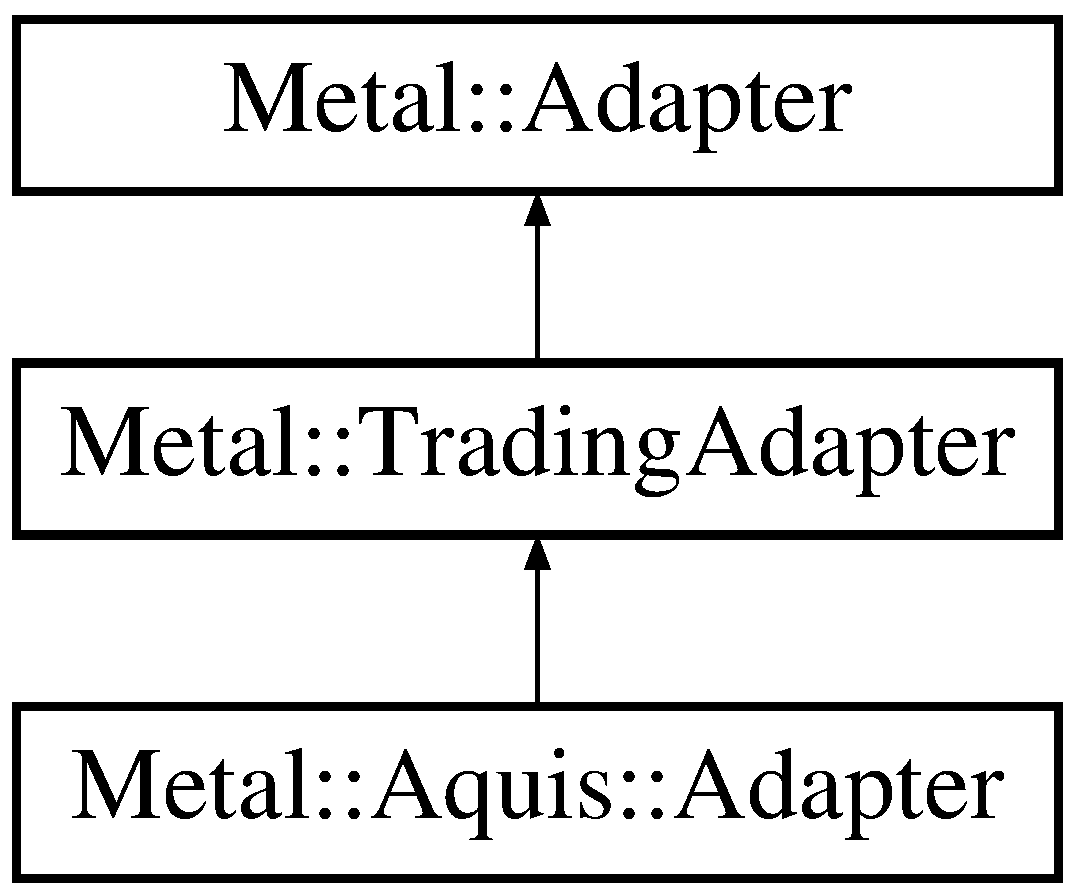
\includegraphics[height=3.000000cm]{classMetal_1_1Aquis_1_1Adapter}
\end{center}
\end{figure}
\subsection*{Public Member Functions}
\begin{DoxyCompactItemize}
\item 
\hyperlink{classMetal_1_1Aquis_1_1Adapter_a20acfdbceb83248f25dc07ffde16b222}{Adapter} ()
\item 
void \hyperlink{classMetal_1_1Aquis_1_1Adapter_a02231f77b67936968df728ea94837224}{encode} (const \hyperlink{classMetal_1_1NewOrderSingle}{New\+Order\+Single} \&nos, \hyperlink{classMetal_1_1Message}{Message} \&msg)
\item 
void \hyperlink{classMetal_1_1Aquis_1_1Adapter_a3cd85e9d1fd5f69b00d9f55b2ce3120b}{encode\+Logon} (\hyperlink{classMetal_1_1Message}{Message} \&msg)
\item 
virtual void \hyperlink{classMetal_1_1Aquis_1_1Adapter_ab7b5bd731548893899e192907f431553}{recv} (const \hyperlink{namespaceMetal_af4294c176f6aecf9f75e9b106b117aa1}{Execution\+Report} \&er)
\item 
virtual \hyperlink{classMetal_1_1Aquis_1_1Adapter_ac5ba9ce761529573d07804f419d56576}{$\sim$\+Adapter} ()
\end{DoxyCompactItemize}
\subsection*{Additional Inherited Members}


\subsection{Constructor \& Destructor Documentation}
\hypertarget{classMetal_1_1Aquis_1_1Adapter_a20acfdbceb83248f25dc07ffde16b222}{}\index{Metal\+::\+Aquis\+::\+Adapter@{Metal\+::\+Aquis\+::\+Adapter}!Adapter@{Adapter}}
\index{Adapter@{Adapter}!Metal\+::\+Aquis\+::\+Adapter@{Metal\+::\+Aquis\+::\+Adapter}}
\subsubsection[{Adapter}]{\setlength{\rightskip}{0pt plus 5cm}Metal\+::\+Aquis\+::\+Adapter\+::\+Adapter (
\begin{DoxyParamCaption}
{}
\end{DoxyParamCaption}
)}\label{classMetal_1_1Aquis_1_1Adapter_a20acfdbceb83248f25dc07ffde16b222}
If you have doubts about U\+U\+I\+D, check out header file \hypertarget{classMetal_1_1Aquis_1_1Adapter_ac5ba9ce761529573d07804f419d56576}{}\index{Metal\+::\+Aquis\+::\+Adapter@{Metal\+::\+Aquis\+::\+Adapter}!````~Adapter@{$\sim$\+Adapter}}
\index{````~Adapter@{$\sim$\+Adapter}!Metal\+::\+Aquis\+::\+Adapter@{Metal\+::\+Aquis\+::\+Adapter}}
\subsubsection[{$\sim$\+Adapter}]{\setlength{\rightskip}{0pt plus 5cm}virtual Metal\+::\+Aquis\+::\+Adapter\+::$\sim$\+Adapter (
\begin{DoxyParamCaption}
{}
\end{DoxyParamCaption}
)\hspace{0.3cm}{\ttfamily [inline]}, {\ttfamily [virtual]}}\label{classMetal_1_1Aquis_1_1Adapter_ac5ba9ce761529573d07804f419d56576}


\subsection{Member Function Documentation}
\hypertarget{classMetal_1_1Aquis_1_1Adapter_a02231f77b67936968df728ea94837224}{}\index{Metal\+::\+Aquis\+::\+Adapter@{Metal\+::\+Aquis\+::\+Adapter}!encode@{encode}}
\index{encode@{encode}!Metal\+::\+Aquis\+::\+Adapter@{Metal\+::\+Aquis\+::\+Adapter}}
\subsubsection[{encode}]{\setlength{\rightskip}{0pt plus 5cm}void Metal\+::\+Aquis\+::\+Adapter\+::encode (
\begin{DoxyParamCaption}
\item[{const {\bf New\+Order\+Single} \&}]{nos, }
\item[{{\bf Message} \&}]{msg}
\end{DoxyParamCaption}
)}\label{classMetal_1_1Aquis_1_1Adapter_a02231f77b67936968df728ea94837224}
\hypertarget{classMetal_1_1Aquis_1_1Adapter_a3cd85e9d1fd5f69b00d9f55b2ce3120b}{}\index{Metal\+::\+Aquis\+::\+Adapter@{Metal\+::\+Aquis\+::\+Adapter}!encode\+Logon@{encode\+Logon}}
\index{encode\+Logon@{encode\+Logon}!Metal\+::\+Aquis\+::\+Adapter@{Metal\+::\+Aquis\+::\+Adapter}}
\subsubsection[{encode\+Logon}]{\setlength{\rightskip}{0pt plus 5cm}void Metal\+::\+Aquis\+::\+Adapter\+::encode\+Logon (
\begin{DoxyParamCaption}
\item[{{\bf Message} \&}]{msg}
\end{DoxyParamCaption}
)}\label{classMetal_1_1Aquis_1_1Adapter_a3cd85e9d1fd5f69b00d9f55b2ce3120b}
\hypertarget{classMetal_1_1Aquis_1_1Adapter_ab7b5bd731548893899e192907f431553}{}\index{Metal\+::\+Aquis\+::\+Adapter@{Metal\+::\+Aquis\+::\+Adapter}!recv@{recv}}
\index{recv@{recv}!Metal\+::\+Aquis\+::\+Adapter@{Metal\+::\+Aquis\+::\+Adapter}}
\subsubsection[{recv}]{\setlength{\rightskip}{0pt plus 5cm}void Metal\+::\+Aquis\+::\+Adapter\+::recv (
\begin{DoxyParamCaption}
\item[{const {\bf Execution\+Report} \&}]{er}
\end{DoxyParamCaption}
)\hspace{0.3cm}{\ttfamily [virtual]}}\label{classMetal_1_1Aquis_1_1Adapter_ab7b5bd731548893899e192907f431553}


The documentation for this class was generated from the following files\+:\begin{DoxyCompactItemize}
\item 
/home/jc/metal/github/src/adapters/\+Aquis\+A\+T\+P\+Adapter/\hyperlink{src_2adapters_2AquisATPAdapter_2Adapter_8h}{Adapter.\+h}\item 
/home/jc/metal/github/src/adapters/\+Aquis\+A\+T\+P\+Adapter/\hyperlink{adapters_2AquisATPAdapter_2Adapter_8cpp}{Adapter.\+cpp}\end{DoxyCompactItemize}

\hypertarget{classMetal_1_1Adapter}{}\section{Metal\+:\+:Adapter Class Reference}
\label{classMetal_1_1Adapter}\index{Metal\+::\+Adapter@{Metal\+::\+Adapter}}
Inheritance diagram for Metal\+:\+:Adapter\+:\begin{figure}[H]
\begin{center}
\leavevmode
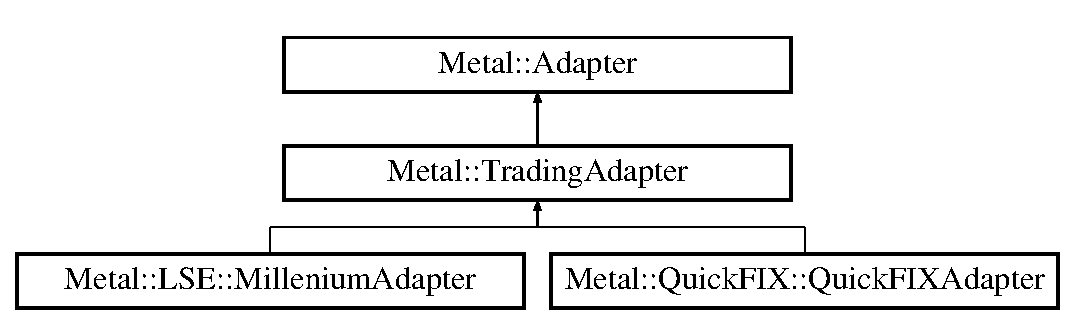
\includegraphics[height=3.000000cm]{classMetal_1_1Adapter}
\end{center}
\end{figure}
\subsection*{Public Member Functions}
\begin{DoxyCompactItemize}
\item 
\hyperlink{classMetal_1_1Adapter_a04519bef3780569a6e1bd26865b69577}{Adapter} (const std\+::string \&name\+Param, const std\+::string \&uuid\+Param)
\item 
\hypertarget{classMetal_1_1Adapter_a548dd70ecda0b21ddf3a459719d10377}{}const std\+::string \& {\bfseries get\+Name} ()\label{classMetal_1_1Adapter_a548dd70ecda0b21ddf3a459719d10377}

\item 
const std\+::string \& \hyperlink{classMetal_1_1Adapter_acd274a92f404cdc435a4d7030a7b1b58}{get\+U\+U\+I\+D} ()
\item 
\hypertarget{classMetal_1_1Adapter_a2c51b1d584d5110384782e4d535f52dc}{}virtual void {\bfseries start} ()=0\label{classMetal_1_1Adapter_a2c51b1d584d5110384782e4d535f52dc}

\item 
\hypertarget{classMetal_1_1Adapter_afac53c6c3aa80b5d09519b1daa0ccf86}{}virtual void {\bfseries stop} ()=0\label{classMetal_1_1Adapter_afac53c6c3aa80b5d09519b1daa0ccf86}

\end{DoxyCompactItemize}
\subsection*{Protected Attributes}
\begin{DoxyCompactItemize}
\item 
\hypertarget{classMetal_1_1Adapter_a6f0924d1c38de9c07c2fee73ce75d5f6}{}std\+::string {\bfseries name}\label{classMetal_1_1Adapter_a6f0924d1c38de9c07c2fee73ce75d5f6}

\item 
\hypertarget{classMetal_1_1Adapter_a20096a0f4ad14b746ca2e1f58ac4a969}{}std\+::string {\bfseries uuid}\label{classMetal_1_1Adapter_a20096a0f4ad14b746ca2e1f58ac4a969}

\end{DoxyCompactItemize}


\subsection{Constructor \& Destructor Documentation}
\hypertarget{classMetal_1_1Adapter_a04519bef3780569a6e1bd26865b69577}{}\index{Metal\+::\+Adapter@{Metal\+::\+Adapter}!Adapter@{Adapter}}
\index{Adapter@{Adapter}!Metal\+::\+Adapter@{Metal\+::\+Adapter}}
\subsubsection[{Adapter}]{\setlength{\rightskip}{0pt plus 5cm}Metal\+::\+Adapter\+::\+Adapter (
\begin{DoxyParamCaption}
\item[{const std\+::string \&}]{name\+Param, }
\item[{const std\+::string \&}]{uuid\+Param}
\end{DoxyParamCaption}
)\hspace{0.3cm}{\ttfamily [inline]}}\label{classMetal_1_1Adapter_a04519bef3780569a6e1bd26865b69577}

\begin{DoxyParams}{Parameters}
{\em } & \\
\hline
\end{DoxyParams}


\subsection{Member Function Documentation}
\hypertarget{classMetal_1_1Adapter_acd274a92f404cdc435a4d7030a7b1b58}{}\index{Metal\+::\+Adapter@{Metal\+::\+Adapter}!get\+U\+U\+I\+D@{get\+U\+U\+I\+D}}
\index{get\+U\+U\+I\+D@{get\+U\+U\+I\+D}!Metal\+::\+Adapter@{Metal\+::\+Adapter}}
\subsubsection[{get\+U\+U\+I\+D}]{\setlength{\rightskip}{0pt plus 5cm}const std\+::string\& Metal\+::\+Adapter\+::get\+U\+U\+I\+D (
\begin{DoxyParamCaption}
{}
\end{DoxyParamCaption}
)\hspace{0.3cm}{\ttfamily [inline]}}\label{classMetal_1_1Adapter_acd274a92f404cdc435a4d7030a7b1b58}
Retrieve Unique I\+D For example, this is used by benchmarking to report results~\newline
 This is also used on the web site to identify adapters. 

The documentation for this class was generated from the following file\+:\begin{DoxyCompactItemize}
\item 
/home/jc/metal/src/metal/Adapter.\+h\end{DoxyCompactItemize}

\hypertarget{classMetal_1_1Aquis_1_1Codec}{}\section{Metal\+:\+:Aquis\+:\+:Codec Class Reference}
\label{classMetal_1_1Aquis_1_1Codec}\index{Metal\+::\+Aquis\+::\+Codec@{Metal\+::\+Aquis\+::\+Codec}}


{\ttfamily \#include $<$Codec.\+h$>$}

Inheritance diagram for Metal\+:\+:Aquis\+:\+:Codec\+:\begin{figure}[H]
\begin{center}
\leavevmode
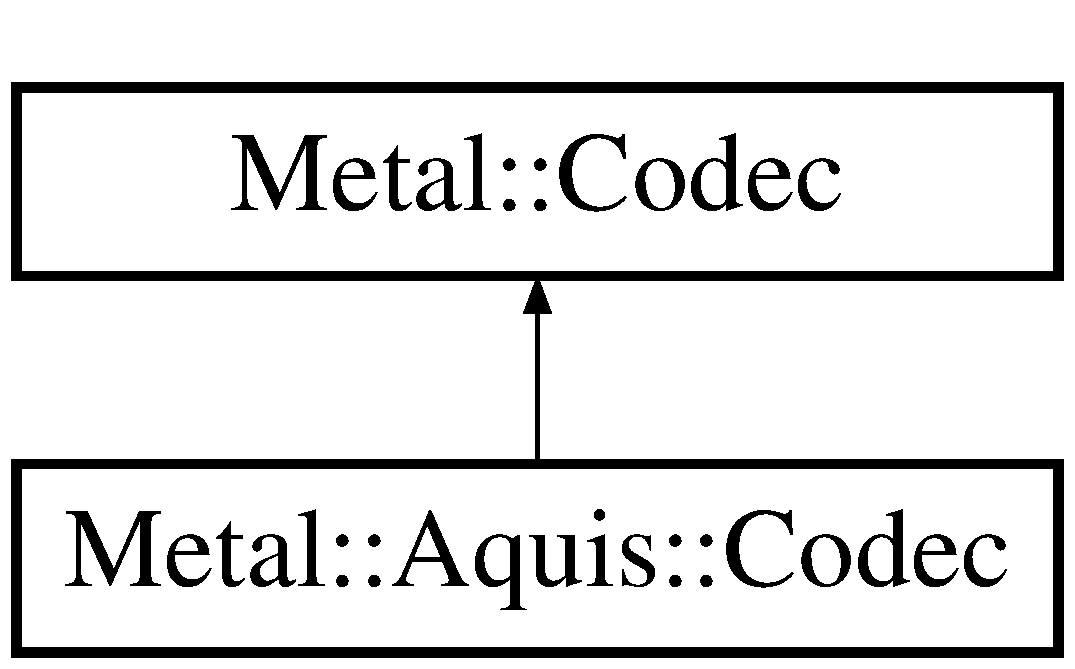
\includegraphics[height=2.000000cm]{classMetal_1_1Aquis_1_1Codec}
\end{center}
\end{figure}
\subsection*{Public Member Functions}
\begin{DoxyCompactItemize}
\item 
\hyperlink{classMetal_1_1Aquis_1_1Codec_ab68190600daa2d1b8105e6d8ff83afd6}{Codec} ()
\item 
virtual \hyperlink{classMetal_1_1Aquis_1_1Codec_a7bdeb61cbb583a2a77476cd7b196c0c2}{$\sim$\+Codec} ()
\item 
void \hyperlink{classMetal_1_1Aquis_1_1Codec_a361dc20ec705f056891468c8b0312699}{encode} (const \hyperlink{classMetal_1_1Aquis_1_1OrderCancel}{Order\+Cancel} \&oc, \hyperlink{namespaceMetal_1_1Aquis_a2e28795915a9bf76ccc4574a24376487}{Seq\+Num} seq\+Num, \hyperlink{classMetal_1_1Message}{Message} \&msg)
\item 
void \hyperlink{classMetal_1_1Aquis_1_1Codec_aaf73f35bd28f5f59ac6b2a968354bb91}{encode} (const \hyperlink{classMetal_1_1Aquis_1_1OrderAdd}{Order\+Add} \&oa, \hyperlink{namespaceMetal_1_1Aquis_a2e28795915a9bf76ccc4574a24376487}{Seq\+Num} seq\+Num, \hyperlink{classMetal_1_1Message}{Message} \&msg)
\item 
void \hyperlink{classMetal_1_1Aquis_1_1Codec_a1162f3fd1a0f6351dba465a23af0f114}{encode} (const \hyperlink{classMetal_1_1Aquis_1_1Login}{Login} \&login, \hyperlink{namespaceMetal_1_1Aquis_a2e28795915a9bf76ccc4574a24376487}{Seq\+Num} seq\+Num, \hyperlink{classMetal_1_1Message}{Message} \&msg)
\item 
void \hyperlink{classMetal_1_1Aquis_1_1Codec_a8aa920b8a5422358a2529056e36094d7}{encode} (const uint16\+\_\+t \&i, \hyperlink{classMetal_1_1Message}{Message} \&msg, int position)
\item 
void \hyperlink{classMetal_1_1Aquis_1_1Codec_a82ef20e51a8850db3213c60a9348b59e}{encode} (const uint32\+\_\+t \&i, \hyperlink{classMetal_1_1Message}{Message} \&msg, int position)
\item 
void \hyperlink{classMetal_1_1Aquis_1_1Codec_abd44b89febe2913fbe8505653ce17cb4}{encode} (const uint64\+\_\+t \&i, \hyperlink{classMetal_1_1Message}{Message} \&msg, int position)
\item 
void \hyperlink{classMetal_1_1Aquis_1_1Codec_ae0e2296c1a295fa7f6000e94d8cc7f13}{encode\+Header} (\hyperlink{namespaceMetal_1_1Aquis_ac6c095b7eefa1d7918de0fe9387f3786}{Msg\+Type} type, uint16\+\_\+t length, \hyperlink{namespaceMetal_1_1Aquis_a2e28795915a9bf76ccc4574a24376487}{Seq\+Num} seq\+Num, \hyperlink{classMetal_1_1Message}{Message} \&msg)
\end{DoxyCompactItemize}
\subsection*{Additional Inherited Members}


\subsection{Constructor \& Destructor Documentation}
\hypertarget{classMetal_1_1Aquis_1_1Codec_ab68190600daa2d1b8105e6d8ff83afd6}{}\index{Metal\+::\+Aquis\+::\+Codec@{Metal\+::\+Aquis\+::\+Codec}!Codec@{Codec}}
\index{Codec@{Codec}!Metal\+::\+Aquis\+::\+Codec@{Metal\+::\+Aquis\+::\+Codec}}
\subsubsection[{Codec}]{\setlength{\rightskip}{0pt plus 5cm}Metal\+::\+Aquis\+::\+Codec\+::\+Codec (
\begin{DoxyParamCaption}
{}
\end{DoxyParamCaption}
)}\label{classMetal_1_1Aquis_1_1Codec_ab68190600daa2d1b8105e6d8ff83afd6}
\hypertarget{classMetal_1_1Aquis_1_1Codec_a7bdeb61cbb583a2a77476cd7b196c0c2}{}\index{Metal\+::\+Aquis\+::\+Codec@{Metal\+::\+Aquis\+::\+Codec}!````~Codec@{$\sim$\+Codec}}
\index{````~Codec@{$\sim$\+Codec}!Metal\+::\+Aquis\+::\+Codec@{Metal\+::\+Aquis\+::\+Codec}}
\subsubsection[{$\sim$\+Codec}]{\setlength{\rightskip}{0pt plus 5cm}Metal\+::\+Aquis\+::\+Codec\+::$\sim$\+Codec (
\begin{DoxyParamCaption}
{}
\end{DoxyParamCaption}
)\hspace{0.3cm}{\ttfamily [virtual]}}\label{classMetal_1_1Aquis_1_1Codec_a7bdeb61cbb583a2a77476cd7b196c0c2}


Reimplemented from \hyperlink{classMetal_1_1Codec_a68847484c9c80e04e4e4e5592cf113db}{Metal\+::\+Codec}.



\subsection{Member Function Documentation}
\hypertarget{classMetal_1_1Aquis_1_1Codec_a361dc20ec705f056891468c8b0312699}{}\index{Metal\+::\+Aquis\+::\+Codec@{Metal\+::\+Aquis\+::\+Codec}!encode@{encode}}
\index{encode@{encode}!Metal\+::\+Aquis\+::\+Codec@{Metal\+::\+Aquis\+::\+Codec}}
\subsubsection[{encode}]{\setlength{\rightskip}{0pt plus 5cm}void Metal\+::\+Aquis\+::\+Codec\+::encode (
\begin{DoxyParamCaption}
\item[{const {\bf Order\+Cancel} \&}]{oc, }
\item[{{\bf Seq\+Num}}]{seq\+Num, }
\item[{{\bf Message} \&}]{msg}
\end{DoxyParamCaption}
)}\label{classMetal_1_1Aquis_1_1Codec_a361dc20ec705f056891468c8b0312699}
Encodes a cancel request 
\begin{DoxyParams}{Parameters}
{\em oc} & The Order Cancel representation \\
\hline
{\em seq\+Num} & the current sequence number \\
\hline
{\em msg} & The destination message \\
\hline
\end{DoxyParams}
\hypertarget{classMetal_1_1Aquis_1_1Codec_aaf73f35bd28f5f59ac6b2a968354bb91}{}\index{Metal\+::\+Aquis\+::\+Codec@{Metal\+::\+Aquis\+::\+Codec}!encode@{encode}}
\index{encode@{encode}!Metal\+::\+Aquis\+::\+Codec@{Metal\+::\+Aquis\+::\+Codec}}
\subsubsection[{encode}]{\setlength{\rightskip}{0pt plus 5cm}void Metal\+::\+Aquis\+::\+Codec\+::encode (
\begin{DoxyParamCaption}
\item[{const {\bf Order\+Add} \&}]{oa, }
\item[{{\bf Seq\+Num}}]{seq\+Num, }
\item[{{\bf Message} \&}]{msg}
\end{DoxyParamCaption}
)}\label{classMetal_1_1Aquis_1_1Codec_aaf73f35bd28f5f59ac6b2a968354bb91}
Encodes a new order 
\begin{DoxyParams}{Parameters}
{\em oq} & The Order Add representation \\
\hline
{\em seq\+Num} & the current sequence number \\
\hline
{\em msg} & The destination message \\
\hline
\end{DoxyParams}
\hypertarget{classMetal_1_1Aquis_1_1Codec_a1162f3fd1a0f6351dba465a23af0f114}{}\index{Metal\+::\+Aquis\+::\+Codec@{Metal\+::\+Aquis\+::\+Codec}!encode@{encode}}
\index{encode@{encode}!Metal\+::\+Aquis\+::\+Codec@{Metal\+::\+Aquis\+::\+Codec}}
\subsubsection[{encode}]{\setlength{\rightskip}{0pt plus 5cm}void Metal\+::\+Aquis\+::\+Codec\+::encode (
\begin{DoxyParamCaption}
\item[{const {\bf Login} \&}]{login, }
\item[{{\bf Seq\+Num}}]{seq\+Num, }
\item[{{\bf Message} \&}]{msg}
\end{DoxyParamCaption}
)}\label{classMetal_1_1Aquis_1_1Codec_a1162f3fd1a0f6351dba465a23af0f114}
Encodes a login 
\begin{DoxyParams}{Parameters}
{\em login} & \hyperlink{classMetal_1_1Aquis_1_1Login}{Login} representation. Must be constructed with all values \\
\hline
{\em seq\+Num} & The sequence number \\
\hline
{\em msg} & The destination message \\
\hline
\end{DoxyParams}
\hypertarget{classMetal_1_1Aquis_1_1Codec_a8aa920b8a5422358a2529056e36094d7}{}\index{Metal\+::\+Aquis\+::\+Codec@{Metal\+::\+Aquis\+::\+Codec}!encode@{encode}}
\index{encode@{encode}!Metal\+::\+Aquis\+::\+Codec@{Metal\+::\+Aquis\+::\+Codec}}
\subsubsection[{encode}]{\setlength{\rightskip}{0pt plus 5cm}void Metal\+::\+Aquis\+::\+Codec\+::encode (
\begin{DoxyParamCaption}
\item[{const uint16\+\_\+t \&}]{i, }
\item[{{\bf Message} \&}]{msg, }
\item[{int}]{position}
\end{DoxyParamCaption}
)\hspace{0.3cm}{\ttfamily [inline]}}\label{classMetal_1_1Aquis_1_1Codec_a8aa920b8a5422358a2529056e36094d7}
\hypertarget{classMetal_1_1Aquis_1_1Codec_a82ef20e51a8850db3213c60a9348b59e}{}\index{Metal\+::\+Aquis\+::\+Codec@{Metal\+::\+Aquis\+::\+Codec}!encode@{encode}}
\index{encode@{encode}!Metal\+::\+Aquis\+::\+Codec@{Metal\+::\+Aquis\+::\+Codec}}
\subsubsection[{encode}]{\setlength{\rightskip}{0pt plus 5cm}void Metal\+::\+Aquis\+::\+Codec\+::encode (
\begin{DoxyParamCaption}
\item[{const uint32\+\_\+t \&}]{i, }
\item[{{\bf Message} \&}]{msg, }
\item[{int}]{position}
\end{DoxyParamCaption}
)\hspace{0.3cm}{\ttfamily [inline]}}\label{classMetal_1_1Aquis_1_1Codec_a82ef20e51a8850db3213c60a9348b59e}
\hypertarget{classMetal_1_1Aquis_1_1Codec_abd44b89febe2913fbe8505653ce17cb4}{}\index{Metal\+::\+Aquis\+::\+Codec@{Metal\+::\+Aquis\+::\+Codec}!encode@{encode}}
\index{encode@{encode}!Metal\+::\+Aquis\+::\+Codec@{Metal\+::\+Aquis\+::\+Codec}}
\subsubsection[{encode}]{\setlength{\rightskip}{0pt plus 5cm}void Metal\+::\+Aquis\+::\+Codec\+::encode (
\begin{DoxyParamCaption}
\item[{const uint64\+\_\+t \&}]{i, }
\item[{{\bf Message} \&}]{msg, }
\item[{int}]{position}
\end{DoxyParamCaption}
)\hspace{0.3cm}{\ttfamily [inline]}}\label{classMetal_1_1Aquis_1_1Codec_abd44b89febe2913fbe8505653ce17cb4}
\hypertarget{classMetal_1_1Aquis_1_1Codec_ae0e2296c1a295fa7f6000e94d8cc7f13}{}\index{Metal\+::\+Aquis\+::\+Codec@{Metal\+::\+Aquis\+::\+Codec}!encode\+Header@{encode\+Header}}
\index{encode\+Header@{encode\+Header}!Metal\+::\+Aquis\+::\+Codec@{Metal\+::\+Aquis\+::\+Codec}}
\subsubsection[{encode\+Header}]{\setlength{\rightskip}{0pt plus 5cm}void Metal\+::\+Aquis\+::\+Codec\+::encode\+Header (
\begin{DoxyParamCaption}
\item[{{\bf Msg\+Type}}]{type, }
\item[{uint16\+\_\+t}]{length, }
\item[{{\bf Seq\+Num}}]{seq\+Num, }
\item[{{\bf Message} \&}]{msg}
\end{DoxyParamCaption}
)\hspace{0.3cm}{\ttfamily [inline]}}\label{classMetal_1_1Aquis_1_1Codec_ae0e2296c1a295fa7f6000e94d8cc7f13}
Encode \hyperlink{namespaceMetal_1_1Aquis}{Aquis} A\+T\+P Header 
\begin{DoxyParams}{Parameters}
{\em length} & full message length \\
\hline
{\em seq\+Num} & \hyperlink{classMetal_1_1Message}{Message} sequence number \\
\hline
{\em type} & \hyperlink{classMetal_1_1Message}{Message} Type \\
\hline
{\em msg} & the output message \\
\hline
\end{DoxyParams}


The documentation for this class was generated from the following files\+:\begin{DoxyCompactItemize}
\item 
/home/jc/metal/github/src/adapters/\+Aquis\+A\+T\+P\+Adapter/\hyperlink{src_2adapters_2AquisATPAdapter_2Codec_8h}{Codec.\+h}\item 
/home/jc/metal/github/src/adapters/\+Aquis\+A\+T\+P\+Adapter/\hyperlink{adapters_2AquisATPAdapter_2Codec_8cpp}{Codec.\+cpp}\end{DoxyCompactItemize}

\hypertarget{classMetal_1_1Codec}{}\section{Metal\+:\+:Codec Class Reference}
\label{classMetal_1_1Codec}\index{Metal\+::\+Codec@{Metal\+::\+Codec}}


{\ttfamily \#include $<$Codec.\+h$>$}

Inheritance diagram for Metal\+:\+:Codec\+:\begin{figure}[H]
\begin{center}
\leavevmode
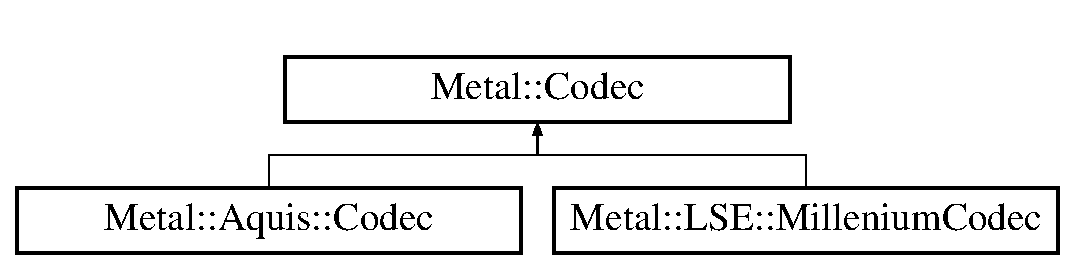
\includegraphics[height=2.000000cm]{classMetal_1_1Codec}
\end{center}
\end{figure}
\subsection*{Public Member Functions}
\begin{DoxyCompactItemize}
\item 
\hyperlink{classMetal_1_1Codec_a439fd8e827fabe656f49a7a043ab98d0}{Codec} ()
\item 
virtual int \hyperlink{classMetal_1_1Codec_a4d532631bde9029d9b5875fccaa5934e}{get\+Message\+Length} (char $\ast$data, int size)
\item 
void \hyperlink{classMetal_1_1Codec_a5b9970f32f2ff95981794993e2293011}{decode} (const char $\ast$data, int position, int8\+\_\+t \&output)
\item 
void \hyperlink{classMetal_1_1Codec_abf3b5c0af60d724c810b72b7dec909ee}{decode} (const char $\ast$data, int position, uint8\+\_\+t \&output)
\item 
void \hyperlink{classMetal_1_1Codec_a3f6d5f3018ae686f80512ad88e9a3329}{decode\+B\+E} (const char $\ast$data, int position, int16\+\_\+t \&output)
\item 
void \hyperlink{classMetal_1_1Codec_a2d51b5e2c7ab2d27ab12de4ac62e9eca}{decode\+B\+E} (const char $\ast$data, int position, uint16\+\_\+t \&output)
\item 
void \hyperlink{classMetal_1_1Codec_aa858a2edfd1227118d696f906746e7a1}{decode\+B\+E} (const char $\ast$data, int position, int32\+\_\+t \&output)
\item 
void \hyperlink{classMetal_1_1Codec_a84257d127b1918965b47e7df825fcfcb}{decode\+B\+E} (const char $\ast$data, int position, uint32\+\_\+t \&output)
\item 
void \hyperlink{classMetal_1_1Codec_a992488cf4e72ff2e26644ee0b719d7a3}{decode\+B\+E} (const char $\ast$data, int position, int64\+\_\+t \&output)
\item 
void \hyperlink{classMetal_1_1Codec_a4af4488934bd2dd20dcc82fbef75cca5}{decode\+B\+E} (const char $\ast$data, int position, uint64\+\_\+t \&output)
\item 
void \hyperlink{classMetal_1_1Codec_a9de32d0f9bbd0c25d3970b1fd748eb08}{decode\+L\+E} (const char $\ast$data, int position, int16\+\_\+t \&output)
\item 
void \hyperlink{classMetal_1_1Codec_afc62b66910d365f4cddcdc2d869371ea}{decode\+L\+E} (const char $\ast$data, int position, uint16\+\_\+t \&output)
\item 
void \hyperlink{classMetal_1_1Codec_ac8f4b899ca5f19400e7acbbf8ba28f33}{decode\+L\+E} (const char $\ast$data, int position, int32\+\_\+t \&output)
\item 
void \hyperlink{classMetal_1_1Codec_aa698a26f90f1f2874183c7b7c90c7b61}{decode\+L\+E} (const char $\ast$data, int position, uint32\+\_\+t \&output)
\item 
void \hyperlink{classMetal_1_1Codec_a1836678a806c987d7d96587a5130b3c6}{decode\+L\+E} (const char $\ast$data, int position, int64\+\_\+t \&output)
\item 
void \hyperlink{classMetal_1_1Codec_ae69549741e857cce3b915c9ef6ab6a7b}{decode\+L\+E} (const char $\ast$data, int position, uint64\+\_\+t \&output)
\item 
void \hyperlink{classMetal_1_1Codec_a22284aa82f334f7e81755dc044e05c58}{decode} (const char $\ast$data, int position, std\+::string \&output, int max\+Length)
\item 
void \hyperlink{classMetal_1_1Codec_aa6be9650e0fc53f01f1c94a771300665}{encode} (const std\+::string \&str, \hyperlink{classMetal_1_1Message}{Message} \&msg, int position, int max\+Length)
\item 
void \hyperlink{classMetal_1_1Codec_a2483a02d8022a4aae4345758244a154b}{encode} (const int8\+\_\+t \&i, \hyperlink{classMetal_1_1Message}{Message} \&msg, int position)
\item 
void \hyperlink{classMetal_1_1Codec_a638c8eccf2d989ea31a0670764b9cb0b}{encode\+L\+E} (const int16\+\_\+t \&i, \hyperlink{classMetal_1_1Message}{Message} \&msg, int position)
\item 
void \hyperlink{classMetal_1_1Codec_a08aafff1f98ec3d4b3c0490606d109f6}{encode\+L\+E} (const uint16\+\_\+t \&i, \hyperlink{classMetal_1_1Message}{Message} \&msg, int position)
\item 
void \hyperlink{classMetal_1_1Codec_a0c3cf0c6a614610c1d56859ea3fadc48}{encode\+B\+E} (const int16\+\_\+t \&i, \hyperlink{classMetal_1_1Message}{Message} \&msg, int position)
\item 
void \hyperlink{classMetal_1_1Codec_a188c8fdc0fb07affe85c8141a5314017}{encode\+B\+E} (const uint16\+\_\+t \&i, \hyperlink{classMetal_1_1Message}{Message} \&msg, int position)
\item 
void \hyperlink{classMetal_1_1Codec_a312401c93d9fdc7ec9468e87534c2f90}{encode\+L\+E} (const int32\+\_\+t \&i, \hyperlink{classMetal_1_1Message}{Message} \&msg, int position)
\item 
void \hyperlink{classMetal_1_1Codec_a5713bcd5042c5ded9e71a336f0ad42bf}{encode\+L\+E} (const uint32\+\_\+t \&i, \hyperlink{classMetal_1_1Message}{Message} \&msg, int position)
\item 
void \hyperlink{classMetal_1_1Codec_a30d84ca7c8a95a10103555b0364d3c0b}{encode\+B\+E} (const int32\+\_\+t \&i, \hyperlink{classMetal_1_1Message}{Message} \&msg, int position)
\item 
void \hyperlink{classMetal_1_1Codec_aa721fe0d642e0a6f127a2c1fc7410293}{encode\+B\+E} (const uint32\+\_\+t \&i, \hyperlink{classMetal_1_1Message}{Message} \&msg, int position)
\item 
void \hyperlink{classMetal_1_1Codec_a32a01360f4aff4c57a7c54c72e1e8a27}{encode\+L\+E} (const int64\+\_\+t \&i, \hyperlink{classMetal_1_1Message}{Message} \&msg, int position)
\item 
void \hyperlink{classMetal_1_1Codec_acbe0a9a61a63cbfc4373b1e72603a70f}{encode\+L\+E} (const uint64\+\_\+t \&i, \hyperlink{classMetal_1_1Message}{Message} \&msg, int position)
\item 
void \hyperlink{classMetal_1_1Codec_afd8c4138467dd3e593e17fe2cbd41a01}{encode\+B\+E} (const int64\+\_\+t \&i, \hyperlink{classMetal_1_1Message}{Message} \&msg, int position)
\item 
void \hyperlink{classMetal_1_1Codec_ae8e4c0fcd43cb06917f833f66e59b413}{encode\+B\+E} (const uint64\+\_\+t \&i, \hyperlink{classMetal_1_1Message}{Message} \&msg, int position)
\item 
virtual void \hyperlink{classMetal_1_1Codec_ae4796fc3d128fa650e28acdfe4277bd7}{encode\+Heart\+Beat} (\hyperlink{classMetal_1_1Message}{Message} \&msg)
\item 
virtual void \hyperlink{classMetal_1_1Codec_a14c3cc3c624726297171e843da71fa83}{encode\+Logon} (\hyperlink{classMetal_1_1Message}{Message} \&msg)
\item 
virtual \hyperlink{classMetal_1_1Codec_a68847484c9c80e04e4e4e5592cf113db}{$\sim$\+Codec} ()
\end{DoxyCompactItemize}
\subsection*{Static Public Member Functions}
\begin{DoxyCompactItemize}
\item 
static std\+::string \hyperlink{classMetal_1_1Codec_afe39c79b73724a05feea4c06a59b4d53}{format\+Hex} (char $\ast$data, int length)
\end{DoxyCompactItemize}


\subsection{Constructor \& Destructor Documentation}
\hypertarget{classMetal_1_1Codec_a439fd8e827fabe656f49a7a043ab98d0}{}\index{Metal\+::\+Codec@{Metal\+::\+Codec}!Codec@{Codec}}
\index{Codec@{Codec}!Metal\+::\+Codec@{Metal\+::\+Codec}}
\subsubsection[{Codec}]{\setlength{\rightskip}{0pt plus 5cm}Metal\+::\+Codec\+::\+Codec (
\begin{DoxyParamCaption}
{}
\end{DoxyParamCaption}
)}\label{classMetal_1_1Codec_a439fd8e827fabe656f49a7a043ab98d0}
\hypertarget{classMetal_1_1Codec_a68847484c9c80e04e4e4e5592cf113db}{}\index{Metal\+::\+Codec@{Metal\+::\+Codec}!````~Codec@{$\sim$\+Codec}}
\index{````~Codec@{$\sim$\+Codec}!Metal\+::\+Codec@{Metal\+::\+Codec}}
\subsubsection[{$\sim$\+Codec}]{\setlength{\rightskip}{0pt plus 5cm}Metal\+::\+Codec\+::$\sim$\+Codec (
\begin{DoxyParamCaption}
{}
\end{DoxyParamCaption}
)\hspace{0.3cm}{\ttfamily [virtual]}}\label{classMetal_1_1Codec_a68847484c9c80e04e4e4e5592cf113db}


Reimplemented in \hyperlink{classMetal_1_1Aquis_1_1Codec_a7bdeb61cbb583a2a77476cd7b196c0c2}{Metal\+::\+Aquis\+::\+Codec}.



\subsection{Member Function Documentation}
\hypertarget{classMetal_1_1Codec_a5b9970f32f2ff95981794993e2293011}{}\index{Metal\+::\+Codec@{Metal\+::\+Codec}!decode@{decode}}
\index{decode@{decode}!Metal\+::\+Codec@{Metal\+::\+Codec}}
\subsubsection[{decode}]{\setlength{\rightskip}{0pt plus 5cm}void Metal\+::\+Codec\+::decode (
\begin{DoxyParamCaption}
\item[{const char $\ast$}]{data, }
\item[{int}]{position, }
\item[{int8\+\_\+t \&}]{output}
\end{DoxyParamCaption}
)\hspace{0.3cm}{\ttfamily [inline]}}\label{classMetal_1_1Codec_a5b9970f32f2ff95981794993e2293011}
Decodes a 8 bits integer from a message \hypertarget{classMetal_1_1Codec_abf3b5c0af60d724c810b72b7dec909ee}{}\index{Metal\+::\+Codec@{Metal\+::\+Codec}!decode@{decode}}
\index{decode@{decode}!Metal\+::\+Codec@{Metal\+::\+Codec}}
\subsubsection[{decode}]{\setlength{\rightskip}{0pt plus 5cm}void Metal\+::\+Codec\+::decode (
\begin{DoxyParamCaption}
\item[{const char $\ast$}]{data, }
\item[{int}]{position, }
\item[{uint8\+\_\+t \&}]{output}
\end{DoxyParamCaption}
)\hspace{0.3cm}{\ttfamily [inline]}}\label{classMetal_1_1Codec_abf3b5c0af60d724c810b72b7dec909ee}
Decodes a 8 bits integer from a message \hypertarget{classMetal_1_1Codec_a22284aa82f334f7e81755dc044e05c58}{}\index{Metal\+::\+Codec@{Metal\+::\+Codec}!decode@{decode}}
\index{decode@{decode}!Metal\+::\+Codec@{Metal\+::\+Codec}}
\subsubsection[{decode}]{\setlength{\rightskip}{0pt plus 5cm}void Metal\+::\+Codec\+::decode (
\begin{DoxyParamCaption}
\item[{const char $\ast$}]{data, }
\item[{int}]{position, }
\item[{std\+::string \&}]{output, }
\item[{int}]{max\+Length}
\end{DoxyParamCaption}
)\hspace{0.3cm}{\ttfamily [inline]}}\label{classMetal_1_1Codec_a22284aa82f334f7e81755dc044e05c58}
Copies data into a string \hypertarget{classMetal_1_1Codec_a3f6d5f3018ae686f80512ad88e9a3329}{}\index{Metal\+::\+Codec@{Metal\+::\+Codec}!decode\+B\+E@{decode\+B\+E}}
\index{decode\+B\+E@{decode\+B\+E}!Metal\+::\+Codec@{Metal\+::\+Codec}}
\subsubsection[{decode\+B\+E}]{\setlength{\rightskip}{0pt plus 5cm}void Metal\+::\+Codec\+::decode\+B\+E (
\begin{DoxyParamCaption}
\item[{const char $\ast$}]{data, }
\item[{int}]{position, }
\item[{int16\+\_\+t \&}]{output}
\end{DoxyParamCaption}
)\hspace{0.3cm}{\ttfamily [inline]}}\label{classMetal_1_1Codec_a3f6d5f3018ae686f80512ad88e9a3329}
Decodes a 16 bits integer from a message in big endian format \hypertarget{classMetal_1_1Codec_a2d51b5e2c7ab2d27ab12de4ac62e9eca}{}\index{Metal\+::\+Codec@{Metal\+::\+Codec}!decode\+B\+E@{decode\+B\+E}}
\index{decode\+B\+E@{decode\+B\+E}!Metal\+::\+Codec@{Metal\+::\+Codec}}
\subsubsection[{decode\+B\+E}]{\setlength{\rightskip}{0pt plus 5cm}void Metal\+::\+Codec\+::decode\+B\+E (
\begin{DoxyParamCaption}
\item[{const char $\ast$}]{data, }
\item[{int}]{position, }
\item[{uint16\+\_\+t \&}]{output}
\end{DoxyParamCaption}
)\hspace{0.3cm}{\ttfamily [inline]}}\label{classMetal_1_1Codec_a2d51b5e2c7ab2d27ab12de4ac62e9eca}
Decodes an unsigned 16 bits integer from a message in big endian format \hypertarget{classMetal_1_1Codec_aa858a2edfd1227118d696f906746e7a1}{}\index{Metal\+::\+Codec@{Metal\+::\+Codec}!decode\+B\+E@{decode\+B\+E}}
\index{decode\+B\+E@{decode\+B\+E}!Metal\+::\+Codec@{Metal\+::\+Codec}}
\subsubsection[{decode\+B\+E}]{\setlength{\rightskip}{0pt plus 5cm}void Metal\+::\+Codec\+::decode\+B\+E (
\begin{DoxyParamCaption}
\item[{const char $\ast$}]{data, }
\item[{int}]{position, }
\item[{int32\+\_\+t \&}]{output}
\end{DoxyParamCaption}
)\hspace{0.3cm}{\ttfamily [inline]}}\label{classMetal_1_1Codec_aa858a2edfd1227118d696f906746e7a1}
Decodes a 32 bits integer from a message in big endian format \hypertarget{classMetal_1_1Codec_a84257d127b1918965b47e7df825fcfcb}{}\index{Metal\+::\+Codec@{Metal\+::\+Codec}!decode\+B\+E@{decode\+B\+E}}
\index{decode\+B\+E@{decode\+B\+E}!Metal\+::\+Codec@{Metal\+::\+Codec}}
\subsubsection[{decode\+B\+E}]{\setlength{\rightskip}{0pt plus 5cm}void Metal\+::\+Codec\+::decode\+B\+E (
\begin{DoxyParamCaption}
\item[{const char $\ast$}]{data, }
\item[{int}]{position, }
\item[{uint32\+\_\+t \&}]{output}
\end{DoxyParamCaption}
)\hspace{0.3cm}{\ttfamily [inline]}}\label{classMetal_1_1Codec_a84257d127b1918965b47e7df825fcfcb}
Decodes an unsigned 32 bits integer from a message in big endian format \hypertarget{classMetal_1_1Codec_a992488cf4e72ff2e26644ee0b719d7a3}{}\index{Metal\+::\+Codec@{Metal\+::\+Codec}!decode\+B\+E@{decode\+B\+E}}
\index{decode\+B\+E@{decode\+B\+E}!Metal\+::\+Codec@{Metal\+::\+Codec}}
\subsubsection[{decode\+B\+E}]{\setlength{\rightskip}{0pt plus 5cm}void Metal\+::\+Codec\+::decode\+B\+E (
\begin{DoxyParamCaption}
\item[{const char $\ast$}]{data, }
\item[{int}]{position, }
\item[{int64\+\_\+t \&}]{output}
\end{DoxyParamCaption}
)\hspace{0.3cm}{\ttfamily [inline]}}\label{classMetal_1_1Codec_a992488cf4e72ff2e26644ee0b719d7a3}
Decodes a 64 bits integer from a message in big endian format \hypertarget{classMetal_1_1Codec_a4af4488934bd2dd20dcc82fbef75cca5}{}\index{Metal\+::\+Codec@{Metal\+::\+Codec}!decode\+B\+E@{decode\+B\+E}}
\index{decode\+B\+E@{decode\+B\+E}!Metal\+::\+Codec@{Metal\+::\+Codec}}
\subsubsection[{decode\+B\+E}]{\setlength{\rightskip}{0pt plus 5cm}void Metal\+::\+Codec\+::decode\+B\+E (
\begin{DoxyParamCaption}
\item[{const char $\ast$}]{data, }
\item[{int}]{position, }
\item[{uint64\+\_\+t \&}]{output}
\end{DoxyParamCaption}
)\hspace{0.3cm}{\ttfamily [inline]}}\label{classMetal_1_1Codec_a4af4488934bd2dd20dcc82fbef75cca5}
Decodes a 64 bits integer from a message in big endian format \hypertarget{classMetal_1_1Codec_a9de32d0f9bbd0c25d3970b1fd748eb08}{}\index{Metal\+::\+Codec@{Metal\+::\+Codec}!decode\+L\+E@{decode\+L\+E}}
\index{decode\+L\+E@{decode\+L\+E}!Metal\+::\+Codec@{Metal\+::\+Codec}}
\subsubsection[{decode\+L\+E}]{\setlength{\rightskip}{0pt plus 5cm}void Metal\+::\+Codec\+::decode\+L\+E (
\begin{DoxyParamCaption}
\item[{const char $\ast$}]{data, }
\item[{int}]{position, }
\item[{int16\+\_\+t \&}]{output}
\end{DoxyParamCaption}
)\hspace{0.3cm}{\ttfamily [inline]}}\label{classMetal_1_1Codec_a9de32d0f9bbd0c25d3970b1fd748eb08}
Decodes a 16 bits integer from a message in little endian format \hypertarget{classMetal_1_1Codec_afc62b66910d365f4cddcdc2d869371ea}{}\index{Metal\+::\+Codec@{Metal\+::\+Codec}!decode\+L\+E@{decode\+L\+E}}
\index{decode\+L\+E@{decode\+L\+E}!Metal\+::\+Codec@{Metal\+::\+Codec}}
\subsubsection[{decode\+L\+E}]{\setlength{\rightskip}{0pt plus 5cm}void Metal\+::\+Codec\+::decode\+L\+E (
\begin{DoxyParamCaption}
\item[{const char $\ast$}]{data, }
\item[{int}]{position, }
\item[{uint16\+\_\+t \&}]{output}
\end{DoxyParamCaption}
)\hspace{0.3cm}{\ttfamily [inline]}}\label{classMetal_1_1Codec_afc62b66910d365f4cddcdc2d869371ea}
Decodes a 16 bits integer from a message in little endian format \hypertarget{classMetal_1_1Codec_ac8f4b899ca5f19400e7acbbf8ba28f33}{}\index{Metal\+::\+Codec@{Metal\+::\+Codec}!decode\+L\+E@{decode\+L\+E}}
\index{decode\+L\+E@{decode\+L\+E}!Metal\+::\+Codec@{Metal\+::\+Codec}}
\subsubsection[{decode\+L\+E}]{\setlength{\rightskip}{0pt plus 5cm}void Metal\+::\+Codec\+::decode\+L\+E (
\begin{DoxyParamCaption}
\item[{const char $\ast$}]{data, }
\item[{int}]{position, }
\item[{int32\+\_\+t \&}]{output}
\end{DoxyParamCaption}
)\hspace{0.3cm}{\ttfamily [inline]}}\label{classMetal_1_1Codec_ac8f4b899ca5f19400e7acbbf8ba28f33}
Decodes a 32 bits integer from a message in little endian format \hypertarget{classMetal_1_1Codec_aa698a26f90f1f2874183c7b7c90c7b61}{}\index{Metal\+::\+Codec@{Metal\+::\+Codec}!decode\+L\+E@{decode\+L\+E}}
\index{decode\+L\+E@{decode\+L\+E}!Metal\+::\+Codec@{Metal\+::\+Codec}}
\subsubsection[{decode\+L\+E}]{\setlength{\rightskip}{0pt plus 5cm}void Metal\+::\+Codec\+::decode\+L\+E (
\begin{DoxyParamCaption}
\item[{const char $\ast$}]{data, }
\item[{int}]{position, }
\item[{uint32\+\_\+t \&}]{output}
\end{DoxyParamCaption}
)\hspace{0.3cm}{\ttfamily [inline]}}\label{classMetal_1_1Codec_aa698a26f90f1f2874183c7b7c90c7b61}
Decodes an unsigned 32 bits integer from a message in little endian format \hypertarget{classMetal_1_1Codec_a1836678a806c987d7d96587a5130b3c6}{}\index{Metal\+::\+Codec@{Metal\+::\+Codec}!decode\+L\+E@{decode\+L\+E}}
\index{decode\+L\+E@{decode\+L\+E}!Metal\+::\+Codec@{Metal\+::\+Codec}}
\subsubsection[{decode\+L\+E}]{\setlength{\rightskip}{0pt plus 5cm}void Metal\+::\+Codec\+::decode\+L\+E (
\begin{DoxyParamCaption}
\item[{const char $\ast$}]{data, }
\item[{int}]{position, }
\item[{int64\+\_\+t \&}]{output}
\end{DoxyParamCaption}
)\hspace{0.3cm}{\ttfamily [inline]}}\label{classMetal_1_1Codec_a1836678a806c987d7d96587a5130b3c6}
Decodes a 64 bits integer from a message in little endian format \hypertarget{classMetal_1_1Codec_ae69549741e857cce3b915c9ef6ab6a7b}{}\index{Metal\+::\+Codec@{Metal\+::\+Codec}!decode\+L\+E@{decode\+L\+E}}
\index{decode\+L\+E@{decode\+L\+E}!Metal\+::\+Codec@{Metal\+::\+Codec}}
\subsubsection[{decode\+L\+E}]{\setlength{\rightskip}{0pt plus 5cm}void Metal\+::\+Codec\+::decode\+L\+E (
\begin{DoxyParamCaption}
\item[{const char $\ast$}]{data, }
\item[{int}]{position, }
\item[{uint64\+\_\+t \&}]{output}
\end{DoxyParamCaption}
)\hspace{0.3cm}{\ttfamily [inline]}}\label{classMetal_1_1Codec_ae69549741e857cce3b915c9ef6ab6a7b}
Decodes an unsigned 64 bits integer from a message in little endian format \hypertarget{classMetal_1_1Codec_aa6be9650e0fc53f01f1c94a771300665}{}\index{Metal\+::\+Codec@{Metal\+::\+Codec}!encode@{encode}}
\index{encode@{encode}!Metal\+::\+Codec@{Metal\+::\+Codec}}
\subsubsection[{encode}]{\setlength{\rightskip}{0pt plus 5cm}void Metal\+::\+Codec\+::encode (
\begin{DoxyParamCaption}
\item[{const std\+::string \&}]{str, }
\item[{{\bf Message} \&}]{msg, }
\item[{int}]{position, }
\item[{int}]{max\+Length}
\end{DoxyParamCaption}
)\hspace{0.3cm}{\ttfamily [inline]}}\label{classMetal_1_1Codec_aa6be9650e0fc53f01f1c94a771300665}
Encode a string up to the given length. 
\begin{DoxyParams}{Parameters}
{\em str} & String to be encoded \\
\hline
\end{DoxyParams}
\hypertarget{classMetal_1_1Codec_a2483a02d8022a4aae4345758244a154b}{}\index{Metal\+::\+Codec@{Metal\+::\+Codec}!encode@{encode}}
\index{encode@{encode}!Metal\+::\+Codec@{Metal\+::\+Codec}}
\subsubsection[{encode}]{\setlength{\rightskip}{0pt plus 5cm}void Metal\+::\+Codec\+::encode (
\begin{DoxyParamCaption}
\item[{const int8\+\_\+t \&}]{i, }
\item[{{\bf Message} \&}]{msg, }
\item[{int}]{position}
\end{DoxyParamCaption}
)\hspace{0.3cm}{\ttfamily [inline]}}\label{classMetal_1_1Codec_a2483a02d8022a4aae4345758244a154b}
\hypertarget{classMetal_1_1Codec_a0c3cf0c6a614610c1d56859ea3fadc48}{}\index{Metal\+::\+Codec@{Metal\+::\+Codec}!encode\+B\+E@{encode\+B\+E}}
\index{encode\+B\+E@{encode\+B\+E}!Metal\+::\+Codec@{Metal\+::\+Codec}}
\subsubsection[{encode\+B\+E}]{\setlength{\rightskip}{0pt plus 5cm}void Metal\+::\+Codec\+::encode\+B\+E (
\begin{DoxyParamCaption}
\item[{const int16\+\_\+t \&}]{i, }
\item[{{\bf Message} \&}]{msg, }
\item[{int}]{position}
\end{DoxyParamCaption}
)\hspace{0.3cm}{\ttfamily [inline]}}\label{classMetal_1_1Codec_a0c3cf0c6a614610c1d56859ea3fadc48}
\hypertarget{classMetal_1_1Codec_a188c8fdc0fb07affe85c8141a5314017}{}\index{Metal\+::\+Codec@{Metal\+::\+Codec}!encode\+B\+E@{encode\+B\+E}}
\index{encode\+B\+E@{encode\+B\+E}!Metal\+::\+Codec@{Metal\+::\+Codec}}
\subsubsection[{encode\+B\+E}]{\setlength{\rightskip}{0pt plus 5cm}void Metal\+::\+Codec\+::encode\+B\+E (
\begin{DoxyParamCaption}
\item[{const uint16\+\_\+t \&}]{i, }
\item[{{\bf Message} \&}]{msg, }
\item[{int}]{position}
\end{DoxyParamCaption}
)\hspace{0.3cm}{\ttfamily [inline]}}\label{classMetal_1_1Codec_a188c8fdc0fb07affe85c8141a5314017}
\hypertarget{classMetal_1_1Codec_a30d84ca7c8a95a10103555b0364d3c0b}{}\index{Metal\+::\+Codec@{Metal\+::\+Codec}!encode\+B\+E@{encode\+B\+E}}
\index{encode\+B\+E@{encode\+B\+E}!Metal\+::\+Codec@{Metal\+::\+Codec}}
\subsubsection[{encode\+B\+E}]{\setlength{\rightskip}{0pt plus 5cm}void Metal\+::\+Codec\+::encode\+B\+E (
\begin{DoxyParamCaption}
\item[{const int32\+\_\+t \&}]{i, }
\item[{{\bf Message} \&}]{msg, }
\item[{int}]{position}
\end{DoxyParamCaption}
)\hspace{0.3cm}{\ttfamily [inline]}}\label{classMetal_1_1Codec_a30d84ca7c8a95a10103555b0364d3c0b}
\hypertarget{classMetal_1_1Codec_aa721fe0d642e0a6f127a2c1fc7410293}{}\index{Metal\+::\+Codec@{Metal\+::\+Codec}!encode\+B\+E@{encode\+B\+E}}
\index{encode\+B\+E@{encode\+B\+E}!Metal\+::\+Codec@{Metal\+::\+Codec}}
\subsubsection[{encode\+B\+E}]{\setlength{\rightskip}{0pt plus 5cm}void Metal\+::\+Codec\+::encode\+B\+E (
\begin{DoxyParamCaption}
\item[{const uint32\+\_\+t \&}]{i, }
\item[{{\bf Message} \&}]{msg, }
\item[{int}]{position}
\end{DoxyParamCaption}
)\hspace{0.3cm}{\ttfamily [inline]}}\label{classMetal_1_1Codec_aa721fe0d642e0a6f127a2c1fc7410293}
\hypertarget{classMetal_1_1Codec_afd8c4138467dd3e593e17fe2cbd41a01}{}\index{Metal\+::\+Codec@{Metal\+::\+Codec}!encode\+B\+E@{encode\+B\+E}}
\index{encode\+B\+E@{encode\+B\+E}!Metal\+::\+Codec@{Metal\+::\+Codec}}
\subsubsection[{encode\+B\+E}]{\setlength{\rightskip}{0pt plus 5cm}void Metal\+::\+Codec\+::encode\+B\+E (
\begin{DoxyParamCaption}
\item[{const int64\+\_\+t \&}]{i, }
\item[{{\bf Message} \&}]{msg, }
\item[{int}]{position}
\end{DoxyParamCaption}
)\hspace{0.3cm}{\ttfamily [inline]}}\label{classMetal_1_1Codec_afd8c4138467dd3e593e17fe2cbd41a01}
\hypertarget{classMetal_1_1Codec_ae8e4c0fcd43cb06917f833f66e59b413}{}\index{Metal\+::\+Codec@{Metal\+::\+Codec}!encode\+B\+E@{encode\+B\+E}}
\index{encode\+B\+E@{encode\+B\+E}!Metal\+::\+Codec@{Metal\+::\+Codec}}
\subsubsection[{encode\+B\+E}]{\setlength{\rightskip}{0pt plus 5cm}void Metal\+::\+Codec\+::encode\+B\+E (
\begin{DoxyParamCaption}
\item[{const uint64\+\_\+t \&}]{i, }
\item[{{\bf Message} \&}]{msg, }
\item[{int}]{position}
\end{DoxyParamCaption}
)\hspace{0.3cm}{\ttfamily [inline]}}\label{classMetal_1_1Codec_ae8e4c0fcd43cb06917f833f66e59b413}
\hypertarget{classMetal_1_1Codec_ae4796fc3d128fa650e28acdfe4277bd7}{}\index{Metal\+::\+Codec@{Metal\+::\+Codec}!encode\+Heart\+Beat@{encode\+Heart\+Beat}}
\index{encode\+Heart\+Beat@{encode\+Heart\+Beat}!Metal\+::\+Codec@{Metal\+::\+Codec}}
\subsubsection[{encode\+Heart\+Beat}]{\setlength{\rightskip}{0pt plus 5cm}virtual void Metal\+::\+Codec\+::encode\+Heart\+Beat (
\begin{DoxyParamCaption}
\item[{{\bf Message} \&}]{msg}
\end{DoxyParamCaption}
)\hspace{0.3cm}{\ttfamily [inline]}, {\ttfamily [virtual]}}\label{classMetal_1_1Codec_ae4796fc3d128fa650e28acdfe4277bd7}
This method should be overriden for exchanges that require a heartbeat~\newline
 
\begin{DoxyParams}{Parameters}
{\em msg} & Where encoded Heart\+Beat \hyperlink{classMetal_1_1Message}{Message} will be stored \\
\hline
\end{DoxyParams}


Reimplemented in \hyperlink{classMetal_1_1LSE_1_1MilleniumCodec_a208c3b0765080cd8fe55b82f9df5a39f}{Metal\+::\+L\+S\+E\+::\+Millenium\+Codec}.

\hypertarget{classMetal_1_1Codec_a638c8eccf2d989ea31a0670764b9cb0b}{}\index{Metal\+::\+Codec@{Metal\+::\+Codec}!encode\+L\+E@{encode\+L\+E}}
\index{encode\+L\+E@{encode\+L\+E}!Metal\+::\+Codec@{Metal\+::\+Codec}}
\subsubsection[{encode\+L\+E}]{\setlength{\rightskip}{0pt plus 5cm}void Metal\+::\+Codec\+::encode\+L\+E (
\begin{DoxyParamCaption}
\item[{const int16\+\_\+t \&}]{i, }
\item[{{\bf Message} \&}]{msg, }
\item[{int}]{position}
\end{DoxyParamCaption}
)\hspace{0.3cm}{\ttfamily [inline]}}\label{classMetal_1_1Codec_a638c8eccf2d989ea31a0670764b9cb0b}
\hypertarget{classMetal_1_1Codec_a08aafff1f98ec3d4b3c0490606d109f6}{}\index{Metal\+::\+Codec@{Metal\+::\+Codec}!encode\+L\+E@{encode\+L\+E}}
\index{encode\+L\+E@{encode\+L\+E}!Metal\+::\+Codec@{Metal\+::\+Codec}}
\subsubsection[{encode\+L\+E}]{\setlength{\rightskip}{0pt plus 5cm}void Metal\+::\+Codec\+::encode\+L\+E (
\begin{DoxyParamCaption}
\item[{const uint16\+\_\+t \&}]{i, }
\item[{{\bf Message} \&}]{msg, }
\item[{int}]{position}
\end{DoxyParamCaption}
)\hspace{0.3cm}{\ttfamily [inline]}}\label{classMetal_1_1Codec_a08aafff1f98ec3d4b3c0490606d109f6}
\hypertarget{classMetal_1_1Codec_a312401c93d9fdc7ec9468e87534c2f90}{}\index{Metal\+::\+Codec@{Metal\+::\+Codec}!encode\+L\+E@{encode\+L\+E}}
\index{encode\+L\+E@{encode\+L\+E}!Metal\+::\+Codec@{Metal\+::\+Codec}}
\subsubsection[{encode\+L\+E}]{\setlength{\rightskip}{0pt plus 5cm}void Metal\+::\+Codec\+::encode\+L\+E (
\begin{DoxyParamCaption}
\item[{const int32\+\_\+t \&}]{i, }
\item[{{\bf Message} \&}]{msg, }
\item[{int}]{position}
\end{DoxyParamCaption}
)\hspace{0.3cm}{\ttfamily [inline]}}\label{classMetal_1_1Codec_a312401c93d9fdc7ec9468e87534c2f90}
\hypertarget{classMetal_1_1Codec_a5713bcd5042c5ded9e71a336f0ad42bf}{}\index{Metal\+::\+Codec@{Metal\+::\+Codec}!encode\+L\+E@{encode\+L\+E}}
\index{encode\+L\+E@{encode\+L\+E}!Metal\+::\+Codec@{Metal\+::\+Codec}}
\subsubsection[{encode\+L\+E}]{\setlength{\rightskip}{0pt plus 5cm}void Metal\+::\+Codec\+::encode\+L\+E (
\begin{DoxyParamCaption}
\item[{const uint32\+\_\+t \&}]{i, }
\item[{{\bf Message} \&}]{msg, }
\item[{int}]{position}
\end{DoxyParamCaption}
)\hspace{0.3cm}{\ttfamily [inline]}}\label{classMetal_1_1Codec_a5713bcd5042c5ded9e71a336f0ad42bf}
\hypertarget{classMetal_1_1Codec_a32a01360f4aff4c57a7c54c72e1e8a27}{}\index{Metal\+::\+Codec@{Metal\+::\+Codec}!encode\+L\+E@{encode\+L\+E}}
\index{encode\+L\+E@{encode\+L\+E}!Metal\+::\+Codec@{Metal\+::\+Codec}}
\subsubsection[{encode\+L\+E}]{\setlength{\rightskip}{0pt plus 5cm}void Metal\+::\+Codec\+::encode\+L\+E (
\begin{DoxyParamCaption}
\item[{const int64\+\_\+t \&}]{i, }
\item[{{\bf Message} \&}]{msg, }
\item[{int}]{position}
\end{DoxyParamCaption}
)\hspace{0.3cm}{\ttfamily [inline]}}\label{classMetal_1_1Codec_a32a01360f4aff4c57a7c54c72e1e8a27}
\hypertarget{classMetal_1_1Codec_acbe0a9a61a63cbfc4373b1e72603a70f}{}\index{Metal\+::\+Codec@{Metal\+::\+Codec}!encode\+L\+E@{encode\+L\+E}}
\index{encode\+L\+E@{encode\+L\+E}!Metal\+::\+Codec@{Metal\+::\+Codec}}
\subsubsection[{encode\+L\+E}]{\setlength{\rightskip}{0pt plus 5cm}void Metal\+::\+Codec\+::encode\+L\+E (
\begin{DoxyParamCaption}
\item[{const uint64\+\_\+t \&}]{i, }
\item[{{\bf Message} \&}]{msg, }
\item[{int}]{position}
\end{DoxyParamCaption}
)\hspace{0.3cm}{\ttfamily [inline]}}\label{classMetal_1_1Codec_acbe0a9a61a63cbfc4373b1e72603a70f}
\hypertarget{classMetal_1_1Codec_a14c3cc3c624726297171e843da71fa83}{}\index{Metal\+::\+Codec@{Metal\+::\+Codec}!encode\+Logon@{encode\+Logon}}
\index{encode\+Logon@{encode\+Logon}!Metal\+::\+Codec@{Metal\+::\+Codec}}
\subsubsection[{encode\+Logon}]{\setlength{\rightskip}{0pt plus 5cm}virtual void Metal\+::\+Codec\+::encode\+Logon (
\begin{DoxyParamCaption}
\item[{{\bf Message} \&}]{msg}
\end{DoxyParamCaption}
)\hspace{0.3cm}{\ttfamily [inline]}, {\ttfamily [virtual]}}\label{classMetal_1_1Codec_a14c3cc3c624726297171e843da71fa83}
This method should be overriden by exchanges that require a logon~\newline
 
\begin{DoxyParams}{Parameters}
{\em msg} & Where encoded \hyperlink{classMetal_1_1Logon}{Logon} \hyperlink{classMetal_1_1Message}{Message} will be stored \\
\hline
\end{DoxyParams}
\hypertarget{classMetal_1_1Codec_afe39c79b73724a05feea4c06a59b4d53}{}\index{Metal\+::\+Codec@{Metal\+::\+Codec}!format\+Hex@{format\+Hex}}
\index{format\+Hex@{format\+Hex}!Metal\+::\+Codec@{Metal\+::\+Codec}}
\subsubsection[{format\+Hex}]{\setlength{\rightskip}{0pt plus 5cm}std\+::string Metal\+::\+Codec\+::format\+Hex (
\begin{DoxyParamCaption}
\item[{char $\ast$}]{data, }
\item[{int}]{length}
\end{DoxyParamCaption}
)\hspace{0.3cm}{\ttfamily [static]}}\label{classMetal_1_1Codec_afe39c79b73724a05feea4c06a59b4d53}
\hypertarget{classMetal_1_1Codec_a4d532631bde9029d9b5875fccaa5934e}{}\index{Metal\+::\+Codec@{Metal\+::\+Codec}!get\+Message\+Length@{get\+Message\+Length}}
\index{get\+Message\+Length@{get\+Message\+Length}!Metal\+::\+Codec@{Metal\+::\+Codec}}
\subsubsection[{get\+Message\+Length}]{\setlength{\rightskip}{0pt plus 5cm}virtual int Metal\+::\+Codec\+::get\+Message\+Length (
\begin{DoxyParamCaption}
\item[{char $\ast$}]{data, }
\item[{int}]{size}
\end{DoxyParamCaption}
)\hspace{0.3cm}{\ttfamily [inline]}, {\ttfamily [virtual]}}\label{classMetal_1_1Codec_a4d532631bde9029d9b5875fccaa5934e}
Find out message length from its wire representation. Will find out message length and copy data into msg bytes. 
\begin{DoxyParams}{Parameters}
{\em data} & Byte array containing data \\
\hline
{\em size} & Number of bytes in array \\
\hline
\end{DoxyParams}
\begin{DoxyReturn}{Returns}
\hyperlink{classMetal_1_1Message}{Message} length or 0 if no message was found in data 
\end{DoxyReturn}


The documentation for this class was generated from the following files\+:\begin{DoxyCompactItemize}
\item 
/home/jc/metal/github/include/metal/\hyperlink{include_2metal_2Codec_8h}{Codec.\+h}\item 
/home/jc/metal/github/src/metal/\hyperlink{metal_2Codec_8cpp}{Codec.\+cpp}\end{DoxyCompactItemize}

\hypertarget{classMetal_1_1LSE_1_1ExecutionReport}{}\section{Metal\+:\+:L\+S\+E\+:\+:Execution\+Report Class Reference}
\label{classMetal_1_1LSE_1_1ExecutionReport}\index{Metal\+::\+L\+S\+E\+::\+Execution\+Report@{Metal\+::\+L\+S\+E\+::\+Execution\+Report}}


{\ttfamily \#include $<$Execution\+Report.\+h$>$}

\subsection*{Public Member Functions}
\begin{DoxyCompactItemize}
\item 
\hyperlink{classMetal_1_1LSE_1_1ExecutionReport_aa6982514c3408004ba864377259775e0}{Execution\+Report} ()
\item 
virtual \hyperlink{classMetal_1_1LSE_1_1ExecutionReport_aefb6a296e2bdbd963e63e1c56243f36e}{$\sim$\+Execution\+Report} ()
\end{DoxyCompactItemize}
\subsection*{Public Attributes}
\begin{DoxyCompactItemize}
\item 
\hyperlink{namespaceMetal_1_1LSE_a89c70e0ff27a052a68a981159295a760}{App\+I\+D} \hyperlink{classMetal_1_1LSE_1_1ExecutionReport_a32b1ba60b6085c239a25612965bc41e9}{app\+I\+D}
\item 
\hyperlink{namespaceMetal_1_1LSE_ab495640332963bbcc53c0c8b3aa48326}{Sequence\+No} \hyperlink{classMetal_1_1LSE_1_1ExecutionReport_af609f1e57c6608c3d570ff849a39e046}{sequence\+No}
\item 
std\+::string \hyperlink{classMetal_1_1LSE_1_1ExecutionReport_a259bc852173731dae6d1e07c75f6f551}{execution\+I\+D}
\item 
std\+::string \hyperlink{classMetal_1_1LSE_1_1ExecutionReport_a1bec67ef726a425c18713a9a95a630ae}{client\+Order\+I\+D}
\item 
std\+::string \hyperlink{classMetal_1_1LSE_1_1ExecutionReport_a45783f7d1498e21889836f303cbd4309}{order\+I\+D}
\item 
\hyperlink{namespaceMetal_1_1LSE_ad5d18db60c5d9498cab95aa9e19a416a}{Exec\+Type} \hyperlink{classMetal_1_1LSE_1_1ExecutionReport_a2bfeb604cc7a6fc10d29dfdd7737eceb}{exec\+Type}
\item 
std\+::string \hyperlink{classMetal_1_1LSE_1_1ExecutionReport_ac32bc52496ed3380bcd84461fd7df2a1}{execution\+Report\+Ref\+I\+D}
\item 
\hyperlink{namespaceMetal_1_1LSE_aaa5d42acc71915dbdbc74bf7b7db958e}{Order\+Status} \hyperlink{classMetal_1_1LSE_1_1ExecutionReport_a92ea50fa59f974b38d71c8fa1c045291}{order\+Status}
\item 
\hyperlink{namespaceMetal_1_1LSE_a4e9785c206e1217535a3c9e223e6b04d}{Order\+Reject\+Code} \hyperlink{classMetal_1_1LSE_1_1ExecutionReport_afef904b5ec57c7aea395adb5c8d4b3e1}{order\+Reject\+Code}
\item 
\hyperlink{namespaceMetal_1_1LSE_a4a629b5e2aed21d653db0debf8b63af4}{Price} \hyperlink{classMetal_1_1LSE_1_1ExecutionReport_a28ca9d73f34fdca2db418208a057d62a}{executed\+Price}
\item 
\hyperlink{namespaceMetal_1_1LSE_a86342859fb8034a9649f6d789e97d9da}{Quantity} \hyperlink{classMetal_1_1LSE_1_1ExecutionReport_a48a4cff027756a079f25e13720069d20}{executed\+Qty}
\item 
\hyperlink{namespaceMetal_1_1LSE_a86342859fb8034a9649f6d789e97d9da}{Quantity} \hyperlink{classMetal_1_1LSE_1_1ExecutionReport_a1abda72cabb0f1fd6ac10586e4681cb7}{leaves\+Qty}
\item 
\hyperlink{namespaceMetal_1_1LSE_ad218510a226f263117710c146016b65b}{Container} \hyperlink{classMetal_1_1LSE_1_1ExecutionReport_afcbe79b4641ebdacbcc696a0d9f7a15a}{container}
\item 
\hyperlink{namespaceMetal_1_1LSE_a86342859fb8034a9649f6d789e97d9da}{Quantity} \hyperlink{classMetal_1_1LSE_1_1ExecutionReport_aae88e278d6a066fc741244ecf9f3ab9d}{display\+Qty}
\item 
\hyperlink{namespaceMetal_1_1LSE_a5280aa41aaa4433df351e733a23ecd14}{Instrument\+I\+D} \hyperlink{classMetal_1_1LSE_1_1ExecutionReport_a18b6d033fd5a94eb6279e1811d11bce9}{instrument\+I\+D}
\item 
\hyperlink{namespaceMetal_1_1LSE_a16935327b8c86efab5ac513a640e8e85}{Restatement\+Reason} \hyperlink{classMetal_1_1LSE_1_1ExecutionReport_a7bf14d524b6b1907bed17d8237e2d945}{restatement\+Reason}
\item 
\hyperlink{namespaceMetal_1_1LSE_af5236b7a999484d8cd5b579b7d7c133b}{Side} \hyperlink{classMetal_1_1LSE_1_1ExecutionReport_a14730831f5ffe625169c09f00c8ae0db}{side}
\item 
std\+::string \hyperlink{classMetal_1_1LSE_1_1ExecutionReport_a89f5bdb1724a80202c89f90ca38d1429}{counterparty}
\item 
\hyperlink{namespaceMetal_1_1LSE_a2230716d38d6562a96dd1b7a53f04c8a}{Trade\+Liquidity\+Indicator} \hyperlink{classMetal_1_1LSE_1_1ExecutionReport_a91963fe4cac5a89e43b6c3e1e5d241a2}{trade\+Liquidity\+Indicator}
\item 
\hyperlink{namespaceMetal_1_1LSE_a9026616462e8f8b2d1b41935d63b1f77}{Trade\+Match\+I\+D} \hyperlink{classMetal_1_1LSE_1_1ExecutionReport_af1a9f56e131ce7a40e4b9789e35f76a7}{trade\+Match\+I\+D}
\item 
\hyperlink{namespaceMetal_1_1LSE_a4f27043d4f3897c99c960b89b5fe8ddb}{Transact\+Time} \hyperlink{classMetal_1_1LSE_1_1ExecutionReport_af53286cedfca6d09c3f4b3a138468861}{transact\+Time}
\item 
\hyperlink{namespaceMetal_1_1LSE_ae826e079e4b4ee205481709e1436a672}{Type\+Of\+Trade} \hyperlink{classMetal_1_1LSE_1_1ExecutionReport_ac792bd8a4c7af225d31b726b3c8c02af}{type\+Of\+Trade}
\item 
\hyperlink{namespaceMetal_1_1LSE_aff7400475e278748e213fefa47bb9b99}{Capacity} \hyperlink{classMetal_1_1LSE_1_1ExecutionReport_ad39330f05bdb249538c67baafa090b17}{capacity}
\item 
\hyperlink{namespaceMetal_1_1LSE_a43d1d8f30663383025e28ce3ca39a19c}{Price\+Differential} \hyperlink{classMetal_1_1LSE_1_1ExecutionReport_aeab170d67c9cc841d12d2888dc42b2d2}{price\+Differential}
\item 
std\+::string \hyperlink{classMetal_1_1LSE_1_1ExecutionReport_ad70be9d164c7b2a61335749efd20626e}{public\+Order\+I\+D}
\end{DoxyCompactItemize}
\subsection*{Static Public Attributes}
\begin{DoxyCompactItemize}
\item 
static const int \hyperlink{classMetal_1_1LSE_1_1ExecutionReport_a004e413fbbed4fe87b7e7636bc7b61af}{S\+I\+Z\+E} = 151
\end{DoxyCompactItemize}


\subsection{Detailed Description}
The purpose of this class is to represent the content of a native \hyperlink{namespaceMetal_1_1LSE}{L\+S\+E} Execution Report message 

\subsection{Constructor \& Destructor Documentation}
\hypertarget{classMetal_1_1LSE_1_1ExecutionReport_aa6982514c3408004ba864377259775e0}{}\index{Metal\+::\+L\+S\+E\+::\+Execution\+Report@{Metal\+::\+L\+S\+E\+::\+Execution\+Report}!Execution\+Report@{Execution\+Report}}
\index{Execution\+Report@{Execution\+Report}!Metal\+::\+L\+S\+E\+::\+Execution\+Report@{Metal\+::\+L\+S\+E\+::\+Execution\+Report}}
\subsubsection[{Execution\+Report}]{\setlength{\rightskip}{0pt plus 5cm}Metal\+::\+L\+S\+E\+::\+Execution\+Report\+::\+Execution\+Report (
\begin{DoxyParamCaption}
{}
\end{DoxyParamCaption}
)}\label{classMetal_1_1LSE_1_1ExecutionReport_aa6982514c3408004ba864377259775e0}
\hypertarget{classMetal_1_1LSE_1_1ExecutionReport_aefb6a296e2bdbd963e63e1c56243f36e}{}\index{Metal\+::\+L\+S\+E\+::\+Execution\+Report@{Metal\+::\+L\+S\+E\+::\+Execution\+Report}!````~Execution\+Report@{$\sim$\+Execution\+Report}}
\index{````~Execution\+Report@{$\sim$\+Execution\+Report}!Metal\+::\+L\+S\+E\+::\+Execution\+Report@{Metal\+::\+L\+S\+E\+::\+Execution\+Report}}
\subsubsection[{$\sim$\+Execution\+Report}]{\setlength{\rightskip}{0pt plus 5cm}Metal\+::\+L\+S\+E\+::\+Execution\+Report\+::$\sim$\+Execution\+Report (
\begin{DoxyParamCaption}
{}
\end{DoxyParamCaption}
)\hspace{0.3cm}{\ttfamily [virtual]}}\label{classMetal_1_1LSE_1_1ExecutionReport_aefb6a296e2bdbd963e63e1c56243f36e}


\subsection{Member Data Documentation}
\hypertarget{classMetal_1_1LSE_1_1ExecutionReport_a32b1ba60b6085c239a25612965bc41e9}{}\index{Metal\+::\+L\+S\+E\+::\+Execution\+Report@{Metal\+::\+L\+S\+E\+::\+Execution\+Report}!app\+I\+D@{app\+I\+D}}
\index{app\+I\+D@{app\+I\+D}!Metal\+::\+L\+S\+E\+::\+Execution\+Report@{Metal\+::\+L\+S\+E\+::\+Execution\+Report}}
\subsubsection[{app\+I\+D}]{\setlength{\rightskip}{0pt plus 5cm}{\bf App\+I\+D} Metal\+::\+L\+S\+E\+::\+Execution\+Report\+::app\+I\+D}\label{classMetal_1_1LSE_1_1ExecutionReport_a32b1ba60b6085c239a25612965bc41e9}
\hypertarget{classMetal_1_1LSE_1_1ExecutionReport_ad39330f05bdb249538c67baafa090b17}{}\index{Metal\+::\+L\+S\+E\+::\+Execution\+Report@{Metal\+::\+L\+S\+E\+::\+Execution\+Report}!capacity@{capacity}}
\index{capacity@{capacity}!Metal\+::\+L\+S\+E\+::\+Execution\+Report@{Metal\+::\+L\+S\+E\+::\+Execution\+Report}}
\subsubsection[{capacity}]{\setlength{\rightskip}{0pt plus 5cm}{\bf Capacity} Metal\+::\+L\+S\+E\+::\+Execution\+Report\+::capacity}\label{classMetal_1_1LSE_1_1ExecutionReport_ad39330f05bdb249538c67baafa090b17}
\hypertarget{classMetal_1_1LSE_1_1ExecutionReport_a1bec67ef726a425c18713a9a95a630ae}{}\index{Metal\+::\+L\+S\+E\+::\+Execution\+Report@{Metal\+::\+L\+S\+E\+::\+Execution\+Report}!client\+Order\+I\+D@{client\+Order\+I\+D}}
\index{client\+Order\+I\+D@{client\+Order\+I\+D}!Metal\+::\+L\+S\+E\+::\+Execution\+Report@{Metal\+::\+L\+S\+E\+::\+Execution\+Report}}
\subsubsection[{client\+Order\+I\+D}]{\setlength{\rightskip}{0pt plus 5cm}std\+::string Metal\+::\+L\+S\+E\+::\+Execution\+Report\+::client\+Order\+I\+D}\label{classMetal_1_1LSE_1_1ExecutionReport_a1bec67ef726a425c18713a9a95a630ae}
\hypertarget{classMetal_1_1LSE_1_1ExecutionReport_afcbe79b4641ebdacbcc696a0d9f7a15a}{}\index{Metal\+::\+L\+S\+E\+::\+Execution\+Report@{Metal\+::\+L\+S\+E\+::\+Execution\+Report}!container@{container}}
\index{container@{container}!Metal\+::\+L\+S\+E\+::\+Execution\+Report@{Metal\+::\+L\+S\+E\+::\+Execution\+Report}}
\subsubsection[{container}]{\setlength{\rightskip}{0pt plus 5cm}{\bf Container} Metal\+::\+L\+S\+E\+::\+Execution\+Report\+::container}\label{classMetal_1_1LSE_1_1ExecutionReport_afcbe79b4641ebdacbcc696a0d9f7a15a}
\hypertarget{classMetal_1_1LSE_1_1ExecutionReport_a89f5bdb1724a80202c89f90ca38d1429}{}\index{Metal\+::\+L\+S\+E\+::\+Execution\+Report@{Metal\+::\+L\+S\+E\+::\+Execution\+Report}!counterparty@{counterparty}}
\index{counterparty@{counterparty}!Metal\+::\+L\+S\+E\+::\+Execution\+Report@{Metal\+::\+L\+S\+E\+::\+Execution\+Report}}
\subsubsection[{counterparty}]{\setlength{\rightskip}{0pt plus 5cm}std\+::string Metal\+::\+L\+S\+E\+::\+Execution\+Report\+::counterparty}\label{classMetal_1_1LSE_1_1ExecutionReport_a89f5bdb1724a80202c89f90ca38d1429}
\hypertarget{classMetal_1_1LSE_1_1ExecutionReport_aae88e278d6a066fc741244ecf9f3ab9d}{}\index{Metal\+::\+L\+S\+E\+::\+Execution\+Report@{Metal\+::\+L\+S\+E\+::\+Execution\+Report}!display\+Qty@{display\+Qty}}
\index{display\+Qty@{display\+Qty}!Metal\+::\+L\+S\+E\+::\+Execution\+Report@{Metal\+::\+L\+S\+E\+::\+Execution\+Report}}
\subsubsection[{display\+Qty}]{\setlength{\rightskip}{0pt plus 5cm}{\bf Quantity} Metal\+::\+L\+S\+E\+::\+Execution\+Report\+::display\+Qty}\label{classMetal_1_1LSE_1_1ExecutionReport_aae88e278d6a066fc741244ecf9f3ab9d}
\hypertarget{classMetal_1_1LSE_1_1ExecutionReport_a2bfeb604cc7a6fc10d29dfdd7737eceb}{}\index{Metal\+::\+L\+S\+E\+::\+Execution\+Report@{Metal\+::\+L\+S\+E\+::\+Execution\+Report}!exec\+Type@{exec\+Type}}
\index{exec\+Type@{exec\+Type}!Metal\+::\+L\+S\+E\+::\+Execution\+Report@{Metal\+::\+L\+S\+E\+::\+Execution\+Report}}
\subsubsection[{exec\+Type}]{\setlength{\rightskip}{0pt plus 5cm}{\bf Exec\+Type} Metal\+::\+L\+S\+E\+::\+Execution\+Report\+::exec\+Type}\label{classMetal_1_1LSE_1_1ExecutionReport_a2bfeb604cc7a6fc10d29dfdd7737eceb}
\hypertarget{classMetal_1_1LSE_1_1ExecutionReport_a28ca9d73f34fdca2db418208a057d62a}{}\index{Metal\+::\+L\+S\+E\+::\+Execution\+Report@{Metal\+::\+L\+S\+E\+::\+Execution\+Report}!executed\+Price@{executed\+Price}}
\index{executed\+Price@{executed\+Price}!Metal\+::\+L\+S\+E\+::\+Execution\+Report@{Metal\+::\+L\+S\+E\+::\+Execution\+Report}}
\subsubsection[{executed\+Price}]{\setlength{\rightskip}{0pt plus 5cm}{\bf Price} Metal\+::\+L\+S\+E\+::\+Execution\+Report\+::executed\+Price}\label{classMetal_1_1LSE_1_1ExecutionReport_a28ca9d73f34fdca2db418208a057d62a}
\hypertarget{classMetal_1_1LSE_1_1ExecutionReport_a48a4cff027756a079f25e13720069d20}{}\index{Metal\+::\+L\+S\+E\+::\+Execution\+Report@{Metal\+::\+L\+S\+E\+::\+Execution\+Report}!executed\+Qty@{executed\+Qty}}
\index{executed\+Qty@{executed\+Qty}!Metal\+::\+L\+S\+E\+::\+Execution\+Report@{Metal\+::\+L\+S\+E\+::\+Execution\+Report}}
\subsubsection[{executed\+Qty}]{\setlength{\rightskip}{0pt plus 5cm}{\bf Quantity} Metal\+::\+L\+S\+E\+::\+Execution\+Report\+::executed\+Qty}\label{classMetal_1_1LSE_1_1ExecutionReport_a48a4cff027756a079f25e13720069d20}
\hypertarget{classMetal_1_1LSE_1_1ExecutionReport_a259bc852173731dae6d1e07c75f6f551}{}\index{Metal\+::\+L\+S\+E\+::\+Execution\+Report@{Metal\+::\+L\+S\+E\+::\+Execution\+Report}!execution\+I\+D@{execution\+I\+D}}
\index{execution\+I\+D@{execution\+I\+D}!Metal\+::\+L\+S\+E\+::\+Execution\+Report@{Metal\+::\+L\+S\+E\+::\+Execution\+Report}}
\subsubsection[{execution\+I\+D}]{\setlength{\rightskip}{0pt plus 5cm}std\+::string Metal\+::\+L\+S\+E\+::\+Execution\+Report\+::execution\+I\+D}\label{classMetal_1_1LSE_1_1ExecutionReport_a259bc852173731dae6d1e07c75f6f551}
\hypertarget{classMetal_1_1LSE_1_1ExecutionReport_ac32bc52496ed3380bcd84461fd7df2a1}{}\index{Metal\+::\+L\+S\+E\+::\+Execution\+Report@{Metal\+::\+L\+S\+E\+::\+Execution\+Report}!execution\+Report\+Ref\+I\+D@{execution\+Report\+Ref\+I\+D}}
\index{execution\+Report\+Ref\+I\+D@{execution\+Report\+Ref\+I\+D}!Metal\+::\+L\+S\+E\+::\+Execution\+Report@{Metal\+::\+L\+S\+E\+::\+Execution\+Report}}
\subsubsection[{execution\+Report\+Ref\+I\+D}]{\setlength{\rightskip}{0pt plus 5cm}std\+::string Metal\+::\+L\+S\+E\+::\+Execution\+Report\+::execution\+Report\+Ref\+I\+D}\label{classMetal_1_1LSE_1_1ExecutionReport_ac32bc52496ed3380bcd84461fd7df2a1}
\hypertarget{classMetal_1_1LSE_1_1ExecutionReport_a18b6d033fd5a94eb6279e1811d11bce9}{}\index{Metal\+::\+L\+S\+E\+::\+Execution\+Report@{Metal\+::\+L\+S\+E\+::\+Execution\+Report}!instrument\+I\+D@{instrument\+I\+D}}
\index{instrument\+I\+D@{instrument\+I\+D}!Metal\+::\+L\+S\+E\+::\+Execution\+Report@{Metal\+::\+L\+S\+E\+::\+Execution\+Report}}
\subsubsection[{instrument\+I\+D}]{\setlength{\rightskip}{0pt plus 5cm}{\bf Instrument\+I\+D} Metal\+::\+L\+S\+E\+::\+Execution\+Report\+::instrument\+I\+D}\label{classMetal_1_1LSE_1_1ExecutionReport_a18b6d033fd5a94eb6279e1811d11bce9}
\hypertarget{classMetal_1_1LSE_1_1ExecutionReport_a1abda72cabb0f1fd6ac10586e4681cb7}{}\index{Metal\+::\+L\+S\+E\+::\+Execution\+Report@{Metal\+::\+L\+S\+E\+::\+Execution\+Report}!leaves\+Qty@{leaves\+Qty}}
\index{leaves\+Qty@{leaves\+Qty}!Metal\+::\+L\+S\+E\+::\+Execution\+Report@{Metal\+::\+L\+S\+E\+::\+Execution\+Report}}
\subsubsection[{leaves\+Qty}]{\setlength{\rightskip}{0pt plus 5cm}{\bf Quantity} Metal\+::\+L\+S\+E\+::\+Execution\+Report\+::leaves\+Qty}\label{classMetal_1_1LSE_1_1ExecutionReport_a1abda72cabb0f1fd6ac10586e4681cb7}
\hypertarget{classMetal_1_1LSE_1_1ExecutionReport_a45783f7d1498e21889836f303cbd4309}{}\index{Metal\+::\+L\+S\+E\+::\+Execution\+Report@{Metal\+::\+L\+S\+E\+::\+Execution\+Report}!order\+I\+D@{order\+I\+D}}
\index{order\+I\+D@{order\+I\+D}!Metal\+::\+L\+S\+E\+::\+Execution\+Report@{Metal\+::\+L\+S\+E\+::\+Execution\+Report}}
\subsubsection[{order\+I\+D}]{\setlength{\rightskip}{0pt plus 5cm}std\+::string Metal\+::\+L\+S\+E\+::\+Execution\+Report\+::order\+I\+D}\label{classMetal_1_1LSE_1_1ExecutionReport_a45783f7d1498e21889836f303cbd4309}
\hypertarget{classMetal_1_1LSE_1_1ExecutionReport_afef904b5ec57c7aea395adb5c8d4b3e1}{}\index{Metal\+::\+L\+S\+E\+::\+Execution\+Report@{Metal\+::\+L\+S\+E\+::\+Execution\+Report}!order\+Reject\+Code@{order\+Reject\+Code}}
\index{order\+Reject\+Code@{order\+Reject\+Code}!Metal\+::\+L\+S\+E\+::\+Execution\+Report@{Metal\+::\+L\+S\+E\+::\+Execution\+Report}}
\subsubsection[{order\+Reject\+Code}]{\setlength{\rightskip}{0pt plus 5cm}{\bf Order\+Reject\+Code} Metal\+::\+L\+S\+E\+::\+Execution\+Report\+::order\+Reject\+Code}\label{classMetal_1_1LSE_1_1ExecutionReport_afef904b5ec57c7aea395adb5c8d4b3e1}
\hypertarget{classMetal_1_1LSE_1_1ExecutionReport_a92ea50fa59f974b38d71c8fa1c045291}{}\index{Metal\+::\+L\+S\+E\+::\+Execution\+Report@{Metal\+::\+L\+S\+E\+::\+Execution\+Report}!order\+Status@{order\+Status}}
\index{order\+Status@{order\+Status}!Metal\+::\+L\+S\+E\+::\+Execution\+Report@{Metal\+::\+L\+S\+E\+::\+Execution\+Report}}
\subsubsection[{order\+Status}]{\setlength{\rightskip}{0pt plus 5cm}{\bf Order\+Status} Metal\+::\+L\+S\+E\+::\+Execution\+Report\+::order\+Status}\label{classMetal_1_1LSE_1_1ExecutionReport_a92ea50fa59f974b38d71c8fa1c045291}
\hypertarget{classMetal_1_1LSE_1_1ExecutionReport_aeab170d67c9cc841d12d2888dc42b2d2}{}\index{Metal\+::\+L\+S\+E\+::\+Execution\+Report@{Metal\+::\+L\+S\+E\+::\+Execution\+Report}!price\+Differential@{price\+Differential}}
\index{price\+Differential@{price\+Differential}!Metal\+::\+L\+S\+E\+::\+Execution\+Report@{Metal\+::\+L\+S\+E\+::\+Execution\+Report}}
\subsubsection[{price\+Differential}]{\setlength{\rightskip}{0pt plus 5cm}{\bf Price\+Differential} Metal\+::\+L\+S\+E\+::\+Execution\+Report\+::price\+Differential}\label{classMetal_1_1LSE_1_1ExecutionReport_aeab170d67c9cc841d12d2888dc42b2d2}
\hypertarget{classMetal_1_1LSE_1_1ExecutionReport_ad70be9d164c7b2a61335749efd20626e}{}\index{Metal\+::\+L\+S\+E\+::\+Execution\+Report@{Metal\+::\+L\+S\+E\+::\+Execution\+Report}!public\+Order\+I\+D@{public\+Order\+I\+D}}
\index{public\+Order\+I\+D@{public\+Order\+I\+D}!Metal\+::\+L\+S\+E\+::\+Execution\+Report@{Metal\+::\+L\+S\+E\+::\+Execution\+Report}}
\subsubsection[{public\+Order\+I\+D}]{\setlength{\rightskip}{0pt plus 5cm}std\+::string Metal\+::\+L\+S\+E\+::\+Execution\+Report\+::public\+Order\+I\+D}\label{classMetal_1_1LSE_1_1ExecutionReport_ad70be9d164c7b2a61335749efd20626e}
\hypertarget{classMetal_1_1LSE_1_1ExecutionReport_a7bf14d524b6b1907bed17d8237e2d945}{}\index{Metal\+::\+L\+S\+E\+::\+Execution\+Report@{Metal\+::\+L\+S\+E\+::\+Execution\+Report}!restatement\+Reason@{restatement\+Reason}}
\index{restatement\+Reason@{restatement\+Reason}!Metal\+::\+L\+S\+E\+::\+Execution\+Report@{Metal\+::\+L\+S\+E\+::\+Execution\+Report}}
\subsubsection[{restatement\+Reason}]{\setlength{\rightskip}{0pt plus 5cm}{\bf Restatement\+Reason} Metal\+::\+L\+S\+E\+::\+Execution\+Report\+::restatement\+Reason}\label{classMetal_1_1LSE_1_1ExecutionReport_a7bf14d524b6b1907bed17d8237e2d945}
\hypertarget{classMetal_1_1LSE_1_1ExecutionReport_af609f1e57c6608c3d570ff849a39e046}{}\index{Metal\+::\+L\+S\+E\+::\+Execution\+Report@{Metal\+::\+L\+S\+E\+::\+Execution\+Report}!sequence\+No@{sequence\+No}}
\index{sequence\+No@{sequence\+No}!Metal\+::\+L\+S\+E\+::\+Execution\+Report@{Metal\+::\+L\+S\+E\+::\+Execution\+Report}}
\subsubsection[{sequence\+No}]{\setlength{\rightskip}{0pt plus 5cm}{\bf Sequence\+No} Metal\+::\+L\+S\+E\+::\+Execution\+Report\+::sequence\+No}\label{classMetal_1_1LSE_1_1ExecutionReport_af609f1e57c6608c3d570ff849a39e046}
\hypertarget{classMetal_1_1LSE_1_1ExecutionReport_a14730831f5ffe625169c09f00c8ae0db}{}\index{Metal\+::\+L\+S\+E\+::\+Execution\+Report@{Metal\+::\+L\+S\+E\+::\+Execution\+Report}!side@{side}}
\index{side@{side}!Metal\+::\+L\+S\+E\+::\+Execution\+Report@{Metal\+::\+L\+S\+E\+::\+Execution\+Report}}
\subsubsection[{side}]{\setlength{\rightskip}{0pt plus 5cm}{\bf Side} Metal\+::\+L\+S\+E\+::\+Execution\+Report\+::side}\label{classMetal_1_1LSE_1_1ExecutionReport_a14730831f5ffe625169c09f00c8ae0db}
\hypertarget{classMetal_1_1LSE_1_1ExecutionReport_a004e413fbbed4fe87b7e7636bc7b61af}{}\index{Metal\+::\+L\+S\+E\+::\+Execution\+Report@{Metal\+::\+L\+S\+E\+::\+Execution\+Report}!S\+I\+Z\+E@{S\+I\+Z\+E}}
\index{S\+I\+Z\+E@{S\+I\+Z\+E}!Metal\+::\+L\+S\+E\+::\+Execution\+Report@{Metal\+::\+L\+S\+E\+::\+Execution\+Report}}
\subsubsection[{S\+I\+Z\+E}]{\setlength{\rightskip}{0pt plus 5cm}const int Metal\+::\+L\+S\+E\+::\+Execution\+Report\+::\+S\+I\+Z\+E = 151\hspace{0.3cm}{\ttfamily [static]}}\label{classMetal_1_1LSE_1_1ExecutionReport_a004e413fbbed4fe87b7e7636bc7b61af}
\hypertarget{classMetal_1_1LSE_1_1ExecutionReport_a91963fe4cac5a89e43b6c3e1e5d241a2}{}\index{Metal\+::\+L\+S\+E\+::\+Execution\+Report@{Metal\+::\+L\+S\+E\+::\+Execution\+Report}!trade\+Liquidity\+Indicator@{trade\+Liquidity\+Indicator}}
\index{trade\+Liquidity\+Indicator@{trade\+Liquidity\+Indicator}!Metal\+::\+L\+S\+E\+::\+Execution\+Report@{Metal\+::\+L\+S\+E\+::\+Execution\+Report}}
\subsubsection[{trade\+Liquidity\+Indicator}]{\setlength{\rightskip}{0pt plus 5cm}{\bf Trade\+Liquidity\+Indicator} Metal\+::\+L\+S\+E\+::\+Execution\+Report\+::trade\+Liquidity\+Indicator}\label{classMetal_1_1LSE_1_1ExecutionReport_a91963fe4cac5a89e43b6c3e1e5d241a2}
\hypertarget{classMetal_1_1LSE_1_1ExecutionReport_af1a9f56e131ce7a40e4b9789e35f76a7}{}\index{Metal\+::\+L\+S\+E\+::\+Execution\+Report@{Metal\+::\+L\+S\+E\+::\+Execution\+Report}!trade\+Match\+I\+D@{trade\+Match\+I\+D}}
\index{trade\+Match\+I\+D@{trade\+Match\+I\+D}!Metal\+::\+L\+S\+E\+::\+Execution\+Report@{Metal\+::\+L\+S\+E\+::\+Execution\+Report}}
\subsubsection[{trade\+Match\+I\+D}]{\setlength{\rightskip}{0pt plus 5cm}{\bf Trade\+Match\+I\+D} Metal\+::\+L\+S\+E\+::\+Execution\+Report\+::trade\+Match\+I\+D}\label{classMetal_1_1LSE_1_1ExecutionReport_af1a9f56e131ce7a40e4b9789e35f76a7}
\hypertarget{classMetal_1_1LSE_1_1ExecutionReport_af53286cedfca6d09c3f4b3a138468861}{}\index{Metal\+::\+L\+S\+E\+::\+Execution\+Report@{Metal\+::\+L\+S\+E\+::\+Execution\+Report}!transact\+Time@{transact\+Time}}
\index{transact\+Time@{transact\+Time}!Metal\+::\+L\+S\+E\+::\+Execution\+Report@{Metal\+::\+L\+S\+E\+::\+Execution\+Report}}
\subsubsection[{transact\+Time}]{\setlength{\rightskip}{0pt plus 5cm}{\bf Transact\+Time} Metal\+::\+L\+S\+E\+::\+Execution\+Report\+::transact\+Time}\label{classMetal_1_1LSE_1_1ExecutionReport_af53286cedfca6d09c3f4b3a138468861}
\hypertarget{classMetal_1_1LSE_1_1ExecutionReport_ac792bd8a4c7af225d31b726b3c8c02af}{}\index{Metal\+::\+L\+S\+E\+::\+Execution\+Report@{Metal\+::\+L\+S\+E\+::\+Execution\+Report}!type\+Of\+Trade@{type\+Of\+Trade}}
\index{type\+Of\+Trade@{type\+Of\+Trade}!Metal\+::\+L\+S\+E\+::\+Execution\+Report@{Metal\+::\+L\+S\+E\+::\+Execution\+Report}}
\subsubsection[{type\+Of\+Trade}]{\setlength{\rightskip}{0pt plus 5cm}{\bf Type\+Of\+Trade} Metal\+::\+L\+S\+E\+::\+Execution\+Report\+::type\+Of\+Trade}\label{classMetal_1_1LSE_1_1ExecutionReport_ac792bd8a4c7af225d31b726b3c8c02af}


The documentation for this class was generated from the following files\+:\begin{DoxyCompactItemize}
\item 
/home/jc/metal/github/src/adapters/\+L\+S\+E\+Trading\+Adapter/\hyperlink{ExecutionReport_8h}{Execution\+Report.\+h}\item 
/home/jc/metal/github/src/adapters/\+L\+S\+E\+Trading\+Adapter/\hyperlink{ExecutionReport_8cpp}{Execution\+Report.\+cpp}\end{DoxyCompactItemize}

\hypertarget{classBootstrapper_1_1Field}{}\section{Bootstrapper\+:\+:Field Class Reference}
\label{classBootstrapper_1_1Field}\index{Bootstrapper\+::\+Field@{Bootstrapper\+::\+Field}}


{\ttfamily \#include $<$Field.\+h$>$}

\subsection*{Public Member Functions}
\begin{DoxyCompactItemize}
\item 
\hyperlink{classBootstrapper_1_1Field_abd088815820d4e09209371878fcdb5b9}{Field} (const Json\+::\+Value \&field)
\item 
\hyperlink{classBootstrapper_1_1Field_a0f82fdaf05566ab8553b76fd8b5f81b1}{$\sim$\+Field} ()
\end{DoxyCompactItemize}
\subsection*{Static Public Member Functions}
\begin{DoxyCompactItemize}
\item 
static \hyperlink{namespaceBootstrapper_abb268c54c14e352b0204f5f0f928955f}{Field\+Type} \hyperlink{classBootstrapper_1_1Field_a3645ec61d64aad4f836ab87ce55d7fce}{get\+Type} (const Json\+::\+Value \&field)
\item 
static std\+::string \hyperlink{classBootstrapper_1_1Field_ab88f0ac745d4aca91713f46d669a3e2c}{get\+Type\+Name} (\hyperlink{namespaceBootstrapper_abb268c54c14e352b0204f5f0f928955f}{Field\+Type} \hyperlink{classBootstrapper_1_1Field_a3b51be0dcd155bb84173f1a73596d963}{type})
\item 
static std\+::string \hyperlink{classBootstrapper_1_1Field_a95c450dfe9ecedd662bdf07c6ed1d2d8}{get\+Value\+Code} (\hyperlink{namespaceBootstrapper_abb268c54c14e352b0204f5f0f928955f}{Field\+Type} \hyperlink{classBootstrapper_1_1Field_a3b51be0dcd155bb84173f1a73596d963}{type}, \hyperlink{unionNativeValue}{Native\+Value} \&native)
\end{DoxyCompactItemize}
\subsection*{Public Attributes}
\begin{DoxyCompactItemize}
\item 
int \hyperlink{classBootstrapper_1_1Field_a0c0b21db786e8e7463906fb18466f119}{position}
\item 
int \hyperlink{classBootstrapper_1_1Field_af0d0093eaaf445b55a91f12b33174442}{size}
\item 
\hyperlink{namespaceBootstrapper_abb268c54c14e352b0204f5f0f928955f}{Field\+Type} \hyperlink{classBootstrapper_1_1Field_a3b51be0dcd155bb84173f1a73596d963}{type}
\item 
std\+::string \hyperlink{classBootstrapper_1_1Field_abd1494c46c02219a339bf1a4c33d7763}{name}
\end{DoxyCompactItemize}


\subsection{Constructor \& Destructor Documentation}
\hypertarget{classBootstrapper_1_1Field_abd088815820d4e09209371878fcdb5b9}{}\index{Bootstrapper\+::\+Field@{Bootstrapper\+::\+Field}!Field@{Field}}
\index{Field@{Field}!Bootstrapper\+::\+Field@{Bootstrapper\+::\+Field}}
\subsubsection[{Field}]{\setlength{\rightskip}{0pt plus 5cm}Bootstrapper\+::\+Field\+::\+Field (
\begin{DoxyParamCaption}
\item[{const Json\+::\+Value \&}]{field}
\end{DoxyParamCaption}
)}\label{classBootstrapper_1_1Field_abd088815820d4e09209371878fcdb5b9}
\hypertarget{classBootstrapper_1_1Field_a0f82fdaf05566ab8553b76fd8b5f81b1}{}\index{Bootstrapper\+::\+Field@{Bootstrapper\+::\+Field}!````~Field@{$\sim$\+Field}}
\index{````~Field@{$\sim$\+Field}!Bootstrapper\+::\+Field@{Bootstrapper\+::\+Field}}
\subsubsection[{$\sim$\+Field}]{\setlength{\rightskip}{0pt plus 5cm}Bootstrapper\+::\+Field\+::$\sim$\+Field (
\begin{DoxyParamCaption}
{}
\end{DoxyParamCaption}
)}\label{classBootstrapper_1_1Field_a0f82fdaf05566ab8553b76fd8b5f81b1}


\subsection{Member Function Documentation}
\hypertarget{classBootstrapper_1_1Field_a3645ec61d64aad4f836ab87ce55d7fce}{}\index{Bootstrapper\+::\+Field@{Bootstrapper\+::\+Field}!get\+Type@{get\+Type}}
\index{get\+Type@{get\+Type}!Bootstrapper\+::\+Field@{Bootstrapper\+::\+Field}}
\subsubsection[{get\+Type}]{\setlength{\rightskip}{0pt plus 5cm}{\bf Field\+Type} Bootstrapper\+::\+Field\+::get\+Type (
\begin{DoxyParamCaption}
\item[{const Json\+::\+Value \&}]{field}
\end{DoxyParamCaption}
)\hspace{0.3cm}{\ttfamily [static]}}\label{classBootstrapper_1_1Field_a3645ec61d64aad4f836ab87ce55d7fce}
Get a field type from its Json representation \hypertarget{classBootstrapper_1_1Field_ab88f0ac745d4aca91713f46d669a3e2c}{}\index{Bootstrapper\+::\+Field@{Bootstrapper\+::\+Field}!get\+Type\+Name@{get\+Type\+Name}}
\index{get\+Type\+Name@{get\+Type\+Name}!Bootstrapper\+::\+Field@{Bootstrapper\+::\+Field}}
\subsubsection[{get\+Type\+Name}]{\setlength{\rightskip}{0pt plus 5cm}std\+::string Bootstrapper\+::\+Field\+::get\+Type\+Name (
\begin{DoxyParamCaption}
\item[{{\bf Field\+Type}}]{type}
\end{DoxyParamCaption}
)\hspace{0.3cm}{\ttfamily [static]}}\label{classBootstrapper_1_1Field_ab88f0ac745d4aca91713f46d669a3e2c}
\begin{DoxyReturn}{Returns}
the c++ representation of a Field\+Type 
\end{DoxyReturn}
\hypertarget{classBootstrapper_1_1Field_a95c450dfe9ecedd662bdf07c6ed1d2d8}{}\index{Bootstrapper\+::\+Field@{Bootstrapper\+::\+Field}!get\+Value\+Code@{get\+Value\+Code}}
\index{get\+Value\+Code@{get\+Value\+Code}!Bootstrapper\+::\+Field@{Bootstrapper\+::\+Field}}
\subsubsection[{get\+Value\+Code}]{\setlength{\rightskip}{0pt plus 5cm}std\+::string Bootstrapper\+::\+Field\+::get\+Value\+Code (
\begin{DoxyParamCaption}
\item[{{\bf Field\+Type}}]{type, }
\item[{{\bf Native\+Value} \&}]{native}
\end{DoxyParamCaption}
)\hspace{0.3cm}{\ttfamily [static]}}\label{classBootstrapper_1_1Field_a95c450dfe9ecedd662bdf07c6ed1d2d8}


\subsection{Member Data Documentation}
\hypertarget{classBootstrapper_1_1Field_abd1494c46c02219a339bf1a4c33d7763}{}\index{Bootstrapper\+::\+Field@{Bootstrapper\+::\+Field}!name@{name}}
\index{name@{name}!Bootstrapper\+::\+Field@{Bootstrapper\+::\+Field}}
\subsubsection[{name}]{\setlength{\rightskip}{0pt plus 5cm}std\+::string Bootstrapper\+::\+Field\+::name}\label{classBootstrapper_1_1Field_abd1494c46c02219a339bf1a4c33d7763}
\hypertarget{classBootstrapper_1_1Field_a0c0b21db786e8e7463906fb18466f119}{}\index{Bootstrapper\+::\+Field@{Bootstrapper\+::\+Field}!position@{position}}
\index{position@{position}!Bootstrapper\+::\+Field@{Bootstrapper\+::\+Field}}
\subsubsection[{position}]{\setlength{\rightskip}{0pt plus 5cm}int Bootstrapper\+::\+Field\+::position}\label{classBootstrapper_1_1Field_a0c0b21db786e8e7463906fb18466f119}
\hypertarget{classBootstrapper_1_1Field_af0d0093eaaf445b55a91f12b33174442}{}\index{Bootstrapper\+::\+Field@{Bootstrapper\+::\+Field}!size@{size}}
\index{size@{size}!Bootstrapper\+::\+Field@{Bootstrapper\+::\+Field}}
\subsubsection[{size}]{\setlength{\rightskip}{0pt plus 5cm}int Bootstrapper\+::\+Field\+::size}\label{classBootstrapper_1_1Field_af0d0093eaaf445b55a91f12b33174442}
\hypertarget{classBootstrapper_1_1Field_a3b51be0dcd155bb84173f1a73596d963}{}\index{Bootstrapper\+::\+Field@{Bootstrapper\+::\+Field}!type@{type}}
\index{type@{type}!Bootstrapper\+::\+Field@{Bootstrapper\+::\+Field}}
\subsubsection[{type}]{\setlength{\rightskip}{0pt plus 5cm}{\bf Field\+Type} Bootstrapper\+::\+Field\+::type}\label{classBootstrapper_1_1Field_a3b51be0dcd155bb84173f1a73596d963}


The documentation for this class was generated from the following files\+:\begin{DoxyCompactItemize}
\item 
/home/jc/metal/github/src/bootstrapper/\hyperlink{Field_8h}{Field.\+h}\item 
/home/jc/metal/github/src/bootstrapper/\hyperlink{Field_8cpp}{Field.\+cpp}\end{DoxyCompactItemize}

\hypertarget{classBootstrapper_1_1Functions}{}\section{Bootstrapper\+:\+:Functions Class Reference}
\label{classBootstrapper_1_1Functions}\index{Bootstrapper\+::\+Functions@{Bootstrapper\+::\+Functions}}


{\ttfamily \#include $<$Functions.\+h$>$}

\subsection*{Public Member Functions}
\begin{DoxyCompactItemize}
\item 
\hyperlink{classBootstrapper_1_1Functions_a328406eb87b860a0551fc655165e289a}{Functions} ()
\item 
\hyperlink{classBootstrapper_1_1Functions_a36b95e782d59ec747cc0056aced7e3c6}{$\sim$\+Functions} ()
\end{DoxyCompactItemize}
\subsection*{Static Public Member Functions}
\begin{DoxyCompactItemize}
\item 
static void \hyperlink{classBootstrapper_1_1Functions_ad0e49b87fddca35ccd6d199359355480}{copy\+From} (const string \&fix\+Field\+Name, const \hyperlink{classBootstrapper_1_1Field}{Field} \&field, stringstream \&source\+Code)
\item 
static void \hyperlink{classBootstrapper_1_1Functions_a27b7cf28d634bb3769fe7ae2cf7a7568}{mapping\+From} (const \hyperlink{classBootstrapper_1_1MappingTable}{Mapping\+Table} \&mapping\+Table, const string \&fix\+Field\+Name, const \hyperlink{classBootstrapper_1_1Field}{Field} \&field, stringstream \&source\+Code)
\item 
static \hyperlink{Functions_8h_a42a11575cc237e37732d560240e04371}{Function\+Type} \hyperlink{classBootstrapper_1_1Functions_a6c6b4f7e952437243515fa7d087eff46}{get\+Function\+Type} (std\+::string value)
\item 
static string \& \hyperlink{classBootstrapper_1_1Functions_aaeb97edc7fdc8770ad048a09952d8bdc}{get\+Parameter} (const string \&value, int index, string \&output)
\end{DoxyCompactItemize}
\subsection*{Static Protected Member Functions}
\begin{DoxyCompactItemize}
\item 
static void \hyperlink{classBootstrapper_1_1Functions_a31f2c8d919b68f8019187d461961cf89}{encode} (const string \&str\+Var\+Name, const string \&fix\+Field\+Name, const \hyperlink{classBootstrapper_1_1Field}{Field} \&field, stringstream \&source\+Code)
\item 
static string \hyperlink{classBootstrapper_1_1Functions_ac7c241b51bb4d5aca60501b2a0946d54}{get\+F\+I\+X\+Value} (const string \&fix\+Field\+Name, const \hyperlink{classBootstrapper_1_1Field}{Field} \&field, stringstream \&source\+Code)
\item 
static string \hyperlink{classBootstrapper_1_1Functions_a4cf71bcb098965b006ae9c728e83151d}{get\+Mapped\+Value} (const \hyperlink{classBootstrapper_1_1MappingTable}{Mapping\+Table} \&mapping\+Table, const string \&str\+Var\+Name, const \hyperlink{classBootstrapper_1_1Field}{Field} \&field, stringstream \&source\+Code)
\end{DoxyCompactItemize}


\subsection{Constructor \& Destructor Documentation}
\hypertarget{classBootstrapper_1_1Functions_a328406eb87b860a0551fc655165e289a}{}\index{Bootstrapper\+::\+Functions@{Bootstrapper\+::\+Functions}!Functions@{Functions}}
\index{Functions@{Functions}!Bootstrapper\+::\+Functions@{Bootstrapper\+::\+Functions}}
\subsubsection[{Functions}]{\setlength{\rightskip}{0pt plus 5cm}Bootstrapper\+::\+Functions\+::\+Functions (
\begin{DoxyParamCaption}
{}
\end{DoxyParamCaption}
)}\label{classBootstrapper_1_1Functions_a328406eb87b860a0551fc655165e289a}
\hypertarget{classBootstrapper_1_1Functions_a36b95e782d59ec747cc0056aced7e3c6}{}\index{Bootstrapper\+::\+Functions@{Bootstrapper\+::\+Functions}!````~Functions@{$\sim$\+Functions}}
\index{````~Functions@{$\sim$\+Functions}!Bootstrapper\+::\+Functions@{Bootstrapper\+::\+Functions}}
\subsubsection[{$\sim$\+Functions}]{\setlength{\rightskip}{0pt plus 5cm}Bootstrapper\+::\+Functions\+::$\sim$\+Functions (
\begin{DoxyParamCaption}
{}
\end{DoxyParamCaption}
)}\label{classBootstrapper_1_1Functions_a36b95e782d59ec747cc0056aced7e3c6}


\subsection{Member Function Documentation}
\hypertarget{classBootstrapper_1_1Functions_ad0e49b87fddca35ccd6d199359355480}{}\index{Bootstrapper\+::\+Functions@{Bootstrapper\+::\+Functions}!copy\+From@{copy\+From}}
\index{copy\+From@{copy\+From}!Bootstrapper\+::\+Functions@{Bootstrapper\+::\+Functions}}
\subsubsection[{copy\+From}]{\setlength{\rightskip}{0pt plus 5cm}void Bootstrapper\+::\+Functions\+::copy\+From (
\begin{DoxyParamCaption}
\item[{const string \&}]{fix\+Field\+Name, }
\item[{const {\bf Field} \&}]{field, }
\item[{stringstream \&}]{source\+Code}
\end{DoxyParamCaption}
)\hspace{0.3cm}{\ttfamily [static]}}\label{classBootstrapper_1_1Functions_ad0e49b87fddca35ccd6d199359355480}
Read the fix value in a string and convert to the proper type (if need be)~\newline
 Sample Code for int32\+\_\+t\+:~\newline
 std\+::string str\+Field\+Name = nos.\+get\+Field(\+F\+I\+X\+::\+F\+I\+E\+L\+D\+::\+Field\+Name); \hypertarget{classBootstrapper_1_1Functions_a31f2c8d919b68f8019187d461961cf89}{}\index{Bootstrapper\+::\+Functions@{Bootstrapper\+::\+Functions}!encode@{encode}}
\index{encode@{encode}!Bootstrapper\+::\+Functions@{Bootstrapper\+::\+Functions}}
\subsubsection[{encode}]{\setlength{\rightskip}{0pt plus 5cm}void Bootstrapper\+::\+Functions\+::encode (
\begin{DoxyParamCaption}
\item[{const string \&}]{str\+Var\+Name, }
\item[{const string \&}]{fix\+Field\+Name, }
\item[{const {\bf Field} \&}]{field, }
\item[{stringstream \&}]{source\+Code}
\end{DoxyParamCaption}
)\hspace{0.3cm}{\ttfamily [static]}, {\ttfamily [protected]}}\label{classBootstrapper_1_1Functions_a31f2c8d919b68f8019187d461961cf89}
Encode a string value into the appropriate output format (based on field type)~\newline
 Sample Code for int32\+\_\+t~\newline
 int32\+\_\+t i\+Value = std\+::atoi( str\+Fix\+Value); Codec\+::encode( i\+Value, pos); Sample code for string~\newline
 Codec\+::encode( str\+Var, pos, size); \hypertarget{classBootstrapper_1_1Functions_ac7c241b51bb4d5aca60501b2a0946d54}{}\index{Bootstrapper\+::\+Functions@{Bootstrapper\+::\+Functions}!get\+F\+I\+X\+Value@{get\+F\+I\+X\+Value}}
\index{get\+F\+I\+X\+Value@{get\+F\+I\+X\+Value}!Bootstrapper\+::\+Functions@{Bootstrapper\+::\+Functions}}
\subsubsection[{get\+F\+I\+X\+Value}]{\setlength{\rightskip}{0pt plus 5cm}string Bootstrapper\+::\+Functions\+::get\+F\+I\+X\+Value (
\begin{DoxyParamCaption}
\item[{const string \&}]{fix\+Field\+Name, }
\item[{const {\bf Field} \&}]{field, }
\item[{stringstream \&}]{source\+Code}
\end{DoxyParamCaption}
)\hspace{0.3cm}{\ttfamily [static]}, {\ttfamily [protected]}}\label{classBootstrapper_1_1Functions_ac7c241b51bb4d5aca60501b2a0946d54}
\hypertarget{classBootstrapper_1_1Functions_a6c6b4f7e952437243515fa7d087eff46}{}\index{Bootstrapper\+::\+Functions@{Bootstrapper\+::\+Functions}!get\+Function\+Type@{get\+Function\+Type}}
\index{get\+Function\+Type@{get\+Function\+Type}!Bootstrapper\+::\+Functions@{Bootstrapper\+::\+Functions}}
\subsubsection[{get\+Function\+Type}]{\setlength{\rightskip}{0pt plus 5cm}{\bf Function\+Type} Bootstrapper\+::\+Functions\+::get\+Function\+Type (
\begin{DoxyParamCaption}
\item[{std\+::string}]{value}
\end{DoxyParamCaption}
)\hspace{0.3cm}{\ttfamily [static]}}\label{classBootstrapper_1_1Functions_a6c6b4f7e952437243515fa7d087eff46}
Find out the function type from it's text representation 
\begin{DoxyParams}{Parameters}
{\em text} & something like \char`\"{}copy\+From('\+Account')\char`\"{} \\
\hline
\end{DoxyParams}
\begin{DoxyReturn}{Returns}
the corresponding function type or Function\+Type.\+U\+N\+K\+N\+O\+W\+N 
\end{DoxyReturn}
\hypertarget{classBootstrapper_1_1Functions_a4cf71bcb098965b006ae9c728e83151d}{}\index{Bootstrapper\+::\+Functions@{Bootstrapper\+::\+Functions}!get\+Mapped\+Value@{get\+Mapped\+Value}}
\index{get\+Mapped\+Value@{get\+Mapped\+Value}!Bootstrapper\+::\+Functions@{Bootstrapper\+::\+Functions}}
\subsubsection[{get\+Mapped\+Value}]{\setlength{\rightskip}{0pt plus 5cm}string Bootstrapper\+::\+Functions\+::get\+Mapped\+Value (
\begin{DoxyParamCaption}
\item[{const {\bf Mapping\+Table} \&}]{mapping\+Table, }
\item[{const string \&}]{str\+Var\+Name, }
\item[{const {\bf Field} \&}]{field, }
\item[{stringstream \&}]{source\+Code}
\end{DoxyParamCaption}
)\hspace{0.3cm}{\ttfamily [static]}, {\ttfamily [protected]}}\label{classBootstrapper_1_1Functions_a4cf71bcb098965b006ae9c728e83151d}
Produces the code to map a F\+I\+X value into native 
\begin{DoxyParams}{Parameters}
{\em mapping\+Table} & mapping table. \\
\hline
{\em str\+Var\+Name} & variable holding the string representation of the F\+I\+X value \\
\hline
{\em field} & the native field representation \\
\hline
{\em source\+Code} & where code should be generated \\
\hline
\end{DoxyParams}
\begin{DoxyReturn}{Returns}
the variable that is storing the output. Could be of any type.
\end{DoxyReturn}
Source Code sample\+:~\newline
 int8\+\_\+t mapped\+Value = mapper.\+side\+From( str\+F\+I\+X\+Value\+Var\+Name); \hypertarget{classBootstrapper_1_1Functions_aaeb97edc7fdc8770ad048a09952d8bdc}{}\index{Bootstrapper\+::\+Functions@{Bootstrapper\+::\+Functions}!get\+Parameter@{get\+Parameter}}
\index{get\+Parameter@{get\+Parameter}!Bootstrapper\+::\+Functions@{Bootstrapper\+::\+Functions}}
\subsubsection[{get\+Parameter}]{\setlength{\rightskip}{0pt plus 5cm}string \& Bootstrapper\+::\+Functions\+::get\+Parameter (
\begin{DoxyParamCaption}
\item[{const string \&}]{value, }
\item[{int}]{index, }
\item[{string \&}]{output}
\end{DoxyParamCaption}
)\hspace{0.3cm}{\ttfamily [static]}}\label{classBootstrapper_1_1Functions_aaeb97edc7fdc8770ad048a09952d8bdc}

\begin{DoxyParams}{Parameters}
{\em value} & string containing the function call \\
\hline
{\em index} & 1 based parameter index \\
\hline
{\em output} & where the result will go (besides return value) \\
\hline
\end{DoxyParams}
\hypertarget{classBootstrapper_1_1Functions_a27b7cf28d634bb3769fe7ae2cf7a7568}{}\index{Bootstrapper\+::\+Functions@{Bootstrapper\+::\+Functions}!mapping\+From@{mapping\+From}}
\index{mapping\+From@{mapping\+From}!Bootstrapper\+::\+Functions@{Bootstrapper\+::\+Functions}}
\subsubsection[{mapping\+From}]{\setlength{\rightskip}{0pt plus 5cm}void Bootstrapper\+::\+Functions\+::mapping\+From (
\begin{DoxyParamCaption}
\item[{const {\bf Mapping\+Table} \&}]{mapping\+Table, }
\item[{const string \&}]{fix\+Field\+Name, }
\item[{const {\bf Field} \&}]{field, }
\item[{stringstream \&}]{source\+Code}
\end{DoxyParamCaption}
)\hspace{0.3cm}{\ttfamily [static]}}\label{classBootstrapper_1_1Functions_a27b7cf28d634bb3769fe7ae2cf7a7568}
The objective is to read the F\+I\+X representation in a string and invoke the Mapper on this Sample code\+: std\+::string str\+Field\+Name = nos.\+get\+Field( F\+I\+X\+::\+F\+I\+E\+L\+D\+::\+Field\+Name); std\+::string mapped\+Value = mapper.\+side\+From( str\+Field\+Name); Codec\+::encode( mapped\+Value, pos, size); 

The documentation for this class was generated from the following files\+:\begin{DoxyCompactItemize}
\item 
/home/jc/metal/github/src/bootstrapper/\hyperlink{Functions_8h}{Functions.\+h}\item 
/home/jc/metal/github/src/bootstrapper/\hyperlink{Functions_8cpp}{Functions.\+cpp}\end{DoxyCompactItemize}

\hypertarget{classMetal_1_1KeepAlive}{}\section{Metal\+:\+:Keep\+Alive Class Reference}
\label{classMetal_1_1KeepAlive}\index{Metal\+::\+Keep\+Alive@{Metal\+::\+Keep\+Alive}}


{\ttfamily \#include $<$Keep\+Alive.\+h$>$}

\subsection*{Public Types}
\begin{DoxyCompactItemize}
\item 
enum \hyperlink{classMetal_1_1KeepAlive_ac47e726ea693a76d0779c0bf29ee7038}{Status} \{ \\*
\hyperlink{classMetal_1_1KeepAlive_ac47e726ea693a76d0779c0bf29ee7038a0ab6be78225116671e556638503ab303}{I\+D\+L\+E}, 
\hyperlink{classMetal_1_1KeepAlive_ac47e726ea693a76d0779c0bf29ee7038a285081598416837c9850eb58102a58b0}{C\+O\+N\+N\+E\+C\+T\+I\+N\+G}, 
\hyperlink{classMetal_1_1KeepAlive_ac47e726ea693a76d0779c0bf29ee7038ac0d3ef69ef689828c5bb46fdd61aea5b}{H\+E\+A\+R\+T\+B\+E\+A\+T\+I\+N\+G}, 
\hyperlink{classMetal_1_1KeepAlive_ac47e726ea693a76d0779c0bf29ee7038ad1a1538e89dac841fe462074656bd930}{R\+E\+T\+R\+Y\+I\+N\+G}, 
\\*
\hyperlink{classMetal_1_1KeepAlive_ac47e726ea693a76d0779c0bf29ee7038a47defdafb4c082a8848645b806b8fb77}{K\+I\+L\+L\+E\+D}
 \}
\end{DoxyCompactItemize}
\subsection*{Public Member Functions}
\begin{DoxyCompactItemize}
\item 
\hyperlink{classMetal_1_1KeepAlive_a7cd53cadf8e84e855690c852f1f3d0c4}{Keep\+Alive} (int hear\+Beat\+Interval, int retry\+Interval)
\item 
\hyperlink{classMetal_1_1KeepAlive_a7eb713c179b8d4d472a31f75b7e5df49}{$\sim$\+Keep\+Alive} ()
\item 
void \hyperlink{classMetal_1_1KeepAlive_a3b499808ace15ca0c9935ebd3f8bf90a}{change\+Status} (\hyperlink{classMetal_1_1KeepAlive_ac47e726ea693a76d0779c0bf29ee7038}{Status} new\+Status)
\item 
const \hyperlink{classMetal_1_1KeepAlive_ac47e726ea693a76d0779c0bf29ee7038}{Status} \hyperlink{classMetal_1_1KeepAlive_aacfa8b8fae38445b67e7826d2ba98060}{get\+Status} ()
\end{DoxyCompactItemize}
\subsection*{Static Public Member Functions}
\begin{DoxyCompactItemize}
\item 
static std\+::string \hyperlink{classMetal_1_1KeepAlive_a701c68654a7d52327e4233b2b06cd708}{get\+Status\+Name} (const \hyperlink{classMetal_1_1KeepAlive_ac47e726ea693a76d0779c0bf29ee7038}{Status} \&status, std\+::string \&output)
\end{DoxyCompactItemize}
\subsection*{Protected Member Functions}
\begin{DoxyCompactItemize}
\item 
virtual void \hyperlink{classMetal_1_1KeepAlive_afbc7886ac1ce05daadca60c6c75eef84}{heart\+Beat} ()=0
\item 
virtual void \hyperlink{classMetal_1_1KeepAlive_a16379cf581c5b0d097b3258970724895}{retry\+Connection} ()=0
\item 
int \hyperlink{classMetal_1_1KeepAlive_a295dbe169bafefaf8e6af0bd981077e7}{get\+Heart\+Beat\+Interval} ()
\item 
int \hyperlink{classMetal_1_1KeepAlive_a6037eb7ab5caba718cc5d78b60aba8d4}{get\+Retry\+Interval} ()
\end{DoxyCompactItemize}


\subsection{Detailed Description}
This class is responsible for sending heartbeats and retrying lost connections~\newline
 Actions are based on a status which can be changed using \hyperlink{classMetal_1_1KeepAlive_a3b499808ace15ca0c9935ebd3f8bf90a}{Keep\+Alive\+::change\+Status()}~\newline
 Checks are perfomed in a dedicated thread which checks status and reacts accordingly 

\subsection{Member Enumeration Documentation}
\hypertarget{classMetal_1_1KeepAlive_ac47e726ea693a76d0779c0bf29ee7038}{}\index{Metal\+::\+Keep\+Alive@{Metal\+::\+Keep\+Alive}!Status@{Status}}
\index{Status@{Status}!Metal\+::\+Keep\+Alive@{Metal\+::\+Keep\+Alive}}
\subsubsection[{Status}]{\setlength{\rightskip}{0pt plus 5cm}enum {\bf Metal\+::\+Keep\+Alive\+::\+Status}}\label{classMetal_1_1KeepAlive_ac47e726ea693a76d0779c0bf29ee7038}
These are the possible statuses for keep alive.~\newline
 You can suspend operation using I\+D\+L\+E or terminate the thread using K\+I\+L\+L\+E\+D \begin{Desc}
\item[Enumerator]\par
\begin{description}
\index{I\+D\+L\+E@{I\+D\+L\+E}!Metal\+::\+Keep\+Alive@{Metal\+::\+Keep\+Alive}}\index{Metal\+::\+Keep\+Alive@{Metal\+::\+Keep\+Alive}!I\+D\+L\+E@{I\+D\+L\+E}}\item[{\em 
\hypertarget{classMetal_1_1KeepAlive_ac47e726ea693a76d0779c0bf29ee7038a0ab6be78225116671e556638503ab303}{}I\+D\+L\+E\label{classMetal_1_1KeepAlive_ac47e726ea693a76d0779c0bf29ee7038a0ab6be78225116671e556638503ab303}
}]\index{C\+O\+N\+N\+E\+C\+T\+I\+N\+G@{C\+O\+N\+N\+E\+C\+T\+I\+N\+G}!Metal\+::\+Keep\+Alive@{Metal\+::\+Keep\+Alive}}\index{Metal\+::\+Keep\+Alive@{Metal\+::\+Keep\+Alive}!C\+O\+N\+N\+E\+C\+T\+I\+N\+G@{C\+O\+N\+N\+E\+C\+T\+I\+N\+G}}\item[{\em 
\hypertarget{classMetal_1_1KeepAlive_ac47e726ea693a76d0779c0bf29ee7038a285081598416837c9850eb58102a58b0}{}C\+O\+N\+N\+E\+C\+T\+I\+N\+G\label{classMetal_1_1KeepAlive_ac47e726ea693a76d0779c0bf29ee7038a285081598416837c9850eb58102a58b0}
}]\index{H\+E\+A\+R\+T\+B\+E\+A\+T\+I\+N\+G@{H\+E\+A\+R\+T\+B\+E\+A\+T\+I\+N\+G}!Metal\+::\+Keep\+Alive@{Metal\+::\+Keep\+Alive}}\index{Metal\+::\+Keep\+Alive@{Metal\+::\+Keep\+Alive}!H\+E\+A\+R\+T\+B\+E\+A\+T\+I\+N\+G@{H\+E\+A\+R\+T\+B\+E\+A\+T\+I\+N\+G}}\item[{\em 
\hypertarget{classMetal_1_1KeepAlive_ac47e726ea693a76d0779c0bf29ee7038ac0d3ef69ef689828c5bb46fdd61aea5b}{}H\+E\+A\+R\+T\+B\+E\+A\+T\+I\+N\+G\label{classMetal_1_1KeepAlive_ac47e726ea693a76d0779c0bf29ee7038ac0d3ef69ef689828c5bb46fdd61aea5b}
}]\index{R\+E\+T\+R\+Y\+I\+N\+G@{R\+E\+T\+R\+Y\+I\+N\+G}!Metal\+::\+Keep\+Alive@{Metal\+::\+Keep\+Alive}}\index{Metal\+::\+Keep\+Alive@{Metal\+::\+Keep\+Alive}!R\+E\+T\+R\+Y\+I\+N\+G@{R\+E\+T\+R\+Y\+I\+N\+G}}\item[{\em 
\hypertarget{classMetal_1_1KeepAlive_ac47e726ea693a76d0779c0bf29ee7038ad1a1538e89dac841fe462074656bd930}{}R\+E\+T\+R\+Y\+I\+N\+G\label{classMetal_1_1KeepAlive_ac47e726ea693a76d0779c0bf29ee7038ad1a1538e89dac841fe462074656bd930}
}]\index{K\+I\+L\+L\+E\+D@{K\+I\+L\+L\+E\+D}!Metal\+::\+Keep\+Alive@{Metal\+::\+Keep\+Alive}}\index{Metal\+::\+Keep\+Alive@{Metal\+::\+Keep\+Alive}!K\+I\+L\+L\+E\+D@{K\+I\+L\+L\+E\+D}}\item[{\em 
\hypertarget{classMetal_1_1KeepAlive_ac47e726ea693a76d0779c0bf29ee7038a47defdafb4c082a8848645b806b8fb77}{}K\+I\+L\+L\+E\+D\label{classMetal_1_1KeepAlive_ac47e726ea693a76d0779c0bf29ee7038a47defdafb4c082a8848645b806b8fb77}
}]\end{description}
\end{Desc}


\subsection{Constructor \& Destructor Documentation}
\hypertarget{classMetal_1_1KeepAlive_a7cd53cadf8e84e855690c852f1f3d0c4}{}\index{Metal\+::\+Keep\+Alive@{Metal\+::\+Keep\+Alive}!Keep\+Alive@{Keep\+Alive}}
\index{Keep\+Alive@{Keep\+Alive}!Metal\+::\+Keep\+Alive@{Metal\+::\+Keep\+Alive}}
\subsubsection[{Keep\+Alive}]{\setlength{\rightskip}{0pt plus 5cm}Metal\+::\+Keep\+Alive\+::\+Keep\+Alive (
\begin{DoxyParamCaption}
\item[{int}]{hear\+Beat\+Interval, }
\item[{int}]{retry\+Interval}
\end{DoxyParamCaption}
)}\label{classMetal_1_1KeepAlive_a7cd53cadf8e84e855690c852f1f3d0c4}
Constructor 
\begin{DoxyParams}{Parameters}
{\em interval} & number of seconds between heartbeats \\
\hline
\end{DoxyParams}
\hypertarget{classMetal_1_1KeepAlive_a7eb713c179b8d4d472a31f75b7e5df49}{}\index{Metal\+::\+Keep\+Alive@{Metal\+::\+Keep\+Alive}!````~Keep\+Alive@{$\sim$\+Keep\+Alive}}
\index{````~Keep\+Alive@{$\sim$\+Keep\+Alive}!Metal\+::\+Keep\+Alive@{Metal\+::\+Keep\+Alive}}
\subsubsection[{$\sim$\+Keep\+Alive}]{\setlength{\rightskip}{0pt plus 5cm}Metal\+::\+Keep\+Alive\+::$\sim$\+Keep\+Alive (
\begin{DoxyParamCaption}
{}
\end{DoxyParamCaption}
)}\label{classMetal_1_1KeepAlive_a7eb713c179b8d4d472a31f75b7e5df49}


\subsection{Member Function Documentation}
\hypertarget{classMetal_1_1KeepAlive_a3b499808ace15ca0c9935ebd3f8bf90a}{}\index{Metal\+::\+Keep\+Alive@{Metal\+::\+Keep\+Alive}!change\+Status@{change\+Status}}
\index{change\+Status@{change\+Status}!Metal\+::\+Keep\+Alive@{Metal\+::\+Keep\+Alive}}
\subsubsection[{change\+Status}]{\setlength{\rightskip}{0pt plus 5cm}void Metal\+::\+Keep\+Alive\+::change\+Status (
\begin{DoxyParamCaption}
\item[{{\bf Status}}]{new\+Status}
\end{DoxyParamCaption}
)}\label{classMetal_1_1KeepAlive_a3b499808ace15ca0c9935ebd3f8bf90a}
Thread safe function to change status \hypertarget{classMetal_1_1KeepAlive_a295dbe169bafefaf8e6af0bd981077e7}{}\index{Metal\+::\+Keep\+Alive@{Metal\+::\+Keep\+Alive}!get\+Heart\+Beat\+Interval@{get\+Heart\+Beat\+Interval}}
\index{get\+Heart\+Beat\+Interval@{get\+Heart\+Beat\+Interval}!Metal\+::\+Keep\+Alive@{Metal\+::\+Keep\+Alive}}
\subsubsection[{get\+Heart\+Beat\+Interval}]{\setlength{\rightskip}{0pt plus 5cm}int Metal\+::\+Keep\+Alive\+::get\+Heart\+Beat\+Interval (
\begin{DoxyParamCaption}
{}
\end{DoxyParamCaption}
)\hspace{0.3cm}{\ttfamily [inline]}, {\ttfamily [protected]}}\label{classMetal_1_1KeepAlive_a295dbe169bafefaf8e6af0bd981077e7}
\hypertarget{classMetal_1_1KeepAlive_a6037eb7ab5caba718cc5d78b60aba8d4}{}\index{Metal\+::\+Keep\+Alive@{Metal\+::\+Keep\+Alive}!get\+Retry\+Interval@{get\+Retry\+Interval}}
\index{get\+Retry\+Interval@{get\+Retry\+Interval}!Metal\+::\+Keep\+Alive@{Metal\+::\+Keep\+Alive}}
\subsubsection[{get\+Retry\+Interval}]{\setlength{\rightskip}{0pt plus 5cm}int Metal\+::\+Keep\+Alive\+::get\+Retry\+Interval (
\begin{DoxyParamCaption}
{}
\end{DoxyParamCaption}
)\hspace{0.3cm}{\ttfamily [inline]}, {\ttfamily [protected]}}\label{classMetal_1_1KeepAlive_a6037eb7ab5caba718cc5d78b60aba8d4}
\hypertarget{classMetal_1_1KeepAlive_aacfa8b8fae38445b67e7826d2ba98060}{}\index{Metal\+::\+Keep\+Alive@{Metal\+::\+Keep\+Alive}!get\+Status@{get\+Status}}
\index{get\+Status@{get\+Status}!Metal\+::\+Keep\+Alive@{Metal\+::\+Keep\+Alive}}
\subsubsection[{get\+Status}]{\setlength{\rightskip}{0pt plus 5cm}const {\bf Keep\+Alive\+::\+Status} Metal\+::\+Keep\+Alive\+::get\+Status (
\begin{DoxyParamCaption}
{}
\end{DoxyParamCaption}
)}\label{classMetal_1_1KeepAlive_aacfa8b8fae38445b67e7826d2ba98060}
Thread safe method to get current status \hypertarget{classMetal_1_1KeepAlive_a701c68654a7d52327e4233b2b06cd708}{}\index{Metal\+::\+Keep\+Alive@{Metal\+::\+Keep\+Alive}!get\+Status\+Name@{get\+Status\+Name}}
\index{get\+Status\+Name@{get\+Status\+Name}!Metal\+::\+Keep\+Alive@{Metal\+::\+Keep\+Alive}}
\subsubsection[{get\+Status\+Name}]{\setlength{\rightskip}{0pt plus 5cm}string Metal\+::\+Keep\+Alive\+::get\+Status\+Name (
\begin{DoxyParamCaption}
\item[{const {\bf Status} \&}]{status, }
\item[{std\+::string \&}]{output}
\end{DoxyParamCaption}
)\hspace{0.3cm}{\ttfamily [static]}}\label{classMetal_1_1KeepAlive_a701c68654a7d52327e4233b2b06cd708}
\hypertarget{classMetal_1_1KeepAlive_afbc7886ac1ce05daadca60c6c75eef84}{}\index{Metal\+::\+Keep\+Alive@{Metal\+::\+Keep\+Alive}!heart\+Beat@{heart\+Beat}}
\index{heart\+Beat@{heart\+Beat}!Metal\+::\+Keep\+Alive@{Metal\+::\+Keep\+Alive}}
\subsubsection[{heart\+Beat}]{\setlength{\rightskip}{0pt plus 5cm}virtual void Metal\+::\+Keep\+Alive\+::heart\+Beat (
\begin{DoxyParamCaption}
{}
\end{DoxyParamCaption}
)\hspace{0.3cm}{\ttfamily [protected]}, {\ttfamily [pure virtual]}}\label{classMetal_1_1KeepAlive_afbc7886ac1ce05daadca60c6c75eef84}
This function should be implemented by subclasses when a beat needs to be sent \hypertarget{classMetal_1_1KeepAlive_a16379cf581c5b0d097b3258970724895}{}\index{Metal\+::\+Keep\+Alive@{Metal\+::\+Keep\+Alive}!retry\+Connection@{retry\+Connection}}
\index{retry\+Connection@{retry\+Connection}!Metal\+::\+Keep\+Alive@{Metal\+::\+Keep\+Alive}}
\subsubsection[{retry\+Connection}]{\setlength{\rightskip}{0pt plus 5cm}virtual void Metal\+::\+Keep\+Alive\+::retry\+Connection (
\begin{DoxyParamCaption}
{}
\end{DoxyParamCaption}
)\hspace{0.3cm}{\ttfamily [protected]}, {\ttfamily [pure virtual]}}\label{classMetal_1_1KeepAlive_a16379cf581c5b0d097b3258970724895}
This function should be implemented by subclasses when a connection should be attempted 

The documentation for this class was generated from the following files\+:\begin{DoxyCompactItemize}
\item 
/home/jc/metal/github/include/metal/\hyperlink{KeepAlive_8h}{Keep\+Alive.\+h}\item 
/home/jc/metal/github/src/metal/\hyperlink{KeepAlive_8cpp}{Keep\+Alive.\+cpp}\end{DoxyCompactItemize}

\hypertarget{classMetal_1_1Aquis_1_1Login}{}\section{Metal\+:\+:Aquis\+:\+:Login Class Reference}
\label{classMetal_1_1Aquis_1_1Login}\index{Metal\+::\+Aquis\+::\+Login@{Metal\+::\+Aquis\+::\+Login}}


{\ttfamily \#include $<$Login.\+h$>$}

\subsection*{Public Member Functions}
\begin{DoxyCompactItemize}
\item 
\hyperlink{classMetal_1_1Aquis_1_1Login_acdc6e7f456cc2f21b260a40f1e372872}{Login} ()
\item 
virtual \hyperlink{classMetal_1_1Aquis_1_1Login_abeac097956be4692eb4e5355a96a3fe5}{$\sim$\+Login} ()
\end{DoxyCompactItemize}
\subsection*{Public Attributes}
\begin{DoxyCompactItemize}
\item 
\hyperlink{namespaceMetal_1_1Aquis_afb46afcc05843e2d28f9e4a57bedca72}{Protocol\+Version} \hyperlink{classMetal_1_1Aquis_1_1Login_aac6c4b119ac0a8cb000ceb3a61dbae2c}{protocol\+Version}
\item 
std\+::string \hyperlink{classMetal_1_1Aquis_1_1Login_a4c8fd09c03114efa108b279f97e6337f}{sender\+Id}
\item 
std\+::string \hyperlink{classMetal_1_1Aquis_1_1Login_a3be13314d3efe4ab2f2c3ac1b5ef7837}{password}
\item 
\hyperlink{namespaceMetal_1_1Aquis_aa9b1c4c30c2f68cc03b4fe9ca2a7cd14}{Inactivity\+Timeout} \hyperlink{classMetal_1_1Aquis_1_1Login_ad6a089f1750c1e1172d2fe5f78144aaa}{inactivity\+Timeout}
\item 
\hyperlink{namespaceMetal_1_1Aquis_a1cd395dbf71a74cc9a7565053bf63a7f}{A\+T\+P\+Seq\+No} \hyperlink{classMetal_1_1Aquis_1_1Login_ae44229d9df882e56634b99e03c5b8c02}{atq\+Seq\+No}
\end{DoxyCompactItemize}


\subsection{Constructor \& Destructor Documentation}
\hypertarget{classMetal_1_1Aquis_1_1Login_acdc6e7f456cc2f21b260a40f1e372872}{}\index{Metal\+::\+Aquis\+::\+Login@{Metal\+::\+Aquis\+::\+Login}!Login@{Login}}
\index{Login@{Login}!Metal\+::\+Aquis\+::\+Login@{Metal\+::\+Aquis\+::\+Login}}
\subsubsection[{Login}]{\setlength{\rightskip}{0pt plus 5cm}Metal\+::\+Aquis\+::\+Login\+::\+Login (
\begin{DoxyParamCaption}
{}
\end{DoxyParamCaption}
)}\label{classMetal_1_1Aquis_1_1Login_acdc6e7f456cc2f21b260a40f1e372872}
\hypertarget{classMetal_1_1Aquis_1_1Login_abeac097956be4692eb4e5355a96a3fe5}{}\index{Metal\+::\+Aquis\+::\+Login@{Metal\+::\+Aquis\+::\+Login}!````~Login@{$\sim$\+Login}}
\index{````~Login@{$\sim$\+Login}!Metal\+::\+Aquis\+::\+Login@{Metal\+::\+Aquis\+::\+Login}}
\subsubsection[{$\sim$\+Login}]{\setlength{\rightskip}{0pt plus 5cm}Metal\+::\+Aquis\+::\+Login\+::$\sim$\+Login (
\begin{DoxyParamCaption}
{}
\end{DoxyParamCaption}
)\hspace{0.3cm}{\ttfamily [virtual]}}\label{classMetal_1_1Aquis_1_1Login_abeac097956be4692eb4e5355a96a3fe5}


\subsection{Member Data Documentation}
\hypertarget{classMetal_1_1Aquis_1_1Login_ae44229d9df882e56634b99e03c5b8c02}{}\index{Metal\+::\+Aquis\+::\+Login@{Metal\+::\+Aquis\+::\+Login}!atq\+Seq\+No@{atq\+Seq\+No}}
\index{atq\+Seq\+No@{atq\+Seq\+No}!Metal\+::\+Aquis\+::\+Login@{Metal\+::\+Aquis\+::\+Login}}
\subsubsection[{atq\+Seq\+No}]{\setlength{\rightskip}{0pt plus 5cm}{\bf A\+T\+P\+Seq\+No} Metal\+::\+Aquis\+::\+Login\+::atq\+Seq\+No}\label{classMetal_1_1Aquis_1_1Login_ae44229d9df882e56634b99e03c5b8c02}
\hypertarget{classMetal_1_1Aquis_1_1Login_ad6a089f1750c1e1172d2fe5f78144aaa}{}\index{Metal\+::\+Aquis\+::\+Login@{Metal\+::\+Aquis\+::\+Login}!inactivity\+Timeout@{inactivity\+Timeout}}
\index{inactivity\+Timeout@{inactivity\+Timeout}!Metal\+::\+Aquis\+::\+Login@{Metal\+::\+Aquis\+::\+Login}}
\subsubsection[{inactivity\+Timeout}]{\setlength{\rightskip}{0pt plus 5cm}{\bf Inactivity\+Timeout} Metal\+::\+Aquis\+::\+Login\+::inactivity\+Timeout}\label{classMetal_1_1Aquis_1_1Login_ad6a089f1750c1e1172d2fe5f78144aaa}
\hypertarget{classMetal_1_1Aquis_1_1Login_a3be13314d3efe4ab2f2c3ac1b5ef7837}{}\index{Metal\+::\+Aquis\+::\+Login@{Metal\+::\+Aquis\+::\+Login}!password@{password}}
\index{password@{password}!Metal\+::\+Aquis\+::\+Login@{Metal\+::\+Aquis\+::\+Login}}
\subsubsection[{password}]{\setlength{\rightskip}{0pt plus 5cm}std\+::string Metal\+::\+Aquis\+::\+Login\+::password}\label{classMetal_1_1Aquis_1_1Login_a3be13314d3efe4ab2f2c3ac1b5ef7837}
\hypertarget{classMetal_1_1Aquis_1_1Login_aac6c4b119ac0a8cb000ceb3a61dbae2c}{}\index{Metal\+::\+Aquis\+::\+Login@{Metal\+::\+Aquis\+::\+Login}!protocol\+Version@{protocol\+Version}}
\index{protocol\+Version@{protocol\+Version}!Metal\+::\+Aquis\+::\+Login@{Metal\+::\+Aquis\+::\+Login}}
\subsubsection[{protocol\+Version}]{\setlength{\rightskip}{0pt plus 5cm}{\bf Protocol\+Version} Metal\+::\+Aquis\+::\+Login\+::protocol\+Version}\label{classMetal_1_1Aquis_1_1Login_aac6c4b119ac0a8cb000ceb3a61dbae2c}
\hypertarget{classMetal_1_1Aquis_1_1Login_a4c8fd09c03114efa108b279f97e6337f}{}\index{Metal\+::\+Aquis\+::\+Login@{Metal\+::\+Aquis\+::\+Login}!sender\+Id@{sender\+Id}}
\index{sender\+Id@{sender\+Id}!Metal\+::\+Aquis\+::\+Login@{Metal\+::\+Aquis\+::\+Login}}
\subsubsection[{sender\+Id}]{\setlength{\rightskip}{0pt plus 5cm}std\+::string Metal\+::\+Aquis\+::\+Login\+::sender\+Id}\label{classMetal_1_1Aquis_1_1Login_a4c8fd09c03114efa108b279f97e6337f}


The documentation for this class was generated from the following files\+:\begin{DoxyCompactItemize}
\item 
/home/jc/metal/github/src/adapters/\+Aquis\+A\+T\+P\+Adapter/\hyperlink{Login_8h}{Login.\+h}\item 
/home/jc/metal/github/src/adapters/\+Aquis\+A\+T\+P\+Adapter/\hyperlink{Login_8cpp}{Login.\+cpp}\end{DoxyCompactItemize}

\hypertarget{classMetal_1_1LSE_1_1Logon}{}\section{Metal\+:\+:L\+S\+E\+:\+:Logon Class Reference}
\label{classMetal_1_1LSE_1_1Logon}\index{Metal\+::\+L\+S\+E\+::\+Logon@{Metal\+::\+L\+S\+E\+::\+Logon}}
\subsection*{Public Member Functions}
\begin{DoxyCompactItemize}
\item 
\hypertarget{classMetal_1_1LSE_1_1Logon_afdff6d189d154169b3f0c32a0ca1d134}{}{\bfseries Logon} (std\+::string user\+Name\+Param, std\+::string password\+Param, std\+::string new\+Password\+Param)\label{classMetal_1_1LSE_1_1Logon_afdff6d189d154169b3f0c32a0ca1d134}

\end{DoxyCompactItemize}
\subsection*{Public Attributes}
\begin{DoxyCompactItemize}
\item 
\hypertarget{classMetal_1_1LSE_1_1Logon_a10fa4ed887ed159b7157e5aab908b18f}{}std\+::string {\bfseries user\+Name}\label{classMetal_1_1LSE_1_1Logon_a10fa4ed887ed159b7157e5aab908b18f}

\item 
\hypertarget{classMetal_1_1LSE_1_1Logon_ae8181000986aeb93bf3e3b989fc238ae}{}std\+::string {\bfseries password}\label{classMetal_1_1LSE_1_1Logon_ae8181000986aeb93bf3e3b989fc238ae}

\item 
\hypertarget{classMetal_1_1LSE_1_1Logon_a53afe9b298d908d8580462e9af4cdd5a}{}std\+::string {\bfseries new\+Password}\label{classMetal_1_1LSE_1_1Logon_a53afe9b298d908d8580462e9af4cdd5a}

\end{DoxyCompactItemize}


The documentation for this class was generated from the following files\+:\begin{DoxyCompactItemize}
\item 
/home/jc/metal/src/metal/adapters/\+L\+S\+E\+Trading\+Adapter/Logon.\+h\item 
/home/jc/metal/src/metal/adapters/\+L\+S\+E\+Trading\+Adapter/Logon.\+cpp\end{DoxyCompactItemize}

\hypertarget{classMetal_1_1Logon}{}\section{Metal\+:\+:Logon Class Reference}
\label{classMetal_1_1Logon}\index{Metal\+::\+Logon@{Metal\+::\+Logon}}


{\ttfamily \#include $<$metal.\+h$>$}



\subsection{Detailed Description}
This is the base for all logon messages 

The documentation for this class was generated from the following file\+:\begin{DoxyCompactItemize}
\item 
/home/jc/metal/github/include/metal/\hyperlink{metal_8h}{metal.\+h}\end{DoxyCompactItemize}

\hypertarget{classMetal_1_1Mapper}{}\section{Metal\+:\+:Mapper Class Reference}
\label{classMetal_1_1Mapper}\index{Metal\+::\+Mapper@{Metal\+::\+Mapper}}
Inheritance diagram for Metal\+:\+:Mapper\+:\begin{figure}[H]
\begin{center}
\leavevmode
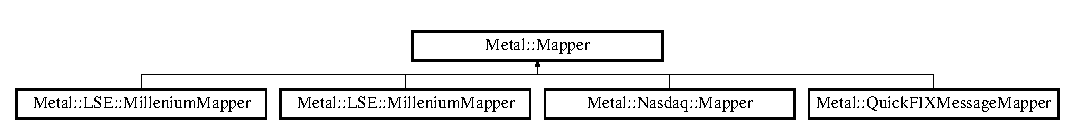
\includegraphics[height=2.000000cm]{classMetal_1_1Mapper}
\end{center}
\end{figure}


The documentation for this class was generated from the following files\+:\begin{DoxyCompactItemize}
\item 
/home/jc/metal/src/metal/Mapper.\+h\item 
/home/jc/metal/src/metal/Mapper.\+cpp\end{DoxyCompactItemize}

\hypertarget{classMetal_1_1Nasdaq_1_1Mapper}{}\section{Metal\+:\+:Nasdaq\+:\+:Mapper Class Reference}
\label{classMetal_1_1Nasdaq_1_1Mapper}\index{Metal\+::\+Nasdaq\+::\+Mapper@{Metal\+::\+Nasdaq\+::\+Mapper}}


{\ttfamily \#include $<$Mapper.\+h$>$}

Inheritance diagram for Metal\+:\+:Nasdaq\+:\+:Mapper\+:\begin{figure}[H]
\begin{center}
\leavevmode
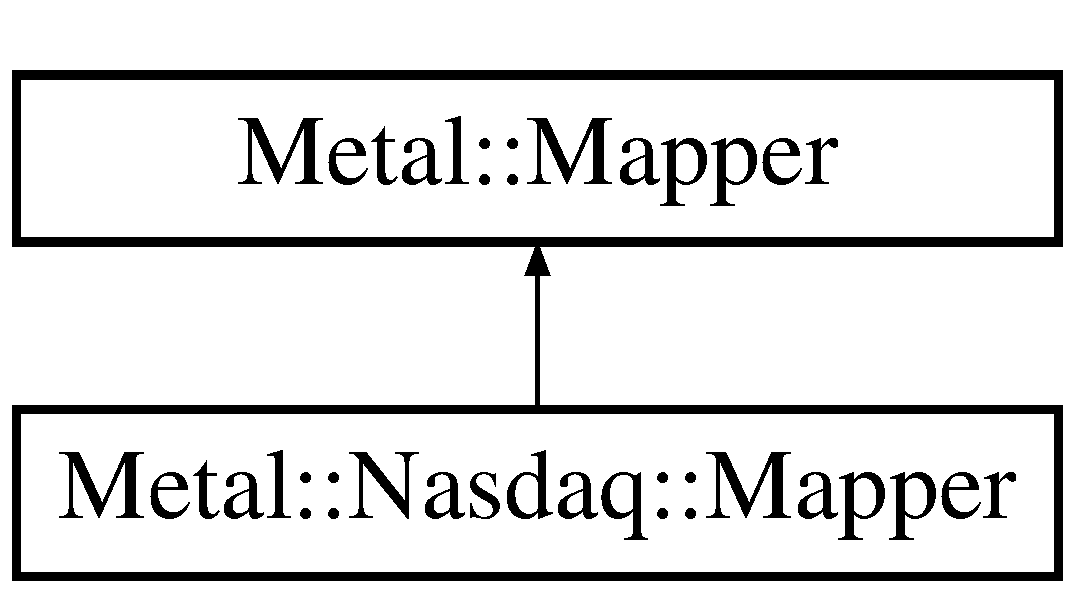
\includegraphics[height=2.000000cm]{classMetal_1_1Nasdaq_1_1Mapper}
\end{center}
\end{figure}
\subsection*{Public Attributes}
\begin{DoxyCompactItemize}
\item 
std\+::map$<$ std\+::string, std\+::string $>$ \hyperlink{classMetal_1_1Nasdaq_1_1Mapper_adc94e6a8da3f51ab0d259253eb9c4d98}{side\+From}
\end{DoxyCompactItemize}
\subsection*{Additional Inherited Members}


\subsection{Member Data Documentation}
\hypertarget{classMetal_1_1Nasdaq_1_1Mapper_adc94e6a8da3f51ab0d259253eb9c4d98}{}\index{Metal\+::\+Nasdaq\+::\+Mapper@{Metal\+::\+Nasdaq\+::\+Mapper}!side\+From@{side\+From}}
\index{side\+From@{side\+From}!Metal\+::\+Nasdaq\+::\+Mapper@{Metal\+::\+Nasdaq\+::\+Mapper}}
\subsubsection[{side\+From}]{\setlength{\rightskip}{0pt plus 5cm}std\+::map$<$std\+::string,std\+::string$>$ Metal\+::\+Nasdaq\+::\+Mapper\+::side\+From}\label{classMetal_1_1Nasdaq_1_1Mapper_adc94e6a8da3f51ab0d259253eb9c4d98}


The documentation for this class was generated from the following file\+:\begin{DoxyCompactItemize}
\item 
/home/jc/metal/github/src/adapters/\+Nasdaq\+O\+U\+C\+H-\/42/\hyperlink{src_2adapters_2NasdaqOUCH-42_2Mapper_8h}{Mapper.\+h}\end{DoxyCompactItemize}

\hypertarget{classBootstrapper_1_1MappingEntry}{}\section{Bootstrapper\+:\+:Mapping\+Entry Class Reference}
\label{classBootstrapper_1_1MappingEntry}\index{Bootstrapper\+::\+Mapping\+Entry@{Bootstrapper\+::\+Mapping\+Entry}}


{\ttfamily \#include $<$Mapping\+Table.\+h$>$}

\subsection*{Public Member Functions}
\begin{DoxyCompactItemize}
\item 
\hyperlink{classBootstrapper_1_1MappingEntry_aa98284d17f9dd3f4994a97db229b00b3}{Mapping\+Entry} (Json\+::\+Value \&entry)
\end{DoxyCompactItemize}
\subsection*{Public Attributes}
\begin{DoxyCompactItemize}
\item 
string \hyperlink{classBootstrapper_1_1MappingEntry_a65b7b8ad84053949d5213f3faedba59a}{name}
\item 
\hyperlink{unionNativeValue}{Native\+Value} \hyperlink{classBootstrapper_1_1MappingEntry_af9a9f599c7e96481c276d0a7f1589152}{native\+Value}
\item 
string \hyperlink{classBootstrapper_1_1MappingEntry_ae1c751d1bc9a672d87ec1f5ee2a267b0}{fix\+Value}
\end{DoxyCompactItemize}


\subsection{Constructor \& Destructor Documentation}
\hypertarget{classBootstrapper_1_1MappingEntry_aa98284d17f9dd3f4994a97db229b00b3}{}\index{Bootstrapper\+::\+Mapping\+Entry@{Bootstrapper\+::\+Mapping\+Entry}!Mapping\+Entry@{Mapping\+Entry}}
\index{Mapping\+Entry@{Mapping\+Entry}!Bootstrapper\+::\+Mapping\+Entry@{Bootstrapper\+::\+Mapping\+Entry}}
\subsubsection[{Mapping\+Entry}]{\setlength{\rightskip}{0pt plus 5cm}Bootstrapper\+::\+Mapping\+Entry\+::\+Mapping\+Entry (
\begin{DoxyParamCaption}
\item[{Json\+::\+Value \&}]{entry}
\end{DoxyParamCaption}
)}\label{classBootstrapper_1_1MappingEntry_aa98284d17f9dd3f4994a97db229b00b3}


\subsection{Member Data Documentation}
\hypertarget{classBootstrapper_1_1MappingEntry_ae1c751d1bc9a672d87ec1f5ee2a267b0}{}\index{Bootstrapper\+::\+Mapping\+Entry@{Bootstrapper\+::\+Mapping\+Entry}!fix\+Value@{fix\+Value}}
\index{fix\+Value@{fix\+Value}!Bootstrapper\+::\+Mapping\+Entry@{Bootstrapper\+::\+Mapping\+Entry}}
\subsubsection[{fix\+Value}]{\setlength{\rightskip}{0pt plus 5cm}string Bootstrapper\+::\+Mapping\+Entry\+::fix\+Value}\label{classBootstrapper_1_1MappingEntry_ae1c751d1bc9a672d87ec1f5ee2a267b0}
\hypertarget{classBootstrapper_1_1MappingEntry_a65b7b8ad84053949d5213f3faedba59a}{}\index{Bootstrapper\+::\+Mapping\+Entry@{Bootstrapper\+::\+Mapping\+Entry}!name@{name}}
\index{name@{name}!Bootstrapper\+::\+Mapping\+Entry@{Bootstrapper\+::\+Mapping\+Entry}}
\subsubsection[{name}]{\setlength{\rightskip}{0pt plus 5cm}string Bootstrapper\+::\+Mapping\+Entry\+::name}\label{classBootstrapper_1_1MappingEntry_a65b7b8ad84053949d5213f3faedba59a}
\hypertarget{classBootstrapper_1_1MappingEntry_af9a9f599c7e96481c276d0a7f1589152}{}\index{Bootstrapper\+::\+Mapping\+Entry@{Bootstrapper\+::\+Mapping\+Entry}!native\+Value@{native\+Value}}
\index{native\+Value@{native\+Value}!Bootstrapper\+::\+Mapping\+Entry@{Bootstrapper\+::\+Mapping\+Entry}}
\subsubsection[{native\+Value}]{\setlength{\rightskip}{0pt plus 5cm}{\bf Native\+Value} Bootstrapper\+::\+Mapping\+Entry\+::native\+Value}\label{classBootstrapper_1_1MappingEntry_af9a9f599c7e96481c276d0a7f1589152}


The documentation for this class was generated from the following files\+:\begin{DoxyCompactItemize}
\item 
/home/jc/metal/github/src/bootstrapper/\hyperlink{MappingTable_8h}{Mapping\+Table.\+h}\item 
/home/jc/metal/github/src/bootstrapper/\hyperlink{MappingTable_8cpp}{Mapping\+Table.\+cpp}\end{DoxyCompactItemize}

\hypertarget{classMetal_1_1MappingException}{}\section{Metal\+:\+:Mapping\+Exception Class Reference}
\label{classMetal_1_1MappingException}\index{Metal\+::\+Mapping\+Exception@{Metal\+::\+Mapping\+Exception}}
Inheritance diagram for Metal\+:\+:Mapping\+Exception\+:\begin{figure}[H]
\begin{center}
\leavevmode
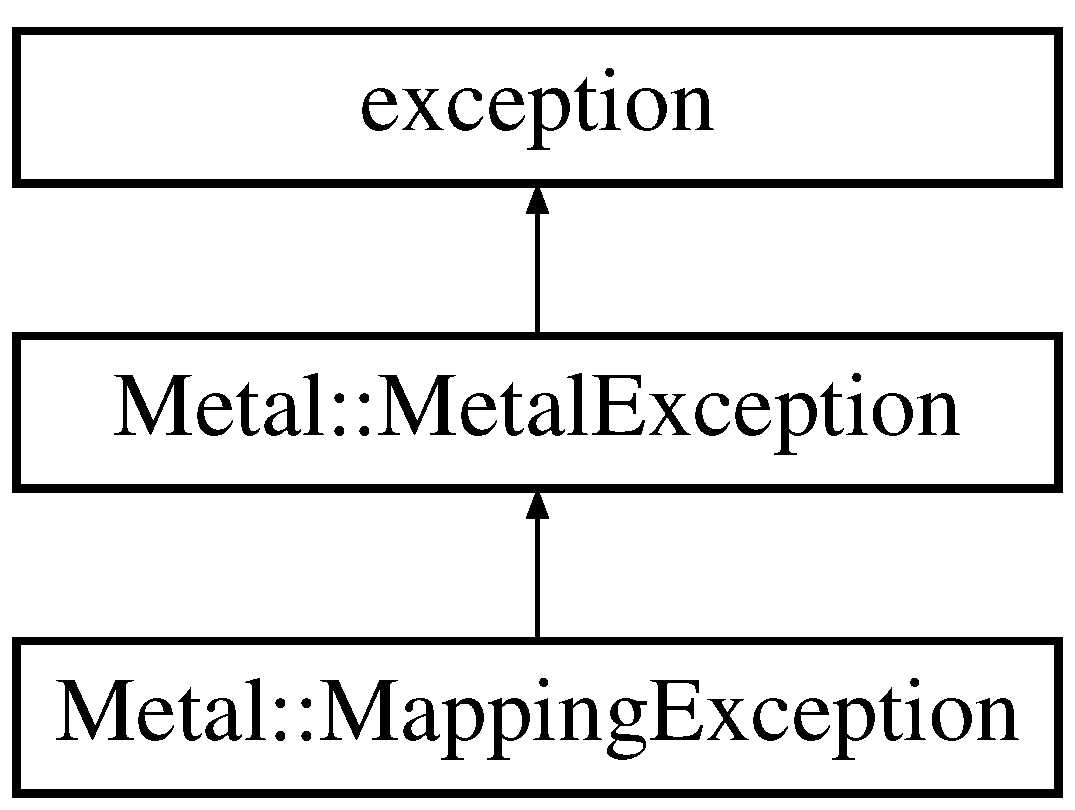
\includegraphics[height=3.000000cm]{classMetal_1_1MappingException}
\end{center}
\end{figure}
\subsection*{Public Member Functions}
\begin{DoxyCompactItemize}
\item 
\hypertarget{classMetal_1_1MappingException_ac343b35119e5515197df087da5fceeaf}{}{\bfseries Mapping\+Exception} (const std\+::string \&message)\label{classMetal_1_1MappingException_ac343b35119e5515197df087da5fceeaf}

\end{DoxyCompactItemize}


The documentation for this class was generated from the following file\+:\begin{DoxyCompactItemize}
\item 
/home/jc/metal/src/metal/Metal\+Exceptions.\+h\end{DoxyCompactItemize}

\hypertarget{classBootstrapper_1_1MappingTable}{}\section{Bootstrapper\+:\+:Mapping\+Table Class Reference}
\label{classBootstrapper_1_1MappingTable}\index{Bootstrapper\+::\+Mapping\+Table@{Bootstrapper\+::\+Mapping\+Table}}


{\ttfamily \#include $<$Mapping\+Table.\+h$>$}

\subsection*{Public Member Functions}
\begin{DoxyCompactItemize}
\item 
\hyperlink{classBootstrapper_1_1MappingTable_a8f7cb038c10f3123e0e29db7a974e29e}{Mapping\+Table} (Json\+::\+Value source)
\item 
\hyperlink{classBootstrapper_1_1MappingTable_a62950403dec2606ce8772c8305b006ed}{$\sim$\+Mapping\+Table} ()
\item 
void \hyperlink{classBootstrapper_1_1MappingTable_a81e665f9c02b9534720317e95743e1c9}{add\+Declaration} (stringstream \&ss)
\item 
void \hyperlink{classBootstrapper_1_1MappingTable_a2ab120f2cb5ed1dc93159ddc55264f19}{add\+Initialization} (stringstream \&ss)
\end{DoxyCompactItemize}
\subsection*{Public Attributes}
\begin{DoxyCompactItemize}
\item 
std\+::string \hyperlink{classBootstrapper_1_1MappingTable_aa1b11e86b77f9514cb067f6bf9ab5ef1}{name}
\item 
std\+::vector$<$ \hyperlink{classBootstrapper_1_1MappingEntry}{Mapping\+Entry} $\ast$ $>$ \hyperlink{classBootstrapper_1_1MappingTable_ad60b5c92cc19d1d31ed8012c22946fee}{values}
\item 
\hyperlink{namespaceBootstrapper_abb268c54c14e352b0204f5f0f928955f}{Field\+Type} \hyperlink{classBootstrapper_1_1MappingTable_aa433179b2b5409ee43d726554f260879}{field\+Type}
\end{DoxyCompactItemize}


\subsection{Constructor \& Destructor Documentation}
\hypertarget{classBootstrapper_1_1MappingTable_a8f7cb038c10f3123e0e29db7a974e29e}{}\index{Bootstrapper\+::\+Mapping\+Table@{Bootstrapper\+::\+Mapping\+Table}!Mapping\+Table@{Mapping\+Table}}
\index{Mapping\+Table@{Mapping\+Table}!Bootstrapper\+::\+Mapping\+Table@{Bootstrapper\+::\+Mapping\+Table}}
\subsubsection[{Mapping\+Table}]{\setlength{\rightskip}{0pt plus 5cm}Bootstrapper\+::\+Mapping\+Table\+::\+Mapping\+Table (
\begin{DoxyParamCaption}
\item[{Json\+::\+Value}]{source}
\end{DoxyParamCaption}
)}\label{classBootstrapper_1_1MappingTable_a8f7cb038c10f3123e0e29db7a974e29e}
May throw an exception if the inbound json is incorretly formatted \hypertarget{classBootstrapper_1_1MappingTable_a62950403dec2606ce8772c8305b006ed}{}\index{Bootstrapper\+::\+Mapping\+Table@{Bootstrapper\+::\+Mapping\+Table}!````~Mapping\+Table@{$\sim$\+Mapping\+Table}}
\index{````~Mapping\+Table@{$\sim$\+Mapping\+Table}!Bootstrapper\+::\+Mapping\+Table@{Bootstrapper\+::\+Mapping\+Table}}
\subsubsection[{$\sim$\+Mapping\+Table}]{\setlength{\rightskip}{0pt plus 5cm}Bootstrapper\+::\+Mapping\+Table\+::$\sim$\+Mapping\+Table (
\begin{DoxyParamCaption}
{}
\end{DoxyParamCaption}
)}\label{classBootstrapper_1_1MappingTable_a62950403dec2606ce8772c8305b006ed}


\subsection{Member Function Documentation}
\hypertarget{classBootstrapper_1_1MappingTable_a81e665f9c02b9534720317e95743e1c9}{}\index{Bootstrapper\+::\+Mapping\+Table@{Bootstrapper\+::\+Mapping\+Table}!add\+Declaration@{add\+Declaration}}
\index{add\+Declaration@{add\+Declaration}!Bootstrapper\+::\+Mapping\+Table@{Bootstrapper\+::\+Mapping\+Table}}
\subsubsection[{add\+Declaration}]{\setlength{\rightskip}{0pt plus 5cm}void Bootstrapper\+::\+Mapping\+Table\+::add\+Declaration (
\begin{DoxyParamCaption}
\item[{stringstream \&}]{ss}
\end{DoxyParamCaption}
)}\label{classBootstrapper_1_1MappingTable_a81e665f9c02b9534720317e95743e1c9}
\hypertarget{classBootstrapper_1_1MappingTable_a2ab120f2cb5ed1dc93159ddc55264f19}{}\index{Bootstrapper\+::\+Mapping\+Table@{Bootstrapper\+::\+Mapping\+Table}!add\+Initialization@{add\+Initialization}}
\index{add\+Initialization@{add\+Initialization}!Bootstrapper\+::\+Mapping\+Table@{Bootstrapper\+::\+Mapping\+Table}}
\subsubsection[{add\+Initialization}]{\setlength{\rightskip}{0pt plus 5cm}void Bootstrapper\+::\+Mapping\+Table\+::add\+Initialization (
\begin{DoxyParamCaption}
\item[{stringstream \&}]{ss}
\end{DoxyParamCaption}
)}\label{classBootstrapper_1_1MappingTable_a2ab120f2cb5ed1dc93159ddc55264f19}
Format initialization source code 
\begin{DoxyParams}{Parameters}
{\em ss} & output stringstream where source code will be appended \\
\hline
\end{DoxyParams}


\subsection{Member Data Documentation}
\hypertarget{classBootstrapper_1_1MappingTable_aa433179b2b5409ee43d726554f260879}{}\index{Bootstrapper\+::\+Mapping\+Table@{Bootstrapper\+::\+Mapping\+Table}!field\+Type@{field\+Type}}
\index{field\+Type@{field\+Type}!Bootstrapper\+::\+Mapping\+Table@{Bootstrapper\+::\+Mapping\+Table}}
\subsubsection[{field\+Type}]{\setlength{\rightskip}{0pt plus 5cm}{\bf Field\+Type} Bootstrapper\+::\+Mapping\+Table\+::field\+Type}\label{classBootstrapper_1_1MappingTable_aa433179b2b5409ee43d726554f260879}
\hypertarget{classBootstrapper_1_1MappingTable_aa1b11e86b77f9514cb067f6bf9ab5ef1}{}\index{Bootstrapper\+::\+Mapping\+Table@{Bootstrapper\+::\+Mapping\+Table}!name@{name}}
\index{name@{name}!Bootstrapper\+::\+Mapping\+Table@{Bootstrapper\+::\+Mapping\+Table}}
\subsubsection[{name}]{\setlength{\rightskip}{0pt plus 5cm}std\+::string Bootstrapper\+::\+Mapping\+Table\+::name}\label{classBootstrapper_1_1MappingTable_aa1b11e86b77f9514cb067f6bf9ab5ef1}
\hypertarget{classBootstrapper_1_1MappingTable_ad60b5c92cc19d1d31ed8012c22946fee}{}\index{Bootstrapper\+::\+Mapping\+Table@{Bootstrapper\+::\+Mapping\+Table}!values@{values}}
\index{values@{values}!Bootstrapper\+::\+Mapping\+Table@{Bootstrapper\+::\+Mapping\+Table}}
\subsubsection[{values}]{\setlength{\rightskip}{0pt plus 5cm}std\+::vector$<${\bf Mapping\+Entry}$\ast$$>$ Bootstrapper\+::\+Mapping\+Table\+::values}\label{classBootstrapper_1_1MappingTable_ad60b5c92cc19d1d31ed8012c22946fee}


The documentation for this class was generated from the following files\+:\begin{DoxyCompactItemize}
\item 
/home/jc/metal/github/src/bootstrapper/\hyperlink{MappingTable_8h}{Mapping\+Table.\+h}\item 
/home/jc/metal/github/src/bootstrapper/\hyperlink{MappingTable_8cpp}{Mapping\+Table.\+cpp}\end{DoxyCompactItemize}

\hypertarget{classMetal_1_1Message}{}\section{Metal\+:\+:Message Class Reference}
\label{classMetal_1_1Message}\index{Metal\+::\+Message@{Metal\+::\+Message}}
\subsection*{Public Member Functions}
\begin{DoxyCompactItemize}
\item 
\hypertarget{classMetal_1_1Message_abc94615951dbde67368f977b717176fe}{}const char $\ast$ {\bfseries get\+Data} ()\label{classMetal_1_1Message_abc94615951dbde67368f977b717176fe}

\item 
\hypertarget{classMetal_1_1Message_a22984c81035306cfde91a575ac19d32a}{}const size\+\_\+t {\bfseries get\+Length} ()\label{classMetal_1_1Message_a22984c81035306cfde91a575ac19d32a}

\item 
void \hyperlink{classMetal_1_1Message_a9f9b7fb98dbe697d9cf7ad394fd45a2e}{set} (int position, char value)
\item 
void \hyperlink{classMetal_1_1Message_a7cb33179723ecc8a05860a97d9a518e3}{set} (int position, std\+::string str, int max\+Length)
\end{DoxyCompactItemize}


\subsection{Member Function Documentation}
\hypertarget{classMetal_1_1Message_a9f9b7fb98dbe697d9cf7ad394fd45a2e}{}\index{Metal\+::\+Message@{Metal\+::\+Message}!set@{set}}
\index{set@{set}!Metal\+::\+Message@{Metal\+::\+Message}}
\subsubsection[{set}]{\setlength{\rightskip}{0pt plus 5cm}void Metal\+::\+Message\+::set (
\begin{DoxyParamCaption}
\item[{int}]{position, }
\item[{char}]{value}
\end{DoxyParamCaption}
)\hspace{0.3cm}{\ttfamily [inline]}}\label{classMetal_1_1Message_a9f9b7fb98dbe697d9cf7ad394fd45a2e}
Write a single character at given position 
\begin{DoxyParams}{Parameters}
{\em position} & Where the character should be writted \\
\hline
{\em value} & Value to be written \\
\hline
\end{DoxyParams}
\hypertarget{classMetal_1_1Message_a7cb33179723ecc8a05860a97d9a518e3}{}\index{Metal\+::\+Message@{Metal\+::\+Message}!set@{set}}
\index{set@{set}!Metal\+::\+Message@{Metal\+::\+Message}}
\subsubsection[{set}]{\setlength{\rightskip}{0pt plus 5cm}void Metal\+::\+Message\+::set (
\begin{DoxyParamCaption}
\item[{int}]{position, }
\item[{std\+::string}]{str, }
\item[{int}]{max\+Length}
\end{DoxyParamCaption}
)\hspace{0.3cm}{\ttfamily [inline]}}\label{classMetal_1_1Message_a7cb33179723ecc8a05860a97d9a518e3}
Write a complete string at given position 
\begin{DoxyParams}{Parameters}
{\em position} & Where the string should be writted \\
\hline
{\em str} & String to be written \\
\hline
{\em max\+Length} & maximum length to be copied from the string \\
\hline
\end{DoxyParams}


The documentation for this class was generated from the following files\+:\begin{DoxyCompactItemize}
\item 
/home/jc/metal/src/metal/Message.\+h\item 
/home/jc/metal/src/metal/Message.\+cpp\end{DoxyCompactItemize}

\hypertarget{classMetal_1_1MetalException}{}\section{Metal\+:\+:Metal\+Exception Class Reference}
\label{classMetal_1_1MetalException}\index{Metal\+::\+Metal\+Exception@{Metal\+::\+Metal\+Exception}}
Inheritance diagram for Metal\+:\+:Metal\+Exception\+:\begin{figure}[H]
\begin{center}
\leavevmode
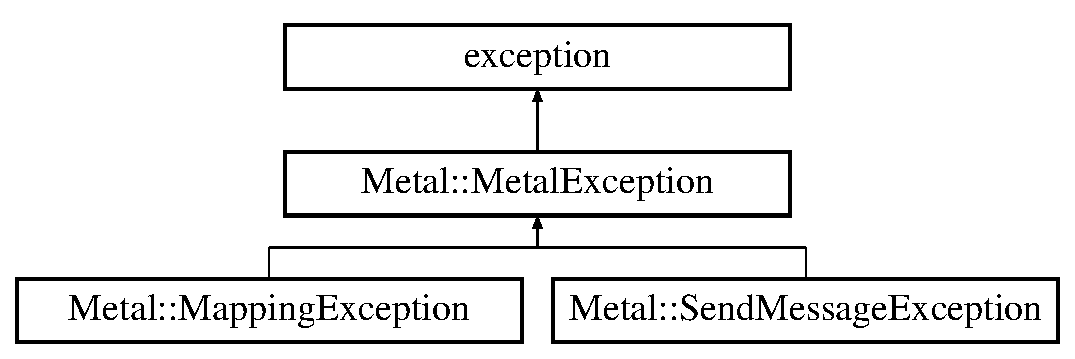
\includegraphics[height=3.000000cm]{classMetal_1_1MetalException}
\end{center}
\end{figure}
\subsection*{Public Member Functions}
\begin{DoxyCompactItemize}
\item 
\hypertarget{classMetal_1_1MetalException_afa58e4cd82c3aca7a138024fd1b6f090}{}{\bfseries Metal\+Exception} (const std\+::string \&message)\label{classMetal_1_1MetalException_afa58e4cd82c3aca7a138024fd1b6f090}

\item 
\hypertarget{classMetal_1_1MetalException_a74fa237bd4484764faccfbebd54801b5}{}virtual const char $\ast$ {\bfseries what} () const   throw ()\label{classMetal_1_1MetalException_a74fa237bd4484764faccfbebd54801b5}

\end{DoxyCompactItemize}


The documentation for this class was generated from the following file\+:\begin{DoxyCompactItemize}
\item 
/home/jc/metal/src/metal/Metal\+Exceptions.\+h\end{DoxyCompactItemize}

\hypertarget{classMetal_1_1LSE_1_1MilleniumAdapter}{}\section{Metal\+:\+:L\+S\+E\+:\+:Millenium\+Adapter Class Reference}
\label{classMetal_1_1LSE_1_1MilleniumAdapter}\index{Metal\+::\+L\+S\+E\+::\+Millenium\+Adapter@{Metal\+::\+L\+S\+E\+::\+Millenium\+Adapter}}
Inheritance diagram for Metal\+:\+:L\+S\+E\+:\+:Millenium\+Adapter\+:\begin{figure}[H]
\begin{center}
\leavevmode
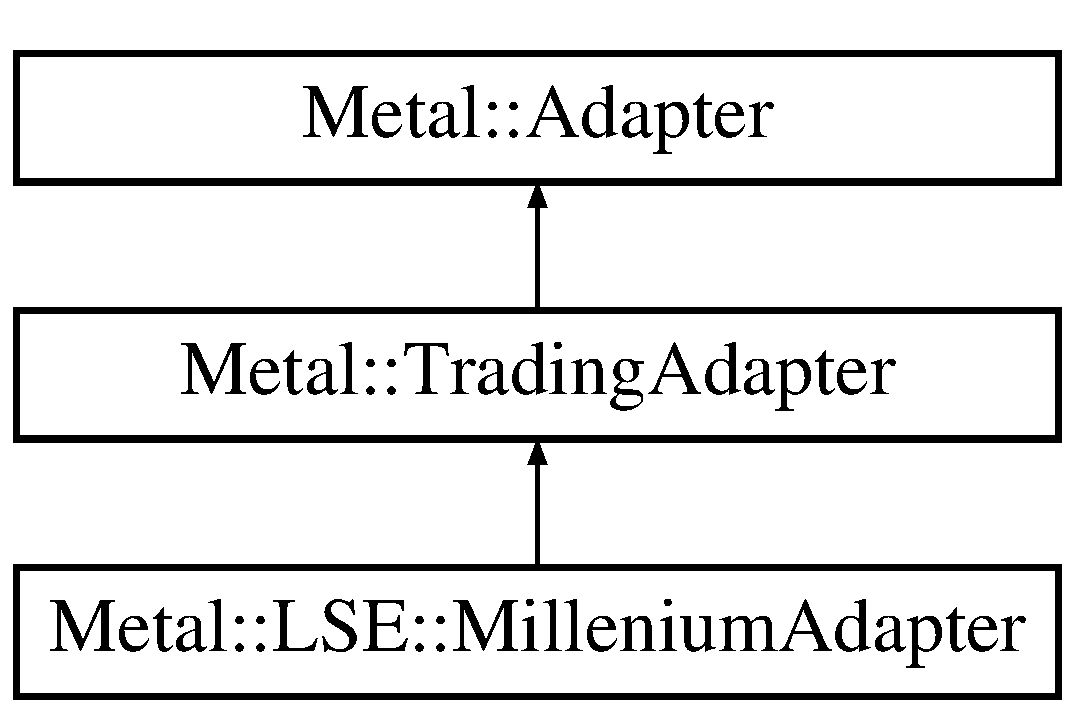
\includegraphics[height=3.000000cm]{classMetal_1_1LSE_1_1MilleniumAdapter}
\end{center}
\end{figure}
\subsection*{Public Member Functions}
\begin{DoxyCompactItemize}
\item 
void \hyperlink{classMetal_1_1LSE_1_1MilleniumAdapter_ab3da43142636043e0ade20b0881c9976}{send} (const \hyperlink{classMetal_1_1NewOrderSingle}{New\+Order\+Single} \&nos)
\item 
virtual void \hyperlink{classMetal_1_1LSE_1_1MilleniumAdapter_add4508b367a6383b42fb2fd1744946cd}{recv} (const Execution\+Report \&er)
\item 
\hypertarget{classMetal_1_1LSE_1_1MilleniumAdapter_a402c564b7a955fac6660e6bfeee66093}{}void {\bfseries start} ()\label{classMetal_1_1LSE_1_1MilleniumAdapter_a402c564b7a955fac6660e6bfeee66093}

\item 
\hypertarget{classMetal_1_1LSE_1_1MilleniumAdapter_acb5018d36915f34612958d87ad8325af}{}void {\bfseries stop} ()\label{classMetal_1_1LSE_1_1MilleniumAdapter_acb5018d36915f34612958d87ad8325af}

\item 
void \hyperlink{classMetal_1_1LSE_1_1MilleniumAdapter_ab4bba2e8403ae7ed5b335985b4295b9f}{send\+Logon} ()
\item 
void \hyperlink{classMetal_1_1LSE_1_1MilleniumAdapter_a01a0796b972925d6a430e2f788eec5ee}{benchmark} (const std\+::vector$<$ \hyperlink{classMetal_1_1NewOrderSingle}{Metal\+::\+New\+Order\+Single} $>$ \&, std\+::chrono\+::milliseconds \&mapping\+Duration, std\+::chrono\+::milliseconds \&encoding\+Duration)
\item 
void \hyperlink{classMetal_1_1LSE_1_1MilleniumAdapter_acdfc9b84439e745de42c0f72a1e22a67}{benchmark} (const std\+::vector$<$ \hyperlink{classMetal_1_1OrderCancelRequest}{Metal\+::\+Order\+Cancel\+Request} $>$ \&, std\+::chrono\+::milliseconds \&, std\+::chrono\+::milliseconds \&)
\end{DoxyCompactItemize}
\subsection*{Protected Attributes}
\begin{DoxyCompactItemize}
\item 
\hypertarget{classMetal_1_1LSE_1_1MilleniumAdapter_a1c12122da30ec79f3907a82ac1847c33}{}std\+::string {\bfseries user\+Name}\label{classMetal_1_1LSE_1_1MilleniumAdapter_a1c12122da30ec79f3907a82ac1847c33}

\item 
\hypertarget{classMetal_1_1LSE_1_1MilleniumAdapter_aa8120f11aac5d4825a5766d86e53e5a2}{}std\+::string {\bfseries password}\label{classMetal_1_1LSE_1_1MilleniumAdapter_aa8120f11aac5d4825a5766d86e53e5a2}

\end{DoxyCompactItemize}
\subsection*{Additional Inherited Members}


\subsection{Member Function Documentation}
\hypertarget{classMetal_1_1LSE_1_1MilleniumAdapter_a01a0796b972925d6a430e2f788eec5ee}{}\index{Metal\+::\+L\+S\+E\+::\+Millenium\+Adapter@{Metal\+::\+L\+S\+E\+::\+Millenium\+Adapter}!benchmark@{benchmark}}
\index{benchmark@{benchmark}!Metal\+::\+L\+S\+E\+::\+Millenium\+Adapter@{Metal\+::\+L\+S\+E\+::\+Millenium\+Adapter}}
\subsubsection[{benchmark}]{\setlength{\rightskip}{0pt plus 5cm}void Metal\+::\+L\+S\+E\+::\+Millenium\+Adapter\+::benchmark (
\begin{DoxyParamCaption}
\item[{const std\+::vector$<$ {\bf Metal\+::\+New\+Order\+Single} $>$ \&}]{, }
\item[{std\+::chrono\+::milliseconds \&}]{mapping\+Duration, }
\item[{std\+::chrono\+::milliseconds \&}]{encoding\+Duration}
\end{DoxyParamCaption}
)}\label{classMetal_1_1LSE_1_1MilleniumAdapter_a01a0796b972925d6a430e2f788eec5ee}
\begin{DoxySeeAlso}{See also}
\hyperlink{classMetal_1_1TradingAdapter_a161ad3db17091807d091d1b236de0105}{Trading\+Adapter\+::benchmark} 
\end{DoxySeeAlso}
\hypertarget{classMetal_1_1LSE_1_1MilleniumAdapter_acdfc9b84439e745de42c0f72a1e22a67}{}\index{Metal\+::\+L\+S\+E\+::\+Millenium\+Adapter@{Metal\+::\+L\+S\+E\+::\+Millenium\+Adapter}!benchmark@{benchmark}}
\index{benchmark@{benchmark}!Metal\+::\+L\+S\+E\+::\+Millenium\+Adapter@{Metal\+::\+L\+S\+E\+::\+Millenium\+Adapter}}
\subsubsection[{benchmark}]{\setlength{\rightskip}{0pt plus 5cm}void Metal\+::\+L\+S\+E\+::\+Millenium\+Adapter\+::benchmark (
\begin{DoxyParamCaption}
\item[{const std\+::vector$<$ {\bf Metal\+::\+Order\+Cancel\+Request} $>$ \&}]{all\+Cancels, }
\item[{std\+::chrono\+::milliseconds \&}]{mapping\+Duration, }
\item[{std\+::chrono\+::milliseconds \&}]{encoding\+Duration}
\end{DoxyParamCaption}
)}\label{classMetal_1_1LSE_1_1MilleniumAdapter_acdfc9b84439e745de42c0f72a1e22a67}
\begin{DoxySeeAlso}{See also}
\hyperlink{classMetal_1_1TradingAdapter_a161ad3db17091807d091d1b236de0105}{Trading\+Adapter\+::benchmark} 
\end{DoxySeeAlso}
\hypertarget{classMetal_1_1LSE_1_1MilleniumAdapter_add4508b367a6383b42fb2fd1744946cd}{}\index{Metal\+::\+L\+S\+E\+::\+Millenium\+Adapter@{Metal\+::\+L\+S\+E\+::\+Millenium\+Adapter}!recv@{recv}}
\index{recv@{recv}!Metal\+::\+L\+S\+E\+::\+Millenium\+Adapter@{Metal\+::\+L\+S\+E\+::\+Millenium\+Adapter}}
\subsubsection[{recv}]{\setlength{\rightskip}{0pt plus 5cm}void Metal\+::\+L\+S\+E\+::\+Millenium\+Adapter\+::recv (
\begin{DoxyParamCaption}
\item[{const Execution\+Report \&}]{er}
\end{DoxyParamCaption}
)\hspace{0.3cm}{\ttfamily [virtual]}}\label{classMetal_1_1LSE_1_1MilleniumAdapter_add4508b367a6383b42fb2fd1744946cd}
This method will invoked upon receiving an execution report~\newline
 Subclasses will perform mapping, encoding then write to the active session~\newline
 
\begin{DoxyParams}{Parameters}
{\em Execution\+Report} & incomming execution report \\
\hline
\end{DoxyParams}


Implements \hyperlink{classMetal_1_1TradingAdapter_af0015d51815dedb1bc78258b3030d751}{Metal\+::\+Trading\+Adapter}.

\hypertarget{classMetal_1_1LSE_1_1MilleniumAdapter_ab3da43142636043e0ade20b0881c9976}{}\index{Metal\+::\+L\+S\+E\+::\+Millenium\+Adapter@{Metal\+::\+L\+S\+E\+::\+Millenium\+Adapter}!send@{send}}
\index{send@{send}!Metal\+::\+L\+S\+E\+::\+Millenium\+Adapter@{Metal\+::\+L\+S\+E\+::\+Millenium\+Adapter}}
\subsubsection[{send}]{\setlength{\rightskip}{0pt plus 5cm}void Metal\+::\+L\+S\+E\+::\+Millenium\+Adapter\+::send (
\begin{DoxyParamCaption}
\item[{const {\bf New\+Order\+Single} \&}]{}
\end{DoxyParamCaption}
)\hspace{0.3cm}{\ttfamily [virtual]}}\label{classMetal_1_1LSE_1_1MilleniumAdapter_ab3da43142636043e0ade20b0881c9976}
This method will be called by users to send new orders~\newline
 Subclasses will perform mapping, encoding then write to the active session~\newline
 
\begin{DoxyParams}{Parameters}
{\em \hyperlink{classMetal_1_1NewOrderSingle}{New\+Order\+Single}} & Inbound order in unified format \\
\hline
\end{DoxyParams}
\begin{DoxySeeAlso}{See also}
\hyperlink{classMetal_1_1NewOrderSingle}{New\+Order\+Single} 
\end{DoxySeeAlso}


Implements \hyperlink{classMetal_1_1TradingAdapter_a2ecc8f1c8fe8a8d29625d142f473f1c3}{Metal\+::\+Trading\+Adapter}.

\hypertarget{classMetal_1_1LSE_1_1MilleniumAdapter_ab4bba2e8403ae7ed5b335985b4295b9f}{}\index{Metal\+::\+L\+S\+E\+::\+Millenium\+Adapter@{Metal\+::\+L\+S\+E\+::\+Millenium\+Adapter}!send\+Logon@{send\+Logon}}
\index{send\+Logon@{send\+Logon}!Metal\+::\+L\+S\+E\+::\+Millenium\+Adapter@{Metal\+::\+L\+S\+E\+::\+Millenium\+Adapter}}
\subsubsection[{send\+Logon}]{\setlength{\rightskip}{0pt plus 5cm}void Metal\+::\+L\+S\+E\+::\+Millenium\+Adapter\+::send\+Logon (
\begin{DoxyParamCaption}
{}
\end{DoxyParamCaption}
)\hspace{0.3cm}{\ttfamily [virtual]}}\label{classMetal_1_1LSE_1_1MilleniumAdapter_ab4bba2e8403ae7ed5b335985b4295b9f}
This pure virtual method should be implemented in each adapter. 

Implements \hyperlink{classMetal_1_1TradingAdapter_a39562015df3e7202a5e8f932b8bde43e}{Metal\+::\+Trading\+Adapter}.



The documentation for this class was generated from the following files\+:\begin{DoxyCompactItemize}
\item 
/home/jc/metal/src/metal/adapters/\+L\+S\+E\+Trading\+Adapter/Millenium\+Adapter.\+h\item 
/home/jc/metal/src/metal/adapters/\+L\+S\+E\+Trading\+Adapter/Millenium\+Adapter.\+cpp\end{DoxyCompactItemize}

\hypertarget{classMetal_1_1LSE_1_1MilleniumCodec}{}\section{Metal\+:\+:L\+S\+E\+:\+:Millenium\+Codec Class Reference}
\label{classMetal_1_1LSE_1_1MilleniumCodec}\index{Metal\+::\+L\+S\+E\+::\+Millenium\+Codec@{Metal\+::\+L\+S\+E\+::\+Millenium\+Codec}}
Inheritance diagram for Metal\+:\+:L\+S\+E\+:\+:Millenium\+Codec\+:\begin{figure}[H]
\begin{center}
\leavevmode
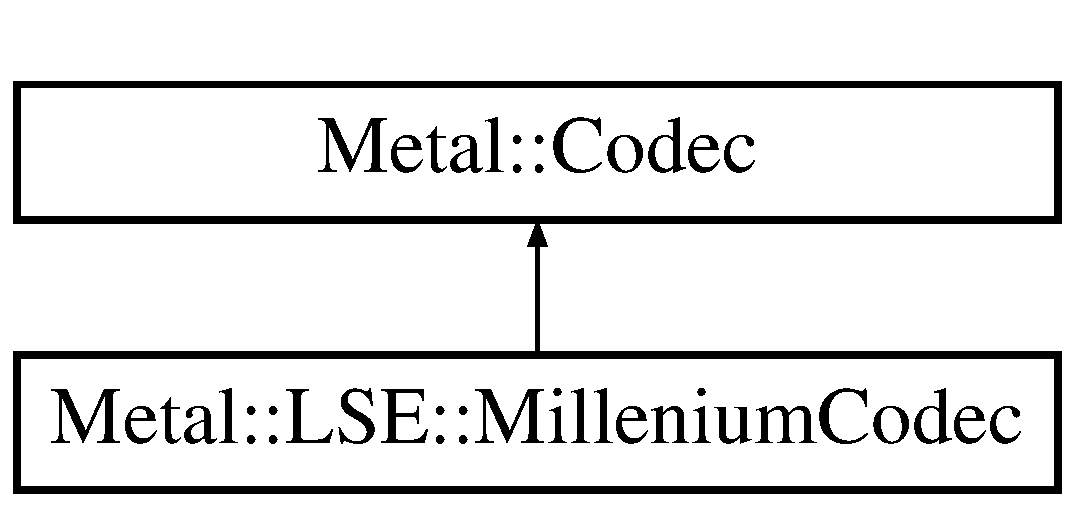
\includegraphics[height=2.000000cm]{classMetal_1_1LSE_1_1MilleniumCodec}
\end{center}
\end{figure}
\subsection*{Static Public Member Functions}
\begin{DoxyCompactItemize}
\item 
static void \hyperlink{classMetal_1_1LSE_1_1MilleniumCodec_a0db727988a60b489983d3650c2dbb5fd}{encode} (const \hyperlink{classMetal_1_1LSE_1_1OrderCancelRequest}{Order\+Cancel\+Request} \&ocr, \hyperlink{classMetal_1_1Message}{Message} \&msg)
\item 
static void \hyperlink{classMetal_1_1LSE_1_1MilleniumCodec_a90425eb0c5be795fb6c35fc28a88aac1}{encode} (const \hyperlink{classMetal_1_1LSE_1_1NewOrder}{New\+Order} \&no, \hyperlink{classMetal_1_1Message}{Message} \&msg)
\item 
static void \hyperlink{classMetal_1_1LSE_1_1MilleniumCodec_a2ae620b4b54cf5dc12df16b976af4d34}{encode} (const \hyperlink{classMetal_1_1LSE_1_1Logon}{Logon} \&logon, \hyperlink{classMetal_1_1Message}{Message} \&msg)
\item 
\hypertarget{classMetal_1_1LSE_1_1MilleniumCodec_a343c554002e86b3376c160ef5aa434d1}{}static void {\bfseries encode} (const int16\+\_\+t \&i, \hyperlink{classMetal_1_1Message}{Message} \&msg, int position)\label{classMetal_1_1LSE_1_1MilleniumCodec_a343c554002e86b3376c160ef5aa434d1}

\item 
\hypertarget{classMetal_1_1LSE_1_1MilleniumCodec_a7c950822487d09fde69d98224aa95442}{}static void {\bfseries encode} (const int32\+\_\+t \&i, \hyperlink{classMetal_1_1Message}{Message} \&msg, int position)\label{classMetal_1_1LSE_1_1MilleniumCodec_a7c950822487d09fde69d98224aa95442}

\item 
\hypertarget{classMetal_1_1LSE_1_1MilleniumCodec_a1b1d14237dd5a548b59a0a3773fbee79}{}static void {\bfseries encode} (const int64\+\_\+t \&i, \hyperlink{classMetal_1_1Message}{Message} \&msg, int position)\label{classMetal_1_1LSE_1_1MilleniumCodec_a1b1d14237dd5a548b59a0a3773fbee79}

\item 
\hypertarget{classMetal_1_1LSE_1_1MilleniumCodec_a3b494f4615faf56115c32db1c3fcf4c5}{}static void {\bfseries encode\+Header} (\hyperlink{classMetal_1_1Message}{Message} \&msg, int16\+\_\+t length, char type)\label{classMetal_1_1LSE_1_1MilleniumCodec_a3b494f4615faf56115c32db1c3fcf4c5}

\end{DoxyCompactItemize}


\subsection{Member Function Documentation}
\hypertarget{classMetal_1_1LSE_1_1MilleniumCodec_a0db727988a60b489983d3650c2dbb5fd}{}\index{Metal\+::\+L\+S\+E\+::\+Millenium\+Codec@{Metal\+::\+L\+S\+E\+::\+Millenium\+Codec}!encode@{encode}}
\index{encode@{encode}!Metal\+::\+L\+S\+E\+::\+Millenium\+Codec@{Metal\+::\+L\+S\+E\+::\+Millenium\+Codec}}
\subsubsection[{encode}]{\setlength{\rightskip}{0pt plus 5cm}void Metal\+::\+L\+S\+E\+::\+Millenium\+Codec\+::encode (
\begin{DoxyParamCaption}
\item[{const {\bf Order\+Cancel\+Request} \&}]{ocr, }
\item[{{\bf Metal\+::\+Message} \&}]{msg}
\end{DoxyParamCaption}
)\hspace{0.3cm}{\ttfamily [static]}}\label{classMetal_1_1LSE_1_1MilleniumCodec_a0db727988a60b489983d3650c2dbb5fd}
Encode a cancel request 
\begin{DoxyParams}{Parameters}
{\em ocr} & The Order Cancel Request representation \\
\hline
{\em msg} & The destination message \\
\hline
\end{DoxyParams}
\hypertarget{classMetal_1_1LSE_1_1MilleniumCodec_a90425eb0c5be795fb6c35fc28a88aac1}{}\index{Metal\+::\+L\+S\+E\+::\+Millenium\+Codec@{Metal\+::\+L\+S\+E\+::\+Millenium\+Codec}!encode@{encode}}
\index{encode@{encode}!Metal\+::\+L\+S\+E\+::\+Millenium\+Codec@{Metal\+::\+L\+S\+E\+::\+Millenium\+Codec}}
\subsubsection[{encode}]{\setlength{\rightskip}{0pt plus 5cm}void Metal\+::\+L\+S\+E\+::\+Millenium\+Codec\+::encode (
\begin{DoxyParamCaption}
\item[{const {\bf New\+Order} \&}]{no, }
\item[{{\bf Metal\+::\+Message} \&}]{msg}
\end{DoxyParamCaption}
)\hspace{0.3cm}{\ttfamily [static]}}\label{classMetal_1_1LSE_1_1MilleniumCodec_a90425eb0c5be795fb6c35fc28a88aac1}
Encode a new order 
\begin{DoxyParams}{Parameters}
{\em no} & The New Order representation \\
\hline
{\em msg} & The destination message \\
\hline
\end{DoxyParams}
\hypertarget{classMetal_1_1LSE_1_1MilleniumCodec_a2ae620b4b54cf5dc12df16b976af4d34}{}\index{Metal\+::\+L\+S\+E\+::\+Millenium\+Codec@{Metal\+::\+L\+S\+E\+::\+Millenium\+Codec}!encode@{encode}}
\index{encode@{encode}!Metal\+::\+L\+S\+E\+::\+Millenium\+Codec@{Metal\+::\+L\+S\+E\+::\+Millenium\+Codec}}
\subsubsection[{encode}]{\setlength{\rightskip}{0pt plus 5cm}void Metal\+::\+L\+S\+E\+::\+Millenium\+Codec\+::encode (
\begin{DoxyParamCaption}
\item[{const {\bf Logon} \&}]{logon, }
\item[{{\bf Metal\+::\+Message} \&}]{msg}
\end{DoxyParamCaption}
)\hspace{0.3cm}{\ttfamily [static]}}\label{classMetal_1_1LSE_1_1MilleniumCodec_a2ae620b4b54cf5dc12df16b976af4d34}
Encode a logon 
\begin{DoxyParams}{Parameters}
{\em logon} & \hyperlink{classMetal_1_1LSE_1_1Logon}{Logon} representation. Must be constructed with all values \\
\hline
{\em msg} & The destination message \\
\hline
\end{DoxyParams}


The documentation for this class was generated from the following files\+:\begin{DoxyCompactItemize}
\item 
/home/jc/metal/src/metal/adapters/\+L\+S\+E\+Trading\+Adapter/Millenium\+Codec.\+h\item 
/home/jc/metal/src/metal/adapters/\+L\+S\+E\+Trading\+Adapter/Millenium\+Codec.\+cpp\end{DoxyCompactItemize}

\hypertarget{classMetal_1_1LSE_1_1MilleniumMapper}{}\section{Metal\+:\+:L\+S\+E\+:\+:Millenium\+Mapper Class Reference}
\label{classMetal_1_1LSE_1_1MilleniumMapper}\index{Metal\+::\+L\+S\+E\+::\+Millenium\+Mapper@{Metal\+::\+L\+S\+E\+::\+Millenium\+Mapper}}
Inheritance diagram for Metal\+:\+:L\+S\+E\+:\+:Millenium\+Mapper\+:\begin{figure}[H]
\begin{center}
\leavevmode
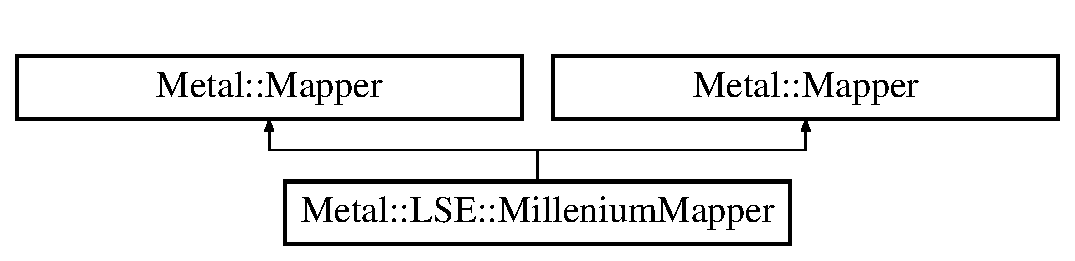
\includegraphics[height=2.000000cm]{classMetal_1_1LSE_1_1MilleniumMapper}
\end{center}
\end{figure}
\subsection*{Public Member Functions}
\begin{DoxyCompactItemize}
\item 
void \hyperlink{classMetal_1_1LSE_1_1MilleniumMapper_a63d9848ac2d8eb7c5e76e50c2d365c79}{benchmark} (std\+::vector$<$ \hyperlink{classMetal_1_1NewOrderSingle}{New\+Order\+Single} $>$ \&)
\end{DoxyCompactItemize}
\subsection*{Static Public Member Functions}
\begin{DoxyCompactItemize}
\item 
static void \hyperlink{classMetal_1_1LSE_1_1MilleniumMapper_a08f65c6357d8b450aff6335bf7dd4de8}{map} (const \hyperlink{classMetal_1_1LSE_1_1NewOrder}{New\+Order} \&, \hyperlink{classMetal_1_1NewOrderSingle}{New\+Order\+Single} \&)
\item 
static void \hyperlink{classMetal_1_1LSE_1_1MilleniumMapper_a83374c3bae042cd654f5f8b64d0584a2}{map} (const \hyperlink{classMetal_1_1NewOrderSingle}{New\+Order\+Single} \&, \hyperlink{classMetal_1_1LSE_1_1NewOrder}{New\+Order} \&)
\item 
static void \hyperlink{classMetal_1_1LSE_1_1MilleniumMapper_a21b4c1861b7c394ecae250baa685ab6d}{map} (const \hyperlink{classMetal_1_1OrderCancelRequest}{Metal\+::\+Order\+Cancel\+Request} \&, \hyperlink{classMetal_1_1LSE_1_1OrderCancelRequest}{Metal\+::\+L\+S\+E\+::\+Order\+Cancel\+Request} \&)
\item 
static void \hyperlink{classMetal_1_1LSE_1_1MilleniumMapper_a430f2f1f1f8dc53821e39ab90f6c78df}{map} (const F\+I\+X\+::\+Side \&, Metal\+::\+L\+S\+E\+::\+Side \&)
\end{DoxyCompactItemize}


\subsection{Member Function Documentation}
\hypertarget{classMetal_1_1LSE_1_1MilleniumMapper_a63d9848ac2d8eb7c5e76e50c2d365c79}{}\index{Metal\+::\+L\+S\+E\+::\+Millenium\+Mapper@{Metal\+::\+L\+S\+E\+::\+Millenium\+Mapper}!benchmark@{benchmark}}
\index{benchmark@{benchmark}!Metal\+::\+L\+S\+E\+::\+Millenium\+Mapper@{Metal\+::\+L\+S\+E\+::\+Millenium\+Mapper}}
\subsubsection[{benchmark}]{\setlength{\rightskip}{0pt plus 5cm}void Metal\+::\+L\+S\+E\+::\+Millenium\+Mapper\+::benchmark (
\begin{DoxyParamCaption}
\item[{std\+::vector$<$ {\bf New\+Order\+Single} $>$ \&}]{all\+Orders}
\end{DoxyParamCaption}
)}\label{classMetal_1_1LSE_1_1MilleniumMapper_a63d9848ac2d8eb7c5e76e50c2d365c79}
This is just a dumb loop that maps all incoming \hyperlink{classMetal_1_1NewOrderSingle}{New\+Order\+Single}. It has no other function than measuring mapping speed \hypertarget{classMetal_1_1LSE_1_1MilleniumMapper_a08f65c6357d8b450aff6335bf7dd4de8}{}\index{Metal\+::\+L\+S\+E\+::\+Millenium\+Mapper@{Metal\+::\+L\+S\+E\+::\+Millenium\+Mapper}!map@{map}}
\index{map@{map}!Metal\+::\+L\+S\+E\+::\+Millenium\+Mapper@{Metal\+::\+L\+S\+E\+::\+Millenium\+Mapper}}
\subsubsection[{map}]{\setlength{\rightskip}{0pt plus 5cm}void Metal\+::\+L\+S\+E\+::\+Millenium\+Mapper\+::map (
\begin{DoxyParamCaption}
\item[{const {\bf New\+Order} \&}]{message, }
\item[{{\bf New\+Order\+Single} \&}]{nos}
\end{DoxyParamCaption}
)\hspace{0.3cm}{\ttfamily [static]}}\label{classMetal_1_1LSE_1_1MilleniumMapper_a08f65c6357d8b450aff6335bf7dd4de8}
Translate L\+S\+E \hyperlink{classMetal_1_1LSE_1_1NewOrder}{New\+Order} into Metal representation \hypertarget{classMetal_1_1LSE_1_1MilleniumMapper_a83374c3bae042cd654f5f8b64d0584a2}{}\index{Metal\+::\+L\+S\+E\+::\+Millenium\+Mapper@{Metal\+::\+L\+S\+E\+::\+Millenium\+Mapper}!map@{map}}
\index{map@{map}!Metal\+::\+L\+S\+E\+::\+Millenium\+Mapper@{Metal\+::\+L\+S\+E\+::\+Millenium\+Mapper}}
\subsubsection[{map}]{\setlength{\rightskip}{0pt plus 5cm}void Metal\+::\+L\+S\+E\+::\+Millenium\+Mapper\+::map (
\begin{DoxyParamCaption}
\item[{const {\bf New\+Order\+Single} \&}]{nos, }
\item[{{\bf New\+Order} \&}]{new\+Order}
\end{DoxyParamCaption}
)\hspace{0.3cm}{\ttfamily [static]}}\label{classMetal_1_1LSE_1_1MilleniumMapper_a83374c3bae042cd654f5f8b64d0584a2}
Me\+T\+A\+L to L\+S\+E for \hyperlink{classMetal_1_1NewOrderSingle}{New\+Order\+Single}

\hyperlink{classMetal_1_1NewOrderSingle}{New\+Order\+Single} Me\+T\+A\+L -\/$>$ L\+S\+E 
\begin{DoxyExceptions}{Exceptions}
{\em F\+I\+X\+::\+Field\+Not\+Found} & \\
\hline
\end{DoxyExceptions}
\hypertarget{classMetal_1_1LSE_1_1MilleniumMapper_a21b4c1861b7c394ecae250baa685ab6d}{}\index{Metal\+::\+L\+S\+E\+::\+Millenium\+Mapper@{Metal\+::\+L\+S\+E\+::\+Millenium\+Mapper}!map@{map}}
\index{map@{map}!Metal\+::\+L\+S\+E\+::\+Millenium\+Mapper@{Metal\+::\+L\+S\+E\+::\+Millenium\+Mapper}}
\subsubsection[{map}]{\setlength{\rightskip}{0pt plus 5cm}void Metal\+::\+L\+S\+E\+::\+Millenium\+Mapper\+::map (
\begin{DoxyParamCaption}
\item[{const {\bf Metal\+::\+Order\+Cancel\+Request} \&}]{ocr\+From, }
\item[{{\bf Metal\+::\+L\+S\+E\+::\+Order\+Cancel\+Request} \&}]{ocr\+To}
\end{DoxyParamCaption}
)\hspace{0.3cm}{\ttfamily [static]}}\label{classMetal_1_1LSE_1_1MilleniumMapper_a21b4c1861b7c394ecae250baa685ab6d}
Me\+T\+A\+L to L\+S\+E for \hyperlink{classMetal_1_1LSE_1_1OrderCancelRequest}{Order\+Cancel\+Request}

Order\+Cancel Request Metal -\/$>$ L\+S\+E \hypertarget{classMetal_1_1LSE_1_1MilleniumMapper_a430f2f1f1f8dc53821e39ab90f6c78df}{}\index{Metal\+::\+L\+S\+E\+::\+Millenium\+Mapper@{Metal\+::\+L\+S\+E\+::\+Millenium\+Mapper}!map@{map}}
\index{map@{map}!Metal\+::\+L\+S\+E\+::\+Millenium\+Mapper@{Metal\+::\+L\+S\+E\+::\+Millenium\+Mapper}}
\subsubsection[{map}]{\setlength{\rightskip}{0pt plus 5cm}void Metal\+::\+L\+S\+E\+::\+Millenium\+Mapper\+::map (
\begin{DoxyParamCaption}
\item[{const F\+I\+X\+::\+Side \&}]{side\+From, }
\item[{Metal\+::\+L\+S\+E\+::\+Side \&}]{side\+To}
\end{DoxyParamCaption}
)\hspace{0.3cm}{\ttfamily [static]}}\label{classMetal_1_1LSE_1_1MilleniumMapper_a430f2f1f1f8dc53821e39ab90f6c78df}
Metal to L\+S\+E for Side

Side Metal -\/$>$ L\+S\+E 

The documentation for this class was generated from the following files\+:\begin{DoxyCompactItemize}
\item 
/home/jc/metal/src/metal/adapters/\+L\+S\+E\+Trading\+Adapter/Millenium\+Mapper.\+h\item 
/home/jc/metal/src/metal/adapters/\+L\+S\+E\+Trading\+Adapter/Millenium\+Mapper.\+cpp\end{DoxyCompactItemize}

\hypertarget{classMetal_1_1MissingImplementationException}{}\section{Metal\+:\+:Missing\+Implementation\+Exception Class Reference}
\label{classMetal_1_1MissingImplementationException}\index{Metal\+::\+Missing\+Implementation\+Exception@{Metal\+::\+Missing\+Implementation\+Exception}}


{\ttfamily \#include $<$Metal\+Exceptions.\+h$>$}

Inheritance diagram for Metal\+:\+:Missing\+Implementation\+Exception\+:\begin{figure}[H]
\begin{center}
\leavevmode
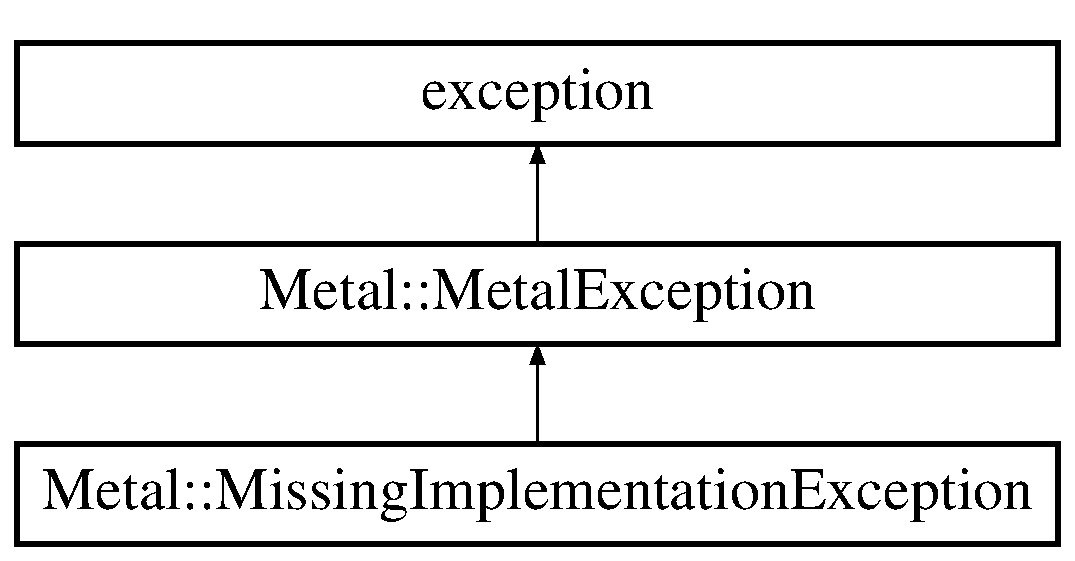
\includegraphics[height=3.000000cm]{classMetal_1_1MissingImplementationException}
\end{center}
\end{figure}
\subsection*{Public Member Functions}
\begin{DoxyCompactItemize}
\item 
\hyperlink{classMetal_1_1MissingImplementationException_a729da91eec41214435d6f946d1524c3d}{Missing\+Implementation\+Exception} (const std\+::string \&message)
\end{DoxyCompactItemize}


\subsection{Constructor \& Destructor Documentation}
\hypertarget{classMetal_1_1MissingImplementationException_a729da91eec41214435d6f946d1524c3d}{}\index{Metal\+::\+Missing\+Implementation\+Exception@{Metal\+::\+Missing\+Implementation\+Exception}!Missing\+Implementation\+Exception@{Missing\+Implementation\+Exception}}
\index{Missing\+Implementation\+Exception@{Missing\+Implementation\+Exception}!Metal\+::\+Missing\+Implementation\+Exception@{Metal\+::\+Missing\+Implementation\+Exception}}
\subsubsection[{Missing\+Implementation\+Exception}]{\setlength{\rightskip}{0pt plus 5cm}Metal\+::\+Missing\+Implementation\+Exception\+::\+Missing\+Implementation\+Exception (
\begin{DoxyParamCaption}
\item[{const std\+::string \&}]{message}
\end{DoxyParamCaption}
)\hspace{0.3cm}{\ttfamily [inline]}}\label{classMetal_1_1MissingImplementationException_a729da91eec41214435d6f946d1524c3d}


The documentation for this class was generated from the following file\+:\begin{DoxyCompactItemize}
\item 
/home/jc/metal/github/include/metal/\hyperlink{MetalExceptions_8h}{Metal\+Exceptions.\+h}\end{DoxyCompactItemize}

\hypertarget{classMetal_1_1QuickFIX_1_1MyApplication}{}\section{Metal\+:\+:Quick\+F\+I\+X\+:\+:My\+Application Class Reference}
\label{classMetal_1_1QuickFIX_1_1MyApplication}\index{Metal\+::\+Quick\+F\+I\+X\+::\+My\+Application@{Metal\+::\+Quick\+F\+I\+X\+::\+My\+Application}}
Inheritance diagram for Metal\+:\+:Quick\+F\+I\+X\+:\+:My\+Application\+:\begin{figure}[H]
\begin{center}
\leavevmode
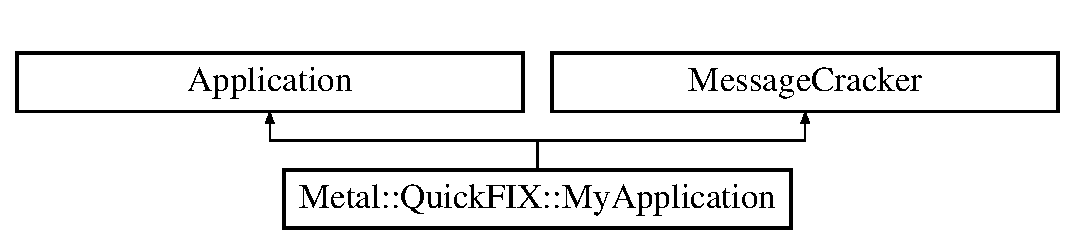
\includegraphics[height=2.000000cm]{classMetal_1_1QuickFIX_1_1MyApplication}
\end{center}
\end{figure}
\subsection*{Public Member Functions}
\begin{DoxyCompactItemize}
\item 
\hyperlink{classMetal_1_1QuickFIX_1_1MyApplication_ac015be7d9bb1677acda6fa464ce0f8ea}{My\+Application} (\hyperlink{classMetal_1_1QuickFIX_1_1QuickFIXAdapter}{Quick\+F\+I\+X\+Adapter} $\ast$pqfa)
\item 
\hyperlink{classMetal_1_1QuickFIX_1_1MyApplication_a1863c717971ba7a4d89dc50ee369abde}{$\sim$\+My\+Application} ()
\item 
void \hyperlink{classMetal_1_1QuickFIX_1_1MyApplication_a3f94210c4e0cbe060de70f7a875195c0}{on\+Create} (const Session\+I\+D \&)
\item 
void \hyperlink{classMetal_1_1QuickFIX_1_1MyApplication_a8dd2c71b6ec276e4f3da25d3b58710b8}{on\+Logon} (const Session\+I\+D \&)
\item 
void \hyperlink{classMetal_1_1QuickFIX_1_1MyApplication_ab5519b36c6fa527fd482bfb6864bad44}{on\+Logout} (const Session\+I\+D \&)
\item 
void \hyperlink{classMetal_1_1QuickFIX_1_1MyApplication_aa884521d47f50ff8c66c4ccd1409e1d6}{to\+Admin} (F\+I\+X\+::\+Message \&, const Session\+I\+D \&)
\item 
void \hyperlink{classMetal_1_1QuickFIX_1_1MyApplication_af32204a063c0a11009652626c86b24d0}{to\+App} (F\+I\+X\+::\+Message \&, const Session\+I\+D \&)  throw ( Do\+Not\+Send )
\item 
void \hyperlink{classMetal_1_1QuickFIX_1_1MyApplication_a4805e0aa8bc992043a2e3a0a4f818221}{from\+Admin} (const F\+I\+X\+::\+Message \&, const Session\+I\+D \&)  throw ( Field\+Not\+Found, Incorrect\+Data\+Format, Incorrect\+Tag\+Value, Reject\+Logon )
\item 
void \hyperlink{classMetal_1_1QuickFIX_1_1MyApplication_aca5ad6dbc249cb4093988887224598a6}{from\+App} (const F\+I\+X\+::\+Message \&message, const Session\+I\+D \&session\+I\+D)  throw ( Field\+Not\+Found, Incorrect\+Data\+Format, Incorrect\+Tag\+Value, Unsupported\+Message\+Type )
\item 
void \hyperlink{classMetal_1_1QuickFIX_1_1MyApplication_a6d513e282a19bbccd0719c39ca5c5dcf}{on\+Message} (const F\+I\+X42\+::\+Execution\+Report \&message, const Session\+I\+D \&)
\item 
void \hyperlink{classMetal_1_1QuickFIX_1_1MyApplication_a0bdc162c886f9aa87b481877d990a084}{on\+Message} (const F\+I\+X44\+::\+Execution\+Report \&message, const Session\+I\+D \&)
\end{DoxyCompactItemize}


\subsection{Constructor \& Destructor Documentation}
\hypertarget{classMetal_1_1QuickFIX_1_1MyApplication_ac015be7d9bb1677acda6fa464ce0f8ea}{}\index{Metal\+::\+Quick\+F\+I\+X\+::\+My\+Application@{Metal\+::\+Quick\+F\+I\+X\+::\+My\+Application}!My\+Application@{My\+Application}}
\index{My\+Application@{My\+Application}!Metal\+::\+Quick\+F\+I\+X\+::\+My\+Application@{Metal\+::\+Quick\+F\+I\+X\+::\+My\+Application}}
\subsubsection[{My\+Application}]{\setlength{\rightskip}{0pt plus 5cm}Metal\+::\+Quick\+F\+I\+X\+::\+My\+Application\+::\+My\+Application (
\begin{DoxyParamCaption}
\item[{{\bf Quick\+F\+I\+X\+Adapter} $\ast$}]{pqfa}
\end{DoxyParamCaption}
)\hspace{0.3cm}{\ttfamily [inline]}}\label{classMetal_1_1QuickFIX_1_1MyApplication_ac015be7d9bb1677acda6fa464ce0f8ea}
\hypertarget{classMetal_1_1QuickFIX_1_1MyApplication_a1863c717971ba7a4d89dc50ee369abde}{}\index{Metal\+::\+Quick\+F\+I\+X\+::\+My\+Application@{Metal\+::\+Quick\+F\+I\+X\+::\+My\+Application}!````~My\+Application@{$\sim$\+My\+Application}}
\index{````~My\+Application@{$\sim$\+My\+Application}!Metal\+::\+Quick\+F\+I\+X\+::\+My\+Application@{Metal\+::\+Quick\+F\+I\+X\+::\+My\+Application}}
\subsubsection[{$\sim$\+My\+Application}]{\setlength{\rightskip}{0pt plus 5cm}Metal\+::\+Quick\+F\+I\+X\+::\+My\+Application\+::$\sim$\+My\+Application (
\begin{DoxyParamCaption}
{}
\end{DoxyParamCaption}
)\hspace{0.3cm}{\ttfamily [inline]}}\label{classMetal_1_1QuickFIX_1_1MyApplication_a1863c717971ba7a4d89dc50ee369abde}


\subsection{Member Function Documentation}
\hypertarget{classMetal_1_1QuickFIX_1_1MyApplication_a4805e0aa8bc992043a2e3a0a4f818221}{}\index{Metal\+::\+Quick\+F\+I\+X\+::\+My\+Application@{Metal\+::\+Quick\+F\+I\+X\+::\+My\+Application}!from\+Admin@{from\+Admin}}
\index{from\+Admin@{from\+Admin}!Metal\+::\+Quick\+F\+I\+X\+::\+My\+Application@{Metal\+::\+Quick\+F\+I\+X\+::\+My\+Application}}
\subsubsection[{from\+Admin}]{\setlength{\rightskip}{0pt plus 5cm}void Metal\+::\+Quick\+F\+I\+X\+::\+My\+Application\+::from\+Admin (
\begin{DoxyParamCaption}
\item[{const F\+I\+X\+::\+Message \&}]{, }
\item[{const Session\+I\+D \&}]{}
\end{DoxyParamCaption}
) throw   Field\+Not\+Found,  Incorrect\+Data\+Format,  Incorrect\+Tag\+Value, Reject\+Logon) \hspace{0.3cm}{\ttfamily [inline]}}\label{classMetal_1_1QuickFIX_1_1MyApplication_a4805e0aa8bc992043a2e3a0a4f818221}
\hypertarget{classMetal_1_1QuickFIX_1_1MyApplication_aca5ad6dbc249cb4093988887224598a6}{}\index{Metal\+::\+Quick\+F\+I\+X\+::\+My\+Application@{Metal\+::\+Quick\+F\+I\+X\+::\+My\+Application}!from\+App@{from\+App}}
\index{from\+App@{from\+App}!Metal\+::\+Quick\+F\+I\+X\+::\+My\+Application@{Metal\+::\+Quick\+F\+I\+X\+::\+My\+Application}}
\subsubsection[{from\+App}]{\setlength{\rightskip}{0pt plus 5cm}void Metal\+::\+Quick\+F\+I\+X\+::\+My\+Application\+::from\+App (
\begin{DoxyParamCaption}
\item[{const F\+I\+X\+::\+Message \&}]{message, }
\item[{const Session\+I\+D \&}]{session\+I\+D}
\end{DoxyParamCaption}
) throw   Field\+Not\+Found,  Incorrect\+Data\+Format,  Incorrect\+Tag\+Value, Unsupported\+Message\+Type) \hspace{0.3cm}{\ttfamily [inline]}}\label{classMetal_1_1QuickFIX_1_1MyApplication_aca5ad6dbc249cb4093988887224598a6}
\hypertarget{classMetal_1_1QuickFIX_1_1MyApplication_a3f94210c4e0cbe060de70f7a875195c0}{}\index{Metal\+::\+Quick\+F\+I\+X\+::\+My\+Application@{Metal\+::\+Quick\+F\+I\+X\+::\+My\+Application}!on\+Create@{on\+Create}}
\index{on\+Create@{on\+Create}!Metal\+::\+Quick\+F\+I\+X\+::\+My\+Application@{Metal\+::\+Quick\+F\+I\+X\+::\+My\+Application}}
\subsubsection[{on\+Create}]{\setlength{\rightskip}{0pt plus 5cm}void Metal\+::\+Quick\+F\+I\+X\+::\+My\+Application\+::on\+Create (
\begin{DoxyParamCaption}
\item[{const Session\+I\+D \&}]{}
\end{DoxyParamCaption}
)\hspace{0.3cm}{\ttfamily [inline]}}\label{classMetal_1_1QuickFIX_1_1MyApplication_a3f94210c4e0cbe060de70f7a875195c0}
\hypertarget{classMetal_1_1QuickFIX_1_1MyApplication_a8dd2c71b6ec276e4f3da25d3b58710b8}{}\index{Metal\+::\+Quick\+F\+I\+X\+::\+My\+Application@{Metal\+::\+Quick\+F\+I\+X\+::\+My\+Application}!on\+Logon@{on\+Logon}}
\index{on\+Logon@{on\+Logon}!Metal\+::\+Quick\+F\+I\+X\+::\+My\+Application@{Metal\+::\+Quick\+F\+I\+X\+::\+My\+Application}}
\subsubsection[{on\+Logon}]{\setlength{\rightskip}{0pt plus 5cm}void Metal\+::\+Quick\+F\+I\+X\+::\+My\+Application\+::on\+Logon (
\begin{DoxyParamCaption}
\item[{const Session\+I\+D \&}]{}
\end{DoxyParamCaption}
)\hspace{0.3cm}{\ttfamily [inline]}}\label{classMetal_1_1QuickFIX_1_1MyApplication_a8dd2c71b6ec276e4f3da25d3b58710b8}
\hypertarget{classMetal_1_1QuickFIX_1_1MyApplication_ab5519b36c6fa527fd482bfb6864bad44}{}\index{Metal\+::\+Quick\+F\+I\+X\+::\+My\+Application@{Metal\+::\+Quick\+F\+I\+X\+::\+My\+Application}!on\+Logout@{on\+Logout}}
\index{on\+Logout@{on\+Logout}!Metal\+::\+Quick\+F\+I\+X\+::\+My\+Application@{Metal\+::\+Quick\+F\+I\+X\+::\+My\+Application}}
\subsubsection[{on\+Logout}]{\setlength{\rightskip}{0pt plus 5cm}void Metal\+::\+Quick\+F\+I\+X\+::\+My\+Application\+::on\+Logout (
\begin{DoxyParamCaption}
\item[{const Session\+I\+D \&}]{}
\end{DoxyParamCaption}
)\hspace{0.3cm}{\ttfamily [inline]}}\label{classMetal_1_1QuickFIX_1_1MyApplication_ab5519b36c6fa527fd482bfb6864bad44}
\hypertarget{classMetal_1_1QuickFIX_1_1MyApplication_a6d513e282a19bbccd0719c39ca5c5dcf}{}\index{Metal\+::\+Quick\+F\+I\+X\+::\+My\+Application@{Metal\+::\+Quick\+F\+I\+X\+::\+My\+Application}!on\+Message@{on\+Message}}
\index{on\+Message@{on\+Message}!Metal\+::\+Quick\+F\+I\+X\+::\+My\+Application@{Metal\+::\+Quick\+F\+I\+X\+::\+My\+Application}}
\subsubsection[{on\+Message}]{\setlength{\rightskip}{0pt plus 5cm}void Metal\+::\+Quick\+F\+I\+X\+::\+My\+Application\+::on\+Message (
\begin{DoxyParamCaption}
\item[{const F\+I\+X42\+::\+Execution\+Report \&}]{message, }
\item[{const Session\+I\+D \&}]{}
\end{DoxyParamCaption}
)\hspace{0.3cm}{\ttfamily [inline]}}\label{classMetal_1_1QuickFIX_1_1MyApplication_a6d513e282a19bbccd0719c39ca5c5dcf}
\hypertarget{classMetal_1_1QuickFIX_1_1MyApplication_a0bdc162c886f9aa87b481877d990a084}{}\index{Metal\+::\+Quick\+F\+I\+X\+::\+My\+Application@{Metal\+::\+Quick\+F\+I\+X\+::\+My\+Application}!on\+Message@{on\+Message}}
\index{on\+Message@{on\+Message}!Metal\+::\+Quick\+F\+I\+X\+::\+My\+Application@{Metal\+::\+Quick\+F\+I\+X\+::\+My\+Application}}
\subsubsection[{on\+Message}]{\setlength{\rightskip}{0pt plus 5cm}void Metal\+::\+Quick\+F\+I\+X\+::\+My\+Application\+::on\+Message (
\begin{DoxyParamCaption}
\item[{const F\+I\+X44\+::\+Execution\+Report \&}]{message, }
\item[{const Session\+I\+D \&}]{}
\end{DoxyParamCaption}
)\hspace{0.3cm}{\ttfamily [inline]}}\label{classMetal_1_1QuickFIX_1_1MyApplication_a0bdc162c886f9aa87b481877d990a084}
\hypertarget{classMetal_1_1QuickFIX_1_1MyApplication_aa884521d47f50ff8c66c4ccd1409e1d6}{}\index{Metal\+::\+Quick\+F\+I\+X\+::\+My\+Application@{Metal\+::\+Quick\+F\+I\+X\+::\+My\+Application}!to\+Admin@{to\+Admin}}
\index{to\+Admin@{to\+Admin}!Metal\+::\+Quick\+F\+I\+X\+::\+My\+Application@{Metal\+::\+Quick\+F\+I\+X\+::\+My\+Application}}
\subsubsection[{to\+Admin}]{\setlength{\rightskip}{0pt plus 5cm}void Metal\+::\+Quick\+F\+I\+X\+::\+My\+Application\+::to\+Admin (
\begin{DoxyParamCaption}
\item[{F\+I\+X\+::\+Message \&}]{, }
\item[{const Session\+I\+D \&}]{}
\end{DoxyParamCaption}
)\hspace{0.3cm}{\ttfamily [inline]}}\label{classMetal_1_1QuickFIX_1_1MyApplication_aa884521d47f50ff8c66c4ccd1409e1d6}
\hypertarget{classMetal_1_1QuickFIX_1_1MyApplication_af32204a063c0a11009652626c86b24d0}{}\index{Metal\+::\+Quick\+F\+I\+X\+::\+My\+Application@{Metal\+::\+Quick\+F\+I\+X\+::\+My\+Application}!to\+App@{to\+App}}
\index{to\+App@{to\+App}!Metal\+::\+Quick\+F\+I\+X\+::\+My\+Application@{Metal\+::\+Quick\+F\+I\+X\+::\+My\+Application}}
\subsubsection[{to\+App}]{\setlength{\rightskip}{0pt plus 5cm}void Metal\+::\+Quick\+F\+I\+X\+::\+My\+Application\+::to\+App (
\begin{DoxyParamCaption}
\item[{F\+I\+X\+::\+Message \&}]{, }
\item[{const Session\+I\+D \&}]{}
\end{DoxyParamCaption}
) throw  Do\+Not\+Send) \hspace{0.3cm}{\ttfamily [inline]}}\label{classMetal_1_1QuickFIX_1_1MyApplication_af32204a063c0a11009652626c86b24d0}


The documentation for this class was generated from the following file\+:\begin{DoxyCompactItemize}
\item 
/home/jc/metal/github/src/adapters/\+Quick\+F\+I\+X\+Adapter/\hyperlink{QuickFIXAdapter_8cpp}{Quick\+F\+I\+X\+Adapter.\+cpp}\end{DoxyCompactItemize}

\hypertarget{unionNativeValue}{}\section{Native\+Value Union Reference}
\label{unionNativeValue}\index{Native\+Value@{Native\+Value}}


{\ttfamily \#include $<$Native\+Values.\+h$>$}

\subsection*{Public Attributes}
\begin{DoxyCompactItemize}
\item 
int8\+\_\+t \hyperlink{unionNativeValue_afa6c11e7310444fc54b52672f29b0851}{i8}
\item 
int16\+\_\+t \hyperlink{unionNativeValue_acf12bb9ab3bad9b103af275e5dbefe9d}{i16}
\item 
int32\+\_\+t \hyperlink{unionNativeValue_a4cbe7f42324173b29515dee236baf2c2}{i32}
\item 
int64\+\_\+t \hyperlink{unionNativeValue_ac0d957c8cb327ccf915b6de922fc8444}{i64}
\item 
uint8\+\_\+t \hyperlink{unionNativeValue_a828b63673532c2c53493f96453b3826f}{u8}
\item 
uint16\+\_\+t \hyperlink{unionNativeValue_ac8680bbb0804d550c485c942181490fe}{u16}
\item 
uint32\+\_\+t \hyperlink{unionNativeValue_adbe240086e05df57038bafbbe316a323}{u32}
\item 
uint64\+\_\+t \hyperlink{unionNativeValue_a4c6ef6c5f3ffdd7b7a662304bef89d4c}{u64}
\item 
char \hyperlink{unionNativeValue_adee38de50b0a6c4d36db7fbab7f8e526}{str} \mbox{[}128\mbox{]}
\end{DoxyCompactItemize}


\subsection{Member Data Documentation}
\hypertarget{unionNativeValue_acf12bb9ab3bad9b103af275e5dbefe9d}{}\index{Native\+Value@{Native\+Value}!i16@{i16}}
\index{i16@{i16}!Native\+Value@{Native\+Value}}
\subsubsection[{i16}]{\setlength{\rightskip}{0pt plus 5cm}int16\+\_\+t Native\+Value\+::i16}\label{unionNativeValue_acf12bb9ab3bad9b103af275e5dbefe9d}
\hypertarget{unionNativeValue_a4cbe7f42324173b29515dee236baf2c2}{}\index{Native\+Value@{Native\+Value}!i32@{i32}}
\index{i32@{i32}!Native\+Value@{Native\+Value}}
\subsubsection[{i32}]{\setlength{\rightskip}{0pt plus 5cm}int32\+\_\+t Native\+Value\+::i32}\label{unionNativeValue_a4cbe7f42324173b29515dee236baf2c2}
\hypertarget{unionNativeValue_ac0d957c8cb327ccf915b6de922fc8444}{}\index{Native\+Value@{Native\+Value}!i64@{i64}}
\index{i64@{i64}!Native\+Value@{Native\+Value}}
\subsubsection[{i64}]{\setlength{\rightskip}{0pt plus 5cm}int64\+\_\+t Native\+Value\+::i64}\label{unionNativeValue_ac0d957c8cb327ccf915b6de922fc8444}
\hypertarget{unionNativeValue_afa6c11e7310444fc54b52672f29b0851}{}\index{Native\+Value@{Native\+Value}!i8@{i8}}
\index{i8@{i8}!Native\+Value@{Native\+Value}}
\subsubsection[{i8}]{\setlength{\rightskip}{0pt plus 5cm}int8\+\_\+t Native\+Value\+::i8}\label{unionNativeValue_afa6c11e7310444fc54b52672f29b0851}
\hypertarget{unionNativeValue_adee38de50b0a6c4d36db7fbab7f8e526}{}\index{Native\+Value@{Native\+Value}!str@{str}}
\index{str@{str}!Native\+Value@{Native\+Value}}
\subsubsection[{str}]{\setlength{\rightskip}{0pt plus 5cm}char Native\+Value\+::str\mbox{[}128\mbox{]}}\label{unionNativeValue_adee38de50b0a6c4d36db7fbab7f8e526}
\hypertarget{unionNativeValue_ac8680bbb0804d550c485c942181490fe}{}\index{Native\+Value@{Native\+Value}!u16@{u16}}
\index{u16@{u16}!Native\+Value@{Native\+Value}}
\subsubsection[{u16}]{\setlength{\rightskip}{0pt plus 5cm}uint16\+\_\+t Native\+Value\+::u16}\label{unionNativeValue_ac8680bbb0804d550c485c942181490fe}
\hypertarget{unionNativeValue_adbe240086e05df57038bafbbe316a323}{}\index{Native\+Value@{Native\+Value}!u32@{u32}}
\index{u32@{u32}!Native\+Value@{Native\+Value}}
\subsubsection[{u32}]{\setlength{\rightskip}{0pt plus 5cm}uint32\+\_\+t Native\+Value\+::u32}\label{unionNativeValue_adbe240086e05df57038bafbbe316a323}
\hypertarget{unionNativeValue_a4c6ef6c5f3ffdd7b7a662304bef89d4c}{}\index{Native\+Value@{Native\+Value}!u64@{u64}}
\index{u64@{u64}!Native\+Value@{Native\+Value}}
\subsubsection[{u64}]{\setlength{\rightskip}{0pt plus 5cm}uint64\+\_\+t Native\+Value\+::u64}\label{unionNativeValue_a4c6ef6c5f3ffdd7b7a662304bef89d4c}
\hypertarget{unionNativeValue_a828b63673532c2c53493f96453b3826f}{}\index{Native\+Value@{Native\+Value}!u8@{u8}}
\index{u8@{u8}!Native\+Value@{Native\+Value}}
\subsubsection[{u8}]{\setlength{\rightskip}{0pt plus 5cm}uint8\+\_\+t Native\+Value\+::u8}\label{unionNativeValue_a828b63673532c2c53493f96453b3826f}


The documentation for this union was generated from the following file\+:\begin{DoxyCompactItemize}
\item 
/home/jc/metal/github/src/bootstrapper/\hyperlink{NativeValues_8h}{Native\+Values.\+h}\end{DoxyCompactItemize}

\hypertarget{classMetal_1_1LSE_1_1NewOrder}{}\section{Metal\+:\+:L\+S\+E\+:\+:New\+Order Class Reference}
\label{classMetal_1_1LSE_1_1NewOrder}\index{Metal\+::\+L\+S\+E\+::\+New\+Order@{Metal\+::\+L\+S\+E\+::\+New\+Order}}


{\ttfamily \#include $<$New\+Order.\+h$>$}

\subsection*{Public Member Functions}
\begin{DoxyCompactItemize}
\item 
\hyperlink{classMetal_1_1LSE_1_1NewOrder_aeaedaf6e5ebd46fbb1448b95c2791dcd}{New\+Order} ()
\item 
virtual \hyperlink{classMetal_1_1LSE_1_1NewOrder_acf2c36880aedda0edef97616a8d002fd}{$\sim$\+New\+Order} ()
\end{DoxyCompactItemize}
\subsection*{Public Attributes}
\begin{DoxyCompactItemize}
\item 
std\+::string \hyperlink{classMetal_1_1LSE_1_1NewOrder_a53ce2b8f89f168c58fa2a8f97ce79c93}{client\+Order\+I\+D}
\item 
std\+::string \hyperlink{classMetal_1_1LSE_1_1NewOrder_aff72605e8542180dad099904873bda84}{trader\+I\+D}
\item 
std\+::string \hyperlink{classMetal_1_1LSE_1_1NewOrder_a80ad2239737f52a61a27eb4f6193bdba}{account}
\item 
\hyperlink{namespaceMetal_1_1LSE_ae1f2b67d6be84798adfd29525ee0a697}{Clearing\+Acount} \hyperlink{classMetal_1_1LSE_1_1NewOrder_a65522450bdc6e5ac29e739738bbba34e}{clearing\+Account}
\item 
\hyperlink{namespaceMetal_1_1LSE_a5280aa41aaa4433df351e733a23ecd14}{Instrument\+I\+D} \hyperlink{classMetal_1_1LSE_1_1NewOrder_aeffc76c3cb37c6bd7f6e2a9c5fa4d441}{instrument\+I\+D}
\item 
\hyperlink{namespaceMetal_1_1LSE_aff01f13ff9de4cacdd0436f6956df4fb}{Order\+Type} \hyperlink{classMetal_1_1LSE_1_1NewOrder_aca679f638141bbae5505ed8bb6961378}{order\+Type}
\item 
\hyperlink{namespaceMetal_1_1LSE_a59a4a742606e572af3f14a34a7503ee9}{Time\+In\+Force} \hyperlink{classMetal_1_1LSE_1_1NewOrder_ab0da192ab665eeffa7797f901d2f94fc}{time\+In\+Force}
\item 
\hyperlink{namespaceMetal_1_1LSE_a62b04587ecad5f88a7fbd626194b3c28}{Expire\+Date\+Time} \hyperlink{classMetal_1_1LSE_1_1NewOrder_a75f27f7515b6214b615681e5fc5074c3}{expire\+Date\+Time}
\item 
\hyperlink{namespaceMetal_1_1LSE_af5236b7a999484d8cd5b579b7d7c133b}{Side} \hyperlink{classMetal_1_1LSE_1_1NewOrder_ac13fa3b75b0b41ee60fb6fcf3b57fb31}{side}
\item 
\hyperlink{namespaceMetal_1_1LSE_a86342859fb8034a9649f6d789e97d9da}{Quantity} \hyperlink{classMetal_1_1LSE_1_1NewOrder_a79d35c9c9c65c2acded727062c1b70bd}{order\+Qty}
\item 
\hyperlink{namespaceMetal_1_1LSE_a86342859fb8034a9649f6d789e97d9da}{Quantity} \hyperlink{classMetal_1_1LSE_1_1NewOrder_a7cae6ab56cd3c9a8f973005f0aaaf27e}{display\+Qty}
\item 
\hyperlink{namespaceMetal_1_1LSE_a4a629b5e2aed21d653db0debf8b63af4}{Price} \hyperlink{classMetal_1_1LSE_1_1NewOrder_acff28c03d42db0449f23f480be72c3a9}{limit\+Price}
\item 
\hyperlink{namespaceMetal_1_1LSE_aff7400475e278748e213fefa47bb9b99}{Capacity} \hyperlink{classMetal_1_1LSE_1_1NewOrder_aeace92cd76c0bb8539f82fdfff170115}{capacity}
\item 
\hyperlink{namespaceMetal_1_1LSE_a28e46ba33ca9d641a9ea0c63a2e35141}{Auto\+Cancel} \hyperlink{classMetal_1_1LSE_1_1NewOrder_aacc7198bc8dee4a9bf98bd8bc13dc85b}{auto\+Cancel}
\item 
\hyperlink{namespaceMetal_1_1LSE_afd57250a16de7395f5ad2bc63c7b8e5e}{Order\+Sub\+Type} \hyperlink{classMetal_1_1LSE_1_1NewOrder_a11797541566225395362ff7f9c0e3557}{order\+Sub\+Type}
\item 
\hyperlink{namespaceMetal_1_1LSE_a0c110efde74bd7f4315615c477dac047}{Anonymity} \hyperlink{classMetal_1_1LSE_1_1NewOrder_ab9c132be0c599c5d113d20603bb6f19d}{anonymity}
\item 
\hyperlink{namespaceMetal_1_1LSE_a4a629b5e2aed21d653db0debf8b63af4}{Price} \hyperlink{classMetal_1_1LSE_1_1NewOrder_abf0f20401650effe0dba393616128d0b}{stopped\+Price}
\item 
\hyperlink{namespaceMetal_1_1LSE_afb7bdec752b9048b6d725e2421586a64}{Passive\+Only\+Order} \hyperlink{classMetal_1_1LSE_1_1NewOrder_a4debc1666c97f2c3127ed05fe9373856}{passive\+Only\+Order}
\end{DoxyCompactItemize}
\subsection*{Static Public Attributes}
\begin{DoxyCompactItemize}
\item 
static const int \hyperlink{classMetal_1_1LSE_1_1NewOrder_a1b9c8980a62d9902914b215a139740ba}{S\+I\+Z\+E} = 97
\end{DoxyCompactItemize}


\subsection{Constructor \& Destructor Documentation}
\hypertarget{classMetal_1_1LSE_1_1NewOrder_aeaedaf6e5ebd46fbb1448b95c2791dcd}{}\index{Metal\+::\+L\+S\+E\+::\+New\+Order@{Metal\+::\+L\+S\+E\+::\+New\+Order}!New\+Order@{New\+Order}}
\index{New\+Order@{New\+Order}!Metal\+::\+L\+S\+E\+::\+New\+Order@{Metal\+::\+L\+S\+E\+::\+New\+Order}}
\subsubsection[{New\+Order}]{\setlength{\rightskip}{0pt plus 5cm}Metal\+::\+L\+S\+E\+::\+New\+Order\+::\+New\+Order (
\begin{DoxyParamCaption}
{}
\end{DoxyParamCaption}
)}\label{classMetal_1_1LSE_1_1NewOrder_aeaedaf6e5ebd46fbb1448b95c2791dcd}
\hypertarget{classMetal_1_1LSE_1_1NewOrder_acf2c36880aedda0edef97616a8d002fd}{}\index{Metal\+::\+L\+S\+E\+::\+New\+Order@{Metal\+::\+L\+S\+E\+::\+New\+Order}!````~New\+Order@{$\sim$\+New\+Order}}
\index{````~New\+Order@{$\sim$\+New\+Order}!Metal\+::\+L\+S\+E\+::\+New\+Order@{Metal\+::\+L\+S\+E\+::\+New\+Order}}
\subsubsection[{$\sim$\+New\+Order}]{\setlength{\rightskip}{0pt plus 5cm}Metal\+::\+L\+S\+E\+::\+New\+Order\+::$\sim$\+New\+Order (
\begin{DoxyParamCaption}
{}
\end{DoxyParamCaption}
)\hspace{0.3cm}{\ttfamily [virtual]}}\label{classMetal_1_1LSE_1_1NewOrder_acf2c36880aedda0edef97616a8d002fd}


\subsection{Member Data Documentation}
\hypertarget{classMetal_1_1LSE_1_1NewOrder_a80ad2239737f52a61a27eb4f6193bdba}{}\index{Metal\+::\+L\+S\+E\+::\+New\+Order@{Metal\+::\+L\+S\+E\+::\+New\+Order}!account@{account}}
\index{account@{account}!Metal\+::\+L\+S\+E\+::\+New\+Order@{Metal\+::\+L\+S\+E\+::\+New\+Order}}
\subsubsection[{account}]{\setlength{\rightskip}{0pt plus 5cm}std\+::string Metal\+::\+L\+S\+E\+::\+New\+Order\+::account}\label{classMetal_1_1LSE_1_1NewOrder_a80ad2239737f52a61a27eb4f6193bdba}
\hypertarget{classMetal_1_1LSE_1_1NewOrder_ab9c132be0c599c5d113d20603bb6f19d}{}\index{Metal\+::\+L\+S\+E\+::\+New\+Order@{Metal\+::\+L\+S\+E\+::\+New\+Order}!anonymity@{anonymity}}
\index{anonymity@{anonymity}!Metal\+::\+L\+S\+E\+::\+New\+Order@{Metal\+::\+L\+S\+E\+::\+New\+Order}}
\subsubsection[{anonymity}]{\setlength{\rightskip}{0pt plus 5cm}{\bf Anonymity} Metal\+::\+L\+S\+E\+::\+New\+Order\+::anonymity}\label{classMetal_1_1LSE_1_1NewOrder_ab9c132be0c599c5d113d20603bb6f19d}
\hypertarget{classMetal_1_1LSE_1_1NewOrder_aacc7198bc8dee4a9bf98bd8bc13dc85b}{}\index{Metal\+::\+L\+S\+E\+::\+New\+Order@{Metal\+::\+L\+S\+E\+::\+New\+Order}!auto\+Cancel@{auto\+Cancel}}
\index{auto\+Cancel@{auto\+Cancel}!Metal\+::\+L\+S\+E\+::\+New\+Order@{Metal\+::\+L\+S\+E\+::\+New\+Order}}
\subsubsection[{auto\+Cancel}]{\setlength{\rightskip}{0pt plus 5cm}{\bf Auto\+Cancel} Metal\+::\+L\+S\+E\+::\+New\+Order\+::auto\+Cancel}\label{classMetal_1_1LSE_1_1NewOrder_aacc7198bc8dee4a9bf98bd8bc13dc85b}
\hypertarget{classMetal_1_1LSE_1_1NewOrder_aeace92cd76c0bb8539f82fdfff170115}{}\index{Metal\+::\+L\+S\+E\+::\+New\+Order@{Metal\+::\+L\+S\+E\+::\+New\+Order}!capacity@{capacity}}
\index{capacity@{capacity}!Metal\+::\+L\+S\+E\+::\+New\+Order@{Metal\+::\+L\+S\+E\+::\+New\+Order}}
\subsubsection[{capacity}]{\setlength{\rightskip}{0pt plus 5cm}{\bf Capacity} Metal\+::\+L\+S\+E\+::\+New\+Order\+::capacity}\label{classMetal_1_1LSE_1_1NewOrder_aeace92cd76c0bb8539f82fdfff170115}
\hypertarget{classMetal_1_1LSE_1_1NewOrder_a65522450bdc6e5ac29e739738bbba34e}{}\index{Metal\+::\+L\+S\+E\+::\+New\+Order@{Metal\+::\+L\+S\+E\+::\+New\+Order}!clearing\+Account@{clearing\+Account}}
\index{clearing\+Account@{clearing\+Account}!Metal\+::\+L\+S\+E\+::\+New\+Order@{Metal\+::\+L\+S\+E\+::\+New\+Order}}
\subsubsection[{clearing\+Account}]{\setlength{\rightskip}{0pt plus 5cm}{\bf Clearing\+Acount} Metal\+::\+L\+S\+E\+::\+New\+Order\+::clearing\+Account}\label{classMetal_1_1LSE_1_1NewOrder_a65522450bdc6e5ac29e739738bbba34e}
\hypertarget{classMetal_1_1LSE_1_1NewOrder_a53ce2b8f89f168c58fa2a8f97ce79c93}{}\index{Metal\+::\+L\+S\+E\+::\+New\+Order@{Metal\+::\+L\+S\+E\+::\+New\+Order}!client\+Order\+I\+D@{client\+Order\+I\+D}}
\index{client\+Order\+I\+D@{client\+Order\+I\+D}!Metal\+::\+L\+S\+E\+::\+New\+Order@{Metal\+::\+L\+S\+E\+::\+New\+Order}}
\subsubsection[{client\+Order\+I\+D}]{\setlength{\rightskip}{0pt plus 5cm}std\+::string Metal\+::\+L\+S\+E\+::\+New\+Order\+::client\+Order\+I\+D}\label{classMetal_1_1LSE_1_1NewOrder_a53ce2b8f89f168c58fa2a8f97ce79c93}
\hypertarget{classMetal_1_1LSE_1_1NewOrder_a7cae6ab56cd3c9a8f973005f0aaaf27e}{}\index{Metal\+::\+L\+S\+E\+::\+New\+Order@{Metal\+::\+L\+S\+E\+::\+New\+Order}!display\+Qty@{display\+Qty}}
\index{display\+Qty@{display\+Qty}!Metal\+::\+L\+S\+E\+::\+New\+Order@{Metal\+::\+L\+S\+E\+::\+New\+Order}}
\subsubsection[{display\+Qty}]{\setlength{\rightskip}{0pt plus 5cm}{\bf Quantity} Metal\+::\+L\+S\+E\+::\+New\+Order\+::display\+Qty}\label{classMetal_1_1LSE_1_1NewOrder_a7cae6ab56cd3c9a8f973005f0aaaf27e}
\hypertarget{classMetal_1_1LSE_1_1NewOrder_a75f27f7515b6214b615681e5fc5074c3}{}\index{Metal\+::\+L\+S\+E\+::\+New\+Order@{Metal\+::\+L\+S\+E\+::\+New\+Order}!expire\+Date\+Time@{expire\+Date\+Time}}
\index{expire\+Date\+Time@{expire\+Date\+Time}!Metal\+::\+L\+S\+E\+::\+New\+Order@{Metal\+::\+L\+S\+E\+::\+New\+Order}}
\subsubsection[{expire\+Date\+Time}]{\setlength{\rightskip}{0pt plus 5cm}{\bf Expire\+Date\+Time} Metal\+::\+L\+S\+E\+::\+New\+Order\+::expire\+Date\+Time}\label{classMetal_1_1LSE_1_1NewOrder_a75f27f7515b6214b615681e5fc5074c3}
\hypertarget{classMetal_1_1LSE_1_1NewOrder_aeffc76c3cb37c6bd7f6e2a9c5fa4d441}{}\index{Metal\+::\+L\+S\+E\+::\+New\+Order@{Metal\+::\+L\+S\+E\+::\+New\+Order}!instrument\+I\+D@{instrument\+I\+D}}
\index{instrument\+I\+D@{instrument\+I\+D}!Metal\+::\+L\+S\+E\+::\+New\+Order@{Metal\+::\+L\+S\+E\+::\+New\+Order}}
\subsubsection[{instrument\+I\+D}]{\setlength{\rightskip}{0pt plus 5cm}{\bf Instrument\+I\+D} Metal\+::\+L\+S\+E\+::\+New\+Order\+::instrument\+I\+D}\label{classMetal_1_1LSE_1_1NewOrder_aeffc76c3cb37c6bd7f6e2a9c5fa4d441}
\hypertarget{classMetal_1_1LSE_1_1NewOrder_acff28c03d42db0449f23f480be72c3a9}{}\index{Metal\+::\+L\+S\+E\+::\+New\+Order@{Metal\+::\+L\+S\+E\+::\+New\+Order}!limit\+Price@{limit\+Price}}
\index{limit\+Price@{limit\+Price}!Metal\+::\+L\+S\+E\+::\+New\+Order@{Metal\+::\+L\+S\+E\+::\+New\+Order}}
\subsubsection[{limit\+Price}]{\setlength{\rightskip}{0pt plus 5cm}{\bf Price} Metal\+::\+L\+S\+E\+::\+New\+Order\+::limit\+Price}\label{classMetal_1_1LSE_1_1NewOrder_acff28c03d42db0449f23f480be72c3a9}
Price is stored with 8 implied decimal places \hypertarget{classMetal_1_1LSE_1_1NewOrder_a79d35c9c9c65c2acded727062c1b70bd}{}\index{Metal\+::\+L\+S\+E\+::\+New\+Order@{Metal\+::\+L\+S\+E\+::\+New\+Order}!order\+Qty@{order\+Qty}}
\index{order\+Qty@{order\+Qty}!Metal\+::\+L\+S\+E\+::\+New\+Order@{Metal\+::\+L\+S\+E\+::\+New\+Order}}
\subsubsection[{order\+Qty}]{\setlength{\rightskip}{0pt plus 5cm}{\bf Quantity} Metal\+::\+L\+S\+E\+::\+New\+Order\+::order\+Qty}\label{classMetal_1_1LSE_1_1NewOrder_a79d35c9c9c65c2acded727062c1b70bd}
\hypertarget{classMetal_1_1LSE_1_1NewOrder_a11797541566225395362ff7f9c0e3557}{}\index{Metal\+::\+L\+S\+E\+::\+New\+Order@{Metal\+::\+L\+S\+E\+::\+New\+Order}!order\+Sub\+Type@{order\+Sub\+Type}}
\index{order\+Sub\+Type@{order\+Sub\+Type}!Metal\+::\+L\+S\+E\+::\+New\+Order@{Metal\+::\+L\+S\+E\+::\+New\+Order}}
\subsubsection[{order\+Sub\+Type}]{\setlength{\rightskip}{0pt plus 5cm}{\bf Order\+Sub\+Type} Metal\+::\+L\+S\+E\+::\+New\+Order\+::order\+Sub\+Type}\label{classMetal_1_1LSE_1_1NewOrder_a11797541566225395362ff7f9c0e3557}
\hypertarget{classMetal_1_1LSE_1_1NewOrder_aca679f638141bbae5505ed8bb6961378}{}\index{Metal\+::\+L\+S\+E\+::\+New\+Order@{Metal\+::\+L\+S\+E\+::\+New\+Order}!order\+Type@{order\+Type}}
\index{order\+Type@{order\+Type}!Metal\+::\+L\+S\+E\+::\+New\+Order@{Metal\+::\+L\+S\+E\+::\+New\+Order}}
\subsubsection[{order\+Type}]{\setlength{\rightskip}{0pt plus 5cm}{\bf Order\+Type} Metal\+::\+L\+S\+E\+::\+New\+Order\+::order\+Type}\label{classMetal_1_1LSE_1_1NewOrder_aca679f638141bbae5505ed8bb6961378}
\hypertarget{classMetal_1_1LSE_1_1NewOrder_a4debc1666c97f2c3127ed05fe9373856}{}\index{Metal\+::\+L\+S\+E\+::\+New\+Order@{Metal\+::\+L\+S\+E\+::\+New\+Order}!passive\+Only\+Order@{passive\+Only\+Order}}
\index{passive\+Only\+Order@{passive\+Only\+Order}!Metal\+::\+L\+S\+E\+::\+New\+Order@{Metal\+::\+L\+S\+E\+::\+New\+Order}}
\subsubsection[{passive\+Only\+Order}]{\setlength{\rightskip}{0pt plus 5cm}{\bf Passive\+Only\+Order} Metal\+::\+L\+S\+E\+::\+New\+Order\+::passive\+Only\+Order}\label{classMetal_1_1LSE_1_1NewOrder_a4debc1666c97f2c3127ed05fe9373856}
\hypertarget{classMetal_1_1LSE_1_1NewOrder_ac13fa3b75b0b41ee60fb6fcf3b57fb31}{}\index{Metal\+::\+L\+S\+E\+::\+New\+Order@{Metal\+::\+L\+S\+E\+::\+New\+Order}!side@{side}}
\index{side@{side}!Metal\+::\+L\+S\+E\+::\+New\+Order@{Metal\+::\+L\+S\+E\+::\+New\+Order}}
\subsubsection[{side}]{\setlength{\rightskip}{0pt plus 5cm}{\bf Side} Metal\+::\+L\+S\+E\+::\+New\+Order\+::side}\label{classMetal_1_1LSE_1_1NewOrder_ac13fa3b75b0b41ee60fb6fcf3b57fb31}
\hypertarget{classMetal_1_1LSE_1_1NewOrder_a1b9c8980a62d9902914b215a139740ba}{}\index{Metal\+::\+L\+S\+E\+::\+New\+Order@{Metal\+::\+L\+S\+E\+::\+New\+Order}!S\+I\+Z\+E@{S\+I\+Z\+E}}
\index{S\+I\+Z\+E@{S\+I\+Z\+E}!Metal\+::\+L\+S\+E\+::\+New\+Order@{Metal\+::\+L\+S\+E\+::\+New\+Order}}
\subsubsection[{S\+I\+Z\+E}]{\setlength{\rightskip}{0pt plus 5cm}const int Metal\+::\+L\+S\+E\+::\+New\+Order\+::\+S\+I\+Z\+E = 97\hspace{0.3cm}{\ttfamily [static]}}\label{classMetal_1_1LSE_1_1NewOrder_a1b9c8980a62d9902914b215a139740ba}
\hypertarget{classMetal_1_1LSE_1_1NewOrder_abf0f20401650effe0dba393616128d0b}{}\index{Metal\+::\+L\+S\+E\+::\+New\+Order@{Metal\+::\+L\+S\+E\+::\+New\+Order}!stopped\+Price@{stopped\+Price}}
\index{stopped\+Price@{stopped\+Price}!Metal\+::\+L\+S\+E\+::\+New\+Order@{Metal\+::\+L\+S\+E\+::\+New\+Order}}
\subsubsection[{stopped\+Price}]{\setlength{\rightskip}{0pt plus 5cm}{\bf Price} Metal\+::\+L\+S\+E\+::\+New\+Order\+::stopped\+Price}\label{classMetal_1_1LSE_1_1NewOrder_abf0f20401650effe0dba393616128d0b}
\hypertarget{classMetal_1_1LSE_1_1NewOrder_ab0da192ab665eeffa7797f901d2f94fc}{}\index{Metal\+::\+L\+S\+E\+::\+New\+Order@{Metal\+::\+L\+S\+E\+::\+New\+Order}!time\+In\+Force@{time\+In\+Force}}
\index{time\+In\+Force@{time\+In\+Force}!Metal\+::\+L\+S\+E\+::\+New\+Order@{Metal\+::\+L\+S\+E\+::\+New\+Order}}
\subsubsection[{time\+In\+Force}]{\setlength{\rightskip}{0pt plus 5cm}{\bf Time\+In\+Force} Metal\+::\+L\+S\+E\+::\+New\+Order\+::time\+In\+Force}\label{classMetal_1_1LSE_1_1NewOrder_ab0da192ab665eeffa7797f901d2f94fc}
\hypertarget{classMetal_1_1LSE_1_1NewOrder_aff72605e8542180dad099904873bda84}{}\index{Metal\+::\+L\+S\+E\+::\+New\+Order@{Metal\+::\+L\+S\+E\+::\+New\+Order}!trader\+I\+D@{trader\+I\+D}}
\index{trader\+I\+D@{trader\+I\+D}!Metal\+::\+L\+S\+E\+::\+New\+Order@{Metal\+::\+L\+S\+E\+::\+New\+Order}}
\subsubsection[{trader\+I\+D}]{\setlength{\rightskip}{0pt plus 5cm}std\+::string Metal\+::\+L\+S\+E\+::\+New\+Order\+::trader\+I\+D}\label{classMetal_1_1LSE_1_1NewOrder_aff72605e8542180dad099904873bda84}


The documentation for this class was generated from the following files\+:\begin{DoxyCompactItemize}
\item 
/home/jc/metal/github/src/adapters/\+L\+S\+E\+Trading\+Adapter/\hyperlink{NewOrder_8h}{New\+Order.\+h}\item 
/home/jc/metal/github/src/adapters/\+L\+S\+E\+Trading\+Adapter/\hyperlink{NewOrder_8cpp}{New\+Order.\+cpp}\end{DoxyCompactItemize}

\hypertarget{classMetal_1_1NewOrderSingle}{}\section{Metal\+:\+:New\+Order\+Single Class Reference}
\label{classMetal_1_1NewOrderSingle}\index{Metal\+::\+New\+Order\+Single@{Metal\+::\+New\+Order\+Single}}
Inheritance diagram for Metal\+:\+:New\+Order\+Single\+:\begin{figure}[H]
\begin{center}
\leavevmode
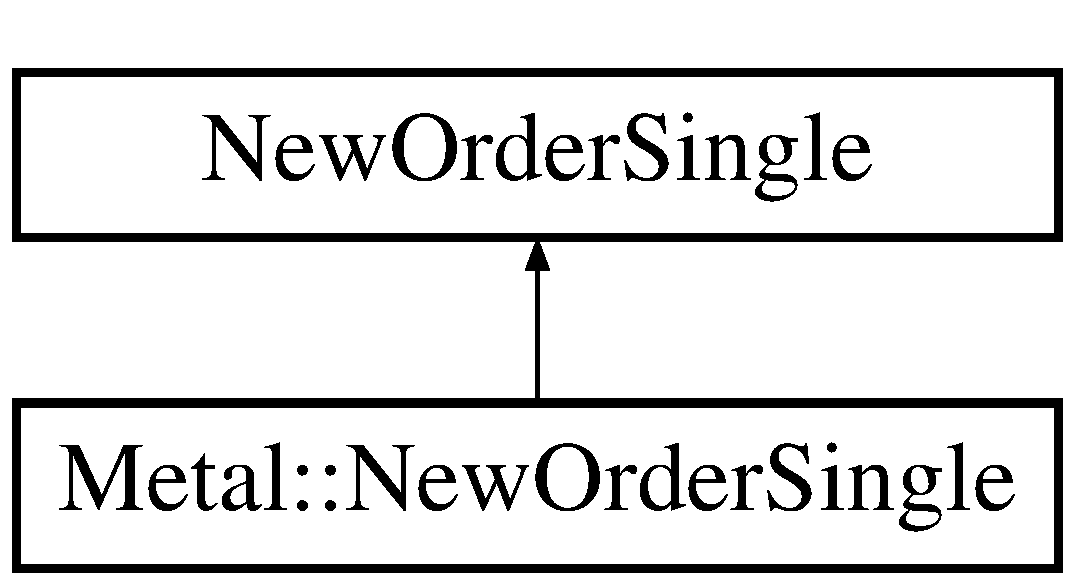
\includegraphics[height=2.000000cm]{classMetal_1_1NewOrderSingle}
\end{center}
\end{figure}


The documentation for this class was generated from the following file\+:\begin{DoxyCompactItemize}
\item 
/home/jc/metal/src/metal/metal.\+h\end{DoxyCompactItemize}

\hypertarget{classMetal_1_1LSE_1_1NormalizedMillenium}{}\section{Metal\+:\+:L\+S\+E\+:\+:Normalized\+Millenium Class Reference}
\label{classMetal_1_1LSE_1_1NormalizedMillenium}\index{Metal\+::\+L\+S\+E\+::\+Normalized\+Millenium@{Metal\+::\+L\+S\+E\+::\+Normalized\+Millenium}}


{\ttfamily \#include $<$Normalized\+Millenium.\+h$>$}

Inheritance diagram for Metal\+:\+:L\+S\+E\+:\+:Normalized\+Millenium\+:\begin{figure}[H]
\begin{center}
\leavevmode
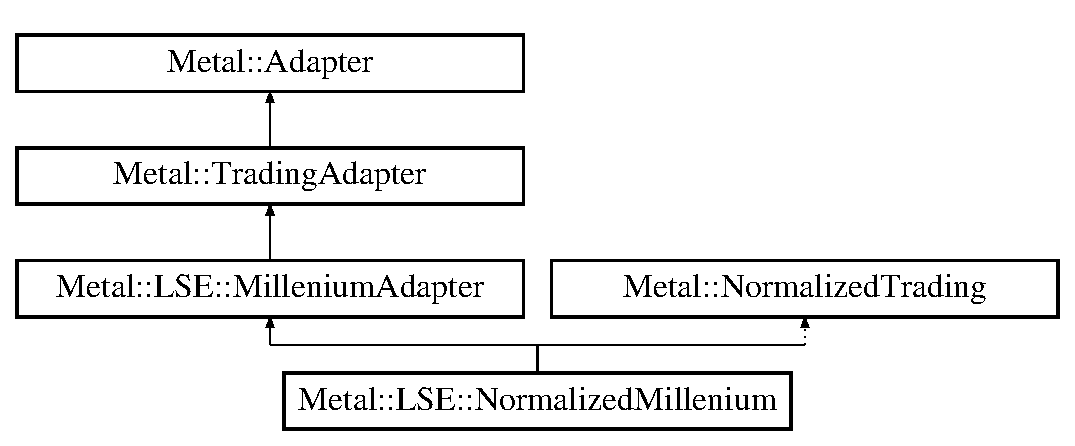
\includegraphics[height=4.000000cm]{classMetal_1_1LSE_1_1NormalizedMillenium}
\end{center}
\end{figure}
\subsection*{Public Member Functions}
\begin{DoxyCompactItemize}
\item 
\hyperlink{classMetal_1_1LSE_1_1NormalizedMillenium_a5716062f452358e985155bbbc2736fdd}{Normalized\+Millenium} (std\+::string \hyperlink{classMetal_1_1LSE_1_1MilleniumAdapter_a1c12122da30ec79f3907a82ac1847c33}{user\+Name}, std\+::string \hyperlink{classMetal_1_1LSE_1_1MilleniumAdapter_aa8120f11aac5d4825a5766d86e53e5a2}{password})
\item 
\hyperlink{classMetal_1_1LSE_1_1NormalizedMillenium_a7c5268eb2ce51a54066460651814ce64}{$\sim$\+Normalized\+Millenium} ()
\item 
void \hyperlink{classMetal_1_1LSE_1_1NormalizedMillenium_a0307ee675723035de1c9a83de1e54ead}{send\+Cancel} (const \hyperlink{classMetal_1_1OrderCancelRequest}{Metal\+::\+Order\+Cancel\+Request} \&ocr)
\item 
void \hyperlink{classMetal_1_1LSE_1_1NormalizedMillenium_a0779d0218ce1dd1b9f0381dbd16ee142}{send\+New\+Order} (const \hyperlink{classMetal_1_1NewOrderSingle}{Metal\+::\+New\+Order\+Single} \&nos)
\end{DoxyCompactItemize}
\subsection*{Protected Member Functions}
\begin{DoxyCompactItemize}
\item 
void \hyperlink{classMetal_1_1LSE_1_1NormalizedMillenium_addd777ccae3f8eefcb942238f0d8c9cf}{on\+Execution\+Report} (const \hyperlink{namespaceMetal_af4294c176f6aecf9f75e9b106b117aa1}{Metal\+::\+Execution\+Report} \&)=0
\end{DoxyCompactItemize}
\subsection*{Additional Inherited Members}


\subsection{Constructor \& Destructor Documentation}
\hypertarget{classMetal_1_1LSE_1_1NormalizedMillenium_a5716062f452358e985155bbbc2736fdd}{}\index{Metal\+::\+L\+S\+E\+::\+Normalized\+Millenium@{Metal\+::\+L\+S\+E\+::\+Normalized\+Millenium}!Normalized\+Millenium@{Normalized\+Millenium}}
\index{Normalized\+Millenium@{Normalized\+Millenium}!Metal\+::\+L\+S\+E\+::\+Normalized\+Millenium@{Metal\+::\+L\+S\+E\+::\+Normalized\+Millenium}}
\subsubsection[{Normalized\+Millenium}]{\setlength{\rightskip}{0pt plus 5cm}Metal\+::\+L\+S\+E\+::\+Normalized\+Millenium\+::\+Normalized\+Millenium (
\begin{DoxyParamCaption}
\item[{std\+::string}]{user\+Name, }
\item[{std\+::string}]{password}
\end{DoxyParamCaption}
)}\label{classMetal_1_1LSE_1_1NormalizedMillenium_a5716062f452358e985155bbbc2736fdd}
\hypertarget{classMetal_1_1LSE_1_1NormalizedMillenium_a7c5268eb2ce51a54066460651814ce64}{}\index{Metal\+::\+L\+S\+E\+::\+Normalized\+Millenium@{Metal\+::\+L\+S\+E\+::\+Normalized\+Millenium}!````~Normalized\+Millenium@{$\sim$\+Normalized\+Millenium}}
\index{````~Normalized\+Millenium@{$\sim$\+Normalized\+Millenium}!Metal\+::\+L\+S\+E\+::\+Normalized\+Millenium@{Metal\+::\+L\+S\+E\+::\+Normalized\+Millenium}}
\subsubsection[{$\sim$\+Normalized\+Millenium}]{\setlength{\rightskip}{0pt plus 5cm}Metal\+::\+L\+S\+E\+::\+Normalized\+Millenium\+::$\sim$\+Normalized\+Millenium (
\begin{DoxyParamCaption}
{}
\end{DoxyParamCaption}
)}\label{classMetal_1_1LSE_1_1NormalizedMillenium_a7c5268eb2ce51a54066460651814ce64}


\subsection{Member Function Documentation}
\hypertarget{classMetal_1_1LSE_1_1NormalizedMillenium_addd777ccae3f8eefcb942238f0d8c9cf}{}\index{Metal\+::\+L\+S\+E\+::\+Normalized\+Millenium@{Metal\+::\+L\+S\+E\+::\+Normalized\+Millenium}!on\+Execution\+Report@{on\+Execution\+Report}}
\index{on\+Execution\+Report@{on\+Execution\+Report}!Metal\+::\+L\+S\+E\+::\+Normalized\+Millenium@{Metal\+::\+L\+S\+E\+::\+Normalized\+Millenium}}
\subsubsection[{on\+Execution\+Report}]{\setlength{\rightskip}{0pt plus 5cm}void Metal\+::\+L\+S\+E\+::\+Normalized\+Millenium\+::on\+Execution\+Report (
\begin{DoxyParamCaption}
\item[{const {\bf Metal\+::\+Execution\+Report} \&}]{}
\end{DoxyParamCaption}
)\hspace{0.3cm}{\ttfamily [protected]}, {\ttfamily [pure virtual]}}\label{classMetal_1_1LSE_1_1NormalizedMillenium_addd777ccae3f8eefcb942238f0d8c9cf}
Entry point for normalized execution reports 

Implements \hyperlink{classMetal_1_1NormalizedTrading_a270f88ce9bc2dfd0d6e65cc7490a27ce}{Metal\+::\+Normalized\+Trading}.

\hypertarget{classMetal_1_1LSE_1_1NormalizedMillenium_a0307ee675723035de1c9a83de1e54ead}{}\index{Metal\+::\+L\+S\+E\+::\+Normalized\+Millenium@{Metal\+::\+L\+S\+E\+::\+Normalized\+Millenium}!send\+Cancel@{send\+Cancel}}
\index{send\+Cancel@{send\+Cancel}!Metal\+::\+L\+S\+E\+::\+Normalized\+Millenium@{Metal\+::\+L\+S\+E\+::\+Normalized\+Millenium}}
\subsubsection[{send\+Cancel}]{\setlength{\rightskip}{0pt plus 5cm}void Metal\+::\+L\+S\+E\+::\+Normalized\+Millenium\+::send\+Cancel (
\begin{DoxyParamCaption}
\item[{const {\bf Metal\+::\+Order\+Cancel\+Request} \&}]{ocr}
\end{DoxyParamCaption}
)\hspace{0.3cm}{\ttfamily [virtual]}}\label{classMetal_1_1LSE_1_1NormalizedMillenium_a0307ee675723035de1c9a83de1e54ead}
Sends a normalized cancel \begin{DoxySeeAlso}{See also}
\hyperlink{classMetal_1_1NormalizedTrading_afbc20b8631fdde2e55c28d3a26515ab4}{Normalized\+Trading\+::send\+Cancel()} 
\end{DoxySeeAlso}


Implements \hyperlink{classMetal_1_1NormalizedTrading_afbc20b8631fdde2e55c28d3a26515ab4}{Metal\+::\+Normalized\+Trading}.

\hypertarget{classMetal_1_1LSE_1_1NormalizedMillenium_a0779d0218ce1dd1b9f0381dbd16ee142}{}\index{Metal\+::\+L\+S\+E\+::\+Normalized\+Millenium@{Metal\+::\+L\+S\+E\+::\+Normalized\+Millenium}!send\+New\+Order@{send\+New\+Order}}
\index{send\+New\+Order@{send\+New\+Order}!Metal\+::\+L\+S\+E\+::\+Normalized\+Millenium@{Metal\+::\+L\+S\+E\+::\+Normalized\+Millenium}}
\subsubsection[{send\+New\+Order}]{\setlength{\rightskip}{0pt plus 5cm}void Metal\+::\+L\+S\+E\+::\+Normalized\+Millenium\+::send\+New\+Order (
\begin{DoxyParamCaption}
\item[{const {\bf Metal\+::\+New\+Order\+Single} \&}]{nos}
\end{DoxyParamCaption}
)\hspace{0.3cm}{\ttfamily [virtual]}}\label{classMetal_1_1LSE_1_1NormalizedMillenium_a0779d0218ce1dd1b9f0381dbd16ee142}
Sends a normalized new order 

Implements \hyperlink{classMetal_1_1NormalizedTrading_a900b56c2898d265326539ece79c7931a}{Metal\+::\+Normalized\+Trading}.



The documentation for this class was generated from the following files\+:\begin{DoxyCompactItemize}
\item 
/home/jc/metal/github/src/adapters/\+L\+S\+E\+Trading\+Adapter/\hyperlink{NormalizedMillenium_8h}{Normalized\+Millenium.\+h}\item 
/home/jc/metal/github/src/adapters/\+L\+S\+E\+Trading\+Adapter/\hyperlink{NormalizedMillenium_8cpp}{Normalized\+Millenium.\+cpp}\end{DoxyCompactItemize}

\hypertarget{classMetal_1_1NormalizedTrading}{}\section{Metal\+:\+:Normalized\+Trading Class Reference}
\label{classMetal_1_1NormalizedTrading}\index{Metal\+::\+Normalized\+Trading@{Metal\+::\+Normalized\+Trading}}


{\ttfamily \#include $<$Normalized\+Trading.\+h$>$}

Inheritance diagram for Metal\+:\+:Normalized\+Trading\+:\begin{figure}[H]
\begin{center}
\leavevmode
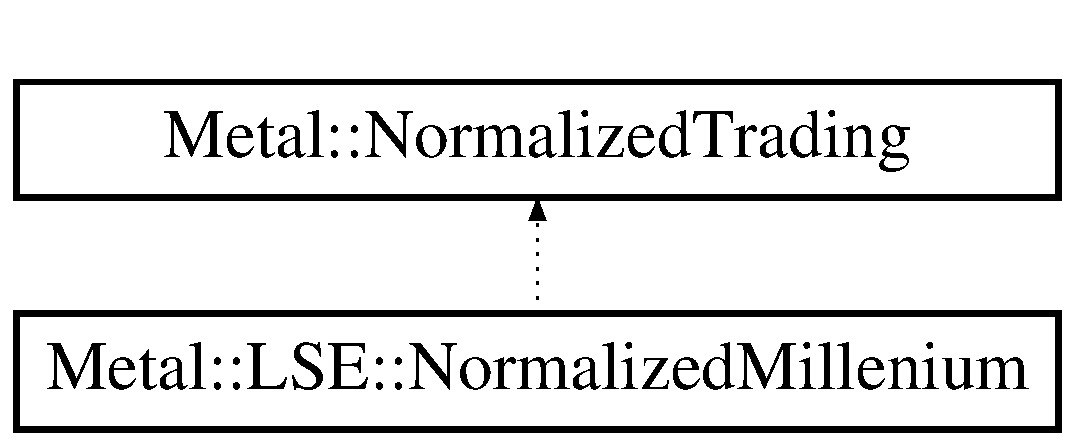
\includegraphics[height=2.000000cm]{classMetal_1_1NormalizedTrading}
\end{center}
\end{figure}
\subsection*{Public Member Functions}
\begin{DoxyCompactItemize}
\item 
\hyperlink{classMetal_1_1NormalizedTrading_ae307873f365b0d321076c8c3967a0fbd}{Normalized\+Trading} ()
\item 
virtual void \hyperlink{classMetal_1_1NormalizedTrading_afbc20b8631fdde2e55c28d3a26515ab4}{send\+Cancel} (const \hyperlink{classMetal_1_1OrderCancelRequest}{Order\+Cancel\+Request} \&)=0
\item 
virtual void \hyperlink{classMetal_1_1NormalizedTrading_a900b56c2898d265326539ece79c7931a}{send\+New\+Order} (const \hyperlink{classMetal_1_1NewOrderSingle}{New\+Order\+Single} \&)=0
\end{DoxyCompactItemize}
\subsection*{Protected Member Functions}
\begin{DoxyCompactItemize}
\item 
\hyperlink{classMetal_1_1NormalizedTrading_a6abc2cf93b45831969d3ea67bcdb2932}{$\sim$\+Normalized\+Trading} ()
\item 
virtual void \hyperlink{classMetal_1_1NormalizedTrading_a270f88ce9bc2dfd0d6e65cc7490a27ce}{on\+Execution\+Report} (const \hyperlink{namespaceMetal_af4294c176f6aecf9f75e9b106b117aa1}{Execution\+Report} \&)=0
\end{DoxyCompactItemize}


\subsection{Detailed Description}
\hyperlink{classMetal_1_1TradingAdapter}{Trading\+Adapter} responsibility~\newline
 1) Send New Orders, Receive execution reports 

\subsection{Constructor \& Destructor Documentation}
\hypertarget{classMetal_1_1NormalizedTrading_ae307873f365b0d321076c8c3967a0fbd}{}\index{Metal\+::\+Normalized\+Trading@{Metal\+::\+Normalized\+Trading}!Normalized\+Trading@{Normalized\+Trading}}
\index{Normalized\+Trading@{Normalized\+Trading}!Metal\+::\+Normalized\+Trading@{Metal\+::\+Normalized\+Trading}}
\subsubsection[{Normalized\+Trading}]{\setlength{\rightskip}{0pt plus 5cm}Metal\+::\+Normalized\+Trading\+::\+Normalized\+Trading (
\begin{DoxyParamCaption}
{}
\end{DoxyParamCaption}
)\hspace{0.3cm}{\ttfamily [inline]}}\label{classMetal_1_1NormalizedTrading_ae307873f365b0d321076c8c3967a0fbd}
\hypertarget{classMetal_1_1NormalizedTrading_a6abc2cf93b45831969d3ea67bcdb2932}{}\index{Metal\+::\+Normalized\+Trading@{Metal\+::\+Normalized\+Trading}!````~Normalized\+Trading@{$\sim$\+Normalized\+Trading}}
\index{````~Normalized\+Trading@{$\sim$\+Normalized\+Trading}!Metal\+::\+Normalized\+Trading@{Metal\+::\+Normalized\+Trading}}
\subsubsection[{$\sim$\+Normalized\+Trading}]{\setlength{\rightskip}{0pt plus 5cm}Metal\+::\+Normalized\+Trading\+::$\sim$\+Normalized\+Trading (
\begin{DoxyParamCaption}
{}
\end{DoxyParamCaption}
)\hspace{0.3cm}{\ttfamily [inline]}, {\ttfamily [protected]}}\label{classMetal_1_1NormalizedTrading_a6abc2cf93b45831969d3ea67bcdb2932}


\subsection{Member Function Documentation}
\hypertarget{classMetal_1_1NormalizedTrading_a270f88ce9bc2dfd0d6e65cc7490a27ce}{}\index{Metal\+::\+Normalized\+Trading@{Metal\+::\+Normalized\+Trading}!on\+Execution\+Report@{on\+Execution\+Report}}
\index{on\+Execution\+Report@{on\+Execution\+Report}!Metal\+::\+Normalized\+Trading@{Metal\+::\+Normalized\+Trading}}
\subsubsection[{on\+Execution\+Report}]{\setlength{\rightskip}{0pt plus 5cm}virtual void Metal\+::\+Normalized\+Trading\+::on\+Execution\+Report (
\begin{DoxyParamCaption}
\item[{const {\bf Execution\+Report} \&}]{}
\end{DoxyParamCaption}
)\hspace{0.3cm}{\ttfamily [protected]}, {\ttfamily [pure virtual]}}\label{classMetal_1_1NormalizedTrading_a270f88ce9bc2dfd0d6e65cc7490a27ce}
Entry point for every execution reports 

Implemented in \hyperlink{classMetal_1_1LSE_1_1NormalizedMillenium_addd777ccae3f8eefcb942238f0d8c9cf}{Metal\+::\+L\+S\+E\+::\+Normalized\+Millenium}.

\hypertarget{classMetal_1_1NormalizedTrading_afbc20b8631fdde2e55c28d3a26515ab4}{}\index{Metal\+::\+Normalized\+Trading@{Metal\+::\+Normalized\+Trading}!send\+Cancel@{send\+Cancel}}
\index{send\+Cancel@{send\+Cancel}!Metal\+::\+Normalized\+Trading@{Metal\+::\+Normalized\+Trading}}
\subsubsection[{send\+Cancel}]{\setlength{\rightskip}{0pt plus 5cm}virtual void Metal\+::\+Normalized\+Trading\+::send\+Cancel (
\begin{DoxyParamCaption}
\item[{const {\bf Order\+Cancel\+Request} \&}]{}
\end{DoxyParamCaption}
)\hspace{0.3cm}{\ttfamily [pure virtual]}}\label{classMetal_1_1NormalizedTrading_afbc20b8631fdde2e55c28d3a26515ab4}
Formats and sends a normalized Order Cancel Request 

Implemented in \hyperlink{classMetal_1_1LSE_1_1NormalizedMillenium_a0307ee675723035de1c9a83de1e54ead}{Metal\+::\+L\+S\+E\+::\+Normalized\+Millenium}.

\hypertarget{classMetal_1_1NormalizedTrading_a900b56c2898d265326539ece79c7931a}{}\index{Metal\+::\+Normalized\+Trading@{Metal\+::\+Normalized\+Trading}!send\+New\+Order@{send\+New\+Order}}
\index{send\+New\+Order@{send\+New\+Order}!Metal\+::\+Normalized\+Trading@{Metal\+::\+Normalized\+Trading}}
\subsubsection[{send\+New\+Order}]{\setlength{\rightskip}{0pt plus 5cm}virtual void Metal\+::\+Normalized\+Trading\+::send\+New\+Order (
\begin{DoxyParamCaption}
\item[{const {\bf New\+Order\+Single} \&}]{}
\end{DoxyParamCaption}
)\hspace{0.3cm}{\ttfamily [pure virtual]}}\label{classMetal_1_1NormalizedTrading_a900b56c2898d265326539ece79c7931a}
This method will be called by users to send new orders~\newline
 It should map from generic to specific format then encode and send~\newline
 
\begin{DoxyParams}{Parameters}
{\em \hyperlink{classMetal_1_1NewOrderSingle}{New\+Order\+Single}} & Inbound order in unified format \\
\hline
\end{DoxyParams}
\begin{DoxySeeAlso}{See also}
\hyperlink{classMetal_1_1NewOrderSingle}{New\+Order\+Single} 
\end{DoxySeeAlso}


Implemented in \hyperlink{classMetal_1_1LSE_1_1NormalizedMillenium_a0779d0218ce1dd1b9f0381dbd16ee142}{Metal\+::\+L\+S\+E\+::\+Normalized\+Millenium}.



The documentation for this class was generated from the following file\+:\begin{DoxyCompactItemize}
\item 
/home/jc/metal/github/include/metal/\hyperlink{NormalizedTrading_8h}{Normalized\+Trading.\+h}\end{DoxyCompactItemize}

\hypertarget{classMetal_1_1Aquis_1_1OrderAdd}{}\section{Metal\+:\+:Aquis\+:\+:Order\+Add Class Reference}
\label{classMetal_1_1Aquis_1_1OrderAdd}\index{Metal\+::\+Aquis\+::\+Order\+Add@{Metal\+::\+Aquis\+::\+Order\+Add}}


{\ttfamily \#include $<$Order\+Add.\+h$>$}

\subsection*{Public Member Functions}
\begin{DoxyCompactItemize}
\item 
\hyperlink{classMetal_1_1Aquis_1_1OrderAdd_a019321c8f9ec0df43faabeb55f7eb0e3}{Order\+Add} ()
\item 
virtual \hyperlink{classMetal_1_1Aquis_1_1OrderAdd_ae5878f9b73b48d8d1b3f135e7fe24eb2}{$\sim$\+Order\+Add} ()
\end{DoxyCompactItemize}
\subsection*{Public Attributes}
\begin{DoxyCompactItemize}
\item 
\hyperlink{namespaceMetal_1_1Aquis_a822c1f3c19e277e264ba31d810cadbea}{Security\+Id} \hyperlink{classMetal_1_1Aquis_1_1OrderAdd_a52d6147f00cb5093553e2371e0889128}{security\+Id}
\item 
\hyperlink{namespaceMetal_1_1Aquis_aedaac80110efc9b37a08e697501250ba}{Order\+Type} \hyperlink{classMetal_1_1Aquis_1_1OrderAdd_a1b9869d70224141118898b0892282e43}{order\+Type}
\item 
\hyperlink{namespaceMetal_1_1Aquis_afb13b4ac40f6f0b4f0085bfd9572b42d}{Time\+In\+Force} \hyperlink{classMetal_1_1Aquis_1_1OrderAdd_aee9ffdefdcf5f575c2c1228627e89430}{timein\+Force}
\item 
\hyperlink{namespaceMetal_1_1Aquis_ae45bfb9f528bd35d5f31d9ba1b9eafcf}{Side} \hyperlink{classMetal_1_1Aquis_1_1OrderAdd_a434dd763ee773caacf674f03ff4d54d8}{side}
\item 
\hyperlink{namespaceMetal_1_1Aquis_aa25d3bf823ec854f4e93eee2c5f0b529}{Quantity} \hyperlink{classMetal_1_1Aquis_1_1OrderAdd_a2643463679c661d8dab941c3f2bf40fe}{quantity}
\item 
\hyperlink{namespaceMetal_1_1Aquis_a83ca009113cb4fca87827adfee66bcbd}{Price} \hyperlink{classMetal_1_1Aquis_1_1OrderAdd_afe71fd701739a64aaf3c0ed52fe4fcb3}{price}
\item 
\hyperlink{namespaceMetal_1_1Aquis_ac8ffebbdb8def9d93b29ba3fc6878e09}{Order\+Capacity} \hyperlink{classMetal_1_1Aquis_1_1OrderAdd_a6d33517e78c0d5aa0959cc0ef75aaeb0}{order\+Capacity}
\item 
\hyperlink{namespaceMetal_1_1Aquis_acbe82ae737d4c087f18f1af8aabd1d26}{Account} \hyperlink{classMetal_1_1Aquis_1_1OrderAdd_a9c0c3b2e0c4aa5c96b84a9d7bddd980a}{account}
\item 
\hyperlink{namespaceMetal_1_1Aquis_a9e7c42d4dce76e920bc18eb66b799cf4}{User\+Tag} \hyperlink{classMetal_1_1Aquis_1_1OrderAdd_ac81fd314fe475edf236c36f47764cc72}{user\+Tag}
\end{DoxyCompactItemize}


\subsection{Constructor \& Destructor Documentation}
\hypertarget{classMetal_1_1Aquis_1_1OrderAdd_a019321c8f9ec0df43faabeb55f7eb0e3}{}\index{Metal\+::\+Aquis\+::\+Order\+Add@{Metal\+::\+Aquis\+::\+Order\+Add}!Order\+Add@{Order\+Add}}
\index{Order\+Add@{Order\+Add}!Metal\+::\+Aquis\+::\+Order\+Add@{Metal\+::\+Aquis\+::\+Order\+Add}}
\subsubsection[{Order\+Add}]{\setlength{\rightskip}{0pt plus 5cm}Metal\+::\+Aquis\+::\+Order\+Add\+::\+Order\+Add (
\begin{DoxyParamCaption}
{}
\end{DoxyParamCaption}
)}\label{classMetal_1_1Aquis_1_1OrderAdd_a019321c8f9ec0df43faabeb55f7eb0e3}
\hypertarget{classMetal_1_1Aquis_1_1OrderAdd_ae5878f9b73b48d8d1b3f135e7fe24eb2}{}\index{Metal\+::\+Aquis\+::\+Order\+Add@{Metal\+::\+Aquis\+::\+Order\+Add}!````~Order\+Add@{$\sim$\+Order\+Add}}
\index{````~Order\+Add@{$\sim$\+Order\+Add}!Metal\+::\+Aquis\+::\+Order\+Add@{Metal\+::\+Aquis\+::\+Order\+Add}}
\subsubsection[{$\sim$\+Order\+Add}]{\setlength{\rightskip}{0pt plus 5cm}Metal\+::\+Aquis\+::\+Order\+Add\+::$\sim$\+Order\+Add (
\begin{DoxyParamCaption}
{}
\end{DoxyParamCaption}
)\hspace{0.3cm}{\ttfamily [virtual]}}\label{classMetal_1_1Aquis_1_1OrderAdd_ae5878f9b73b48d8d1b3f135e7fe24eb2}


\subsection{Member Data Documentation}
\hypertarget{classMetal_1_1Aquis_1_1OrderAdd_a9c0c3b2e0c4aa5c96b84a9d7bddd980a}{}\index{Metal\+::\+Aquis\+::\+Order\+Add@{Metal\+::\+Aquis\+::\+Order\+Add}!account@{account}}
\index{account@{account}!Metal\+::\+Aquis\+::\+Order\+Add@{Metal\+::\+Aquis\+::\+Order\+Add}}
\subsubsection[{account}]{\setlength{\rightskip}{0pt plus 5cm}{\bf Account} Metal\+::\+Aquis\+::\+Order\+Add\+::account}\label{classMetal_1_1Aquis_1_1OrderAdd_a9c0c3b2e0c4aa5c96b84a9d7bddd980a}
\hypertarget{classMetal_1_1Aquis_1_1OrderAdd_a6d33517e78c0d5aa0959cc0ef75aaeb0}{}\index{Metal\+::\+Aquis\+::\+Order\+Add@{Metal\+::\+Aquis\+::\+Order\+Add}!order\+Capacity@{order\+Capacity}}
\index{order\+Capacity@{order\+Capacity}!Metal\+::\+Aquis\+::\+Order\+Add@{Metal\+::\+Aquis\+::\+Order\+Add}}
\subsubsection[{order\+Capacity}]{\setlength{\rightskip}{0pt plus 5cm}{\bf Order\+Capacity} Metal\+::\+Aquis\+::\+Order\+Add\+::order\+Capacity}\label{classMetal_1_1Aquis_1_1OrderAdd_a6d33517e78c0d5aa0959cc0ef75aaeb0}
\hypertarget{classMetal_1_1Aquis_1_1OrderAdd_a1b9869d70224141118898b0892282e43}{}\index{Metal\+::\+Aquis\+::\+Order\+Add@{Metal\+::\+Aquis\+::\+Order\+Add}!order\+Type@{order\+Type}}
\index{order\+Type@{order\+Type}!Metal\+::\+Aquis\+::\+Order\+Add@{Metal\+::\+Aquis\+::\+Order\+Add}}
\subsubsection[{order\+Type}]{\setlength{\rightskip}{0pt plus 5cm}{\bf Order\+Type} Metal\+::\+Aquis\+::\+Order\+Add\+::order\+Type}\label{classMetal_1_1Aquis_1_1OrderAdd_a1b9869d70224141118898b0892282e43}
\hypertarget{classMetal_1_1Aquis_1_1OrderAdd_afe71fd701739a64aaf3c0ed52fe4fcb3}{}\index{Metal\+::\+Aquis\+::\+Order\+Add@{Metal\+::\+Aquis\+::\+Order\+Add}!price@{price}}
\index{price@{price}!Metal\+::\+Aquis\+::\+Order\+Add@{Metal\+::\+Aquis\+::\+Order\+Add}}
\subsubsection[{price}]{\setlength{\rightskip}{0pt plus 5cm}{\bf Price} Metal\+::\+Aquis\+::\+Order\+Add\+::price}\label{classMetal_1_1Aquis_1_1OrderAdd_afe71fd701739a64aaf3c0ed52fe4fcb3}
\hypertarget{classMetal_1_1Aquis_1_1OrderAdd_a2643463679c661d8dab941c3f2bf40fe}{}\index{Metal\+::\+Aquis\+::\+Order\+Add@{Metal\+::\+Aquis\+::\+Order\+Add}!quantity@{quantity}}
\index{quantity@{quantity}!Metal\+::\+Aquis\+::\+Order\+Add@{Metal\+::\+Aquis\+::\+Order\+Add}}
\subsubsection[{quantity}]{\setlength{\rightskip}{0pt plus 5cm}{\bf Quantity} Metal\+::\+Aquis\+::\+Order\+Add\+::quantity}\label{classMetal_1_1Aquis_1_1OrderAdd_a2643463679c661d8dab941c3f2bf40fe}
\hypertarget{classMetal_1_1Aquis_1_1OrderAdd_a52d6147f00cb5093553e2371e0889128}{}\index{Metal\+::\+Aquis\+::\+Order\+Add@{Metal\+::\+Aquis\+::\+Order\+Add}!security\+Id@{security\+Id}}
\index{security\+Id@{security\+Id}!Metal\+::\+Aquis\+::\+Order\+Add@{Metal\+::\+Aquis\+::\+Order\+Add}}
\subsubsection[{security\+Id}]{\setlength{\rightskip}{0pt plus 5cm}{\bf Security\+Id} Metal\+::\+Aquis\+::\+Order\+Add\+::security\+Id}\label{classMetal_1_1Aquis_1_1OrderAdd_a52d6147f00cb5093553e2371e0889128}
\hypertarget{classMetal_1_1Aquis_1_1OrderAdd_a434dd763ee773caacf674f03ff4d54d8}{}\index{Metal\+::\+Aquis\+::\+Order\+Add@{Metal\+::\+Aquis\+::\+Order\+Add}!side@{side}}
\index{side@{side}!Metal\+::\+Aquis\+::\+Order\+Add@{Metal\+::\+Aquis\+::\+Order\+Add}}
\subsubsection[{side}]{\setlength{\rightskip}{0pt plus 5cm}{\bf Side} Metal\+::\+Aquis\+::\+Order\+Add\+::side}\label{classMetal_1_1Aquis_1_1OrderAdd_a434dd763ee773caacf674f03ff4d54d8}
\hypertarget{classMetal_1_1Aquis_1_1OrderAdd_aee9ffdefdcf5f575c2c1228627e89430}{}\index{Metal\+::\+Aquis\+::\+Order\+Add@{Metal\+::\+Aquis\+::\+Order\+Add}!timein\+Force@{timein\+Force}}
\index{timein\+Force@{timein\+Force}!Metal\+::\+Aquis\+::\+Order\+Add@{Metal\+::\+Aquis\+::\+Order\+Add}}
\subsubsection[{timein\+Force}]{\setlength{\rightskip}{0pt plus 5cm}{\bf Time\+In\+Force} Metal\+::\+Aquis\+::\+Order\+Add\+::timein\+Force}\label{classMetal_1_1Aquis_1_1OrderAdd_aee9ffdefdcf5f575c2c1228627e89430}
\hypertarget{classMetal_1_1Aquis_1_1OrderAdd_ac81fd314fe475edf236c36f47764cc72}{}\index{Metal\+::\+Aquis\+::\+Order\+Add@{Metal\+::\+Aquis\+::\+Order\+Add}!user\+Tag@{user\+Tag}}
\index{user\+Tag@{user\+Tag}!Metal\+::\+Aquis\+::\+Order\+Add@{Metal\+::\+Aquis\+::\+Order\+Add}}
\subsubsection[{user\+Tag}]{\setlength{\rightskip}{0pt plus 5cm}{\bf User\+Tag} Metal\+::\+Aquis\+::\+Order\+Add\+::user\+Tag}\label{classMetal_1_1Aquis_1_1OrderAdd_ac81fd314fe475edf236c36f47764cc72}


The documentation for this class was generated from the following files\+:\begin{DoxyCompactItemize}
\item 
/home/jc/metal/github/src/adapters/\+Aquis\+A\+T\+P\+Adapter/\hyperlink{OrderAdd_8h}{Order\+Add.\+h}\item 
/home/jc/metal/github/src/adapters/\+Aquis\+A\+T\+P\+Adapter/\hyperlink{OrderAdd_8cpp}{Order\+Add.\+cpp}\end{DoxyCompactItemize}

\hypertarget{classMetal_1_1Aquis_1_1OrderCancel}{}\section{Metal\+:\+:Aquis\+:\+:Order\+Cancel Class Reference}
\label{classMetal_1_1Aquis_1_1OrderCancel}\index{Metal\+::\+Aquis\+::\+Order\+Cancel@{Metal\+::\+Aquis\+::\+Order\+Cancel}}


{\ttfamily \#include $<$Order\+Cancel.\+h$>$}

\subsection*{Public Member Functions}
\begin{DoxyCompactItemize}
\item 
\hyperlink{classMetal_1_1Aquis_1_1OrderCancel_aaf900b9f44b55b631b1dd7a93322784b}{Order\+Cancel} ()
\item 
virtual \hyperlink{classMetal_1_1Aquis_1_1OrderCancel_aee5afe51f2e543c2ec45998126608f50}{$\sim$\+Order\+Cancel} ()
\end{DoxyCompactItemize}
\subsection*{Public Attributes}
\begin{DoxyCompactItemize}
\item 
\hyperlink{namespaceMetal_1_1Aquis_a9d9056c8752e245df5a2c554ce6d3d1a}{Order\+Ref} \hyperlink{classMetal_1_1Aquis_1_1OrderCancel_a7b4ac3d47774e8c17f79ff1f2b51d8f8}{order\+Ref}
\item 
\hyperlink{namespaceMetal_1_1Aquis_a9e7c42d4dce76e920bc18eb66b799cf4}{User\+Tag} \hyperlink{classMetal_1_1Aquis_1_1OrderCancel_a0b004bfa7f710dd8d57220695e2aa1f5}{user\+Tag}
\end{DoxyCompactItemize}


\subsection{Constructor \& Destructor Documentation}
\hypertarget{classMetal_1_1Aquis_1_1OrderCancel_aaf900b9f44b55b631b1dd7a93322784b}{}\index{Metal\+::\+Aquis\+::\+Order\+Cancel@{Metal\+::\+Aquis\+::\+Order\+Cancel}!Order\+Cancel@{Order\+Cancel}}
\index{Order\+Cancel@{Order\+Cancel}!Metal\+::\+Aquis\+::\+Order\+Cancel@{Metal\+::\+Aquis\+::\+Order\+Cancel}}
\subsubsection[{Order\+Cancel}]{\setlength{\rightskip}{0pt plus 5cm}Metal\+::\+Aquis\+::\+Order\+Cancel\+::\+Order\+Cancel (
\begin{DoxyParamCaption}
{}
\end{DoxyParamCaption}
)}\label{classMetal_1_1Aquis_1_1OrderCancel_aaf900b9f44b55b631b1dd7a93322784b}
\hypertarget{classMetal_1_1Aquis_1_1OrderCancel_aee5afe51f2e543c2ec45998126608f50}{}\index{Metal\+::\+Aquis\+::\+Order\+Cancel@{Metal\+::\+Aquis\+::\+Order\+Cancel}!````~Order\+Cancel@{$\sim$\+Order\+Cancel}}
\index{````~Order\+Cancel@{$\sim$\+Order\+Cancel}!Metal\+::\+Aquis\+::\+Order\+Cancel@{Metal\+::\+Aquis\+::\+Order\+Cancel}}
\subsubsection[{$\sim$\+Order\+Cancel}]{\setlength{\rightskip}{0pt plus 5cm}Metal\+::\+Aquis\+::\+Order\+Cancel\+::$\sim$\+Order\+Cancel (
\begin{DoxyParamCaption}
{}
\end{DoxyParamCaption}
)\hspace{0.3cm}{\ttfamily [virtual]}}\label{classMetal_1_1Aquis_1_1OrderCancel_aee5afe51f2e543c2ec45998126608f50}


\subsection{Member Data Documentation}
\hypertarget{classMetal_1_1Aquis_1_1OrderCancel_a7b4ac3d47774e8c17f79ff1f2b51d8f8}{}\index{Metal\+::\+Aquis\+::\+Order\+Cancel@{Metal\+::\+Aquis\+::\+Order\+Cancel}!order\+Ref@{order\+Ref}}
\index{order\+Ref@{order\+Ref}!Metal\+::\+Aquis\+::\+Order\+Cancel@{Metal\+::\+Aquis\+::\+Order\+Cancel}}
\subsubsection[{order\+Ref}]{\setlength{\rightskip}{0pt plus 5cm}{\bf Order\+Ref} Metal\+::\+Aquis\+::\+Order\+Cancel\+::order\+Ref}\label{classMetal_1_1Aquis_1_1OrderCancel_a7b4ac3d47774e8c17f79ff1f2b51d8f8}
\hypertarget{classMetal_1_1Aquis_1_1OrderCancel_a0b004bfa7f710dd8d57220695e2aa1f5}{}\index{Metal\+::\+Aquis\+::\+Order\+Cancel@{Metal\+::\+Aquis\+::\+Order\+Cancel}!user\+Tag@{user\+Tag}}
\index{user\+Tag@{user\+Tag}!Metal\+::\+Aquis\+::\+Order\+Cancel@{Metal\+::\+Aquis\+::\+Order\+Cancel}}
\subsubsection[{user\+Tag}]{\setlength{\rightskip}{0pt plus 5cm}{\bf User\+Tag} Metal\+::\+Aquis\+::\+Order\+Cancel\+::user\+Tag}\label{classMetal_1_1Aquis_1_1OrderCancel_a0b004bfa7f710dd8d57220695e2aa1f5}


The documentation for this class was generated from the following files\+:\begin{DoxyCompactItemize}
\item 
/home/jc/metal/github/src/adapters/\+Aquis\+A\+T\+P\+Adapter/\hyperlink{OrderCancel_8h}{Order\+Cancel.\+h}\item 
/home/jc/metal/github/src/adapters/\+Aquis\+A\+T\+P\+Adapter/\hyperlink{OrderCancel_8cpp}{Order\+Cancel.\+cpp}\end{DoxyCompactItemize}

\hypertarget{classMetal_1_1OrderCancelRequest}{}\section{Metal\+:\+:Order\+Cancel\+Request Class Reference}
\label{classMetal_1_1OrderCancelRequest}\index{Metal\+::\+Order\+Cancel\+Request@{Metal\+::\+Order\+Cancel\+Request}}


{\ttfamily \#include $<$metal.\+h$>$}

Inheritance diagram for Metal\+:\+:Order\+Cancel\+Request\+:\begin{figure}[H]
\begin{center}
\leavevmode
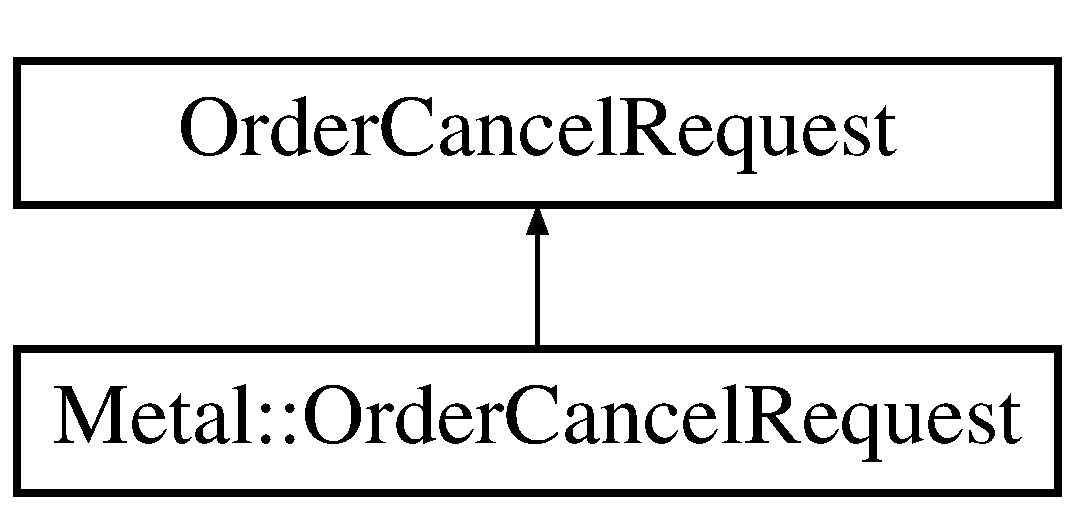
\includegraphics[height=2.000000cm]{classMetal_1_1OrderCancelRequest}
\end{center}
\end{figure}


The documentation for this class was generated from the following file\+:\begin{DoxyCompactItemize}
\item 
/home/jc/metal/github/include/metal/\hyperlink{metal_8h}{metal.\+h}\end{DoxyCompactItemize}

\hypertarget{classMetal_1_1LSE_1_1OrderCancelRequest}{}\section{Metal\+:\+:L\+S\+E\+:\+:Order\+Cancel\+Request Class Reference}
\label{classMetal_1_1LSE_1_1OrderCancelRequest}\index{Metal\+::\+L\+S\+E\+::\+Order\+Cancel\+Request@{Metal\+::\+L\+S\+E\+::\+Order\+Cancel\+Request}}


{\ttfamily \#include $<$Order\+Cancel\+Request.\+h$>$}

Inheritance diagram for Metal\+:\+:L\+S\+E\+:\+:Order\+Cancel\+Request\+:\begin{figure}[H]
\begin{center}
\leavevmode
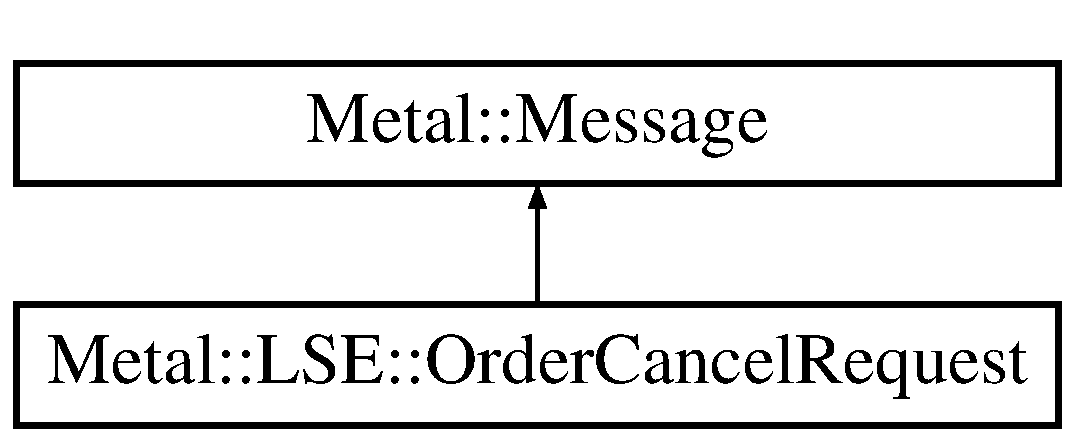
\includegraphics[height=2.000000cm]{classMetal_1_1LSE_1_1OrderCancelRequest}
\end{center}
\end{figure}
\subsection*{Public Member Functions}
\begin{DoxyCompactItemize}
\item 
\hyperlink{classMetal_1_1LSE_1_1OrderCancelRequest_a7334bf6b9c759c5d9c493fba0507111d}{Order\+Cancel\+Request} ()
\item 
virtual \hyperlink{classMetal_1_1LSE_1_1OrderCancelRequest_ada763ff79958a669d9255d8eb2028b60}{$\sim$\+Order\+Cancel\+Request} ()
\end{DoxyCompactItemize}
\subsection*{Public Attributes}
\begin{DoxyCompactItemize}
\item 
\hyperlink{namespaceMetal_1_1LSE_a7f5f027430e2d08dcf1a5ccba4ea7bc6}{Client\+Order\+I\+D} \hyperlink{classMetal_1_1LSE_1_1OrderCancelRequest_a17cf42a99f70826442cd78668a20e460}{client\+Order\+I\+D}
\item 
\hyperlink{namespaceMetal_1_1LSE_af5236b7a999484d8cd5b579b7d7c133b}{Side} \hyperlink{classMetal_1_1LSE_1_1OrderCancelRequest_a8147911f2234bdb988adfb6f43b7aaca}{side}
\item 
\hyperlink{namespaceMetal_1_1LSE_a30b8c9f132779cac1a35919835725059}{Order\+I\+D} \hyperlink{classMetal_1_1LSE_1_1OrderCancelRequest_ad35bf5f0e86e582724e8e6868028b976}{order\+Id}
\item 
\hyperlink{namespaceMetal_1_1LSE_a28d9de72a77b3eab8551831696a678c1}{Original\+Client\+Order\+I\+D} \hyperlink{classMetal_1_1LSE_1_1OrderCancelRequest_a96b6730c82337371d5de0354566a616c}{original\+Client\+Order\+Id}
\item 
\hyperlink{namespaceMetal_1_1LSE_a5280aa41aaa4433df351e733a23ecd14}{Instrument\+I\+D} \hyperlink{classMetal_1_1LSE_1_1OrderCancelRequest_a25a35022d18a4c0826199bbb6950ad16}{instrument\+I\+D}
\end{DoxyCompactItemize}
\subsection*{Additional Inherited Members}


\subsection{Constructor \& Destructor Documentation}
\hypertarget{classMetal_1_1LSE_1_1OrderCancelRequest_a7334bf6b9c759c5d9c493fba0507111d}{}\index{Metal\+::\+L\+S\+E\+::\+Order\+Cancel\+Request@{Metal\+::\+L\+S\+E\+::\+Order\+Cancel\+Request}!Order\+Cancel\+Request@{Order\+Cancel\+Request}}
\index{Order\+Cancel\+Request@{Order\+Cancel\+Request}!Metal\+::\+L\+S\+E\+::\+Order\+Cancel\+Request@{Metal\+::\+L\+S\+E\+::\+Order\+Cancel\+Request}}
\subsubsection[{Order\+Cancel\+Request}]{\setlength{\rightskip}{0pt plus 5cm}Metal\+::\+L\+S\+E\+::\+Order\+Cancel\+Request\+::\+Order\+Cancel\+Request (
\begin{DoxyParamCaption}
{}
\end{DoxyParamCaption}
)}\label{classMetal_1_1LSE_1_1OrderCancelRequest_a7334bf6b9c759c5d9c493fba0507111d}
\hypertarget{classMetal_1_1LSE_1_1OrderCancelRequest_ada763ff79958a669d9255d8eb2028b60}{}\index{Metal\+::\+L\+S\+E\+::\+Order\+Cancel\+Request@{Metal\+::\+L\+S\+E\+::\+Order\+Cancel\+Request}!````~Order\+Cancel\+Request@{$\sim$\+Order\+Cancel\+Request}}
\index{````~Order\+Cancel\+Request@{$\sim$\+Order\+Cancel\+Request}!Metal\+::\+L\+S\+E\+::\+Order\+Cancel\+Request@{Metal\+::\+L\+S\+E\+::\+Order\+Cancel\+Request}}
\subsubsection[{$\sim$\+Order\+Cancel\+Request}]{\setlength{\rightskip}{0pt plus 5cm}Metal\+::\+L\+S\+E\+::\+Order\+Cancel\+Request\+::$\sim$\+Order\+Cancel\+Request (
\begin{DoxyParamCaption}
{}
\end{DoxyParamCaption}
)\hspace{0.3cm}{\ttfamily [virtual]}}\label{classMetal_1_1LSE_1_1OrderCancelRequest_ada763ff79958a669d9255d8eb2028b60}


\subsection{Member Data Documentation}
\hypertarget{classMetal_1_1LSE_1_1OrderCancelRequest_a17cf42a99f70826442cd78668a20e460}{}\index{Metal\+::\+L\+S\+E\+::\+Order\+Cancel\+Request@{Metal\+::\+L\+S\+E\+::\+Order\+Cancel\+Request}!client\+Order\+I\+D@{client\+Order\+I\+D}}
\index{client\+Order\+I\+D@{client\+Order\+I\+D}!Metal\+::\+L\+S\+E\+::\+Order\+Cancel\+Request@{Metal\+::\+L\+S\+E\+::\+Order\+Cancel\+Request}}
\subsubsection[{client\+Order\+I\+D}]{\setlength{\rightskip}{0pt plus 5cm}{\bf Client\+Order\+I\+D} Metal\+::\+L\+S\+E\+::\+Order\+Cancel\+Request\+::client\+Order\+I\+D}\label{classMetal_1_1LSE_1_1OrderCancelRequest_a17cf42a99f70826442cd78668a20e460}
\hypertarget{classMetal_1_1LSE_1_1OrderCancelRequest_a25a35022d18a4c0826199bbb6950ad16}{}\index{Metal\+::\+L\+S\+E\+::\+Order\+Cancel\+Request@{Metal\+::\+L\+S\+E\+::\+Order\+Cancel\+Request}!instrument\+I\+D@{instrument\+I\+D}}
\index{instrument\+I\+D@{instrument\+I\+D}!Metal\+::\+L\+S\+E\+::\+Order\+Cancel\+Request@{Metal\+::\+L\+S\+E\+::\+Order\+Cancel\+Request}}
\subsubsection[{instrument\+I\+D}]{\setlength{\rightskip}{0pt plus 5cm}{\bf Instrument\+I\+D} Metal\+::\+L\+S\+E\+::\+Order\+Cancel\+Request\+::instrument\+I\+D}\label{classMetal_1_1LSE_1_1OrderCancelRequest_a25a35022d18a4c0826199bbb6950ad16}
\hypertarget{classMetal_1_1LSE_1_1OrderCancelRequest_ad35bf5f0e86e582724e8e6868028b976}{}\index{Metal\+::\+L\+S\+E\+::\+Order\+Cancel\+Request@{Metal\+::\+L\+S\+E\+::\+Order\+Cancel\+Request}!order\+Id@{order\+Id}}
\index{order\+Id@{order\+Id}!Metal\+::\+L\+S\+E\+::\+Order\+Cancel\+Request@{Metal\+::\+L\+S\+E\+::\+Order\+Cancel\+Request}}
\subsubsection[{order\+Id}]{\setlength{\rightskip}{0pt plus 5cm}{\bf Order\+I\+D} Metal\+::\+L\+S\+E\+::\+Order\+Cancel\+Request\+::order\+Id}\label{classMetal_1_1LSE_1_1OrderCancelRequest_ad35bf5f0e86e582724e8e6868028b976}
\hypertarget{classMetal_1_1LSE_1_1OrderCancelRequest_a96b6730c82337371d5de0354566a616c}{}\index{Metal\+::\+L\+S\+E\+::\+Order\+Cancel\+Request@{Metal\+::\+L\+S\+E\+::\+Order\+Cancel\+Request}!original\+Client\+Order\+Id@{original\+Client\+Order\+Id}}
\index{original\+Client\+Order\+Id@{original\+Client\+Order\+Id}!Metal\+::\+L\+S\+E\+::\+Order\+Cancel\+Request@{Metal\+::\+L\+S\+E\+::\+Order\+Cancel\+Request}}
\subsubsection[{original\+Client\+Order\+Id}]{\setlength{\rightskip}{0pt plus 5cm}{\bf Original\+Client\+Order\+I\+D} Metal\+::\+L\+S\+E\+::\+Order\+Cancel\+Request\+::original\+Client\+Order\+Id}\label{classMetal_1_1LSE_1_1OrderCancelRequest_a96b6730c82337371d5de0354566a616c}
\hypertarget{classMetal_1_1LSE_1_1OrderCancelRequest_a8147911f2234bdb988adfb6f43b7aaca}{}\index{Metal\+::\+L\+S\+E\+::\+Order\+Cancel\+Request@{Metal\+::\+L\+S\+E\+::\+Order\+Cancel\+Request}!side@{side}}
\index{side@{side}!Metal\+::\+L\+S\+E\+::\+Order\+Cancel\+Request@{Metal\+::\+L\+S\+E\+::\+Order\+Cancel\+Request}}
\subsubsection[{side}]{\setlength{\rightskip}{0pt plus 5cm}{\bf Side} Metal\+::\+L\+S\+E\+::\+Order\+Cancel\+Request\+::side}\label{classMetal_1_1LSE_1_1OrderCancelRequest_a8147911f2234bdb988adfb6f43b7aaca}


The documentation for this class was generated from the following files\+:\begin{DoxyCompactItemize}
\item 
/home/jc/metal/github/src/adapters/\+L\+S\+E\+Trading\+Adapter/\hyperlink{OrderCancelRequest_8h}{Order\+Cancel\+Request.\+h}\item 
/home/jc/metal/github/src/adapters/\+L\+S\+E\+Trading\+Adapter/\hyperlink{OrderCancelRequest_8cpp}{Order\+Cancel\+Request.\+cpp}\end{DoxyCompactItemize}

\hypertarget{classMetal_1_1QuickFIX_1_1QuickFIXAdapter}{}\section{Metal\+:\+:Quick\+F\+I\+X\+:\+:Quick\+F\+I\+X\+Adapter Class Reference}
\label{classMetal_1_1QuickFIX_1_1QuickFIXAdapter}\index{Metal\+::\+Quick\+F\+I\+X\+::\+Quick\+F\+I\+X\+Adapter@{Metal\+::\+Quick\+F\+I\+X\+::\+Quick\+F\+I\+X\+Adapter}}


{\ttfamily \#include $<$Quick\+F\+I\+X\+Adapter.\+h$>$}

Inheritance diagram for Metal\+:\+:Quick\+F\+I\+X\+:\+:Quick\+F\+I\+X\+Adapter\+:\begin{figure}[H]
\begin{center}
\leavevmode
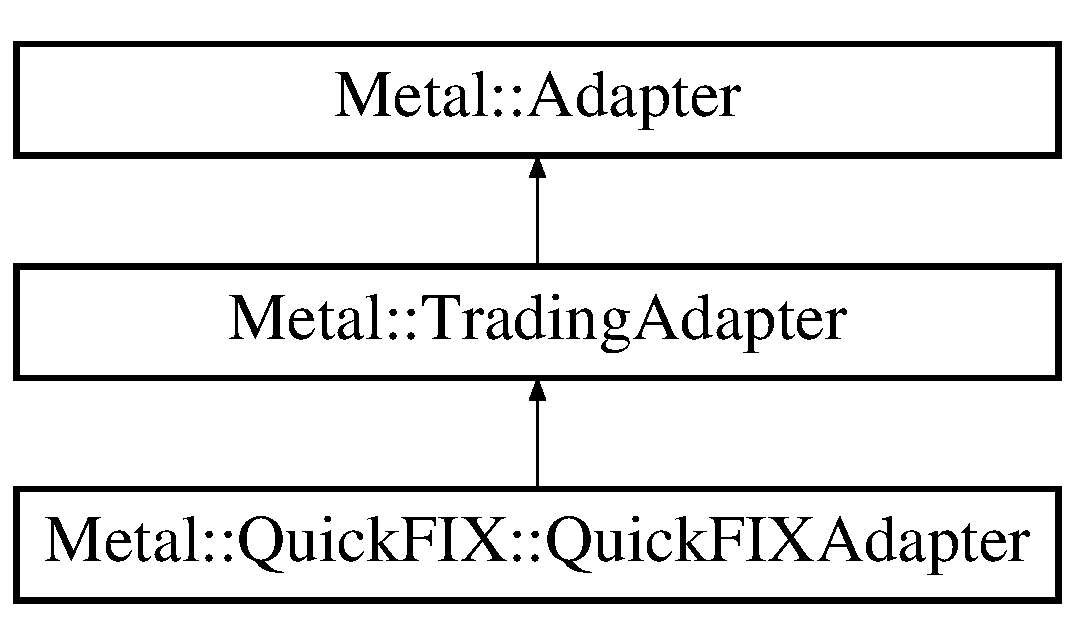
\includegraphics[height=3.000000cm]{classMetal_1_1QuickFIX_1_1QuickFIXAdapter}
\end{center}
\end{figure}
\subsection*{Public Member Functions}
\begin{DoxyCompactItemize}
\item 
\hyperlink{classMetal_1_1QuickFIX_1_1QuickFIXAdapter_ac437c5ed10c4b0ed06a49b31d194be70}{Quick\+F\+I\+X\+Adapter} ()
\item 
void \hyperlink{classMetal_1_1QuickFIX_1_1QuickFIXAdapter_ae53ab5057d4e2003a486ddc5761935a1}{send\+New\+Order} (const \hyperlink{classMetal_1_1NewOrderSingle}{New\+Order\+Single} \&nos)
\item 
virtual void \hyperlink{classMetal_1_1QuickFIX_1_1QuickFIXAdapter_acf1ae68d29b8a22c7252891665d218a8}{on\+Message} (const \hyperlink{namespaceMetal_af4294c176f6aecf9f75e9b106b117aa1}{Execution\+Report} \&er)
\item 
void \hyperlink{classMetal_1_1QuickFIX_1_1QuickFIXAdapter_a20f5db6305b3f479e12553f021765d60}{start} ()
\item 
void \hyperlink{classMetal_1_1QuickFIX_1_1QuickFIXAdapter_af0e438d5d64fa8a0aa3024b5a995f885}{stop} ()
\item 
virtual void \hyperlink{classMetal_1_1QuickFIX_1_1QuickFIXAdapter_ade65590a3da99272d88059e8f031b4d4}{encode\+Logon} (\hyperlink{classMetal_1_1Message}{Message} \&msg)
\item 
virtual void \hyperlink{classMetal_1_1QuickFIX_1_1QuickFIXAdapter_afa4aac6757cb58c2723eda4043156a4a}{encode\+Heart\+Beat} (\hyperlink{classMetal_1_1Message}{Message} \&msg)
\item 
virtual \hyperlink{classMetal_1_1QuickFIX_1_1QuickFIXAdapter_a3023c5d511ae87ee7a1cf73897fd09aa}{$\sim$\+Quick\+F\+I\+X\+Adapter} ()
\end{DoxyCompactItemize}
\subsection*{Static Public Attributes}
\begin{DoxyCompactItemize}
\item 
static const std\+::string \hyperlink{classMetal_1_1QuickFIX_1_1QuickFIXAdapter_aad5f72f920f26469fa0192dcbdb3a59a}{N\+A\+M\+E} = \char`\"{}Quick\+F\+I\+X\char`\"{}
\item 
static const std\+::string \hyperlink{classMetal_1_1QuickFIX_1_1QuickFIXAdapter_aa8a9ed777bdbc2c9a138fa35741da77a}{U\+U\+I\+D} = \char`\"{}e32cd5d0-\/4564-\/11e4-\/916c-\/0800200c9a66\char`\"{}
\end{DoxyCompactItemize}
\subsection*{Protected Member Functions}
\begin{DoxyCompactItemize}
\item 
int \hyperlink{classMetal_1_1QuickFIX_1_1QuickFIXAdapter_a0598785e8408706cde97d532090d3fcb}{process\+Data} (const char $\ast$data, int length)
\item 
void \hyperlink{classMetal_1_1QuickFIX_1_1QuickFIXAdapter_a6bb8af5a8dd9c4ad157bce0e8ef35ef1}{send\+Heart\+Beat} ()
\item 
void \hyperlink{classMetal_1_1QuickFIX_1_1QuickFIXAdapter_a3f9dba36bbaa3d8db8af62ac07a9fff5}{send\+Logon} ()
\end{DoxyCompactItemize}
\subsection*{Additional Inherited Members}


\subsection{Constructor \& Destructor Documentation}
\hypertarget{classMetal_1_1QuickFIX_1_1QuickFIXAdapter_ac437c5ed10c4b0ed06a49b31d194be70}{}\index{Metal\+::\+Quick\+F\+I\+X\+::\+Quick\+F\+I\+X\+Adapter@{Metal\+::\+Quick\+F\+I\+X\+::\+Quick\+F\+I\+X\+Adapter}!Quick\+F\+I\+X\+Adapter@{Quick\+F\+I\+X\+Adapter}}
\index{Quick\+F\+I\+X\+Adapter@{Quick\+F\+I\+X\+Adapter}!Metal\+::\+Quick\+F\+I\+X\+::\+Quick\+F\+I\+X\+Adapter@{Metal\+::\+Quick\+F\+I\+X\+::\+Quick\+F\+I\+X\+Adapter}}
\subsubsection[{Quick\+F\+I\+X\+Adapter}]{\setlength{\rightskip}{0pt plus 5cm}Metal\+::\+Quick\+F\+I\+X\+::\+Quick\+F\+I\+X\+Adapter\+::\+Quick\+F\+I\+X\+Adapter (
\begin{DoxyParamCaption}
{}
\end{DoxyParamCaption}
)}\label{classMetal_1_1QuickFIX_1_1QuickFIXAdapter_ac437c5ed10c4b0ed06a49b31d194be70}
Default Constructor \hypertarget{classMetal_1_1QuickFIX_1_1QuickFIXAdapter_a3023c5d511ae87ee7a1cf73897fd09aa}{}\index{Metal\+::\+Quick\+F\+I\+X\+::\+Quick\+F\+I\+X\+Adapter@{Metal\+::\+Quick\+F\+I\+X\+::\+Quick\+F\+I\+X\+Adapter}!````~Quick\+F\+I\+X\+Adapter@{$\sim$\+Quick\+F\+I\+X\+Adapter}}
\index{````~Quick\+F\+I\+X\+Adapter@{$\sim$\+Quick\+F\+I\+X\+Adapter}!Metal\+::\+Quick\+F\+I\+X\+::\+Quick\+F\+I\+X\+Adapter@{Metal\+::\+Quick\+F\+I\+X\+::\+Quick\+F\+I\+X\+Adapter}}
\subsubsection[{$\sim$\+Quick\+F\+I\+X\+Adapter}]{\setlength{\rightskip}{0pt plus 5cm}virtual Metal\+::\+Quick\+F\+I\+X\+::\+Quick\+F\+I\+X\+Adapter\+::$\sim$\+Quick\+F\+I\+X\+Adapter (
\begin{DoxyParamCaption}
{}
\end{DoxyParamCaption}
)\hspace{0.3cm}{\ttfamily [inline]}, {\ttfamily [virtual]}}\label{classMetal_1_1QuickFIX_1_1QuickFIXAdapter_a3023c5d511ae87ee7a1cf73897fd09aa}


\subsection{Member Function Documentation}
\hypertarget{classMetal_1_1QuickFIX_1_1QuickFIXAdapter_afa4aac6757cb58c2723eda4043156a4a}{}\index{Metal\+::\+Quick\+F\+I\+X\+::\+Quick\+F\+I\+X\+Adapter@{Metal\+::\+Quick\+F\+I\+X\+::\+Quick\+F\+I\+X\+Adapter}!encode\+Heart\+Beat@{encode\+Heart\+Beat}}
\index{encode\+Heart\+Beat@{encode\+Heart\+Beat}!Metal\+::\+Quick\+F\+I\+X\+::\+Quick\+F\+I\+X\+Adapter@{Metal\+::\+Quick\+F\+I\+X\+::\+Quick\+F\+I\+X\+Adapter}}
\subsubsection[{encode\+Heart\+Beat}]{\setlength{\rightskip}{0pt plus 5cm}virtual void Metal\+::\+Quick\+F\+I\+X\+::\+Quick\+F\+I\+X\+Adapter\+::encode\+Heart\+Beat (
\begin{DoxyParamCaption}
\item[{{\bf Message} \&}]{msg}
\end{DoxyParamCaption}
)\hspace{0.3cm}{\ttfamily [inline]}, {\ttfamily [virtual]}}\label{classMetal_1_1QuickFIX_1_1QuickFIXAdapter_afa4aac6757cb58c2723eda4043156a4a}
\hypertarget{classMetal_1_1QuickFIX_1_1QuickFIXAdapter_ade65590a3da99272d88059e8f031b4d4}{}\index{Metal\+::\+Quick\+F\+I\+X\+::\+Quick\+F\+I\+X\+Adapter@{Metal\+::\+Quick\+F\+I\+X\+::\+Quick\+F\+I\+X\+Adapter}!encode\+Logon@{encode\+Logon}}
\index{encode\+Logon@{encode\+Logon}!Metal\+::\+Quick\+F\+I\+X\+::\+Quick\+F\+I\+X\+Adapter@{Metal\+::\+Quick\+F\+I\+X\+::\+Quick\+F\+I\+X\+Adapter}}
\subsubsection[{encode\+Logon}]{\setlength{\rightskip}{0pt plus 5cm}virtual void Metal\+::\+Quick\+F\+I\+X\+::\+Quick\+F\+I\+X\+Adapter\+::encode\+Logon (
\begin{DoxyParamCaption}
\item[{{\bf Message} \&}]{msg}
\end{DoxyParamCaption}
)\hspace{0.3cm}{\ttfamily [inline]}, {\ttfamily [virtual]}}\label{classMetal_1_1QuickFIX_1_1QuickFIXAdapter_ade65590a3da99272d88059e8f031b4d4}
We don't need to provide \hyperlink{classMetal_1_1Logon}{Logon} Encoding because \hyperlink{namespaceMetal_1_1QuickFIX}{Quick\+F\+I\+X} provides its own session management \hypertarget{classMetal_1_1QuickFIX_1_1QuickFIXAdapter_acf1ae68d29b8a22c7252891665d218a8}{}\index{Metal\+::\+Quick\+F\+I\+X\+::\+Quick\+F\+I\+X\+Adapter@{Metal\+::\+Quick\+F\+I\+X\+::\+Quick\+F\+I\+X\+Adapter}!on\+Message@{on\+Message}}
\index{on\+Message@{on\+Message}!Metal\+::\+Quick\+F\+I\+X\+::\+Quick\+F\+I\+X\+Adapter@{Metal\+::\+Quick\+F\+I\+X\+::\+Quick\+F\+I\+X\+Adapter}}
\subsubsection[{on\+Message}]{\setlength{\rightskip}{0pt plus 5cm}void Metal\+::\+Quick\+F\+I\+X\+::\+Quick\+F\+I\+X\+Adapter\+::on\+Message (
\begin{DoxyParamCaption}
\item[{const {\bf Execution\+Report} \&}]{er}
\end{DoxyParamCaption}
)\hspace{0.3cm}{\ttfamily [virtual]}}\label{classMetal_1_1QuickFIX_1_1QuickFIXAdapter_acf1ae68d29b8a22c7252891665d218a8}
This method will invoked upon receiving a normalized execution report~\newline
 Subclasses should override this method to capture execution reports in generic format~\newline
 
\begin{DoxyParams}{Parameters}
{\em Execution\+Report} & incomming execution report \\
\hline
\end{DoxyParams}


Reimplemented from \hyperlink{classMetal_1_1TradingAdapter_a44332505b213c0428d901ef6a530efff}{Metal\+::\+Trading\+Adapter}.

\hypertarget{classMetal_1_1QuickFIX_1_1QuickFIXAdapter_a0598785e8408706cde97d532090d3fcb}{}\index{Metal\+::\+Quick\+F\+I\+X\+::\+Quick\+F\+I\+X\+Adapter@{Metal\+::\+Quick\+F\+I\+X\+::\+Quick\+F\+I\+X\+Adapter}!process\+Data@{process\+Data}}
\index{process\+Data@{process\+Data}!Metal\+::\+Quick\+F\+I\+X\+::\+Quick\+F\+I\+X\+Adapter@{Metal\+::\+Quick\+F\+I\+X\+::\+Quick\+F\+I\+X\+Adapter}}
\subsubsection[{process\+Data}]{\setlength{\rightskip}{0pt plus 5cm}int Metal\+::\+Quick\+F\+I\+X\+::\+Quick\+F\+I\+X\+Adapter\+::process\+Data (
\begin{DoxyParamCaption}
\item[{const char $\ast$}]{data, }
\item[{int}]{length}
\end{DoxyParamCaption}
)\hspace{0.3cm}{\ttfamily [inline]}, {\ttfamily [protected]}, {\ttfamily [virtual]}}\label{classMetal_1_1QuickFIX_1_1QuickFIXAdapter_a0598785e8408706cde97d532090d3fcb}
We don't implement a real data processor because we are leveraging \hyperlink{namespaceMetal_1_1QuickFIX}{Quick\+F\+I\+X} parsing ability 

Implements \hyperlink{classMetal_1_1Adapter_a195072772568dc0fd7a859ed2c99d5c7}{Metal\+::\+Adapter}.

\hypertarget{classMetal_1_1QuickFIX_1_1QuickFIXAdapter_a6bb8af5a8dd9c4ad157bce0e8ef35ef1}{}\index{Metal\+::\+Quick\+F\+I\+X\+::\+Quick\+F\+I\+X\+Adapter@{Metal\+::\+Quick\+F\+I\+X\+::\+Quick\+F\+I\+X\+Adapter}!send\+Heart\+Beat@{send\+Heart\+Beat}}
\index{send\+Heart\+Beat@{send\+Heart\+Beat}!Metal\+::\+Quick\+F\+I\+X\+::\+Quick\+F\+I\+X\+Adapter@{Metal\+::\+Quick\+F\+I\+X\+::\+Quick\+F\+I\+X\+Adapter}}
\subsubsection[{send\+Heart\+Beat}]{\setlength{\rightskip}{0pt plus 5cm}void Metal\+::\+Quick\+F\+I\+X\+::\+Quick\+F\+I\+X\+Adapter\+::send\+Heart\+Beat (
\begin{DoxyParamCaption}
{}
\end{DoxyParamCaption}
)\hspace{0.3cm}{\ttfamily [inline]}, {\ttfamily [protected]}, {\ttfamily [virtual]}}\label{classMetal_1_1QuickFIX_1_1QuickFIXAdapter_a6bb8af5a8dd9c4ad157bce0e8ef35ef1}
Formats and sends a Heart Beat message 

Implements \hyperlink{classMetal_1_1TradingAdapter_a39caec739aaad9593ba1b93b8e130385}{Metal\+::\+Trading\+Adapter}.

\hypertarget{classMetal_1_1QuickFIX_1_1QuickFIXAdapter_a3f9dba36bbaa3d8db8af62ac07a9fff5}{}\index{Metal\+::\+Quick\+F\+I\+X\+::\+Quick\+F\+I\+X\+Adapter@{Metal\+::\+Quick\+F\+I\+X\+::\+Quick\+F\+I\+X\+Adapter}!send\+Logon@{send\+Logon}}
\index{send\+Logon@{send\+Logon}!Metal\+::\+Quick\+F\+I\+X\+::\+Quick\+F\+I\+X\+Adapter@{Metal\+::\+Quick\+F\+I\+X\+::\+Quick\+F\+I\+X\+Adapter}}
\subsubsection[{send\+Logon}]{\setlength{\rightskip}{0pt plus 5cm}void Metal\+::\+Quick\+F\+I\+X\+::\+Quick\+F\+I\+X\+Adapter\+::send\+Logon (
\begin{DoxyParamCaption}
{}
\end{DoxyParamCaption}
)\hspace{0.3cm}{\ttfamily [inline]}, {\ttfamily [protected]}, {\ttfamily [virtual]}}\label{classMetal_1_1QuickFIX_1_1QuickFIXAdapter_a3f9dba36bbaa3d8db8af62ac07a9fff5}
Sends a logon message to initiate the session 

Implements \hyperlink{classMetal_1_1TradingAdapter_a39562015df3e7202a5e8f932b8bde43e}{Metal\+::\+Trading\+Adapter}.

\hypertarget{classMetal_1_1QuickFIX_1_1QuickFIXAdapter_ae53ab5057d4e2003a486ddc5761935a1}{}\index{Metal\+::\+Quick\+F\+I\+X\+::\+Quick\+F\+I\+X\+Adapter@{Metal\+::\+Quick\+F\+I\+X\+::\+Quick\+F\+I\+X\+Adapter}!send\+New\+Order@{send\+New\+Order}}
\index{send\+New\+Order@{send\+New\+Order}!Metal\+::\+Quick\+F\+I\+X\+::\+Quick\+F\+I\+X\+Adapter@{Metal\+::\+Quick\+F\+I\+X\+::\+Quick\+F\+I\+X\+Adapter}}
\subsubsection[{send\+New\+Order}]{\setlength{\rightskip}{0pt plus 5cm}void Metal\+::\+Quick\+F\+I\+X\+::\+Quick\+F\+I\+X\+Adapter\+::send\+New\+Order (
\begin{DoxyParamCaption}
\item[{const {\bf New\+Order\+Single} \&}]{nos}
\end{DoxyParamCaption}
)\hspace{0.3cm}{\ttfamily [virtual]}}\label{classMetal_1_1QuickFIX_1_1QuickFIXAdapter_ae53ab5057d4e2003a486ddc5761935a1}
We override this method to leverage \hyperlink{namespaceMetal_1_1QuickFIX}{Quick\+F\+I\+X} sending capacity

Send normalized New Order 

Implements \hyperlink{classMetal_1_1TradingAdapter_abccc3fdb238887112e1a0820a70f0fce}{Metal\+::\+Trading\+Adapter}.

\hypertarget{classMetal_1_1QuickFIX_1_1QuickFIXAdapter_a20f5db6305b3f479e12553f021765d60}{}\index{Metal\+::\+Quick\+F\+I\+X\+::\+Quick\+F\+I\+X\+Adapter@{Metal\+::\+Quick\+F\+I\+X\+::\+Quick\+F\+I\+X\+Adapter}!start@{start}}
\index{start@{start}!Metal\+::\+Quick\+F\+I\+X\+::\+Quick\+F\+I\+X\+Adapter@{Metal\+::\+Quick\+F\+I\+X\+::\+Quick\+F\+I\+X\+Adapter}}
\subsubsection[{start}]{\setlength{\rightskip}{0pt plus 5cm}void Metal\+::\+Quick\+F\+I\+X\+::\+Quick\+F\+I\+X\+Adapter\+::start (
\begin{DoxyParamCaption}
{}
\end{DoxyParamCaption}
)\hspace{0.3cm}{\ttfamily [virtual]}}\label{classMetal_1_1QuickFIX_1_1QuickFIXAdapter_a20f5db6305b3f479e12553f021765d60}
We are overidding start to prevent \hyperlink{classMetal_1_1Adapter}{Adapter} processing of session life cycle 

Reimplemented from \hyperlink{classMetal_1_1Adapter_adeed43dfa9e2d18bd66dd2f806b1e182}{Metal\+::\+Adapter}.

\hypertarget{classMetal_1_1QuickFIX_1_1QuickFIXAdapter_af0e438d5d64fa8a0aa3024b5a995f885}{}\index{Metal\+::\+Quick\+F\+I\+X\+::\+Quick\+F\+I\+X\+Adapter@{Metal\+::\+Quick\+F\+I\+X\+::\+Quick\+F\+I\+X\+Adapter}!stop@{stop}}
\index{stop@{stop}!Metal\+::\+Quick\+F\+I\+X\+::\+Quick\+F\+I\+X\+Adapter@{Metal\+::\+Quick\+F\+I\+X\+::\+Quick\+F\+I\+X\+Adapter}}
\subsubsection[{stop}]{\setlength{\rightskip}{0pt plus 5cm}void Metal\+::\+Quick\+F\+I\+X\+::\+Quick\+F\+I\+X\+Adapter\+::stop (
\begin{DoxyParamCaption}
{}
\end{DoxyParamCaption}
)}\label{classMetal_1_1QuickFIX_1_1QuickFIXAdapter_af0e438d5d64fa8a0aa3024b5a995f885}


\subsection{Member Data Documentation}
\hypertarget{classMetal_1_1QuickFIX_1_1QuickFIXAdapter_aad5f72f920f26469fa0192dcbdb3a59a}{}\index{Metal\+::\+Quick\+F\+I\+X\+::\+Quick\+F\+I\+X\+Adapter@{Metal\+::\+Quick\+F\+I\+X\+::\+Quick\+F\+I\+X\+Adapter}!N\+A\+M\+E@{N\+A\+M\+E}}
\index{N\+A\+M\+E@{N\+A\+M\+E}!Metal\+::\+Quick\+F\+I\+X\+::\+Quick\+F\+I\+X\+Adapter@{Metal\+::\+Quick\+F\+I\+X\+::\+Quick\+F\+I\+X\+Adapter}}
\subsubsection[{N\+A\+M\+E}]{\setlength{\rightskip}{0pt plus 5cm}const std\+::string Metal\+::\+Quick\+F\+I\+X\+::\+Quick\+F\+I\+X\+Adapter\+::\+N\+A\+M\+E = \char`\"{}Quick\+F\+I\+X\char`\"{}\hspace{0.3cm}{\ttfamily [static]}}\label{classMetal_1_1QuickFIX_1_1QuickFIXAdapter_aad5f72f920f26469fa0192dcbdb3a59a}
\hypertarget{classMetal_1_1QuickFIX_1_1QuickFIXAdapter_aa8a9ed777bdbc2c9a138fa35741da77a}{}\index{Metal\+::\+Quick\+F\+I\+X\+::\+Quick\+F\+I\+X\+Adapter@{Metal\+::\+Quick\+F\+I\+X\+::\+Quick\+F\+I\+X\+Adapter}!U\+U\+I\+D@{U\+U\+I\+D}}
\index{U\+U\+I\+D@{U\+U\+I\+D}!Metal\+::\+Quick\+F\+I\+X\+::\+Quick\+F\+I\+X\+Adapter@{Metal\+::\+Quick\+F\+I\+X\+::\+Quick\+F\+I\+X\+Adapter}}
\subsubsection[{U\+U\+I\+D}]{\setlength{\rightskip}{0pt plus 5cm}const std\+::string Metal\+::\+Quick\+F\+I\+X\+::\+Quick\+F\+I\+X\+Adapter\+::\+U\+U\+I\+D = \char`\"{}e32cd5d0-\/4564-\/11e4-\/916c-\/0800200c9a66\char`\"{}\hspace{0.3cm}{\ttfamily [static]}}\label{classMetal_1_1QuickFIX_1_1QuickFIXAdapter_aa8a9ed777bdbc2c9a138fa35741da77a}


The documentation for this class was generated from the following files\+:\begin{DoxyCompactItemize}
\item 
/home/jc/metal/github/src/adapters/\+Quick\+F\+I\+X\+Adapter/\hyperlink{QuickFIXAdapter_8h}{Quick\+F\+I\+X\+Adapter.\+h}\item 
/home/jc/metal/github/src/adapters/\+Quick\+F\+I\+X\+Adapter/\hyperlink{QuickFIXAdapter_8cpp}{Quick\+F\+I\+X\+Adapter.\+cpp}\end{DoxyCompactItemize}

\hypertarget{classMetal_1_1QuickFIXMessageMapper}{}\section{Metal\+:\+:Quick\+F\+I\+X\+Message\+Mapper Class Reference}
\label{classMetal_1_1QuickFIXMessageMapper}\index{Metal\+::\+Quick\+F\+I\+X\+Message\+Mapper@{Metal\+::\+Quick\+F\+I\+X\+Message\+Mapper}}
Inheritance diagram for Metal\+:\+:Quick\+F\+I\+X\+Message\+Mapper\+:\begin{figure}[H]
\begin{center}
\leavevmode
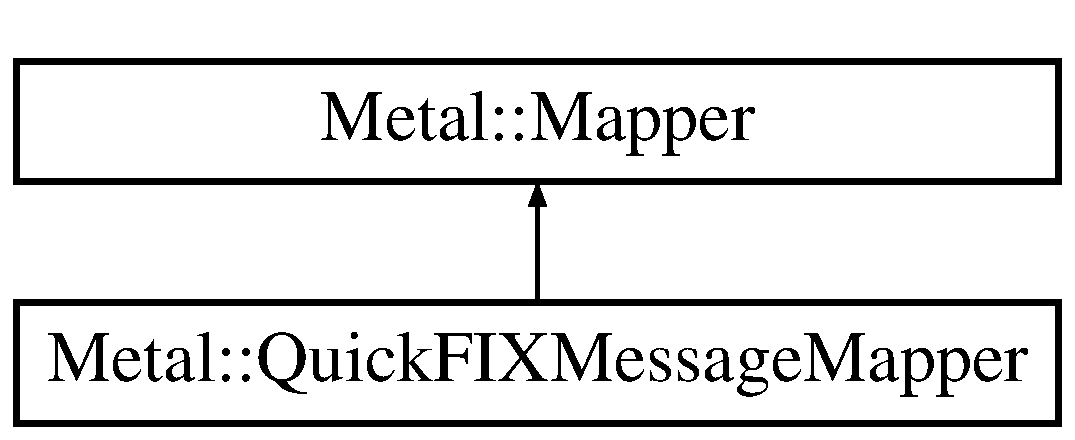
\includegraphics[height=2.000000cm]{classMetal_1_1QuickFIXMessageMapper}
\end{center}
\end{figure}
\subsection*{Static Public Member Functions}
\begin{DoxyCompactItemize}
\item 
static void \hyperlink{classMetal_1_1QuickFIXMessageMapper_ad42b0f6ed92b6e777e3716de55b20f21}{map} (const F\+I\+X44\+::\+New\+Order\+Single \&, \hyperlink{classMetal_1_1NewOrderSingle}{New\+Order\+Single} \&)
\item 
static void \hyperlink{classMetal_1_1QuickFIXMessageMapper_a98184463c76af4e0a21e8dfbd4b61af4}{map} (const F\+I\+X44\+::\+Execution\+Report \&, Execution\+Report \&)
\item 
static void \hyperlink{classMetal_1_1QuickFIXMessageMapper_ad5c9c32bc745db35e7d2a472cb204514}{map} (const \hyperlink{classMetal_1_1NewOrderSingle}{New\+Order\+Single} \&, F\+I\+X\+::\+Message \&)
\item 
static void \hyperlink{classMetal_1_1QuickFIXMessageMapper_ab7692db7b3f7b616acd7c6e9fc024d2c}{map} (const \hyperlink{classMetal_1_1OrderCancelRequest}{Order\+Cancel\+Request} \&, F\+I\+X\+::\+Message \&)
\end{DoxyCompactItemize}


\subsection{Member Function Documentation}
\hypertarget{classMetal_1_1QuickFIXMessageMapper_ad42b0f6ed92b6e777e3716de55b20f21}{}\index{Metal\+::\+Quick\+F\+I\+X\+Message\+Mapper@{Metal\+::\+Quick\+F\+I\+X\+Message\+Mapper}!map@{map}}
\index{map@{map}!Metal\+::\+Quick\+F\+I\+X\+Message\+Mapper@{Metal\+::\+Quick\+F\+I\+X\+Message\+Mapper}}
\subsubsection[{map}]{\setlength{\rightskip}{0pt plus 5cm}void Metal\+::\+Quick\+F\+I\+X\+Message\+Mapper\+::map (
\begin{DoxyParamCaption}
\item[{const F\+I\+X44\+::\+New\+Order\+Single \&}]{message, }
\item[{{\bf New\+Order\+Single} \&}]{nos}
\end{DoxyParamCaption}
)\hspace{0.3cm}{\ttfamily [static]}}\label{classMetal_1_1QuickFIXMessageMapper_ad42b0f6ed92b6e777e3716de55b20f21}
Translate F\+I\+X \hyperlink{classMetal_1_1NewOrderSingle}{New\+Order\+Single} into Metal representation \hypertarget{classMetal_1_1QuickFIXMessageMapper_a98184463c76af4e0a21e8dfbd4b61af4}{}\index{Metal\+::\+Quick\+F\+I\+X\+Message\+Mapper@{Metal\+::\+Quick\+F\+I\+X\+Message\+Mapper}!map@{map}}
\index{map@{map}!Metal\+::\+Quick\+F\+I\+X\+Message\+Mapper@{Metal\+::\+Quick\+F\+I\+X\+Message\+Mapper}}
\subsubsection[{map}]{\setlength{\rightskip}{0pt plus 5cm}void Metal\+::\+Quick\+F\+I\+X\+Message\+Mapper\+::map (
\begin{DoxyParamCaption}
\item[{const F\+I\+X44\+::\+Execution\+Report \&}]{message, }
\item[{Execution\+Report \&}]{er}
\end{DoxyParamCaption}
)\hspace{0.3cm}{\ttfamily [static]}}\label{classMetal_1_1QuickFIXMessageMapper_a98184463c76af4e0a21e8dfbd4b61af4}
Execution Report F\+I\+X -\/$>$ Me\+T\+A\+L \hypertarget{classMetal_1_1QuickFIXMessageMapper_ad5c9c32bc745db35e7d2a472cb204514}{}\index{Metal\+::\+Quick\+F\+I\+X\+Message\+Mapper@{Metal\+::\+Quick\+F\+I\+X\+Message\+Mapper}!map@{map}}
\index{map@{map}!Metal\+::\+Quick\+F\+I\+X\+Message\+Mapper@{Metal\+::\+Quick\+F\+I\+X\+Message\+Mapper}}
\subsubsection[{map}]{\setlength{\rightskip}{0pt plus 5cm}void Metal\+::\+Quick\+F\+I\+X\+Message\+Mapper\+::map (
\begin{DoxyParamCaption}
\item[{const {\bf New\+Order\+Single} \&}]{nos, }
\item[{F\+I\+X\+::\+Message \&}]{message}
\end{DoxyParamCaption}
)\hspace{0.3cm}{\ttfamily [static]}}\label{classMetal_1_1QuickFIXMessageMapper_ad5c9c32bc745db35e7d2a472cb204514}
Me\+T\+A\+L to F\+I\+X44 transformation for \hyperlink{classMetal_1_1NewOrderSingle}{New\+Order\+Single}

\hyperlink{classMetal_1_1NewOrderSingle}{New\+Order\+Single} Me\+T\+A\+L -\/$>$ F\+I\+X44 \hypertarget{classMetal_1_1QuickFIXMessageMapper_ab7692db7b3f7b616acd7c6e9fc024d2c}{}\index{Metal\+::\+Quick\+F\+I\+X\+Message\+Mapper@{Metal\+::\+Quick\+F\+I\+X\+Message\+Mapper}!map@{map}}
\index{map@{map}!Metal\+::\+Quick\+F\+I\+X\+Message\+Mapper@{Metal\+::\+Quick\+F\+I\+X\+Message\+Mapper}}
\subsubsection[{map}]{\setlength{\rightskip}{0pt plus 5cm}void Metal\+::\+Quick\+F\+I\+X\+Message\+Mapper\+::map (
\begin{DoxyParamCaption}
\item[{const {\bf Order\+Cancel\+Request} \&}]{ocr, }
\item[{F\+I\+X\+::\+Message \&}]{message}
\end{DoxyParamCaption}
)\hspace{0.3cm}{\ttfamily [static]}}\label{classMetal_1_1QuickFIXMessageMapper_ab7692db7b3f7b616acd7c6e9fc024d2c}
Me\+T\+A\+L to F\+I\+X44 transformation for \hyperlink{classMetal_1_1OrderCancelRequest}{Order\+Cancel\+Request} 

The documentation for this class was generated from the following files\+:\begin{DoxyCompactItemize}
\item 
/home/jc/metal/src/metal/adapters/\+Quick\+F\+I\+X\+Adapter/Quick\+F\+I\+X\+Message\+Mapper.\+h\item 
/home/jc/metal/src/metal/adapters/\+Quick\+F\+I\+X\+Adapter/Quick\+F\+I\+X\+Message\+Mapper.\+cpp\end{DoxyCompactItemize}

\hypertarget{classMetal_1_1SendMessageException}{}\section{Metal\+:\+:Send\+Message\+Exception Class Reference}
\label{classMetal_1_1SendMessageException}\index{Metal\+::\+Send\+Message\+Exception@{Metal\+::\+Send\+Message\+Exception}}
Inheritance diagram for Metal\+:\+:Send\+Message\+Exception\+:\begin{figure}[H]
\begin{center}
\leavevmode
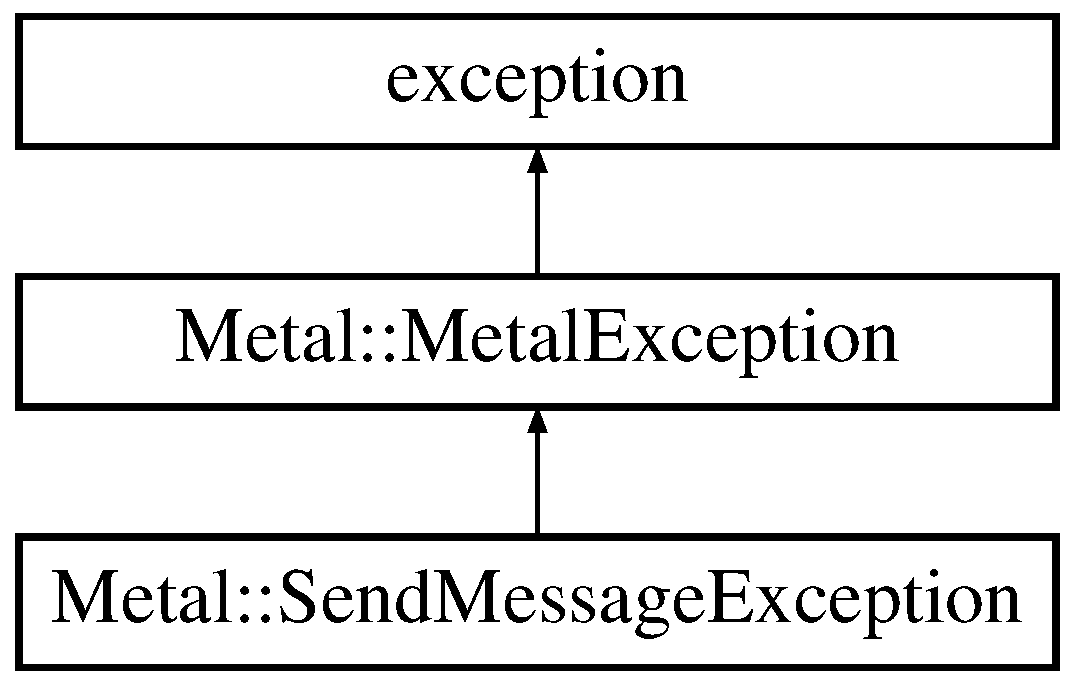
\includegraphics[height=3.000000cm]{classMetal_1_1SendMessageException}
\end{center}
\end{figure}
\subsection*{Public Member Functions}
\begin{DoxyCompactItemize}
\item 
\hypertarget{classMetal_1_1SendMessageException_a4aeb690808ab3639bbd837b7c57cc419}{}{\bfseries Send\+Message\+Exception} (const std\+::string \&message)\label{classMetal_1_1SendMessageException_a4aeb690808ab3639bbd837b7c57cc419}

\end{DoxyCompactItemize}


The documentation for this class was generated from the following file\+:\begin{DoxyCompactItemize}
\item 
/home/jc/metal/src/metal/Metal\+Exceptions.\+h\end{DoxyCompactItemize}

\hypertarget{classMetal_1_1TradingAdapter}{}\section{Metal\+:\+:Trading\+Adapter Class Reference}
\label{classMetal_1_1TradingAdapter}\index{Metal\+::\+Trading\+Adapter@{Metal\+::\+Trading\+Adapter}}
Inheritance diagram for Metal\+:\+:Trading\+Adapter\+:\begin{figure}[H]
\begin{center}
\leavevmode
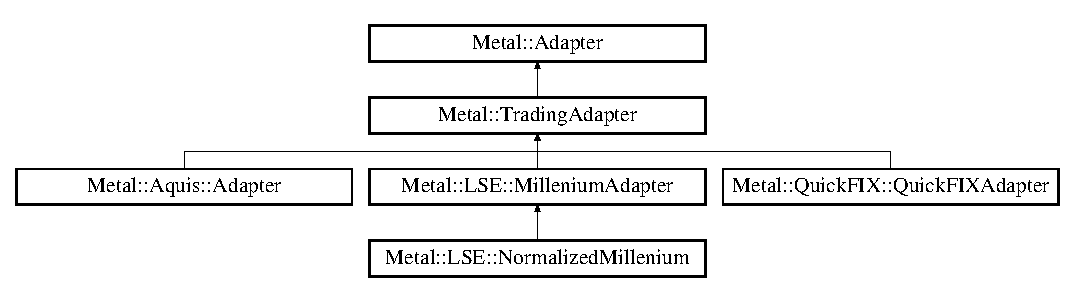
\includegraphics[height=3.000000cm]{classMetal_1_1TradingAdapter}
\end{center}
\end{figure}
\subsection*{Public Member Functions}
\begin{DoxyCompactItemize}
\item 
\hyperlink{classMetal_1_1TradingAdapter_a472ad74753a0bd77a3e78c1f7f8d0398}{Trading\+Adapter} (const std\+::string \&name, const std\+::string \&uuid)
\item 
void \hyperlink{classMetal_1_1TradingAdapter_ae0b309ccc7e9ec5dfe262d071dde4c17}{set\+Remote\+Host} (const std\+::string \&host\+Name, unsigned int port\+Number)
\item 
void \hyperlink{classMetal_1_1TradingAdapter_a1ba0cd89d6475faf9da358140660e886}{start} ()
\item 
void \hyperlink{classMetal_1_1TradingAdapter_aa5e283e9e0a339c738cfba37fed3c7ff}{stop} ()
\item 
void \hyperlink{classMetal_1_1TradingAdapter_ac99cc99c695715fc396756441e68abc0}{send} (\hyperlink{classMetal_1_1Message}{Message} \&msg)
\item 
virtual void \hyperlink{classMetal_1_1TradingAdapter_a2ecc8f1c8fe8a8d29625d142f473f1c3}{send} (const \hyperlink{classMetal_1_1NewOrderSingle}{New\+Order\+Single} \&)=0
\item 
virtual void \hyperlink{classMetal_1_1TradingAdapter_a39562015df3e7202a5e8f932b8bde43e}{send\+Logon} ()=0
\item 
virtual void \hyperlink{classMetal_1_1TradingAdapter_af0015d51815dedb1bc78258b3030d751}{recv} (const Execution\+Report \&er)=0
\item 
virtual void \hyperlink{classMetal_1_1TradingAdapter_a10208ab030e4b3a9db4dc71206a1812e}{on\+Physical\+Connection} ()
\item 
virtual void \hyperlink{classMetal_1_1TradingAdapter_a161ad3db17091807d091d1b236de0105}{benchmark} (const std\+::vector$<$ \hyperlink{classMetal_1_1NewOrderSingle}{New\+Order\+Single} $>$ \&list, std\+::chrono\+::milliseconds \&mapping\+Duration, std\+::chrono\+::milliseconds \&encoding\+Duration)=0
\item 
virtual void \hyperlink{classMetal_1_1TradingAdapter_ae0513f6865414f61a41a8f62bafb0187}{benchmark} (const std\+::vector$<$ \hyperlink{classMetal_1_1OrderCancelRequest}{Order\+Cancel\+Request} $>$ \&list, std\+::chrono\+::milliseconds \&mapping\+Duration, std\+::chrono\+::milliseconds \&encoding\+Duration)=0
\end{DoxyCompactItemize}
\subsection*{Protected Member Functions}
\begin{DoxyCompactItemize}
\item 
void \hyperlink{classMetal_1_1TradingAdapter_a51851f504678002634259b8fd5b22d3e}{close\+Socket} (int delay=0)
\end{DoxyCompactItemize}
\subsection*{Protected Attributes}
\begin{DoxyCompactItemize}
\item 
\hypertarget{classMetal_1_1TradingAdapter_a0948ce848a4bd3f4d48019dde792eb5d}{}std\+::string {\bfseries remote\+Host}\label{classMetal_1_1TradingAdapter_a0948ce848a4bd3f4d48019dde792eb5d}

\item 
\hypertarget{classMetal_1_1TradingAdapter_ac657baf65b2e469f6fa9b641ca50cc21}{}unsigned int {\bfseries remote\+Port}\label{classMetal_1_1TradingAdapter_ac657baf65b2e469f6fa9b641ca50cc21}

\item 
\hypertarget{classMetal_1_1TradingAdapter_a1a742b88c94b305071035985437f49c2}{}N\+L\+::\+Socket $\ast$ {\bfseries socket}\label{classMetal_1_1TradingAdapter_a1a742b88c94b305071035985437f49c2}

\end{DoxyCompactItemize}


\subsection{Constructor \& Destructor Documentation}
\hypertarget{classMetal_1_1TradingAdapter_a472ad74753a0bd77a3e78c1f7f8d0398}{}\index{Metal\+::\+Trading\+Adapter@{Metal\+::\+Trading\+Adapter}!Trading\+Adapter@{Trading\+Adapter}}
\index{Trading\+Adapter@{Trading\+Adapter}!Metal\+::\+Trading\+Adapter@{Metal\+::\+Trading\+Adapter}}
\subsubsection[{Trading\+Adapter}]{\setlength{\rightskip}{0pt plus 5cm}Metal\+::\+Trading\+Adapter\+::\+Trading\+Adapter (
\begin{DoxyParamCaption}
\item[{const std\+::string \&}]{name, }
\item[{const std\+::string \&}]{uuid}
\end{DoxyParamCaption}
)}\label{classMetal_1_1TradingAdapter_a472ad74753a0bd77a3e78c1f7f8d0398}

\begin{DoxyParams}{Parameters}
{\em name} & Whatever should be used to identify this adapter. Subclasses will perform mapping, encoding then write to the active session \\
\hline
\end{DoxyParams}


\subsection{Member Function Documentation}
\hypertarget{classMetal_1_1TradingAdapter_a161ad3db17091807d091d1b236de0105}{}\index{Metal\+::\+Trading\+Adapter@{Metal\+::\+Trading\+Adapter}!benchmark@{benchmark}}
\index{benchmark@{benchmark}!Metal\+::\+Trading\+Adapter@{Metal\+::\+Trading\+Adapter}}
\subsubsection[{benchmark}]{\setlength{\rightskip}{0pt plus 5cm}virtual void Metal\+::\+Trading\+Adapter\+::benchmark (
\begin{DoxyParamCaption}
\item[{const std\+::vector$<$ {\bf New\+Order\+Single} $>$ \&}]{list, }
\item[{std\+::chrono\+::milliseconds \&}]{mapping\+Duration, }
\item[{std\+::chrono\+::milliseconds \&}]{encoding\+Duration}
\end{DoxyParamCaption}
)\hspace{0.3cm}{\ttfamily [pure virtual]}}\label{classMetal_1_1TradingAdapter_a161ad3db17091807d091d1b236de0105}
The purpose is to measure Mapping and Encoding speed for \hyperlink{classMetal_1_1NewOrderSingle}{New\+Order\+Single}~\newline
 Subclasses should make sure to execute both as opposed to just mapping 
\begin{DoxyParams}{Parameters}
{\em list} & A list of \hyperlink{classMetal_1_1NewOrderSingle}{New\+Order\+Single} better if randomly generated \\
\hline
{\em mapping\+Duration} & Time used to map messages \\
\hline
{\em encoding\+Duration} & Time used to encode messages \\
\hline
\end{DoxyParams}


Implemented in \hyperlink{classMetal_1_1QuickFIX_1_1QuickFIXAdapter_ae987b07f906db9fc74d7f7a55eb38efe}{Metal\+::\+Quick\+F\+I\+X\+::\+Quick\+F\+I\+X\+Adapter}.

\hypertarget{classMetal_1_1TradingAdapter_ae0513f6865414f61a41a8f62bafb0187}{}\index{Metal\+::\+Trading\+Adapter@{Metal\+::\+Trading\+Adapter}!benchmark@{benchmark}}
\index{benchmark@{benchmark}!Metal\+::\+Trading\+Adapter@{Metal\+::\+Trading\+Adapter}}
\subsubsection[{benchmark}]{\setlength{\rightskip}{0pt plus 5cm}virtual void Metal\+::\+Trading\+Adapter\+::benchmark (
\begin{DoxyParamCaption}
\item[{const std\+::vector$<$ {\bf Order\+Cancel\+Request} $>$ \&}]{list, }
\item[{std\+::chrono\+::milliseconds \&}]{mapping\+Duration, }
\item[{std\+::chrono\+::milliseconds \&}]{encoding\+Duration}
\end{DoxyParamCaption}
)\hspace{0.3cm}{\ttfamily [pure virtual]}}\label{classMetal_1_1TradingAdapter_ae0513f6865414f61a41a8f62bafb0187}
The purpose is to measure Mapping and Encoding speed for \hyperlink{classMetal_1_1OrderCancelRequest}{Order\+Cancel\+Request}~\newline
 Subclasses should make sure to execute both as opposed to just mapping 
\begin{DoxyParams}{Parameters}
{\em list} & A list of \hyperlink{classMetal_1_1NewOrderSingle}{New\+Order\+Single} better if randomly generated \\
\hline
{\em mapping\+Duration} & Time used to map messages \\
\hline
{\em encoding\+Duration} & Time used to encode messages \\
\hline
\end{DoxyParams}


Implemented in \hyperlink{classMetal_1_1QuickFIX_1_1QuickFIXAdapter_aee108bf917ca43b2a5995c5d2d993e99}{Metal\+::\+Quick\+F\+I\+X\+::\+Quick\+F\+I\+X\+Adapter}.

\hypertarget{classMetal_1_1TradingAdapter_a51851f504678002634259b8fd5b22d3e}{}\index{Metal\+::\+Trading\+Adapter@{Metal\+::\+Trading\+Adapter}!close\+Socket@{close\+Socket}}
\index{close\+Socket@{close\+Socket}!Metal\+::\+Trading\+Adapter@{Metal\+::\+Trading\+Adapter}}
\subsubsection[{close\+Socket}]{\setlength{\rightskip}{0pt plus 5cm}void Metal\+::\+Trading\+Adapter\+::close\+Socket (
\begin{DoxyParamCaption}
\item[{int}]{delay = {\ttfamily 0}}
\end{DoxyParamCaption}
)\hspace{0.3cm}{\ttfamily [protected]}}\label{classMetal_1_1TradingAdapter_a51851f504678002634259b8fd5b22d3e}
This will terminate the physical connection if need be 
\begin{DoxyParams}{Parameters}
{\em delay} & in milliseconds if we should wait before closing \\
\hline
\end{DoxyParams}
\hypertarget{classMetal_1_1TradingAdapter_a10208ab030e4b3a9db4dc71206a1812e}{}\index{Metal\+::\+Trading\+Adapter@{Metal\+::\+Trading\+Adapter}!on\+Physical\+Connection@{on\+Physical\+Connection}}
\index{on\+Physical\+Connection@{on\+Physical\+Connection}!Metal\+::\+Trading\+Adapter@{Metal\+::\+Trading\+Adapter}}
\subsubsection[{on\+Physical\+Connection}]{\setlength{\rightskip}{0pt plus 5cm}void Metal\+::\+Trading\+Adapter\+::on\+Physical\+Connection (
\begin{DoxyParamCaption}
{}
\end{DoxyParamCaption}
)\hspace{0.3cm}{\ttfamily [virtual]}}\label{classMetal_1_1TradingAdapter_a10208ab030e4b3a9db4dc71206a1812e}
This method is invoked once the socket is connected~\newline
 The default behavior is to send a \hyperlink{classMetal_1_1Logon}{Logon} message. Which you may want to override. \hypertarget{classMetal_1_1TradingAdapter_af0015d51815dedb1bc78258b3030d751}{}\index{Metal\+::\+Trading\+Adapter@{Metal\+::\+Trading\+Adapter}!recv@{recv}}
\index{recv@{recv}!Metal\+::\+Trading\+Adapter@{Metal\+::\+Trading\+Adapter}}
\subsubsection[{recv}]{\setlength{\rightskip}{0pt plus 5cm}virtual void Metal\+::\+Trading\+Adapter\+::recv (
\begin{DoxyParamCaption}
\item[{const Execution\+Report \&}]{er}
\end{DoxyParamCaption}
)\hspace{0.3cm}{\ttfamily [pure virtual]}}\label{classMetal_1_1TradingAdapter_af0015d51815dedb1bc78258b3030d751}
This method will invoked upon receiving an execution report~\newline
 Subclasses will perform mapping, encoding then write to the active session~\newline
 
\begin{DoxyParams}{Parameters}
{\em Execution\+Report} & incomming execution report \\
\hline
\end{DoxyParams}


Implemented in \hyperlink{classMetal_1_1LSE_1_1MilleniumAdapter_add4508b367a6383b42fb2fd1744946cd}{Metal\+::\+L\+S\+E\+::\+Millenium\+Adapter}, and \hyperlink{classMetal_1_1QuickFIX_1_1QuickFIXAdapter_a2556160da779a6cde56d52889b9a93db}{Metal\+::\+Quick\+F\+I\+X\+::\+Quick\+F\+I\+X\+Adapter}.

\hypertarget{classMetal_1_1TradingAdapter_ac99cc99c695715fc396756441e68abc0}{}\index{Metal\+::\+Trading\+Adapter@{Metal\+::\+Trading\+Adapter}!send@{send}}
\index{send@{send}!Metal\+::\+Trading\+Adapter@{Metal\+::\+Trading\+Adapter}}
\subsubsection[{send}]{\setlength{\rightskip}{0pt plus 5cm}void Metal\+::\+Trading\+Adapter\+::send (
\begin{DoxyParamCaption}
\item[{{\bf Message} \&}]{msg}
\end{DoxyParamCaption}
)}\label{classMetal_1_1TradingAdapter_ac99cc99c695715fc396756441e68abc0}
This methods sends an message in native format. \hypertarget{classMetal_1_1TradingAdapter_a2ecc8f1c8fe8a8d29625d142f473f1c3}{}\index{Metal\+::\+Trading\+Adapter@{Metal\+::\+Trading\+Adapter}!send@{send}}
\index{send@{send}!Metal\+::\+Trading\+Adapter@{Metal\+::\+Trading\+Adapter}}
\subsubsection[{send}]{\setlength{\rightskip}{0pt plus 5cm}virtual void Metal\+::\+Trading\+Adapter\+::send (
\begin{DoxyParamCaption}
\item[{const {\bf New\+Order\+Single} \&}]{}
\end{DoxyParamCaption}
)\hspace{0.3cm}{\ttfamily [pure virtual]}}\label{classMetal_1_1TradingAdapter_a2ecc8f1c8fe8a8d29625d142f473f1c3}
This method will be called by users to send new orders~\newline
 Subclasses will perform mapping, encoding then write to the active session~\newline
 
\begin{DoxyParams}{Parameters}
{\em \hyperlink{classMetal_1_1NewOrderSingle}{New\+Order\+Single}} & Inbound order in unified format \\
\hline
\end{DoxyParams}
\begin{DoxySeeAlso}{See also}
\hyperlink{classMetal_1_1NewOrderSingle}{New\+Order\+Single} 
\end{DoxySeeAlso}


Implemented in \hyperlink{classMetal_1_1LSE_1_1MilleniumAdapter_ab3da43142636043e0ade20b0881c9976}{Metal\+::\+L\+S\+E\+::\+Millenium\+Adapter}, and \hyperlink{classMetal_1_1QuickFIX_1_1QuickFIXAdapter_afda717ce98408850ccd9b7a2c953aedd}{Metal\+::\+Quick\+F\+I\+X\+::\+Quick\+F\+I\+X\+Adapter}.

\hypertarget{classMetal_1_1TradingAdapter_a39562015df3e7202a5e8f932b8bde43e}{}\index{Metal\+::\+Trading\+Adapter@{Metal\+::\+Trading\+Adapter}!send\+Logon@{send\+Logon}}
\index{send\+Logon@{send\+Logon}!Metal\+::\+Trading\+Adapter@{Metal\+::\+Trading\+Adapter}}
\subsubsection[{send\+Logon}]{\setlength{\rightskip}{0pt plus 5cm}virtual void Metal\+::\+Trading\+Adapter\+::send\+Logon (
\begin{DoxyParamCaption}
{}
\end{DoxyParamCaption}
)\hspace{0.3cm}{\ttfamily [pure virtual]}}\label{classMetal_1_1TradingAdapter_a39562015df3e7202a5e8f932b8bde43e}
This pure virtual method should be implemented in each adapter. 

Implemented in \hyperlink{classMetal_1_1LSE_1_1MilleniumAdapter_ab4bba2e8403ae7ed5b335985b4295b9f}{Metal\+::\+L\+S\+E\+::\+Millenium\+Adapter}, and \hyperlink{classMetal_1_1QuickFIX_1_1QuickFIXAdapter_a3f9dba36bbaa3d8db8af62ac07a9fff5}{Metal\+::\+Quick\+F\+I\+X\+::\+Quick\+F\+I\+X\+Adapter}.

\hypertarget{classMetal_1_1TradingAdapter_ae0b309ccc7e9ec5dfe262d071dde4c17}{}\index{Metal\+::\+Trading\+Adapter@{Metal\+::\+Trading\+Adapter}!set\+Remote\+Host@{set\+Remote\+Host}}
\index{set\+Remote\+Host@{set\+Remote\+Host}!Metal\+::\+Trading\+Adapter@{Metal\+::\+Trading\+Adapter}}
\subsubsection[{set\+Remote\+Host}]{\setlength{\rightskip}{0pt plus 5cm}void Metal\+::\+Trading\+Adapter\+::set\+Remote\+Host (
\begin{DoxyParamCaption}
\item[{const std\+::string \&}]{host\+Name, }
\item[{unsigned int}]{port\+Number}
\end{DoxyParamCaption}
)}\label{classMetal_1_1TradingAdapter_ae0b309ccc7e9ec5dfe262d071dde4c17}
This method should be invoked before starting the adapter to set remote host properties 
\begin{DoxyParams}{Parameters}
{\em host\+Name} & name of the remote host \\
\hline
{\em port\+Number} & remote port number \\
\hline
\end{DoxyParams}
\hypertarget{classMetal_1_1TradingAdapter_a1ba0cd89d6475faf9da358140660e886}{}\index{Metal\+::\+Trading\+Adapter@{Metal\+::\+Trading\+Adapter}!start@{start}}
\index{start@{start}!Metal\+::\+Trading\+Adapter@{Metal\+::\+Trading\+Adapter}}
\subsubsection[{start}]{\setlength{\rightskip}{0pt plus 5cm}void Metal\+::\+Trading\+Adapter\+::start (
\begin{DoxyParamCaption}
{}
\end{DoxyParamCaption}
)\hspace{0.3cm}{\ttfamily [virtual]}}\label{classMetal_1_1TradingAdapter_a1ba0cd89d6475faf9da358140660e886}
This function should be invoked to initiate physical connection~\newline
 It will create a new Thread for incomming messages 

Implements \hyperlink{classMetal_1_1Adapter}{Metal\+::\+Adapter}.

\hypertarget{classMetal_1_1TradingAdapter_aa5e283e9e0a339c738cfba37fed3c7ff}{}\index{Metal\+::\+Trading\+Adapter@{Metal\+::\+Trading\+Adapter}!stop@{stop}}
\index{stop@{stop}!Metal\+::\+Trading\+Adapter@{Metal\+::\+Trading\+Adapter}}
\subsubsection[{stop}]{\setlength{\rightskip}{0pt plus 5cm}void Metal\+::\+Trading\+Adapter\+::stop (
\begin{DoxyParamCaption}
{}
\end{DoxyParamCaption}
)\hspace{0.3cm}{\ttfamily [virtual]}}\label{classMetal_1_1TradingAdapter_aa5e283e9e0a339c738cfba37fed3c7ff}
This method will close logical and physical connection~\newline
 All created threads will be terminated 

Implements \hyperlink{classMetal_1_1Adapter}{Metal\+::\+Adapter}.



The documentation for this class was generated from the following files\+:\begin{DoxyCompactItemize}
\item 
/home/jc/metal/src/metal/Trading\+Adapter.\+h\item 
/home/jc/metal/src/metal/Trading\+Adapter.\+cpp\end{DoxyCompactItemize}

\hypertarget{classMetal_1_1Translator}{}\section{Metal\+:\+:Translator Class Reference}
\label{classMetal_1_1Translator}\index{Metal\+::\+Translator@{Metal\+::\+Translator}}


{\ttfamily \#include $<$Translator.\+h$>$}

\subsection*{Public Member Functions}
\begin{DoxyCompactItemize}
\item 
\hyperlink{classMetal_1_1Translator_a030bdd567db5d505e04e1fe64fda174d}{Translator} ()
\item 
virtual \hyperlink{classMetal_1_1Translator_ac9e56b0e458e14558a3512f889e24dc1}{$\sim$\+Translator} ()
\end{DoxyCompactItemize}
\subsection*{Static Public Member Functions}
\begin{DoxyCompactItemize}
\item 
static const std\+::string \hyperlink{classMetal_1_1Translator_a3a9953b65baf38dbc4c2ea835a005cf5}{field} (const F\+I\+X\+::\+Ord\+Status \&)
\item 
static const std\+::string \hyperlink{classMetal_1_1Translator_a726f01b6ba7f36a0c77ab2fb098acf37}{field} (const F\+I\+X\+::\+Exec\+Type \&)
\item 
static const std\+::string \hyperlink{classMetal_1_1Translator_a8297f6329e8de18e50547746ea84ee59}{field} (const F\+I\+X\+::\+Side \&)
\end{DoxyCompactItemize}


\subsection{Detailed Description}
This class is meant to translate F\+I\+X field values into plain English 

\subsection{Constructor \& Destructor Documentation}
\hypertarget{classMetal_1_1Translator_a030bdd567db5d505e04e1fe64fda174d}{}\index{Metal\+::\+Translator@{Metal\+::\+Translator}!Translator@{Translator}}
\index{Translator@{Translator}!Metal\+::\+Translator@{Metal\+::\+Translator}}
\subsubsection[{Translator}]{\setlength{\rightskip}{0pt plus 5cm}Metal\+::\+Translator\+::\+Translator (
\begin{DoxyParamCaption}
{}
\end{DoxyParamCaption}
)}\label{classMetal_1_1Translator_a030bdd567db5d505e04e1fe64fda174d}
\hypertarget{classMetal_1_1Translator_ac9e56b0e458e14558a3512f889e24dc1}{}\index{Metal\+::\+Translator@{Metal\+::\+Translator}!````~Translator@{$\sim$\+Translator}}
\index{````~Translator@{$\sim$\+Translator}!Metal\+::\+Translator@{Metal\+::\+Translator}}
\subsubsection[{$\sim$\+Translator}]{\setlength{\rightskip}{0pt plus 5cm}Metal\+::\+Translator\+::$\sim$\+Translator (
\begin{DoxyParamCaption}
{}
\end{DoxyParamCaption}
)\hspace{0.3cm}{\ttfamily [virtual]}}\label{classMetal_1_1Translator_ac9e56b0e458e14558a3512f889e24dc1}


\subsection{Member Function Documentation}
\hypertarget{classMetal_1_1Translator_a3a9953b65baf38dbc4c2ea835a005cf5}{}\index{Metal\+::\+Translator@{Metal\+::\+Translator}!field@{field}}
\index{field@{field}!Metal\+::\+Translator@{Metal\+::\+Translator}}
\subsubsection[{field}]{\setlength{\rightskip}{0pt plus 5cm}const std\+::string Metal\+::\+Translator\+::field (
\begin{DoxyParamCaption}
\item[{const F\+I\+X\+::\+Ord\+Status \&}]{ord\+Status}
\end{DoxyParamCaption}
)\hspace{0.3cm}{\ttfamily [static]}}\label{classMetal_1_1Translator_a3a9953b65baf38dbc4c2ea835a005cf5}
\hypertarget{classMetal_1_1Translator_a726f01b6ba7f36a0c77ab2fb098acf37}{}\index{Metal\+::\+Translator@{Metal\+::\+Translator}!field@{field}}
\index{field@{field}!Metal\+::\+Translator@{Metal\+::\+Translator}}
\subsubsection[{field}]{\setlength{\rightskip}{0pt plus 5cm}const std\+::string Metal\+::\+Translator\+::field (
\begin{DoxyParamCaption}
\item[{const F\+I\+X\+::\+Exec\+Type \&}]{exec\+Type}
\end{DoxyParamCaption}
)\hspace{0.3cm}{\ttfamily [static]}}\label{classMetal_1_1Translator_a726f01b6ba7f36a0c77ab2fb098acf37}
\hypertarget{classMetal_1_1Translator_a8297f6329e8de18e50547746ea84ee59}{}\index{Metal\+::\+Translator@{Metal\+::\+Translator}!field@{field}}
\index{field@{field}!Metal\+::\+Translator@{Metal\+::\+Translator}}
\subsubsection[{field}]{\setlength{\rightskip}{0pt plus 5cm}const std\+::string Metal\+::\+Translator\+::field (
\begin{DoxyParamCaption}
\item[{const F\+I\+X\+::\+Side \&}]{side}
\end{DoxyParamCaption}
)\hspace{0.3cm}{\ttfamily [static]}}\label{classMetal_1_1Translator_a8297f6329e8de18e50547746ea84ee59}


The documentation for this class was generated from the following files\+:\begin{DoxyCompactItemize}
\item 
/home/jc/metal/github/include/metal/\hyperlink{Translator_8h}{Translator.\+h}\item 
/home/jc/metal/github/src/metal/\hyperlink{Translator_8cpp}{Translator.\+cpp}\end{DoxyCompactItemize}

\chapter{File Documentation}
\hypertarget{KeepAlive_8h}{}\section{/home/jc/metal/github/include/metal/\+Keep\+Alive.h File Reference}
\label{KeepAlive_8h}\index{/home/jc/metal/github/include/metal/\+Keep\+Alive.\+h@{/home/jc/metal/github/include/metal/\+Keep\+Alive.\+h}}
{\ttfamily \#include $<$thread$>$}\\*
{\ttfamily \#include $<$mutex$>$}\\*
\subsection*{Classes}
\begin{DoxyCompactItemize}
\item 
class \hyperlink{classMetal_1_1KeepAlive}{Metal\+::\+Keep\+Alive}
\end{DoxyCompactItemize}
\subsection*{Namespaces}
\begin{DoxyCompactItemize}
\item 
 \hyperlink{namespaceMetal}{Metal}
\end{DoxyCompactItemize}

\hypertarget{Message_8h}{}\section{/home/jc/metal/github/include/metal/\+Message.h File Reference}
\label{Message_8h}\index{/home/jc/metal/github/include/metal/\+Message.\+h@{/home/jc/metal/github/include/metal/\+Message.\+h}}
{\ttfamily \#include $<$iostream$>$}\\*
{\ttfamily \#include $<$string.\+h$>$}\\*
\subsection*{Classes}
\begin{DoxyCompactItemize}
\item 
class \hyperlink{classMetal_1_1Message}{Metal\+::\+Message}
\end{DoxyCompactItemize}
\subsection*{Namespaces}
\begin{DoxyCompactItemize}
\item 
 \hyperlink{namespaceMetal}{Metal}
\end{DoxyCompactItemize}

\hypertarget{metal_8h}{}\section{/home/jc/metal/github/include/metal/metal.h File Reference}
\label{metal_8h}\index{/home/jc/metal/github/include/metal/metal.\+h@{/home/jc/metal/github/include/metal/metal.\+h}}
{\ttfamily \#include $<$quickfix/fix50sp2/\+New\+Order\+Single.\+h$>$}\\*
{\ttfamily \#include $<$quickfix/fix50sp2/\+Execution\+Report.\+h$>$}\\*
{\ttfamily \#include $<$quickfix/fix50sp2/\+Order\+Cancel\+Request.\+h$>$}\\*
\subsection*{Classes}
\begin{DoxyCompactItemize}
\item 
class \hyperlink{classMetal_1_1NewOrderSingle}{Metal\+::\+New\+Order\+Single}
\item 
class \hyperlink{classMetal_1_1OrderCancelRequest}{Metal\+::\+Order\+Cancel\+Request}
\item 
class \hyperlink{classMetal_1_1Logon}{Metal\+::\+Logon}
\end{DoxyCompactItemize}
\subsection*{Namespaces}
\begin{DoxyCompactItemize}
\item 
 \hyperlink{namespaceMetal}{Metal}
\end{DoxyCompactItemize}
\subsection*{Typedefs}
\begin{DoxyCompactItemize}
\item 
typedef F\+I\+X50\+S\+P2\+::\+Execution\+Report \hyperlink{namespaceMetal_af4294c176f6aecf9f75e9b106b117aa1}{Metal\+::\+Execution\+Report}
\end{DoxyCompactItemize}

\hypertarget{MetalExceptions_8h}{}\section{/home/jc/metal/github/include/metal/\+Metal\+Exceptions.h File Reference}
\label{MetalExceptions_8h}\index{/home/jc/metal/github/include/metal/\+Metal\+Exceptions.\+h@{/home/jc/metal/github/include/metal/\+Metal\+Exceptions.\+h}}
{\ttfamily \#include $<$exception$>$}\\*
{\ttfamily \#include $<$string$>$}\\*
\subsection*{Classes}
\begin{DoxyCompactItemize}
\item 
class \hyperlink{classMetal_1_1MetalException}{Metal\+::\+Metal\+Exception}
\item 
class \hyperlink{classMetal_1_1MappingException}{Metal\+::\+Mapping\+Exception}
\item 
class \hyperlink{classMetal_1_1MissingImplementationException}{Metal\+::\+Missing\+Implementation\+Exception}
\item 
class \hyperlink{classMetal_1_1SendMessageException}{Metal\+::\+Send\+Message\+Exception}
\end{DoxyCompactItemize}
\subsection*{Namespaces}
\begin{DoxyCompactItemize}
\item 
 \hyperlink{namespaceMetal}{Metal}
\end{DoxyCompactItemize}

\hypertarget{NormalizedTrading_8h}{}\section{/home/jc/metal/github/include/metal/\+Normalized\+Trading.h File Reference}
\label{NormalizedTrading_8h}\index{/home/jc/metal/github/include/metal/\+Normalized\+Trading.\+h@{/home/jc/metal/github/include/metal/\+Normalized\+Trading.\+h}}
{\ttfamily \#include $<$string$>$}\\*
{\ttfamily \#include $<$metal/metal.\+h$>$}\\*
\subsection*{Classes}
\begin{DoxyCompactItemize}
\item 
class \hyperlink{classMetal_1_1NormalizedTrading}{Metal\+::\+Normalized\+Trading}
\end{DoxyCompactItemize}
\subsection*{Namespaces}
\begin{DoxyCompactItemize}
\item 
 \hyperlink{namespaceMetal}{Metal}
\end{DoxyCompactItemize}

\hypertarget{TradingAdapter_8h}{}\section{/home/jc/metal/github/include/metal/\+Trading\+Adapter.h File Reference}
\label{TradingAdapter_8h}\index{/home/jc/metal/github/include/metal/\+Trading\+Adapter.\+h@{/home/jc/metal/github/include/metal/\+Trading\+Adapter.\+h}}
{\ttfamily \#include $<$string$>$}\\*
{\ttfamily \#include $<$chrono$>$}\\*
{\ttfamily \#include $<$thread$>$}\\*
{\ttfamily \#include $<$netlink/socket.\+h$>$}\\*
{\ttfamily \#include \char`\"{}Adapter.\+h\char`\"{}}\\*
{\ttfamily \#include \char`\"{}metal.\+h\char`\"{}}\\*
{\ttfamily \#include \char`\"{}Mapper.\+h\char`\"{}}\\*
{\ttfamily \#include \char`\"{}Message.\+h\char`\"{}}\\*
{\ttfamily \#include \char`\"{}Keep\+Alive.\+h\char`\"{}}\\*
\subsection*{Classes}
\begin{DoxyCompactItemize}
\item 
class \hyperlink{classMetal_1_1TradingAdapter}{Metal\+::\+Trading\+Adapter}
\end{DoxyCompactItemize}
\subsection*{Namespaces}
\begin{DoxyCompactItemize}
\item 
 \hyperlink{namespaceMetal}{Metal}
\end{DoxyCompactItemize}

\hypertarget{Translator_8h}{}\section{/home/jc/metal/github/include/metal/\+Translator.h File Reference}
\label{Translator_8h}\index{/home/jc/metal/github/include/metal/\+Translator.\+h@{/home/jc/metal/github/include/metal/\+Translator.\+h}}
{\ttfamily \#include \char`\"{}quickfix/\+Fix\+Fields.\+h\char`\"{}}\\*
\subsection*{Classes}
\begin{DoxyCompactItemize}
\item 
class \hyperlink{classMetal_1_1Translator}{Metal\+::\+Translator}
\end{DoxyCompactItemize}
\subsection*{Namespaces}
\begin{DoxyCompactItemize}
\item 
 \hyperlink{namespaceMetal}{Metal}
\end{DoxyCompactItemize}

\hypertarget{adapters_2AquisATPAdapter_2Adapter_8cpp}{}\section{/home/jc/metal/github/src/adapters/\+Aquis\+A\+T\+P\+Adapter/\+Adapter.cpp File Reference}
\label{adapters_2AquisATPAdapter_2Adapter_8cpp}\index{/home/jc/metal/github/src/adapters/\+Aquis\+A\+T\+P\+Adapter/\+Adapter.\+cpp@{/home/jc/metal/github/src/adapters/\+Aquis\+A\+T\+P\+Adapter/\+Adapter.\+cpp}}
{\ttfamily \#include $<$chrono$>$}\\*
{\ttfamily \#include \char`\"{}Adapter.\+h\char`\"{}}\\*
\subsection*{Namespaces}
\begin{DoxyCompactItemize}
\item 
 \hyperlink{namespaceMetal}{Metal}
\item 
 \hyperlink{namespaceMetal_1_1Aquis}{Metal\+::\+Aquis}
\end{DoxyCompactItemize}

\hypertarget{adapters_2NasdaqOUCH-42_2Adapter_8cpp}{}\section{/home/jc/metal/github/src/adapters/\+Nasdaq\+O\+U\+C\+H-\/42/\+Adapter.cpp File Reference}
\label{adapters_2NasdaqOUCH-42_2Adapter_8cpp}\index{/home/jc/metal/github/src/adapters/\+Nasdaq\+O\+U\+C\+H-\/42/\+Adapter.\+cpp@{/home/jc/metal/github/src/adapters/\+Nasdaq\+O\+U\+C\+H-\/42/\+Adapter.\+cpp}}
{\ttfamily \#include $<$chrono$>$}\\*
{\ttfamily \#include \char`\"{}Adapter.\+h\char`\"{}}\\*
{\ttfamily \#include \char`\"{}Mapper.\+h\char`\"{}}\\*
{\ttfamily \#include \char`\"{}Codec.\+h\char`\"{}}\\*
\subsection*{Namespaces}
\begin{DoxyCompactItemize}
\item 
 \hyperlink{namespaceMetal}{Metal}
\item 
 \hyperlink{namespaceMetal_1_1Nasdaq}{Metal\+::\+Nasdaq}
\end{DoxyCompactItemize}

\hypertarget{metal_2Adapter_8cpp}{}\section{/home/jc/metal/github/src/metal/\+Adapter.cpp File Reference}
\label{metal_2Adapter_8cpp}\index{/home/jc/metal/github/src/metal/\+Adapter.\+cpp@{/home/jc/metal/github/src/metal/\+Adapter.\+cpp}}
{\ttfamily \#include $<$thread$>$}\\*
{\ttfamily \#include $<$iostream$>$}\\*
{\ttfamily \#include $<$metal/\+Adapter.\+h$>$}\\*
{\ttfamily \#include $<$metal/\+Message.\+h$>$}\\*
\subsection*{Namespaces}
\begin{DoxyCompactItemize}
\item 
 \hyperlink{namespaceMetal}{Metal}
\end{DoxyCompactItemize}

\hypertarget{src_2adapters_2AquisATPAdapter_2Adapter_8h}{}\section{/home/jc/metal/github/src/adapters/\+Aquis\+A\+T\+P\+Adapter/\+Adapter.h File Reference}
\label{src_2adapters_2AquisATPAdapter_2Adapter_8h}\index{/home/jc/metal/github/src/adapters/\+Aquis\+A\+T\+P\+Adapter/\+Adapter.\+h@{/home/jc/metal/github/src/adapters/\+Aquis\+A\+T\+P\+Adapter/\+Adapter.\+h}}
{\ttfamily \#include $<$metal/\+Trading\+Adapter.\+h$>$}\\*
\subsection*{Classes}
\begin{DoxyCompactItemize}
\item 
class \hyperlink{classMetal_1_1Aquis_1_1Adapter}{Metal\+::\+Aquis\+::\+Adapter}
\end{DoxyCompactItemize}
\subsection*{Namespaces}
\begin{DoxyCompactItemize}
\item 
 \hyperlink{namespaceMetal}{Metal}
\item 
 \hyperlink{namespaceMetal_1_1Aquis}{Metal\+::\+Aquis}
\end{DoxyCompactItemize}
\subsection*{Macros}
\begin{DoxyCompactItemize}
\item 
\#define \hyperlink{src_2adapters_2AquisATPAdapter_2Adapter_8h_a8d9edde699f2eeae13b3f635c4ebd19d}{U\+U\+I\+D}~\char`\"{}874bd640-\/47e3-\/11e4-\/916c-\/0800200c9a66\char`\"{}
\end{DoxyCompactItemize}


\subsection{Macro Definition Documentation}
\hypertarget{src_2adapters_2AquisATPAdapter_2Adapter_8h_a8d9edde699f2eeae13b3f635c4ebd19d}{}\index{src/adapters/\+Aquis\+A\+T\+P\+Adapter/\+Adapter.\+h@{src/adapters/\+Aquis\+A\+T\+P\+Adapter/\+Adapter.\+h}!U\+U\+I\+D@{U\+U\+I\+D}}
\index{U\+U\+I\+D@{U\+U\+I\+D}!src/adapters/\+Aquis\+A\+T\+P\+Adapter/\+Adapter.\+h@{src/adapters/\+Aquis\+A\+T\+P\+Adapter/\+Adapter.\+h}}
\subsubsection[{U\+U\+I\+D}]{\setlength{\rightskip}{0pt plus 5cm}\#define U\+U\+I\+D~\char`\"{}874bd640-\/47e3-\/11e4-\/916c-\/0800200c9a66\char`\"{}}\label{src_2adapters_2AquisATPAdapter_2Adapter_8h_a8d9edde699f2eeae13b3f635c4ebd19d}

\hypertarget{include_2metal_2Adapter_8h}{}\section{/home/jc/metal/github/include/metal/\+Adapter.h File Reference}
\label{include_2metal_2Adapter_8h}\index{/home/jc/metal/github/include/metal/\+Adapter.\+h@{/home/jc/metal/github/include/metal/\+Adapter.\+h}}
{\ttfamily \#include $<$string$>$}\\*
{\ttfamily \#include $<$thread$>$}\\*
{\ttfamily \#include $<$mutex$>$}\\*
{\ttfamily \#include $<$netlink/socket.\+h$>$}\\*
{\ttfamily \#include $<$netlink/socket\+\_\+group.\+h$>$}\\*
{\ttfamily \#include $<$metal/\+Message.\+h$>$}\\*
\subsection*{Classes}
\begin{DoxyCompactItemize}
\item 
class \hyperlink{classMetal_1_1Adapter}{Metal\+::\+Adapter}
\end{DoxyCompactItemize}
\subsection*{Namespaces}
\begin{DoxyCompactItemize}
\item 
 \hyperlink{namespaceMetal}{Metal}
\end{DoxyCompactItemize}

\hypertarget{AquisTypes_8h}{}\section{/home/jc/metal/github/src/adapters/\+Aquis\+A\+T\+P\+Adapter/\+Aquis\+Types.h File Reference}
\label{AquisTypes_8h}\index{/home/jc/metal/github/src/adapters/\+Aquis\+A\+T\+P\+Adapter/\+Aquis\+Types.\+h@{/home/jc/metal/github/src/adapters/\+Aquis\+A\+T\+P\+Adapter/\+Aquis\+Types.\+h}}
{\ttfamily \#include $<$stdint.\+h$>$}\\*
\subsection*{Namespaces}
\begin{DoxyCompactItemize}
\item 
 \hyperlink{namespaceMetal}{Metal}
\item 
 \hyperlink{namespaceMetal_1_1Aquis}{Metal\+::\+Aquis}
\end{DoxyCompactItemize}
\subsection*{Macros}
\begin{DoxyCompactItemize}
\item 
\#define \hyperlink{AquisValues_8h_a6639d6a8129c1a9c5606b0c5fd17ad3f}{M\+E\+T\+A\+L\+\_\+\+A\+Q\+U\+I\+S\+\_\+\+A\+Q\+U\+I\+S\+T\+Y\+P\+E\+S\+\_\+\+H}
\end{DoxyCompactItemize}
\subsection*{Typedefs}
\begin{DoxyCompactItemize}
\item 
typedef uint8\+\_\+t \hyperlink{namespaceMetal_1_1Aquis_ac6c095b7eefa1d7918de0fe9387f3786}{Metal\+::\+Aquis\+::\+Msg\+Type}
\item 
typedef uint32\+\_\+t \hyperlink{namespaceMetal_1_1Aquis_a2e28795915a9bf76ccc4574a24376487}{Metal\+::\+Aquis\+::\+Seq\+Num}
\item 
typedef uint16\+\_\+t \hyperlink{namespaceMetal_1_1Aquis_afb46afcc05843e2d28f9e4a57bedca72}{Metal\+::\+Aquis\+::\+Protocol\+Version}
\item 
typedef uint16\+\_\+t \hyperlink{namespaceMetal_1_1Aquis_aa9b1c4c30c2f68cc03b4fe9ca2a7cd14}{Metal\+::\+Aquis\+::\+Inactivity\+Timeout}
\item 
typedef uint32\+\_\+t \hyperlink{namespaceMetal_1_1Aquis_a1cd395dbf71a74cc9a7565053bf63a7f}{Metal\+::\+Aquis\+::\+A\+T\+P\+Seq\+No}
\item 
typedef uint16\+\_\+t \hyperlink{namespaceMetal_1_1Aquis_a822c1f3c19e277e264ba31d810cadbea}{Metal\+::\+Aquis\+::\+Security\+Id}
\item 
typedef uint8\+\_\+t \hyperlink{namespaceMetal_1_1Aquis_aedaac80110efc9b37a08e697501250ba}{Metal\+::\+Aquis\+::\+Order\+Type}
\item 
typedef uint8\+\_\+t \hyperlink{namespaceMetal_1_1Aquis_afb13b4ac40f6f0b4f0085bfd9572b42d}{Metal\+::\+Aquis\+::\+Time\+In\+Force}
\item 
typedef uint8\+\_\+t \hyperlink{namespaceMetal_1_1Aquis_ae45bfb9f528bd35d5f31d9ba1b9eafcf}{Metal\+::\+Aquis\+::\+Side}
\item 
typedef uint32\+\_\+t \hyperlink{namespaceMetal_1_1Aquis_aa25d3bf823ec854f4e93eee2c5f0b529}{Metal\+::\+Aquis\+::\+Quantity}
\item 
typedef uint64\+\_\+t \hyperlink{namespaceMetal_1_1Aquis_a83ca009113cb4fca87827adfee66bcbd}{Metal\+::\+Aquis\+::\+Price}
\item 
typedef uint8\+\_\+t \hyperlink{namespaceMetal_1_1Aquis_ac8ffebbdb8def9d93b29ba3fc6878e09}{Metal\+::\+Aquis\+::\+Order\+Capacity}
\item 
typedef uint8\+\_\+t \hyperlink{namespaceMetal_1_1Aquis_acbe82ae737d4c087f18f1af8aabd1d26}{Metal\+::\+Aquis\+::\+Account}
\item 
typedef uint64\+\_\+t \hyperlink{namespaceMetal_1_1Aquis_a9e7c42d4dce76e920bc18eb66b799cf4}{Metal\+::\+Aquis\+::\+User\+Tag}
\item 
typedef uint32\+\_\+t \hyperlink{namespaceMetal_1_1Aquis_a9d9056c8752e245df5a2c554ce6d3d1a}{Metal\+::\+Aquis\+::\+Order\+Ref}
\end{DoxyCompactItemize}


\subsection{Macro Definition Documentation}
\hypertarget{AquisValues_8h_a6639d6a8129c1a9c5606b0c5fd17ad3f}{}\index{Aquis\+Types.\+h@{Aquis\+Types.\+h}!M\+E\+T\+A\+L\+\_\+\+A\+Q\+U\+I\+S\+\_\+\+A\+Q\+U\+I\+S\+T\+Y\+P\+E\+S\+\_\+\+H@{M\+E\+T\+A\+L\+\_\+\+A\+Q\+U\+I\+S\+\_\+\+A\+Q\+U\+I\+S\+T\+Y\+P\+E\+S\+\_\+\+H}}
\index{M\+E\+T\+A\+L\+\_\+\+A\+Q\+U\+I\+S\+\_\+\+A\+Q\+U\+I\+S\+T\+Y\+P\+E\+S\+\_\+\+H@{M\+E\+T\+A\+L\+\_\+\+A\+Q\+U\+I\+S\+\_\+\+A\+Q\+U\+I\+S\+T\+Y\+P\+E\+S\+\_\+\+H}!Aquis\+Types.\+h@{Aquis\+Types.\+h}}
\subsubsection[{M\+E\+T\+A\+L\+\_\+\+A\+Q\+U\+I\+S\+\_\+\+A\+Q\+U\+I\+S\+T\+Y\+P\+E\+S\+\_\+\+H}]{\setlength{\rightskip}{0pt plus 5cm}\#define M\+E\+T\+A\+L\+\_\+\+A\+Q\+U\+I\+S\+\_\+\+A\+Q\+U\+I\+S\+T\+Y\+P\+E\+S\+\_\+\+H}\label{AquisValues_8h_a6639d6a8129c1a9c5606b0c5fd17ad3f}

\hypertarget{AquisValues_8h}{}\section{/home/jc/metal/github/src/adapters/\+Aquis\+A\+T\+P\+Adapter/\+Aquis\+Values.h File Reference}
\label{AquisValues_8h}\index{/home/jc/metal/github/src/adapters/\+Aquis\+A\+T\+P\+Adapter/\+Aquis\+Values.\+h@{/home/jc/metal/github/src/adapters/\+Aquis\+A\+T\+P\+Adapter/\+Aquis\+Values.\+h}}
{\ttfamily \#include \char`\"{}Aquis\+Types.\+h\char`\"{}}\\*
\subsection*{Namespaces}
\begin{DoxyCompactItemize}
\item 
 \hyperlink{namespaceMetal}{Metal}
\item 
 \hyperlink{namespaceMetal_1_1Aquis}{Metal\+::\+Aquis}
\item 
 \hyperlink{namespaceMetal_1_1Aquis_1_1Metal}{Metal\+::\+Aquis\+::\+Metal}
\item 
 \hyperlink{namespaceMetal_1_1Aquis_1_1Metal_1_1Aquis}{Metal\+::\+Aquis\+::\+Metal\+::\+Aquis}
\end{DoxyCompactItemize}
\subsection*{Typedefs}
\begin{DoxyCompactItemize}
\item 
typedef uint8\+\_\+t \hyperlink{namespaceMetal_1_1Aquis_1_1Metal_1_1Aquis_a0b0bc8746218801283c97b5d35fd6e4f}{Metal\+::\+Aquis\+::\+Metal\+::\+Aquis\+::\+Msg\+Type}
\item 
typedef uint32\+\_\+t \hyperlink{namespaceMetal_1_1Aquis_1_1Metal_1_1Aquis_ac83b513ab529b409a265f780dde53f09}{Metal\+::\+Aquis\+::\+Metal\+::\+Aquis\+::\+Seq\+Num}
\item 
typedef uint16\+\_\+t \hyperlink{namespaceMetal_1_1Aquis_1_1Metal_1_1Aquis_a9f1ca64a076b3596f33a83865a98d5d5}{Metal\+::\+Aquis\+::\+Metal\+::\+Aquis\+::\+Protocol\+Version}
\item 
typedef uint16\+\_\+t \hyperlink{namespaceMetal_1_1Aquis_1_1Metal_1_1Aquis_a88083d97c56dc56b91120850bfc4f1ff}{Metal\+::\+Aquis\+::\+Metal\+::\+Aquis\+::\+Inactivity\+Timeout}
\item 
typedef uint32\+\_\+t \hyperlink{namespaceMetal_1_1Aquis_1_1Metal_1_1Aquis_ac29f832d6f6eb2850aa9cda48a8c7ebd}{Metal\+::\+Aquis\+::\+Metal\+::\+Aquis\+::\+A\+T\+P\+Seq\+No}
\item 
typedef uint16\+\_\+t \hyperlink{namespaceMetal_1_1Aquis_1_1Metal_1_1Aquis_ab41c780dea2755091efbe61d172cf853}{Metal\+::\+Aquis\+::\+Metal\+::\+Aquis\+::\+Security\+Id}
\item 
typedef uint8\+\_\+t \hyperlink{namespaceMetal_1_1Aquis_1_1Metal_1_1Aquis_afaef58474c4d669863aaec28485956c5}{Metal\+::\+Aquis\+::\+Metal\+::\+Aquis\+::\+Order\+Type}
\item 
typedef uint8\+\_\+t \hyperlink{namespaceMetal_1_1Aquis_1_1Metal_1_1Aquis_a0a5d9b3f4cf0a7f0c25e70f465fa7247}{Metal\+::\+Aquis\+::\+Metal\+::\+Aquis\+::\+Time\+In\+Force}
\item 
typedef uint8\+\_\+t \hyperlink{namespaceMetal_1_1Aquis_1_1Metal_1_1Aquis_abcf9c0b065cc91cb825b5ca543f5269f}{Metal\+::\+Aquis\+::\+Metal\+::\+Aquis\+::\+Side}
\item 
typedef uint32\+\_\+t \hyperlink{namespaceMetal_1_1Aquis_1_1Metal_1_1Aquis_ae0487d1a46c3aa5e19f008a9fb48b2aa}{Metal\+::\+Aquis\+::\+Metal\+::\+Aquis\+::\+Quantity}
\item 
typedef uint64\+\_\+t \hyperlink{namespaceMetal_1_1Aquis_1_1Metal_1_1Aquis_a2a93fb1500b4bd5763e76ceda608e7cf}{Metal\+::\+Aquis\+::\+Metal\+::\+Aquis\+::\+Price}
\item 
typedef uint8\+\_\+t \hyperlink{namespaceMetal_1_1Aquis_1_1Metal_1_1Aquis_a12a3cc51893eada89aae3f8c240c3629}{Metal\+::\+Aquis\+::\+Metal\+::\+Aquis\+::\+Order\+Capacity}
\item 
typedef uint8\+\_\+t \hyperlink{namespaceMetal_1_1Aquis_1_1Metal_1_1Aquis_a810e6dd810307f6e1bda046f5d7e7096}{Metal\+::\+Aquis\+::\+Metal\+::\+Aquis\+::\+Account}
\item 
typedef uint64\+\_\+t \hyperlink{namespaceMetal_1_1Aquis_1_1Metal_1_1Aquis_ad25344ca11854eeda76562af3222157d}{Metal\+::\+Aquis\+::\+Metal\+::\+Aquis\+::\+User\+Tag}
\item 
typedef uint32\+\_\+t \hyperlink{namespaceMetal_1_1Aquis_1_1Metal_1_1Aquis_aa74d4cb1f6ac6d2a72ad750671f77613}{Metal\+::\+Aquis\+::\+Metal\+::\+Aquis\+::\+Order\+Ref}
\end{DoxyCompactItemize}
\subsection*{Variables}
\begin{DoxyCompactItemize}
\item 
const Msg\+Type \hyperlink{namespaceMetal_1_1Aquis_a103f484918d9c4a9f8531afdc07c99a7}{Metal\+::\+Aquis\+::\+Message\+Type\+\_\+\+L\+O\+G\+I\+N} = 1
\item 
const Msg\+Type \hyperlink{namespaceMetal_1_1Aquis_aa5562d10850d07aa417f1ae32efc84e2}{Metal\+::\+Aquis\+::\+Message\+Type\+\_\+\+O\+R\+D\+E\+R\+\_\+\+A\+D\+D} = 5
\end{DoxyCompactItemize}

\hypertarget{adapters_2AquisATPAdapter_2Codec_8cpp}{}\section{/home/jc/metal/github/src/adapters/\+Aquis\+A\+T\+P\+Adapter/\+Codec.cpp File Reference}
\label{adapters_2AquisATPAdapter_2Codec_8cpp}\index{/home/jc/metal/github/src/adapters/\+Aquis\+A\+T\+P\+Adapter/\+Codec.\+cpp@{/home/jc/metal/github/src/adapters/\+Aquis\+A\+T\+P\+Adapter/\+Codec.\+cpp}}
{\ttfamily \#include $<$cstring$>$}\\*
{\ttfamily \#include \char`\"{}Codec.\+h\char`\"{}}\\*
{\ttfamily \#include \char`\"{}Login.\+h\char`\"{}}\\*
{\ttfamily \#include \char`\"{}Aquis\+Values.\+h\char`\"{}}\\*
\subsection*{Namespaces}
\begin{DoxyCompactItemize}
\item 
 \hyperlink{namespaceMetal}{Metal}
\item 
 \hyperlink{namespaceMetal_1_1Aquis}{Metal\+::\+Aquis}
\end{DoxyCompactItemize}

\hypertarget{metal_2Codec_8cpp}{}\section{/home/jc/metal/github/src/metal/\+Codec.cpp File Reference}
\label{metal_2Codec_8cpp}\index{/home/jc/metal/github/src/metal/\+Codec.\+cpp@{/home/jc/metal/github/src/metal/\+Codec.\+cpp}}
{\ttfamily \#include $<$cstring$>$}\\*
{\ttfamily \#include $<$metal/\+Codec.\+h$>$}\\*
\subsection*{Namespaces}
\begin{DoxyCompactItemize}
\item 
 \hyperlink{namespaceMetal}{Metal}
\end{DoxyCompactItemize}

\hypertarget{src_2adapters_2AquisATPAdapter_2Codec_8h}{}\section{/home/jc/metal/github/src/adapters/\+Aquis\+A\+T\+P\+Adapter/\+Codec.h File Reference}
\label{src_2adapters_2AquisATPAdapter_2Codec_8h}\index{/home/jc/metal/github/src/adapters/\+Aquis\+A\+T\+P\+Adapter/\+Codec.\+h@{/home/jc/metal/github/src/adapters/\+Aquis\+A\+T\+P\+Adapter/\+Codec.\+h}}
{\ttfamily \#include $<$metal/\+Message.\+h$>$}\\*
{\ttfamily \#include $<$metal/\+Codec.\+h$>$}\\*
{\ttfamily \#include \char`\"{}Login.\+h\char`\"{}}\\*
{\ttfamily \#include \char`\"{}Order\+Add.\+h\char`\"{}}\\*
{\ttfamily \#include \char`\"{}Order\+Cancel.\+h\char`\"{}}\\*
\subsection*{Classes}
\begin{DoxyCompactItemize}
\item 
class \hyperlink{classMetal_1_1Aquis_1_1Codec}{Metal\+::\+Aquis\+::\+Codec}
\end{DoxyCompactItemize}
\subsection*{Namespaces}
\begin{DoxyCompactItemize}
\item 
 \hyperlink{namespaceMetal}{Metal}
\item 
 \hyperlink{namespaceMetal_1_1Aquis}{Metal\+::\+Aquis}
\end{DoxyCompactItemize}

\hypertarget{include_2metal_2Codec_8h}{}\section{/home/jc/metal/github/include/metal/\+Codec.h File Reference}
\label{include_2metal_2Codec_8h}\index{/home/jc/metal/github/include/metal/\+Codec.\+h@{/home/jc/metal/github/include/metal/\+Codec.\+h}}
{\ttfamily \#include $<$stdint.\+h$>$}\\*
{\ttfamily \#include $<$metal/metal.\+h$>$}\\*
{\ttfamily \#include $<$metal/\+Message.\+h$>$}\\*
\subsection*{Classes}
\begin{DoxyCompactItemize}
\item 
class \hyperlink{classMetal_1_1Codec}{Metal\+::\+Codec}
\end{DoxyCompactItemize}
\subsection*{Namespaces}
\begin{DoxyCompactItemize}
\item 
 \hyperlink{namespaceMetal}{Metal}
\end{DoxyCompactItemize}

\hypertarget{Login_8cpp}{}\section{/home/jc/metal/github/src/adapters/\+Aquis\+A\+T\+P\+Adapter/\+Login.cpp File Reference}
\label{Login_8cpp}\index{/home/jc/metal/github/src/adapters/\+Aquis\+A\+T\+P\+Adapter/\+Login.\+cpp@{/home/jc/metal/github/src/adapters/\+Aquis\+A\+T\+P\+Adapter/\+Login.\+cpp}}
{\ttfamily \#include \char`\"{}Login.\+h\char`\"{}}\\*
\subsection*{Namespaces}
\begin{DoxyCompactItemize}
\item 
 \hyperlink{namespaceMetal}{Metal}
\item 
 \hyperlink{namespaceMetal_1_1Aquis}{Metal\+::\+Aquis}
\end{DoxyCompactItemize}

\hypertarget{Login_8h}{}\section{/home/jc/metal/github/src/adapters/\+Aquis\+A\+T\+P\+Adapter/\+Login.h File Reference}
\label{Login_8h}\index{/home/jc/metal/github/src/adapters/\+Aquis\+A\+T\+P\+Adapter/\+Login.\+h@{/home/jc/metal/github/src/adapters/\+Aquis\+A\+T\+P\+Adapter/\+Login.\+h}}
{\ttfamily \#include $<$string$>$}\\*
{\ttfamily \#include \char`\"{}Aquis\+Types.\+h\char`\"{}}\\*
\subsection*{Classes}
\begin{DoxyCompactItemize}
\item 
class \hyperlink{classMetal_1_1Aquis_1_1Login}{Metal\+::\+Aquis\+::\+Login}
\end{DoxyCompactItemize}
\subsection*{Namespaces}
\begin{DoxyCompactItemize}
\item 
 \hyperlink{namespaceMetal}{Metal}
\item 
 \hyperlink{namespaceMetal_1_1Aquis}{Metal\+::\+Aquis}
\end{DoxyCompactItemize}

\hypertarget{adapters_2AquisATPAdapter_2Mapper_8cpp}{}\section{/home/jc/metal/github/src/adapters/\+Aquis\+A\+T\+P\+Adapter/\+Mapper.cpp File Reference}
\label{adapters_2AquisATPAdapter_2Mapper_8cpp}\index{/home/jc/metal/github/src/adapters/\+Aquis\+A\+T\+P\+Adapter/\+Mapper.\+cpp@{/home/jc/metal/github/src/adapters/\+Aquis\+A\+T\+P\+Adapter/\+Mapper.\+cpp}}
{\ttfamily \#include $<$quickfix/\+Field\+Numbers.\+h$>$}\\*
{\ttfamily \#include $<$metal/\+Metal\+Exceptions.\+h$>$}\\*
{\ttfamily \#include \char`\"{}Millenium\+Mapper.\+h\char`\"{}}\\*
{\ttfamily \#include \char`\"{}L\+S\+E\+Values.\+h\char`\"{}}\\*
\subsection*{Namespaces}
\begin{DoxyCompactItemize}
\item 
 \hyperlink{namespaceMetal}{Metal}
\item 
 \hyperlink{namespaceMetal_1_1LSE}{Metal\+::\+L\+S\+E}
\end{DoxyCompactItemize}

\hypertarget{adapters_2NasdaqOUCH-42_2Mapper_8cpp}{}\section{/home/jc/metal/github/src/adapters/\+Nasdaq\+O\+U\+C\+H-\/42/\+Mapper.cpp File Reference}
\label{adapters_2NasdaqOUCH-42_2Mapper_8cpp}\index{/home/jc/metal/github/src/adapters/\+Nasdaq\+O\+U\+C\+H-\/42/\+Mapper.\+cpp@{/home/jc/metal/github/src/adapters/\+Nasdaq\+O\+U\+C\+H-\/42/\+Mapper.\+cpp}}
{\ttfamily \#include $<$quickfix/\+Field\+Numbers.\+h$>$}\\*
{\ttfamily \#include $<$metal/\+Metal\+Exceptions.\+h$>$}\\*
{\ttfamily \#include \char`\"{}Mapper.\+h\char`\"{}}\\*
\subsection*{Namespaces}
\begin{DoxyCompactItemize}
\item 
 \hyperlink{namespaceMetal}{Metal}
\item 
 \hyperlink{namespaceMetal_1_1Nasdaq}{Metal\+::\+Nasdaq}
\end{DoxyCompactItemize}

\hypertarget{metal_2Mapper_8cpp}{}\section{/home/jc/metal/github/src/metal/\+Mapper.cpp File Reference}
\label{metal_2Mapper_8cpp}\index{/home/jc/metal/github/src/metal/\+Mapper.\+cpp@{/home/jc/metal/github/src/metal/\+Mapper.\+cpp}}
{\ttfamily \#include $<$metal/\+Mapper.\+h$>$}\\*
\subsection*{Namespaces}
\begin{DoxyCompactItemize}
\item 
 \hyperlink{namespaceMetal}{Metal}
\end{DoxyCompactItemize}

\hypertarget{src_2adapters_2AquisATPAdapter_2Mapper_8h}{}\section{/home/jc/metal/github/src/adapters/\+Aquis\+A\+T\+P\+Adapter/\+Mapper.h File Reference}
\label{src_2adapters_2AquisATPAdapter_2Mapper_8h}\index{/home/jc/metal/github/src/adapters/\+Aquis\+A\+T\+P\+Adapter/\+Mapper.\+h@{/home/jc/metal/github/src/adapters/\+Aquis\+A\+T\+P\+Adapter/\+Mapper.\+h}}
{\ttfamily \#include $<$metal/metal.\+h$>$}\\*
{\ttfamily \#include $<$metal/\+Mapper.\+h$>$}\\*
{\ttfamily \#include \char`\"{}New\+Order.\+h\char`\"{}}\\*
{\ttfamily \#include \char`\"{}Order\+Cancel\+Request.\+h\char`\"{}}\\*
\subsection*{Classes}
\begin{DoxyCompactItemize}
\item 
class \hyperlink{classMetal_1_1LSE_1_1MilleniumMapper}{Metal\+::\+L\+S\+E\+::\+Millenium\+Mapper}
\end{DoxyCompactItemize}
\subsection*{Namespaces}
\begin{DoxyCompactItemize}
\item 
 \hyperlink{namespaceMetal}{Metal}
\item 
 \hyperlink{namespaceMetal_1_1LSE}{Metal\+::\+L\+S\+E}
\end{DoxyCompactItemize}

\hypertarget{src_2adapters_2NasdaqOUCH-42_2Mapper_8h}{}\section{/home/jc/metal/github/src/adapters/\+Nasdaq\+O\+U\+C\+H-\/42/\+Mapper.h File Reference}
\label{src_2adapters_2NasdaqOUCH-42_2Mapper_8h}\index{/home/jc/metal/github/src/adapters/\+Nasdaq\+O\+U\+C\+H-\/42/\+Mapper.\+h@{/home/jc/metal/github/src/adapters/\+Nasdaq\+O\+U\+C\+H-\/42/\+Mapper.\+h}}
{\ttfamily \#include $<$metal/metal.\+h$>$}\\*
{\ttfamily \#include $<$metal/\+Mapper.\+h$>$}\\*
{\ttfamily \#include \char`\"{}New\+Order.\+h\char`\"{}}\\*
{\ttfamily \#include \char`\"{}Order\+Cancel\+Request.\+h\char`\"{}}\\*
\subsection*{Classes}
\begin{DoxyCompactItemize}
\item 
class \hyperlink{classMetal_1_1Nasdaq_1_1Mapper}{Metal\+::\+Nasdaq\+::\+Mapper}
\end{DoxyCompactItemize}
\subsection*{Namespaces}
\begin{DoxyCompactItemize}
\item 
 \hyperlink{namespaceMetal}{Metal}
\item 
 \hyperlink{namespaceMetal_1_1Nasdaq}{Metal\+::\+Nasdaq}
\end{DoxyCompactItemize}

\hypertarget{include_2metal_2Mapper_8h}{}\section{/home/jc/metal/github/include/metal/\+Mapper.h File Reference}
\label{include_2metal_2Mapper_8h}\index{/home/jc/metal/github/include/metal/\+Mapper.\+h@{/home/jc/metal/github/include/metal/\+Mapper.\+h}}
{\ttfamily \#include $<$vector$>$}\\*
{\ttfamily \#include \char`\"{}metal.\+h\char`\"{}}\\*
\subsection*{Classes}
\begin{DoxyCompactItemize}
\item 
class \hyperlink{classMetal_1_1Mapper}{Metal\+::\+Mapper}
\end{DoxyCompactItemize}
\subsection*{Namespaces}
\begin{DoxyCompactItemize}
\item 
 \hyperlink{namespaceMetal}{Metal}
\end{DoxyCompactItemize}

\hypertarget{OrderAdd_8cpp}{}\section{/home/jc/metal/github/src/adapters/\+Aquis\+A\+T\+P\+Adapter/\+Order\+Add.cpp File Reference}
\label{OrderAdd_8cpp}\index{/home/jc/metal/github/src/adapters/\+Aquis\+A\+T\+P\+Adapter/\+Order\+Add.\+cpp@{/home/jc/metal/github/src/adapters/\+Aquis\+A\+T\+P\+Adapter/\+Order\+Add.\+cpp}}
{\ttfamily \#include \char`\"{}Order\+Add.\+h\char`\"{}}\\*
\subsection*{Namespaces}
\begin{DoxyCompactItemize}
\item 
 \hyperlink{namespaceMetal}{Metal}
\item 
 \hyperlink{namespaceMetal_1_1Aquis}{Metal\+::\+Aquis}
\end{DoxyCompactItemize}

\hypertarget{OrderAdd_8h}{}\section{/home/jc/metal/github/src/adapters/\+Aquis\+A\+T\+P\+Adapter/\+Order\+Add.h File Reference}
\label{OrderAdd_8h}\index{/home/jc/metal/github/src/adapters/\+Aquis\+A\+T\+P\+Adapter/\+Order\+Add.\+h@{/home/jc/metal/github/src/adapters/\+Aquis\+A\+T\+P\+Adapter/\+Order\+Add.\+h}}
{\ttfamily \#include \char`\"{}Aquis\+Types.\+h\char`\"{}}\\*
\subsection*{Classes}
\begin{DoxyCompactItemize}
\item 
class \hyperlink{classMetal_1_1Aquis_1_1OrderAdd}{Metal\+::\+Aquis\+::\+Order\+Add}
\end{DoxyCompactItemize}
\subsection*{Namespaces}
\begin{DoxyCompactItemize}
\item 
 \hyperlink{namespaceMetal}{Metal}
\item 
 \hyperlink{namespaceMetal_1_1Aquis}{Metal\+::\+Aquis}
\end{DoxyCompactItemize}

\hypertarget{OrderCancel_8cpp}{}\section{/home/jc/metal/github/src/adapters/\+Aquis\+A\+T\+P\+Adapter/\+Order\+Cancel.cpp File Reference}
\label{OrderCancel_8cpp}\index{/home/jc/metal/github/src/adapters/\+Aquis\+A\+T\+P\+Adapter/\+Order\+Cancel.\+cpp@{/home/jc/metal/github/src/adapters/\+Aquis\+A\+T\+P\+Adapter/\+Order\+Cancel.\+cpp}}
{\ttfamily \#include \char`\"{}Order\+Cancel.\+h\char`\"{}}\\*
\subsection*{Namespaces}
\begin{DoxyCompactItemize}
\item 
 \hyperlink{namespaceMetal}{Metal}
\item 
 \hyperlink{namespaceMetal_1_1Aquis}{Metal\+::\+Aquis}
\end{DoxyCompactItemize}

\hypertarget{OrderCancel_8h}{}\section{/home/jc/metal/github/src/adapters/\+Aquis\+A\+T\+P\+Adapter/\+Order\+Cancel.h File Reference}
\label{OrderCancel_8h}\index{/home/jc/metal/github/src/adapters/\+Aquis\+A\+T\+P\+Adapter/\+Order\+Cancel.\+h@{/home/jc/metal/github/src/adapters/\+Aquis\+A\+T\+P\+Adapter/\+Order\+Cancel.\+h}}
{\ttfamily \#include \char`\"{}Aquis\+Types.\+h\char`\"{}}\\*
\subsection*{Classes}
\begin{DoxyCompactItemize}
\item 
class \hyperlink{classMetal_1_1Aquis_1_1OrderCancel}{Metal\+::\+Aquis\+::\+Order\+Cancel}
\end{DoxyCompactItemize}
\subsection*{Namespaces}
\begin{DoxyCompactItemize}
\item 
 \hyperlink{namespaceMetal}{Metal}
\item 
 \hyperlink{namespaceMetal_1_1Aquis}{Metal\+::\+Aquis}
\end{DoxyCompactItemize}

\hypertarget{ExecutionReport_8cpp}{}\section{/home/jc/metal/github/src/adapters/\+L\+S\+E\+Trading\+Adapter/\+Execution\+Report.cpp File Reference}
\label{ExecutionReport_8cpp}\index{/home/jc/metal/github/src/adapters/\+L\+S\+E\+Trading\+Adapter/\+Execution\+Report.\+cpp@{/home/jc/metal/github/src/adapters/\+L\+S\+E\+Trading\+Adapter/\+Execution\+Report.\+cpp}}
{\ttfamily \#include \char`\"{}Execution\+Report.\+h\char`\"{}}\\*
\subsection*{Namespaces}
\begin{DoxyCompactItemize}
\item 
 \hyperlink{namespaceMetal}{Metal}
\item 
 \hyperlink{namespaceMetal_1_1LSE}{Metal\+::\+L\+S\+E}
\end{DoxyCompactItemize}

\hypertarget{ExecutionReport_8h}{}\section{/home/jc/metal/github/src/adapters/\+L\+S\+E\+Trading\+Adapter/\+Execution\+Report.h File Reference}
\label{ExecutionReport_8h}\index{/home/jc/metal/github/src/adapters/\+L\+S\+E\+Trading\+Adapter/\+Execution\+Report.\+h@{/home/jc/metal/github/src/adapters/\+L\+S\+E\+Trading\+Adapter/\+Execution\+Report.\+h}}
{\ttfamily \#include $<$string$>$}\\*
{\ttfamily \#include \char`\"{}L\+S\+E\+Types.\+h\char`\"{}}\\*
\subsection*{Classes}
\begin{DoxyCompactItemize}
\item 
class \hyperlink{classMetal_1_1LSE_1_1ExecutionReport}{Metal\+::\+L\+S\+E\+::\+Execution\+Report}
\end{DoxyCompactItemize}
\subsection*{Namespaces}
\begin{DoxyCompactItemize}
\item 
 \hyperlink{namespaceMetal}{Metal}
\item 
 \hyperlink{namespaceMetal_1_1LSE}{Metal\+::\+L\+S\+E}
\end{DoxyCompactItemize}

\hypertarget{Logon_8cpp}{}\section{/home/jc/metal/github/src/adapters/\+L\+S\+E\+Trading\+Adapter/\+Logon.cpp File Reference}
\label{Logon_8cpp}\index{/home/jc/metal/github/src/adapters/\+L\+S\+E\+Trading\+Adapter/\+Logon.\+cpp@{/home/jc/metal/github/src/adapters/\+L\+S\+E\+Trading\+Adapter/\+Logon.\+cpp}}
{\ttfamily \#include \char`\"{}Logon.\+h\char`\"{}}\\*
\subsection*{Namespaces}
\begin{DoxyCompactItemize}
\item 
 \hyperlink{namespaceMetal}{Metal}
\item 
 \hyperlink{namespaceMetal_1_1LSE}{Metal\+::\+L\+S\+E}
\end{DoxyCompactItemize}

\hypertarget{Logon_8h}{}\section{/home/jc/metal/github/src/adapters/\+L\+S\+E\+Trading\+Adapter/\+Logon.h File Reference}
\label{Logon_8h}\index{/home/jc/metal/github/src/adapters/\+L\+S\+E\+Trading\+Adapter/\+Logon.\+h@{/home/jc/metal/github/src/adapters/\+L\+S\+E\+Trading\+Adapter/\+Logon.\+h}}
{\ttfamily \#include $<$string$>$}\\*
{\ttfamily \#include $<$metal/\+Message.\+h$>$}\\*
\subsection*{Classes}
\begin{DoxyCompactItemize}
\item 
class \hyperlink{classMetal_1_1LSE_1_1Logon}{Metal\+::\+L\+S\+E\+::\+Logon}
\end{DoxyCompactItemize}
\subsection*{Namespaces}
\begin{DoxyCompactItemize}
\item 
 \hyperlink{namespaceMetal}{Metal}
\item 
 \hyperlink{namespaceMetal_1_1LSE}{Metal\+::\+L\+S\+E}
\end{DoxyCompactItemize}

\hypertarget{LSETypes_8h}{}\section{/home/jc/metal/github/src/adapters/\+L\+S\+E\+Trading\+Adapter/\+L\+S\+E\+Types.h File Reference}
\label{LSETypes_8h}\index{/home/jc/metal/github/src/adapters/\+L\+S\+E\+Trading\+Adapter/\+L\+S\+E\+Types.\+h@{/home/jc/metal/github/src/adapters/\+L\+S\+E\+Trading\+Adapter/\+L\+S\+E\+Types.\+h}}
{\ttfamily \#include $<$string$>$}\\*
{\ttfamily \#include $<$cstdint$>$}\\*
\subsection*{Namespaces}
\begin{DoxyCompactItemize}
\item 
 \hyperlink{namespaceMetal}{Metal}
\item 
 \hyperlink{namespaceMetal_1_1LSE}{Metal\+::\+L\+S\+E}
\end{DoxyCompactItemize}
\subsection*{Typedefs}
\begin{DoxyCompactItemize}
\item 
typedef int8\+\_\+t \hyperlink{namespaceMetal_1_1LSE_a0c110efde74bd7f4315615c477dac047}{Metal\+::\+L\+S\+E\+::\+Anonymity}
\item 
typedef int8\+\_\+t \hyperlink{namespaceMetal_1_1LSE_a89c70e0ff27a052a68a981159295a760}{Metal\+::\+L\+S\+E\+::\+App\+I\+D}
\item 
typedef int8\+\_\+t \hyperlink{namespaceMetal_1_1LSE_a28e46ba33ca9d641a9ea0c63a2e35141}{Metal\+::\+L\+S\+E\+::\+Auto\+Cancel}
\item 
typedef int8\+\_\+t \hyperlink{namespaceMetal_1_1LSE_aff7400475e278748e213fefa47bb9b99}{Metal\+::\+L\+S\+E\+::\+Capacity}
\item 
typedef int8\+\_\+t \hyperlink{namespaceMetal_1_1LSE_ae1f2b67d6be84798adfd29525ee0a697}{Metal\+::\+L\+S\+E\+::\+Clearing\+Acount}
\item 
typedef std\+::string \hyperlink{namespaceMetal_1_1LSE_a7f5f027430e2d08dcf1a5ccba4ea7bc6}{Metal\+::\+L\+S\+E\+::\+Client\+Order\+I\+D}
\item 
typedef uint8\+\_\+t \hyperlink{namespaceMetal_1_1LSE_ad218510a226f263117710c146016b65b}{Metal\+::\+L\+S\+E\+::\+Container}
\item 
typedef char \hyperlink{namespaceMetal_1_1LSE_ad5d18db60c5d9498cab95aa9e19a416a}{Metal\+::\+L\+S\+E\+::\+Exec\+Type}
\item 
typedef uint32\+\_\+t \hyperlink{namespaceMetal_1_1LSE_a62b04587ecad5f88a7fbd626194b3c28}{Metal\+::\+L\+S\+E\+::\+Expire\+Date\+Time}
\item 
typedef int32\+\_\+t \hyperlink{namespaceMetal_1_1LSE_a5280aa41aaa4433df351e733a23ecd14}{Metal\+::\+L\+S\+E\+::\+Instrument\+I\+D}
\item 
typedef int8\+\_\+t \hyperlink{namespaceMetal_1_1LSE_a1576ab352ec9a06e5103c45324cf7d97}{Metal\+::\+L\+S\+E\+::\+Message\+Version}
\item 
typedef std\+::string \hyperlink{namespaceMetal_1_1LSE_a30b8c9f132779cac1a35919835725059}{Metal\+::\+L\+S\+E\+::\+Order\+I\+D}
\item 
typedef uint8\+\_\+t \hyperlink{namespaceMetal_1_1LSE_aaa5d42acc71915dbdbc74bf7b7db958e}{Metal\+::\+L\+S\+E\+::\+Order\+Status}
\item 
typedef int8\+\_\+t \hyperlink{namespaceMetal_1_1LSE_aff01f13ff9de4cacdd0436f6956df4fb}{Metal\+::\+L\+S\+E\+::\+Order\+Type}
\item 
typedef std\+::string \hyperlink{namespaceMetal_1_1LSE_a28d9de72a77b3eab8551831696a678c1}{Metal\+::\+L\+S\+E\+::\+Original\+Client\+Order\+I\+D}
\item 
typedef int32\+\_\+t \hyperlink{namespaceMetal_1_1LSE_a4e9785c206e1217535a3c9e223e6b04d}{Metal\+::\+L\+S\+E\+::\+Order\+Reject\+Code}
\item 
typedef int8\+\_\+t \hyperlink{namespaceMetal_1_1LSE_afd57250a16de7395f5ad2bc63c7b8e5e}{Metal\+::\+L\+S\+E\+::\+Order\+Sub\+Type}
\item 
typedef int8\+\_\+t \hyperlink{namespaceMetal_1_1LSE_afb7bdec752b9048b6d725e2421586a64}{Metal\+::\+L\+S\+E\+::\+Passive\+Only\+Order}
\item 
typedef int64\+\_\+t \hyperlink{namespaceMetal_1_1LSE_a4a629b5e2aed21d653db0debf8b63af4}{Metal\+::\+L\+S\+E\+::\+Price}
\item 
typedef char \hyperlink{namespaceMetal_1_1LSE_a43d1d8f30663383025e28ce3ca39a19c}{Metal\+::\+L\+S\+E\+::\+Price\+Differential}
\item 
typedef int32\+\_\+t \hyperlink{namespaceMetal_1_1LSE_a86342859fb8034a9649f6d789e97d9da}{Metal\+::\+L\+S\+E\+::\+Quantity}
\item 
typedef uint8\+\_\+t \hyperlink{namespaceMetal_1_1LSE_a16935327b8c86efab5ac513a640e8e85}{Metal\+::\+L\+S\+E\+::\+Restatement\+Reason}
\item 
typedef int32\+\_\+t \hyperlink{namespaceMetal_1_1LSE_ab495640332963bbcc53c0c8b3aa48326}{Metal\+::\+L\+S\+E\+::\+Sequence\+No}
\item 
typedef int8\+\_\+t \hyperlink{namespaceMetal_1_1LSE_af5236b7a999484d8cd5b579b7d7c133b}{Metal\+::\+L\+S\+E\+::\+Side}
\item 
typedef int8\+\_\+t \hyperlink{namespaceMetal_1_1LSE_a59a4a742606e572af3f14a34a7503ee9}{Metal\+::\+L\+S\+E\+::\+Time\+In\+Force}
\item 
typedef char \hyperlink{namespaceMetal_1_1LSE_a2230716d38d6562a96dd1b7a53f04c8a}{Metal\+::\+L\+S\+E\+::\+Trade\+Liquidity\+Indicator}
\item 
typedef uint64\+\_\+t \hyperlink{namespaceMetal_1_1LSE_a9026616462e8f8b2d1b41935d63b1f77}{Metal\+::\+L\+S\+E\+::\+Trade\+Match\+I\+D}
\item 
typedef uint64\+\_\+t \hyperlink{namespaceMetal_1_1LSE_a4f27043d4f3897c99c960b89b5fe8ddb}{Metal\+::\+L\+S\+E\+::\+Transact\+Time}
\item 
typedef uint8\+\_\+t \hyperlink{namespaceMetal_1_1LSE_ae826e079e4b4ee205481709e1436a672}{Metal\+::\+L\+S\+E\+::\+Type\+Of\+Trade}
\end{DoxyCompactItemize}

\hypertarget{LSEValues_8h}{}\section{/home/jc/metal/github/src/adapters/\+L\+S\+E\+Trading\+Adapter/\+L\+S\+E\+Values.h File Reference}
\label{LSEValues_8h}\index{/home/jc/metal/github/src/adapters/\+L\+S\+E\+Trading\+Adapter/\+L\+S\+E\+Values.\+h@{/home/jc/metal/github/src/adapters/\+L\+S\+E\+Trading\+Adapter/\+L\+S\+E\+Values.\+h}}
{\ttfamily \#include \char`\"{}L\+S\+E\+Types.\+h\char`\"{}}\\*
\subsection*{Namespaces}
\begin{DoxyCompactItemize}
\item 
 \hyperlink{namespaceMetal}{Metal}
\item 
 \hyperlink{namespaceMetal_1_1LSE}{Metal\+::\+L\+S\+E}
\end{DoxyCompactItemize}
\subsection*{Macros}
\begin{DoxyCompactItemize}
\item 
\#define \hyperlink{LSEValues_8h_a965ac7f8741d555fb9614acf40906e61}{M\+E\+T\+A\+L\+\_\+\+L\+S\+E\+\_\+\+L\+S\+E\+V\+A\+L\+U\+E\+S\+\_\+\+H\+\_\+}
\end{DoxyCompactItemize}
\subsection*{Variables}
\begin{DoxyCompactItemize}
\item 
const Anonymity \hyperlink{namespaceMetal_1_1LSE_aa92238612636f2fcb16bc628b9c66697}{Metal\+::\+L\+S\+E\+::\+Anonymity\+\_\+\+A\+N\+O\+N\+Y\+M\+O\+U\+S} = 0
\item 
const Anonymity \hyperlink{namespaceMetal_1_1LSE_a60b500b4d16e49f2824cedd621534d76}{Metal\+::\+L\+S\+E\+::\+Anonymity\+\_\+\+N\+A\+M\+E\+D} = 1
\item 
const Auto\+Cancel \hyperlink{namespaceMetal_1_1LSE_afd539524a799c39ee63a61c5e9725fcb}{Metal\+::\+L\+S\+E\+::\+Auto\+Cancel\+\_\+\+D\+O\+\_\+\+N\+O\+T\+\_\+\+C\+A\+N\+C\+E\+L} = 0
\item 
const Auto\+Cancel \hyperlink{namespaceMetal_1_1LSE_ac03ee4f647a20e57b2c09fb9b967160f}{Metal\+::\+L\+S\+E\+::\+Auto\+Cancel\+\_\+\+C\+H\+E\+C\+K\+\_\+\+S\+Y\+S\+T\+E\+M\+\_\+\+C\+O\+N\+F\+I\+G\+U\+R\+A\+T\+I\+O\+N} = 1
\item 
const Capacity \hyperlink{namespaceMetal_1_1LSE_a4b335f580b430c8e4b64c9f3b89c8568}{Metal\+::\+L\+S\+E\+::\+Capacity\+\_\+\+R\+I\+S\+K\+L\+E\+S\+S\+\_\+\+P\+R\+I\+N\+C\+I\+P\+A\+L} = 1
\item 
const Capacity \hyperlink{namespaceMetal_1_1LSE_afa1ee7680ab243d7e2aa0e8f044d9d65}{Metal\+::\+L\+S\+E\+::\+Capacity\+\_\+\+P\+R\+I\+N\+C\+I\+P\+A\+L} = 2
\item 
const Capacity \hyperlink{namespaceMetal_1_1LSE_ae8459ff050a16d8c905e3a24fd16f037}{Metal\+::\+L\+S\+E\+::\+Capacity\+\_\+\+A\+G\+E\+N\+C\+Y} = 3
\item 
const Capacity \hyperlink{namespaceMetal_1_1LSE_ae6c5b8a6229f59c26c8e91b6d970e966}{Metal\+::\+L\+S\+E\+::\+Capacity\+\_\+\+C\+F\+D\+\_\+\+G\+I\+V\+E\+\_\+\+U\+P} = 4
\item 
const Clearing\+Acount \hyperlink{namespaceMetal_1_1LSE_afe26c08c0205e3ee467c5580ed2bd4cc}{Metal\+::\+L\+S\+E\+::\+Clearing\+Account\+\_\+\+C\+L\+I\+E\+N\+T} = 1
\item 
const Clearing\+Acount \hyperlink{namespaceMetal_1_1LSE_a609840f269ebc18cb59e3465d3a7ce8c}{Metal\+::\+L\+S\+E\+::\+Clearing\+Account\+\_\+\+H\+O\+U\+S\+E} = 3
\item 
const char \hyperlink{namespaceMetal_1_1LSE_a063c1f76d6ceff9047e72129fb41794f}{Metal\+::\+L\+S\+E\+::\+Message\+Type\+\_\+\+Execution\+Report} = '8'
\item 
const char \hyperlink{namespaceMetal_1_1LSE_a8ecb5abd26dd04729d41bc06fcc160f7}{Metal\+::\+L\+S\+E\+::\+Message\+Type\+\_\+\+H\+E\+A\+R\+T\+B\+E\+A\+T} = '0'
\item 
const char \hyperlink{namespaceMetal_1_1LSE_a33f70c928e9fbed5add48f6d2a95d054}{Metal\+::\+L\+S\+E\+::\+Message\+Type\+\_\+\+L\+O\+G\+O\+N} = 'A'
\item 
const char \hyperlink{namespaceMetal_1_1LSE_a6afb8507fedf49e6f5b538bda1d3317d}{Metal\+::\+L\+S\+E\+::\+Message\+Type\+\_\+\+L\+O\+G\+O\+N\+\_\+\+R\+E\+P\+L\+Y} = 'B'
\item 
const char \hyperlink{namespaceMetal_1_1LSE_ab0af23df4cdab59633235159fea1ff48}{Metal\+::\+L\+S\+E\+::\+Message\+Type\+\_\+\+N\+E\+W\+\_\+\+O\+R\+D\+E\+R} = 'D'
\item 
const char \hyperlink{namespaceMetal_1_1LSE_a737fced5b178f3eae24d9bd9b27b804d}{Metal\+::\+L\+S\+E\+::\+Message\+Type\+\_\+\+O\+R\+D\+E\+R\+\_\+\+C\+A\+N\+C\+E\+L\+\_\+\+R\+E\+Q\+U\+E\+S\+T} = 'F'
\item 
const Order\+Status \hyperlink{namespaceMetal_1_1LSE_ad542efa8a02f99fc9a173c8b8b9aa4ac}{Metal\+::\+L\+S\+E\+::\+Order\+Status\+\_\+\+New} = 0
\item 
const Order\+Status \hyperlink{namespaceMetal_1_1LSE_abdf55f340dddb1aa7b2ed7df2c412273}{Metal\+::\+L\+S\+E\+::\+Order\+Status\+\_\+\+Patially\+Filled} = 1
\item 
const Order\+Status \hyperlink{namespaceMetal_1_1LSE_ae230547018dfcd71a8c6dd11a7986c95}{Metal\+::\+L\+S\+E\+::\+Order\+Status\+\_\+\+Filled} = 2
\item 
const Order\+Status \hyperlink{namespaceMetal_1_1LSE_a9e1f0bac9d6e0df6416ebc4bad1d6dd8}{Metal\+::\+L\+S\+E\+::\+Order\+Status\+\_\+\+Cancelled} = 4
\item 
const Order\+Status \hyperlink{namespaceMetal_1_1LSE_aea7b1ba047539f98d66882aa6f67640b}{Metal\+::\+L\+S\+E\+::\+Order\+Status\+\_\+\+Expired} = 6
\item 
const Order\+Status \hyperlink{namespaceMetal_1_1LSE_a7bb9b804174d716e32b49871dedd9c85}{Metal\+::\+L\+S\+E\+::\+Order\+Status\+\_\+\+Rejected} = 8
\item 
const Order\+Status \hyperlink{namespaceMetal_1_1LSE_a13917e08125f7bd58e34e49edbcb7abc}{Metal\+::\+L\+S\+E\+::\+Order\+Status\+\_\+\+Suspended} = 9
\item 
const Order\+Sub\+Type \hyperlink{namespaceMetal_1_1LSE_a1cad1afe3d85e628f3d3eaa526600a3d}{Metal\+::\+L\+S\+E\+::\+Order\+Sub\+Type\+\_\+\+O\+R\+D\+E\+R} = 0
\item 
const Order\+Sub\+Type \hyperlink{namespaceMetal_1_1LSE_a588c50b00ae49539a0cf8f40cdd30064}{Metal\+::\+L\+S\+E\+::\+Order\+Sub\+Type\+\_\+\+P\+E\+G\+G\+E\+D\+\_\+\+O\+R\+D\+E\+R} = 5
\item 
const Order\+Sub\+Type \hyperlink{namespaceMetal_1_1LSE_a52238bd7fc267f5e8aa228b16060e0db}{Metal\+::\+L\+S\+E\+::\+Order\+Sub\+Type\+\_\+\+R\+A\+N\+D\+O\+M\+\_\+\+P\+E\+E\+K\+\_\+\+S\+I\+Z\+E} = 51
\item 
const Order\+Type \hyperlink{namespaceMetal_1_1LSE_aedbd348edd17bdad7696cd68635cdb1c}{Metal\+::\+L\+S\+E\+::\+Order\+Type\+\_\+\+M\+A\+R\+K\+E\+T} = 1
\item 
const Order\+Type \hyperlink{namespaceMetal_1_1LSE_a60f6e325c56bf482cdb16cb907e932fc}{Metal\+::\+L\+S\+E\+::\+Order\+Type\+\_\+\+L\+I\+M\+I\+T} = 2
\item 
const Order\+Type \hyperlink{namespaceMetal_1_1LSE_a0a91ae7f21459f30131bc3dbf7d78526}{Metal\+::\+L\+S\+E\+::\+Order\+Type\+\_\+\+S\+T\+O\+P} = 3
\item 
const Order\+Type \hyperlink{namespaceMetal_1_1LSE_ac96e8ca8890880e4a1780fcc2455ff85}{Metal\+::\+L\+S\+E\+::\+Order\+Type\+\_\+\+S\+T\+O\+P\+\_\+\+L\+I\+M\+I\+T} = 4
\item 
const Passive\+Only\+Order \hyperlink{namespaceMetal_1_1LSE_a4f2d1611cecf6571718f0b50aa45220d}{Metal\+::\+L\+S\+E\+::\+Passive\+Only\+Order\+\_\+\+N\+O\+\_\+\+C\+O\+N\+S\+T\+R\+A\+I\+N\+T} = 0
\item 
const Passive\+Only\+Order \hyperlink{namespaceMetal_1_1LSE_a4258da20f25351452b2554095a0ee2c8}{Metal\+::\+L\+S\+E\+::\+Passive\+Only\+Order\+\_\+\+I\+F\+\_\+\+N\+O\+T\+\_\+\+M\+A\+T\+C\+H\+\_\+\+W\+I\+T\+H\+\_\+\+V\+I\+S\+I\+B\+L\+E\+\_\+\+C\+O\+N\+T\+R\+A} = 99
\item 
const Passive\+Only\+Order \hyperlink{namespaceMetal_1_1LSE_aded8245259beeaf19ed004bb5f0bddeb}{Metal\+::\+L\+S\+E\+::\+Passive\+Only\+Order\+\_\+\+I\+F\+\_\+\+S\+E\+T\+T\+I\+N\+G\+\_\+\+N\+E\+W\+\_\+\+V\+I\+S\+I\+B\+L\+E\+\_\+\+B\+B\+O} = 100
\item 
const Passive\+Only\+Order \hyperlink{namespaceMetal_1_1LSE_a6a101dc06e096e15e933da76079a83ce}{Metal\+::\+L\+S\+E\+::\+Passive\+Only\+Order\+\_\+\+S\+E\+T\+T\+I\+N\+G\+\_\+\+N\+E\+W\+\_\+\+B\+B\+O\+\_\+\+O\+R\+\_\+\+J\+O\+I\+N\+I\+N\+G\+\_\+\+E\+X\+I\+S\+T\+I\+N\+G\+\_\+\+B\+B\+O} = 1
\item 
const Passive\+Only\+Order \hyperlink{namespaceMetal_1_1LSE_afbb3e1690207cb4acc098c82d025593a}{Metal\+::\+L\+S\+E\+::\+Passive\+Only\+Order\+\_\+\+I\+F\+\_\+\+A\+T\+\_\+\+B\+B\+O\+\_\+\+O\+R\+\_\+\+W\+I\+T\+H\+I\+N\+\_\+\+O\+N\+E\+\_\+\+P\+R\+I\+C\+E\+\_\+\+P\+O\+I\+N\+T} = 2
\item 
const Passive\+Only\+Order \hyperlink{namespaceMetal_1_1LSE_acc6911888ca458a424864c40d4670085}{Metal\+::\+L\+S\+E\+::\+Passive\+Only\+Order\+\_\+\+I\+F\+\_\+\+A\+T\+\_\+\+B\+B\+O\+\_\+\+O\+R\+\_\+\+W\+I\+T\+H\+I\+N\+\_\+\+T\+W\+O\+\_\+\+P\+R\+I\+C\+E\+\_\+\+P\+O\+I\+N\+T\+S} = 3
\item 
const Side \hyperlink{namespaceMetal_1_1LSE_ab0b5f1065caba331aada2c604df46d38}{Metal\+::\+L\+S\+E\+::\+Side\+\_\+\+B\+U\+Y} = 1
\item 
const Side \hyperlink{namespaceMetal_1_1LSE_a3e15baa68623e95c448fa4eab3103e51}{Metal\+::\+L\+S\+E\+::\+Side\+\_\+\+S\+E\+L\+L} = 2
\item 
const Time\+In\+Force \hyperlink{namespaceMetal_1_1LSE_a53152094a07b3f46029664dd4ab971b9}{Metal\+::\+L\+S\+E\+::\+Time\+In\+Force\+\_\+\+D\+A\+Y} = 0
\item 
const Time\+In\+Force \hyperlink{namespaceMetal_1_1LSE_a15d4a38ec3dfbbba168886ec6c8c2731}{Metal\+::\+L\+S\+E\+::\+Time\+In\+Force\+\_\+\+I\+M\+M\+E\+D\+I\+A\+T\+E\+\_\+\+O\+R\+\_\+\+C\+A\+N\+C\+E\+L} = 3
\item 
const Time\+In\+Force \hyperlink{namespaceMetal_1_1LSE_ab967b745cddcda72052e5eb680065535}{Metal\+::\+L\+S\+E\+::\+Time\+In\+Force\+\_\+\+F\+I\+L\+L\+\_\+\+O\+R\+\_\+\+K\+I\+L\+L} = 4
\item 
const Time\+In\+Force \hyperlink{namespaceMetal_1_1LSE_a0e98ec1bac8f3b7fcd008fa3810bfbd0}{Metal\+::\+L\+S\+E\+::\+Time\+In\+Force\+\_\+\+A\+T\+\_\+\+T\+H\+E\+\_\+\+O\+P\+E\+N\+I\+N\+G} = 5
\item 
const Time\+In\+Force \hyperlink{namespaceMetal_1_1LSE_a55d883b4ec41f199c6f988addadef379}{Metal\+::\+L\+S\+E\+::\+Time\+In\+Force\+\_\+\+G\+O\+O\+D\+\_\+\+T\+I\+L\+L\+\_\+\+D\+A\+T\+E} = 6
\item 
const Time\+In\+Force \hyperlink{namespaceMetal_1_1LSE_aa73c7bddab5a84622566c046e2a1260e}{Metal\+::\+L\+S\+E\+::\+Time\+In\+Force\+\_\+\+G\+O\+O\+D\+\_\+\+T\+I\+L\+L\+\_\+\+T\+I\+M\+E} = 8
\item 
const Time\+In\+Force \hyperlink{namespaceMetal_1_1LSE_a4069d3ca752eb5fc5de24983613d0258}{Metal\+::\+L\+S\+E\+::\+Time\+In\+Force\+\_\+\+A\+T\+\_\+\+T\+H\+E\+\_\+\+C\+L\+O\+S\+E} = 10
\item 
const Time\+In\+Force \hyperlink{namespaceMetal_1_1LSE_af5d4cfd34dbfae7d3e41f29e2d6255fc}{Metal\+::\+L\+S\+E\+::\+Time\+In\+Force\+\_\+\+G\+O\+O\+D\+\_\+\+F\+O\+R\+\_\+\+A\+U\+C\+T\+I\+O\+N} = 50
\item 
const Time\+In\+Force \hyperlink{namespaceMetal_1_1LSE_a0b1351a9da90a1cb73c42f5b04377536}{Metal\+::\+L\+S\+E\+::\+Time\+In\+Force\+\_\+\+G\+O\+O\+D\+\_\+\+F\+O\+R\+\_\+\+I\+N\+T\+R\+A\+D\+A\+Y\+\_\+\+A\+U\+C\+T\+I\+O\+N} = 51
\end{DoxyCompactItemize}


\subsection{Macro Definition Documentation}
\hypertarget{LSEValues_8h_a965ac7f8741d555fb9614acf40906e61}{}\index{L\+S\+E\+Values.\+h@{L\+S\+E\+Values.\+h}!M\+E\+T\+A\+L\+\_\+\+L\+S\+E\+\_\+\+L\+S\+E\+V\+A\+L\+U\+E\+S\+\_\+\+H\+\_\+@{M\+E\+T\+A\+L\+\_\+\+L\+S\+E\+\_\+\+L\+S\+E\+V\+A\+L\+U\+E\+S\+\_\+\+H\+\_\+}}
\index{M\+E\+T\+A\+L\+\_\+\+L\+S\+E\+\_\+\+L\+S\+E\+V\+A\+L\+U\+E\+S\+\_\+\+H\+\_\+@{M\+E\+T\+A\+L\+\_\+\+L\+S\+E\+\_\+\+L\+S\+E\+V\+A\+L\+U\+E\+S\+\_\+\+H\+\_\+}!L\+S\+E\+Values.\+h@{L\+S\+E\+Values.\+h}}
\subsubsection[{M\+E\+T\+A\+L\+\_\+\+L\+S\+E\+\_\+\+L\+S\+E\+V\+A\+L\+U\+E\+S\+\_\+\+H\+\_\+}]{\setlength{\rightskip}{0pt plus 5cm}\#define M\+E\+T\+A\+L\+\_\+\+L\+S\+E\+\_\+\+L\+S\+E\+V\+A\+L\+U\+E\+S\+\_\+\+H\+\_\+}\label{LSEValues_8h_a965ac7f8741d555fb9614acf40906e61}

\hypertarget{MilleniumAdapter_8cpp}{}\section{/home/jc/metal/github/src/adapters/\+L\+S\+E\+Trading\+Adapter/\+Millenium\+Adapter.cpp File Reference}
\label{MilleniumAdapter_8cpp}\index{/home/jc/metal/github/src/adapters/\+L\+S\+E\+Trading\+Adapter/\+Millenium\+Adapter.\+cpp@{/home/jc/metal/github/src/adapters/\+L\+S\+E\+Trading\+Adapter/\+Millenium\+Adapter.\+cpp}}
{\ttfamily \#include $<$chrono$>$}\\*
{\ttfamily \#include \char`\"{}Millenium\+Adapter.\+h\char`\"{}}\\*
{\ttfamily \#include \char`\"{}Millenium\+Codec.\+h\char`\"{}}\\*
{\ttfamily \#include \char`\"{}Logon.\+h\char`\"{}}\\*
{\ttfamily \#include \char`\"{}L\+S\+E\+Values.\+h\char`\"{}}\\*
\subsection*{Namespaces}
\begin{DoxyCompactItemize}
\item 
 \hyperlink{namespaceMetal}{Metal}
\item 
 \hyperlink{namespaceMetal_1_1LSE}{Metal\+::\+L\+S\+E}
\end{DoxyCompactItemize}

\hypertarget{MilleniumAdapter_8h}{}\section{/home/jc/metal/github/src/adapters/\+L\+S\+E\+Trading\+Adapter/\+Millenium\+Adapter.h File Reference}
\label{MilleniumAdapter_8h}\index{/home/jc/metal/github/src/adapters/\+L\+S\+E\+Trading\+Adapter/\+Millenium\+Adapter.\+h@{/home/jc/metal/github/src/adapters/\+L\+S\+E\+Trading\+Adapter/\+Millenium\+Adapter.\+h}}
{\ttfamily \#include $<$metal/\+Trading\+Adapter.\+h$>$}\\*
{\ttfamily \#include $<$metal/\+Normalized\+Trading.\+h$>$}\\*
{\ttfamily \#include \char`\"{}New\+Order.\+h\char`\"{}}\\*
{\ttfamily \#include \char`\"{}Order\+Cancel\+Request.\+h\char`\"{}}\\*
{\ttfamily \#include \char`\"{}Millenium\+Codec.\+h\char`\"{}}\\*
\subsection*{Classes}
\begin{DoxyCompactItemize}
\item 
class \hyperlink{classMetal_1_1LSE_1_1MilleniumAdapter}{Metal\+::\+L\+S\+E\+::\+Millenium\+Adapter}
\end{DoxyCompactItemize}
\subsection*{Namespaces}
\begin{DoxyCompactItemize}
\item 
 \hyperlink{namespaceMetal}{Metal}
\item 
 \hyperlink{namespaceMetal_1_1LSE}{Metal\+::\+L\+S\+E}
\end{DoxyCompactItemize}

\hypertarget{MilleniumCodec_8cpp}{}\section{/home/jc/metal/github/src/adapters/\+L\+S\+E\+Trading\+Adapter/\+Millenium\+Codec.cpp File Reference}
\label{MilleniumCodec_8cpp}\index{/home/jc/metal/github/src/adapters/\+L\+S\+E\+Trading\+Adapter/\+Millenium\+Codec.\+cpp@{/home/jc/metal/github/src/adapters/\+L\+S\+E\+Trading\+Adapter/\+Millenium\+Codec.\+cpp}}
{\ttfamily \#include $<$cstring$>$}\\*
{\ttfamily \#include \char`\"{}Millenium\+Codec.\+h\char`\"{}}\\*
{\ttfamily \#include \char`\"{}L\+S\+E\+Values.\+h\char`\"{}}\\*
\subsection*{Namespaces}
\begin{DoxyCompactItemize}
\item 
 \hyperlink{namespaceMetal}{Metal}
\item 
 \hyperlink{namespaceMetal_1_1LSE}{Metal\+::\+L\+S\+E}
\end{DoxyCompactItemize}

\hypertarget{MilleniumCodec_8h}{}\section{/home/jc/metal/github/src/adapters/\+L\+S\+E\+Trading\+Adapter/\+Millenium\+Codec.h File Reference}
\label{MilleniumCodec_8h}\index{/home/jc/metal/github/src/adapters/\+L\+S\+E\+Trading\+Adapter/\+Millenium\+Codec.\+h@{/home/jc/metal/github/src/adapters/\+L\+S\+E\+Trading\+Adapter/\+Millenium\+Codec.\+h}}
{\ttfamily \#include $<$metal/\+Message.\+h$>$}\\*
{\ttfamily \#include $<$metal/\+Codec.\+h$>$}\\*
{\ttfamily \#include \char`\"{}New\+Order.\+h\char`\"{}}\\*
{\ttfamily \#include \char`\"{}Order\+Cancel\+Request.\+h\char`\"{}}\\*
{\ttfamily \#include \char`\"{}Logon.\+h\char`\"{}}\\*
{\ttfamily \#include \char`\"{}Execution\+Report.\+h\char`\"{}}\\*
\subsection*{Classes}
\begin{DoxyCompactItemize}
\item 
class \hyperlink{classMetal_1_1LSE_1_1MilleniumCodec}{Metal\+::\+L\+S\+E\+::\+Millenium\+Codec}
\end{DoxyCompactItemize}
\subsection*{Namespaces}
\begin{DoxyCompactItemize}
\item 
 \hyperlink{namespaceMetal}{Metal}
\item 
 \hyperlink{namespaceMetal_1_1LSE}{Metal\+::\+L\+S\+E}
\end{DoxyCompactItemize}

\hypertarget{MilleniumMapper_8cpp}{}\section{/home/jc/metal/github/src/adapters/\+L\+S\+E\+Trading\+Adapter/\+Millenium\+Mapper.cpp File Reference}
\label{MilleniumMapper_8cpp}\index{/home/jc/metal/github/src/adapters/\+L\+S\+E\+Trading\+Adapter/\+Millenium\+Mapper.\+cpp@{/home/jc/metal/github/src/adapters/\+L\+S\+E\+Trading\+Adapter/\+Millenium\+Mapper.\+cpp}}
{\ttfamily \#include $<$quickfix/\+Field\+Numbers.\+h$>$}\\*
{\ttfamily \#include $<$metal/\+Metal\+Exceptions.\+h$>$}\\*
{\ttfamily \#include \char`\"{}Millenium\+Mapper.\+h\char`\"{}}\\*
{\ttfamily \#include \char`\"{}L\+S\+E\+Values.\+h\char`\"{}}\\*
{\ttfamily \#include \char`\"{}Execution\+Report.\+h\char`\"{}}\\*
\subsection*{Namespaces}
\begin{DoxyCompactItemize}
\item 
 \hyperlink{namespaceMetal}{Metal}
\item 
 \hyperlink{namespaceMetal_1_1LSE}{Metal\+::\+L\+S\+E}
\end{DoxyCompactItemize}

\hypertarget{MilleniumMapper_8h}{}\section{/home/jc/metal/github/src/adapters/\+L\+S\+E\+Trading\+Adapter/\+Millenium\+Mapper.h File Reference}
\label{MilleniumMapper_8h}\index{/home/jc/metal/github/src/adapters/\+L\+S\+E\+Trading\+Adapter/\+Millenium\+Mapper.\+h@{/home/jc/metal/github/src/adapters/\+L\+S\+E\+Trading\+Adapter/\+Millenium\+Mapper.\+h}}
{\ttfamily \#include $<$metal/metal.\+h$>$}\\*
{\ttfamily \#include $<$metal/\+Mapper.\+h$>$}\\*
{\ttfamily \#include \char`\"{}New\+Order.\+h\char`\"{}}\\*
{\ttfamily \#include \char`\"{}Order\+Cancel\+Request.\+h\char`\"{}}\\*
{\ttfamily \#include \char`\"{}Execution\+Report.\+h\char`\"{}}\\*
\subsection*{Classes}
\begin{DoxyCompactItemize}
\item 
class \hyperlink{classMetal_1_1LSE_1_1MilleniumMapper}{Metal\+::\+L\+S\+E\+::\+Millenium\+Mapper}
\end{DoxyCompactItemize}
\subsection*{Namespaces}
\begin{DoxyCompactItemize}
\item 
 \hyperlink{namespaceMetal}{Metal}
\item 
 \hyperlink{namespaceMetal_1_1LSE}{Metal\+::\+L\+S\+E}
\end{DoxyCompactItemize}

\hypertarget{NewOrder_8cpp}{}\section{/home/jc/metal/github/src/adapters/\+L\+S\+E\+Trading\+Adapter/\+New\+Order.cpp File Reference}
\label{NewOrder_8cpp}\index{/home/jc/metal/github/src/adapters/\+L\+S\+E\+Trading\+Adapter/\+New\+Order.\+cpp@{/home/jc/metal/github/src/adapters/\+L\+S\+E\+Trading\+Adapter/\+New\+Order.\+cpp}}
{\ttfamily \#include \char`\"{}New\+Order.\+h\char`\"{}}\\*
{\ttfamily \#include \char`\"{}L\+S\+E\+Values.\+h\char`\"{}}\\*
\subsection*{Namespaces}
\begin{DoxyCompactItemize}
\item 
 \hyperlink{namespaceMetal}{Metal}
\item 
 \hyperlink{namespaceMetal_1_1LSE}{Metal\+::\+L\+S\+E}
\end{DoxyCompactItemize}

\hypertarget{NewOrder_8h}{}\section{/home/jc/metal/github/src/adapters/\+L\+S\+E\+Trading\+Adapter/\+New\+Order.h File Reference}
\label{NewOrder_8h}\index{/home/jc/metal/github/src/adapters/\+L\+S\+E\+Trading\+Adapter/\+New\+Order.\+h@{/home/jc/metal/github/src/adapters/\+L\+S\+E\+Trading\+Adapter/\+New\+Order.\+h}}
{\ttfamily \#include $<$string$>$}\\*
{\ttfamily \#include \char`\"{}L\+S\+E\+Types.\+h\char`\"{}}\\*
\subsection*{Classes}
\begin{DoxyCompactItemize}
\item 
class \hyperlink{classMetal_1_1LSE_1_1NewOrder}{Metal\+::\+L\+S\+E\+::\+New\+Order}
\end{DoxyCompactItemize}
\subsection*{Namespaces}
\begin{DoxyCompactItemize}
\item 
 \hyperlink{namespaceMetal}{Metal}
\item 
 \hyperlink{namespaceMetal_1_1LSE}{Metal\+::\+L\+S\+E}
\end{DoxyCompactItemize}

\hypertarget{NormalizedMillenium_8cpp}{}\section{/home/jc/metal/github/src/adapters/\+L\+S\+E\+Trading\+Adapter/\+Normalized\+Millenium.cpp File Reference}
\label{NormalizedMillenium_8cpp}\index{/home/jc/metal/github/src/adapters/\+L\+S\+E\+Trading\+Adapter/\+Normalized\+Millenium.\+cpp@{/home/jc/metal/github/src/adapters/\+L\+S\+E\+Trading\+Adapter/\+Normalized\+Millenium.\+cpp}}
{\ttfamily \#include \char`\"{}Normalized\+Millenium.\+h\char`\"{}}\\*
{\ttfamily \#include \char`\"{}Millenium\+Mapper.\+h\char`\"{}}\\*
\subsection*{Namespaces}
\begin{DoxyCompactItemize}
\item 
 \hyperlink{namespaceMetal}{Metal}
\item 
 \hyperlink{namespaceMetal_1_1LSE}{Metal\+::\+L\+S\+E}
\end{DoxyCompactItemize}

\hypertarget{NormalizedMillenium_8h}{}\section{/home/jc/metal/github/src/adapters/\+L\+S\+E\+Trading\+Adapter/\+Normalized\+Millenium.h File Reference}
\label{NormalizedMillenium_8h}\index{/home/jc/metal/github/src/adapters/\+L\+S\+E\+Trading\+Adapter/\+Normalized\+Millenium.\+h@{/home/jc/metal/github/src/adapters/\+L\+S\+E\+Trading\+Adapter/\+Normalized\+Millenium.\+h}}
{\ttfamily \#include \char`\"{}Millenium\+Adapter.\+h\char`\"{}}\\*
{\ttfamily \#include $<$metal/metal.\+h$>$}\\*
{\ttfamily \#include $<$metal/\+Normalized\+Trading.\+h$>$}\\*
\subsection*{Classes}
\begin{DoxyCompactItemize}
\item 
class \hyperlink{classMetal_1_1LSE_1_1NormalizedMillenium}{Metal\+::\+L\+S\+E\+::\+Normalized\+Millenium}
\end{DoxyCompactItemize}
\subsection*{Namespaces}
\begin{DoxyCompactItemize}
\item 
 \hyperlink{namespaceMetal}{Metal}
\item 
 \hyperlink{namespaceMetal_1_1LSE}{Metal\+::\+L\+S\+E}
\end{DoxyCompactItemize}

\hypertarget{OrderCancelRequest_8cpp}{}\section{/home/jc/metal/github/src/adapters/\+L\+S\+E\+Trading\+Adapter/\+Order\+Cancel\+Request.cpp File Reference}
\label{OrderCancelRequest_8cpp}\index{/home/jc/metal/github/src/adapters/\+L\+S\+E\+Trading\+Adapter/\+Order\+Cancel\+Request.\+cpp@{/home/jc/metal/github/src/adapters/\+L\+S\+E\+Trading\+Adapter/\+Order\+Cancel\+Request.\+cpp}}
{\ttfamily \#include \char`\"{}Order\+Cancel\+Request.\+h\char`\"{}}\\*
\subsection*{Namespaces}
\begin{DoxyCompactItemize}
\item 
 \hyperlink{namespaceMetal}{Metal}
\item 
 \hyperlink{namespaceMetal_1_1LSE}{Metal\+::\+L\+S\+E}
\end{DoxyCompactItemize}

\hypertarget{OrderCancelRequest_8h}{}\section{/home/jc/metal/github/src/adapters/\+L\+S\+E\+Trading\+Adapter/\+Order\+Cancel\+Request.h File Reference}
\label{OrderCancelRequest_8h}\index{/home/jc/metal/github/src/adapters/\+L\+S\+E\+Trading\+Adapter/\+Order\+Cancel\+Request.\+h@{/home/jc/metal/github/src/adapters/\+L\+S\+E\+Trading\+Adapter/\+Order\+Cancel\+Request.\+h}}
{\ttfamily \#include $<$metal/\+Message.\+h$>$}\\*
{\ttfamily \#include \char`\"{}L\+S\+E\+Types.\+h\char`\"{}}\\*
\subsection*{Classes}
\begin{DoxyCompactItemize}
\item 
class \hyperlink{classMetal_1_1LSE_1_1OrderCancelRequest}{Metal\+::\+L\+S\+E\+::\+Order\+Cancel\+Request}
\end{DoxyCompactItemize}
\subsection*{Namespaces}
\begin{DoxyCompactItemize}
\item 
 \hyperlink{namespaceMetal}{Metal}
\item 
 \hyperlink{namespaceMetal_1_1LSE}{Metal\+::\+L\+S\+E}
\end{DoxyCompactItemize}

\hypertarget{QuickFIXAdapter_8cpp}{}\section{/home/jc/metal/github/src/adapters/\+Quick\+F\+I\+X\+Adapter/\+Quick\+F\+I\+X\+Adapter.cpp File Reference}
\label{QuickFIXAdapter_8cpp}\index{/home/jc/metal/github/src/adapters/\+Quick\+F\+I\+X\+Adapter/\+Quick\+F\+I\+X\+Adapter.\+cpp@{/home/jc/metal/github/src/adapters/\+Quick\+F\+I\+X\+Adapter/\+Quick\+F\+I\+X\+Adapter.\+cpp}}
{\ttfamily \#include $<$iostream$>$}\\*
{\ttfamily \#include \char`\"{}Quick\+F\+I\+X\+Adapter.\+h\char`\"{}}\\*
{\ttfamily \#include \char`\"{}Quick\+F\+I\+X\+Message\+Mapper.\+h\char`\"{}}\\*
{\ttfamily \#include \char`\"{}quickfix/\+File\+Store.\+h\char`\"{}}\\*
{\ttfamily \#include \char`\"{}quickfix/\+File\+Log.\+h\char`\"{}}\\*
{\ttfamily \#include \char`\"{}quickfix/\+Socket\+Initiator.\+h\char`\"{}}\\*
{\ttfamily \#include \char`\"{}quickfix/\+Session.\+h\char`\"{}}\\*
{\ttfamily \#include \char`\"{}quickfix/\+Session\+I\+D.\+h\char`\"{}}\\*
{\ttfamily \#include \char`\"{}quickfix/\+Session\+Settings.\+h\char`\"{}}\\*
{\ttfamily \#include \char`\"{}quickfix/\+Application.\+h\char`\"{}}\\*
{\ttfamily \#include \char`\"{}quickfix/\+Message\+Cracker.\+h\char`\"{}}\\*
{\ttfamily \#include \char`\"{}quickfix/fix50sp2/\+New\+Order\+Single.\+h\char`\"{}}\\*
\subsection*{Classes}
\begin{DoxyCompactItemize}
\item 
class \hyperlink{classMetal_1_1QuickFIX_1_1MyApplication}{Metal\+::\+Quick\+F\+I\+X\+::\+My\+Application}
\end{DoxyCompactItemize}
\subsection*{Namespaces}
\begin{DoxyCompactItemize}
\item 
 \hyperlink{namespaceMetal}{Metal}
\item 
 \hyperlink{namespaceMetal_1_1QuickFIX}{Metal\+::\+Quick\+F\+I\+X}
\end{DoxyCompactItemize}

\hypertarget{QuickFIXAdapter_8h}{}\section{/home/jc/metal/github/src/adapters/\+Quick\+F\+I\+X\+Adapter/\+Quick\+F\+I\+X\+Adapter.h File Reference}
\label{QuickFIXAdapter_8h}\index{/home/jc/metal/github/src/adapters/\+Quick\+F\+I\+X\+Adapter/\+Quick\+F\+I\+X\+Adapter.\+h@{/home/jc/metal/github/src/adapters/\+Quick\+F\+I\+X\+Adapter/\+Quick\+F\+I\+X\+Adapter.\+h}}
{\ttfamily \#include $<$metal/\+Trading\+Adapter.\+h$>$}\\*
{\ttfamily \#include $<$quickfix/\+Socket\+Initiator.\+h$>$}\\*
\subsection*{Classes}
\begin{DoxyCompactItemize}
\item 
class \hyperlink{classMetal_1_1QuickFIX_1_1QuickFIXAdapter}{Metal\+::\+Quick\+F\+I\+X\+::\+Quick\+F\+I\+X\+Adapter}
\end{DoxyCompactItemize}
\subsection*{Namespaces}
\begin{DoxyCompactItemize}
\item 
 \hyperlink{namespaceMetal}{Metal}
\item 
 \hyperlink{namespaceMetal_1_1QuickFIX}{Metal\+::\+Quick\+F\+I\+X}
\end{DoxyCompactItemize}

\hypertarget{QuickFIXMessageMapper_8cpp}{}\section{/home/jc/metal/github/src/adapters/\+Quick\+F\+I\+X\+Adapter/\+Quick\+F\+I\+X\+Message\+Mapper.cpp File Reference}
\label{QuickFIXMessageMapper_8cpp}\index{/home/jc/metal/github/src/adapters/\+Quick\+F\+I\+X\+Adapter/\+Quick\+F\+I\+X\+Message\+Mapper.\+cpp@{/home/jc/metal/github/src/adapters/\+Quick\+F\+I\+X\+Adapter/\+Quick\+F\+I\+X\+Message\+Mapper.\+cpp}}
{\ttfamily \#include \char`\"{}Quick\+F\+I\+X\+Message\+Mapper.\+h\char`\"{}}\\*
\subsection*{Namespaces}
\begin{DoxyCompactItemize}
\item 
 \hyperlink{namespaceMetal}{Metal}
\end{DoxyCompactItemize}

\hypertarget{QuickFIXMessageMapper_8h}{}\section{/home/jc/metal/github/src/adapters/\+Quick\+F\+I\+X\+Adapter/\+Quick\+F\+I\+X\+Message\+Mapper.h File Reference}
\label{QuickFIXMessageMapper_8h}\index{/home/jc/metal/github/src/adapters/\+Quick\+F\+I\+X\+Adapter/\+Quick\+F\+I\+X\+Message\+Mapper.\+h@{/home/jc/metal/github/src/adapters/\+Quick\+F\+I\+X\+Adapter/\+Quick\+F\+I\+X\+Message\+Mapper.\+h}}
{\ttfamily \#include $<$metal/metal.\+h$>$}\\*
{\ttfamily \#include $<$metal/\+Mapper.\+h$>$}\\*
{\ttfamily \#include $<$quickfix/fix44/\+New\+Order\+Single.\+h$>$}\\*
{\ttfamily \#include $<$quickfix/fix44/\+Execution\+Report.\+h$>$}\\*
{\ttfamily \#include $<$quickfix/fix44/\+Order\+Cancel\+Request.\+h$>$}\\*
\subsection*{Classes}
\begin{DoxyCompactItemize}
\item 
class \hyperlink{classMetal_1_1QuickFIXMessageMapper}{Metal\+::\+Quick\+F\+I\+X\+Message\+Mapper}
\end{DoxyCompactItemize}
\subsection*{Namespaces}
\begin{DoxyCompactItemize}
\item 
 \hyperlink{namespaceMetal}{Metal}
\end{DoxyCompactItemize}

\hypertarget{Field_8cpp}{}\section{/home/jc/metal/github/src/bootstrapper/\+Field.cpp File Reference}
\label{Field_8cpp}\index{/home/jc/metal/github/src/bootstrapper/\+Field.\+cpp@{/home/jc/metal/github/src/bootstrapper/\+Field.\+cpp}}
{\ttfamily \#include $<$stdexcept$>$}\\*
{\ttfamily \#include $<$json/json.\+h$>$}\\*
{\ttfamily \#include \char`\"{}Field.\+h\char`\"{}}\\*
{\ttfamily \#include \char`\"{}Native\+Values.\+h\char`\"{}}\\*
\subsection*{Namespaces}
\begin{DoxyCompactItemize}
\item 
 \hyperlink{namespaceBootstrapper}{Bootstrapper}
\end{DoxyCompactItemize}

\hypertarget{Field_8h}{}\section{/home/jc/metal/github/src/bootstrapper/\+Field.h File Reference}
\label{Field_8h}\index{/home/jc/metal/github/src/bootstrapper/\+Field.\+h@{/home/jc/metal/github/src/bootstrapper/\+Field.\+h}}
{\ttfamily \#include $<$string$>$}\\*
{\ttfamily \#include $<$json/json.\+h$>$}\\*
{\ttfamily \#include \char`\"{}Native\+Values.\+h\char`\"{}}\\*
\subsection*{Classes}
\begin{DoxyCompactItemize}
\item 
class \hyperlink{classBootstrapper_1_1Field}{Bootstrapper\+::\+Field}
\end{DoxyCompactItemize}
\subsection*{Namespaces}
\begin{DoxyCompactItemize}
\item 
 \hyperlink{namespaceBootstrapper}{Bootstrapper}
\end{DoxyCompactItemize}
\subsection*{Enumerations}
\begin{DoxyCompactItemize}
\item 
enum \hyperlink{namespaceBootstrapper_abb268c54c14e352b0204f5f0f928955f}{Bootstrapper\+::\+Field\+Type} \{ \\*
\hyperlink{namespaceBootstrapper_abb268c54c14e352b0204f5f0f928955fa001c8b12ac704b4db68a01e3370ddd8d}{Bootstrapper\+::\+I\+N\+T8}, 
\hyperlink{namespaceBootstrapper_abb268c54c14e352b0204f5f0f928955fa886b02661971702b333fdfc34074ed37}{Bootstrapper\+::\+U\+I\+N\+T8}, 
\hyperlink{namespaceBootstrapper_abb268c54c14e352b0204f5f0f928955faab1430101097343d6a64b346cd49f1d0}{Bootstrapper\+::\+I\+N\+T16}, 
\hyperlink{namespaceBootstrapper_abb268c54c14e352b0204f5f0f928955faade6d195d4977e8cf9b4d9d037afe491}{Bootstrapper\+::\+U\+I\+N\+T16}, 
\\*
\hyperlink{namespaceBootstrapper_abb268c54c14e352b0204f5f0f928955fa10f032b50f60ae67c2d6f8ec4a42f150}{Bootstrapper\+::\+I\+N\+T32}, 
\hyperlink{namespaceBootstrapper_abb268c54c14e352b0204f5f0f928955fa141950e4fc223088d1082efd0d7e5df1}{Bootstrapper\+::\+U\+I\+N\+T32}, 
\hyperlink{namespaceBootstrapper_abb268c54c14e352b0204f5f0f928955fadce9275f9e597fce4aed70767be87bb0}{Bootstrapper\+::\+I\+N\+T64}, 
\hyperlink{namespaceBootstrapper_abb268c54c14e352b0204f5f0f928955fa68e00d87d9675889ad661b897f72850a}{Bootstrapper\+::\+U\+I\+N\+T64}, 
\\*
\hyperlink{namespaceBootstrapper_abb268c54c14e352b0204f5f0f928955faea5c773ee7aa5e8c8c9c1cb8093fbc15}{Bootstrapper\+::\+S\+T\+R\+I\+N\+G}
 \}
\end{DoxyCompactItemize}

\hypertarget{Functions_8cpp}{}\section{/home/jc/metal/github/src/bootstrapper/\+Functions.cpp File Reference}
\label{Functions_8cpp}\index{/home/jc/metal/github/src/bootstrapper/\+Functions.\+cpp@{/home/jc/metal/github/src/bootstrapper/\+Functions.\+cpp}}
{\ttfamily \#include $<$string$>$}\\*
{\ttfamily \#include $<$sstream$>$}\\*
{\ttfamily \#include \char`\"{}Functions.\+h\char`\"{}}\\*
\subsection*{Namespaces}
\begin{DoxyCompactItemize}
\item 
 \hyperlink{namespaceBootstrapper}{Bootstrapper}
\end{DoxyCompactItemize}

\hypertarget{Functions_8h}{}\section{/home/jc/metal/github/src/bootstrapper/\+Functions.h File Reference}
\label{Functions_8h}\index{/home/jc/metal/github/src/bootstrapper/\+Functions.\+h@{/home/jc/metal/github/src/bootstrapper/\+Functions.\+h}}
{\ttfamily \#include $<$string$>$}\\*
{\ttfamily \#include $<$iostream$>$}\\*
{\ttfamily \#include $<$json/json.\+h$>$}\\*
{\ttfamily \#include \char`\"{}Field.\+h\char`\"{}}\\*
{\ttfamily \#include \char`\"{}Mapping\+Table.\+h\char`\"{}}\\*
\subsection*{Classes}
\begin{DoxyCompactItemize}
\item 
class \hyperlink{classBootstrapper_1_1Functions}{Bootstrapper\+::\+Functions}
\end{DoxyCompactItemize}
\subsection*{Namespaces}
\begin{DoxyCompactItemize}
\item 
 \hyperlink{namespaceBootstrapper}{Bootstrapper}
\end{DoxyCompactItemize}
\subsection*{Enumerations}
\begin{DoxyCompactItemize}
\item 
enum \hyperlink{Functions_8h_a42a11575cc237e37732d560240e04371}{Function\+Type} \{ \hyperlink{Functions_8h_a42a11575cc237e37732d560240e04371aa510d05548eccf4bfd352b95a3a6607b}{C\+O\+P\+Y\+\_\+\+F\+R\+O\+M}, 
\hyperlink{Functions_8h_a42a11575cc237e37732d560240e04371ac4fe7089cc636191b1fdfbfbd77fd6f1}{M\+A\+P\+P\+I\+N\+G\+\_\+\+F\+R\+O\+M}, 
\hyperlink{Functions_8h_a42a11575cc237e37732d560240e04371a6ce26a62afab55d7606ad4e92428b30c}{U\+N\+K\+N\+O\+W\+N}
 \}
\end{DoxyCompactItemize}


\subsection{Enumeration Type Documentation}
\hypertarget{Functions_8h_a42a11575cc237e37732d560240e04371}{}\index{Functions.\+h@{Functions.\+h}!Function\+Type@{Function\+Type}}
\index{Function\+Type@{Function\+Type}!Functions.\+h@{Functions.\+h}}
\subsubsection[{Function\+Type}]{\setlength{\rightskip}{0pt plus 5cm}enum {\bf Function\+Type}}\label{Functions_8h_a42a11575cc237e37732d560240e04371}
\begin{Desc}
\item[Enumerator]\par
\begin{description}
\index{C\+O\+P\+Y\+\_\+\+F\+R\+O\+M@{C\+O\+P\+Y\+\_\+\+F\+R\+O\+M}!Functions.\+h@{Functions.\+h}}\index{Functions.\+h@{Functions.\+h}!C\+O\+P\+Y\+\_\+\+F\+R\+O\+M@{C\+O\+P\+Y\+\_\+\+F\+R\+O\+M}}\item[{\em 
\hypertarget{Functions_8h_a42a11575cc237e37732d560240e04371aa510d05548eccf4bfd352b95a3a6607b}{}C\+O\+P\+Y\+\_\+\+F\+R\+O\+M\label{Functions_8h_a42a11575cc237e37732d560240e04371aa510d05548eccf4bfd352b95a3a6607b}
}]\index{M\+A\+P\+P\+I\+N\+G\+\_\+\+F\+R\+O\+M@{M\+A\+P\+P\+I\+N\+G\+\_\+\+F\+R\+O\+M}!Functions.\+h@{Functions.\+h}}\index{Functions.\+h@{Functions.\+h}!M\+A\+P\+P\+I\+N\+G\+\_\+\+F\+R\+O\+M@{M\+A\+P\+P\+I\+N\+G\+\_\+\+F\+R\+O\+M}}\item[{\em 
\hypertarget{Functions_8h_a42a11575cc237e37732d560240e04371ac4fe7089cc636191b1fdfbfbd77fd6f1}{}M\+A\+P\+P\+I\+N\+G\+\_\+\+F\+R\+O\+M\label{Functions_8h_a42a11575cc237e37732d560240e04371ac4fe7089cc636191b1fdfbfbd77fd6f1}
}]\index{U\+N\+K\+N\+O\+W\+N@{U\+N\+K\+N\+O\+W\+N}!Functions.\+h@{Functions.\+h}}\index{Functions.\+h@{Functions.\+h}!U\+N\+K\+N\+O\+W\+N@{U\+N\+K\+N\+O\+W\+N}}\item[{\em 
\hypertarget{Functions_8h_a42a11575cc237e37732d560240e04371a6ce26a62afab55d7606ad4e92428b30c}{}U\+N\+K\+N\+O\+W\+N\label{Functions_8h_a42a11575cc237e37732d560240e04371a6ce26a62afab55d7606ad4e92428b30c}
}]\end{description}
\end{Desc}

\hypertarget{main_8cpp}{}\section{/home/jc/metal/github/src/bootstrapper/main.cpp File Reference}
\label{main_8cpp}\index{/home/jc/metal/github/src/bootstrapper/main.\+cpp@{/home/jc/metal/github/src/bootstrapper/main.\+cpp}}
{\ttfamily \#include $<$string$>$}\\*
{\ttfamily \#include $<$sstream$>$}\\*
{\ttfamily \#include $<$fstream$>$}\\*
{\ttfamily \#include $<$streambuf$>$}\\*
{\ttfamily \#include $<$iostream$>$}\\*
{\ttfamily \#include $<$cstdlib$>$}\\*
{\ttfamily \#include $<$ctime$>$}\\*
{\ttfamily \#include $<$locale$>$}\\*
{\ttfamily \#include $<$ctype.\+h$>$}\\*
{\ttfamily \#include $<$stdexcept$>$}\\*
{\ttfamily \#include $<$json/json.\+h$>$}\\*
{\ttfamily \#include \char`\"{}Functions.\+h\char`\"{}}\\*
{\ttfamily \#include \char`\"{}Field.\+h\char`\"{}}\\*
{\ttfamily \#include \char`\"{}Mapping\+Table.\+h\char`\"{}}\\*
\subsection*{Macros}
\begin{DoxyCompactItemize}
\item 
\#define \hyperlink{main_8cpp_a1c6d5de492ac61ad29aec7aa9a436bbf}{V\+E\+R\+S\+I\+O\+N}~\char`\"{}Bootstrapper v0.\+1\char`\"{}
\end{DoxyCompactItemize}
\subsection*{Functions}
\begin{DoxyCompactItemize}
\item 
void \hyperlink{main_8cpp_a951073f5a317e419882e496f14154c38}{pattern\+Replace} (const string \&pattern, const string \&value, string \&source)
\item 
\hyperlink{classBootstrapper_1_1MappingTable}{Mapping\+Table} $\ast$ \hyperlink{main_8cpp_ad9a747b3c7487ff1615c08c70ce73352}{get\+Mapping\+Table\+By\+Name} (vector$<$ \hyperlink{classBootstrapper_1_1MappingTable}{Mapping\+Table} $\ast$ $>$mapping\+Tables, string mapping\+Table\+Name)
\item 
string \& \hyperlink{main_8cpp_af9a2493bc4ac9ae0e9a918731c508301}{load\+File} (const string \&template\+Dir, const string \&file\+Name, string \&source\+String)
\item 
void \hyperlink{main_8cpp_ad6948bccae5b3ebcc4be4f6c8014a184}{write\+File} (const string \&adapter\+Dir, const string \&file\+Name, const string \&content)
\item 
int \hyperlink{main_8cpp_a0ddf1224851353fc92bfbff6f499fa97}{main} (int argc, char $\ast$argv\mbox{[}$\,$\mbox{]})
\end{DoxyCompactItemize}


\subsection{Macro Definition Documentation}
\hypertarget{main_8cpp_a1c6d5de492ac61ad29aec7aa9a436bbf}{}\index{main.\+cpp@{main.\+cpp}!V\+E\+R\+S\+I\+O\+N@{V\+E\+R\+S\+I\+O\+N}}
\index{V\+E\+R\+S\+I\+O\+N@{V\+E\+R\+S\+I\+O\+N}!main.\+cpp@{main.\+cpp}}
\subsubsection[{V\+E\+R\+S\+I\+O\+N}]{\setlength{\rightskip}{0pt plus 5cm}\#define V\+E\+R\+S\+I\+O\+N~\char`\"{}Bootstrapper v0.\+1\char`\"{}}\label{main_8cpp_a1c6d5de492ac61ad29aec7aa9a436bbf}


\subsection{Function Documentation}
\hypertarget{main_8cpp_ad9a747b3c7487ff1615c08c70ce73352}{}\index{main.\+cpp@{main.\+cpp}!get\+Mapping\+Table\+By\+Name@{get\+Mapping\+Table\+By\+Name}}
\index{get\+Mapping\+Table\+By\+Name@{get\+Mapping\+Table\+By\+Name}!main.\+cpp@{main.\+cpp}}
\subsubsection[{get\+Mapping\+Table\+By\+Name}]{\setlength{\rightskip}{0pt plus 5cm}{\bf Mapping\+Table} $\ast$ get\+Mapping\+Table\+By\+Name (
\begin{DoxyParamCaption}
\item[{vector$<$ {\bf Mapping\+Table} $\ast$ $>$}]{mapping\+Tables, }
\item[{string}]{mapping\+Table\+Name}
\end{DoxyParamCaption}
)}\label{main_8cpp_ad9a747b3c7487ff1615c08c70ce73352}
Locate a specific mapping table in the list of existing tables 
\begin{DoxyParams}{Parameters}
{\em mapping\+Tables} & list of all known mapping tables \\
\hline
{\em mapping\+Table\+Name} & Name of the table we are looing for \\
\hline
\end{DoxyParams}
\begin{DoxyReturn}{Returns}
whatever has been found or N\+U\+L\+L if this table does not exist 
\end{DoxyReturn}
\hypertarget{main_8cpp_af9a2493bc4ac9ae0e9a918731c508301}{}\index{main.\+cpp@{main.\+cpp}!load\+File@{load\+File}}
\index{load\+File@{load\+File}!main.\+cpp@{main.\+cpp}}
\subsubsection[{load\+File}]{\setlength{\rightskip}{0pt plus 5cm}string \& load\+File (
\begin{DoxyParamCaption}
\item[{const string \&}]{template\+Dir, }
\item[{const string \&}]{file\+Name, }
\item[{string \&}]{source\+String}
\end{DoxyParamCaption}
)}\label{main_8cpp_af9a2493bc4ac9ae0e9a918731c508301}
Loads file content into a string \hypertarget{main_8cpp_a0ddf1224851353fc92bfbff6f499fa97}{}\index{main.\+cpp@{main.\+cpp}!main@{main}}
\index{main@{main}!main.\+cpp@{main.\+cpp}}
\subsubsection[{main}]{\setlength{\rightskip}{0pt plus 5cm}int main (
\begin{DoxyParamCaption}
\item[{int}]{argc, }
\item[{char $\ast$}]{argv\mbox{[}$\,$\mbox{]}}
\end{DoxyParamCaption}
)}\label{main_8cpp_a0ddf1224851353fc92bfbff6f499fa97}
Main source \hypertarget{main_8cpp_a951073f5a317e419882e496f14154c38}{}\index{main.\+cpp@{main.\+cpp}!pattern\+Replace@{pattern\+Replace}}
\index{pattern\+Replace@{pattern\+Replace}!main.\+cpp@{main.\+cpp}}
\subsubsection[{pattern\+Replace}]{\setlength{\rightskip}{0pt plus 5cm}void pattern\+Replace (
\begin{DoxyParamCaption}
\item[{const string \&}]{pattern, }
\item[{const string \&}]{value, }
\item[{string \&}]{source}
\end{DoxyParamCaption}
)}\label{main_8cpp_a951073f5a317e419882e496f14154c38}
\hypertarget{main_8cpp_ad6948bccae5b3ebcc4be4f6c8014a184}{}\index{main.\+cpp@{main.\+cpp}!write\+File@{write\+File}}
\index{write\+File@{write\+File}!main.\+cpp@{main.\+cpp}}
\subsubsection[{write\+File}]{\setlength{\rightskip}{0pt plus 5cm}void write\+File (
\begin{DoxyParamCaption}
\item[{const string \&}]{adapter\+Dir, }
\item[{const string \&}]{file\+Name, }
\item[{const string \&}]{content}
\end{DoxyParamCaption}
)}\label{main_8cpp_ad6948bccae5b3ebcc4be4f6c8014a184}

\hypertarget{MappingTable_8cpp}{}\section{/home/jc/metal/github/src/bootstrapper/\+Mapping\+Table.cpp File Reference}
\label{MappingTable_8cpp}\index{/home/jc/metal/github/src/bootstrapper/\+Mapping\+Table.\+cpp@{/home/jc/metal/github/src/bootstrapper/\+Mapping\+Table.\+cpp}}
{\ttfamily \#include $<$sstream$>$}\\*
{\ttfamily \#include $<$cstring$>$}\\*
{\ttfamily \#include $<$stdexcept$>$}\\*
{\ttfamily \#include \char`\"{}Mapping\+Table.\+h\char`\"{}}\\*
{\ttfamily \#include \char`\"{}Field.\+h\char`\"{}}\\*
\subsection*{Namespaces}
\begin{DoxyCompactItemize}
\item 
 \hyperlink{namespaceBootstrapper}{Bootstrapper}
\end{DoxyCompactItemize}

\hypertarget{MappingTable_8h}{}\section{/home/jc/metal/github/src/bootstrapper/\+Mapping\+Table.h File Reference}
\label{MappingTable_8h}\index{/home/jc/metal/github/src/bootstrapper/\+Mapping\+Table.\+h@{/home/jc/metal/github/src/bootstrapper/\+Mapping\+Table.\+h}}
{\ttfamily \#include $<$cstdint$>$}\\*
{\ttfamily \#include $<$json/json.\+h$>$}\\*
{\ttfamily \#include \char`\"{}Field.\+h\char`\"{}}\\*
{\ttfamily \#include \char`\"{}Native\+Values.\+h\char`\"{}}\\*
\subsection*{Classes}
\begin{DoxyCompactItemize}
\item 
class \hyperlink{classBootstrapper_1_1MappingEntry}{Bootstrapper\+::\+Mapping\+Entry}
\item 
class \hyperlink{classBootstrapper_1_1MappingTable}{Bootstrapper\+::\+Mapping\+Table}
\end{DoxyCompactItemize}
\subsection*{Namespaces}
\begin{DoxyCompactItemize}
\item 
 \hyperlink{namespaceBootstrapper}{Bootstrapper}
\end{DoxyCompactItemize}

\hypertarget{NativeValues_8h}{}\section{/home/jc/metal/github/src/bootstrapper/\+Native\+Values.h File Reference}
\label{NativeValues_8h}\index{/home/jc/metal/github/src/bootstrapper/\+Native\+Values.\+h@{/home/jc/metal/github/src/bootstrapper/\+Native\+Values.\+h}}
{\ttfamily \#include $<$cstdint$>$}\\*
\subsection*{Classes}
\begin{DoxyCompactItemize}
\item 
union \hyperlink{unionNativeValue}{Native\+Value}
\end{DoxyCompactItemize}

\hypertarget{bootstrapper_2test_2test_8cpp}{}\section{/home/jc/metal/github/src/bootstrapper/test/test.cpp File Reference}
\label{bootstrapper_2test_2test_8cpp}\index{/home/jc/metal/github/src/bootstrapper/test/test.\+cpp@{/home/jc/metal/github/src/bootstrapper/test/test.\+cpp}}
{\ttfamily \#include $<$gtest/gtest.\+h$>$}\\*
{\ttfamily \#include $<$json/json.\+h$>$}\\*
{\ttfamily \#include \char`\"{}../\+Field.\+h\char`\"{}}\\*
\subsection*{Functions}
\begin{DoxyCompactItemize}
\item 
\hyperlink{bootstrapper_2test_2test_8cpp_ae7cca1571bcbbe43453ac9e281641dc4}{T\+E\+S\+T} (Smart\+Example, Boolean\+Sanity)
\item 
\hyperlink{bootstrapper_2test_2test_8cpp_a1dfa937c956f81f0e137248af18f6d28}{T\+E\+S\+T} (Fields, get\+Type)
\item 
int \hyperlink{bootstrapper_2test_2test_8cpp_a3c04138a5bfe5d72780bb7e82a18e627}{main} (int argc, char $\ast$$\ast$argv)
\end{DoxyCompactItemize}


\subsection{Function Documentation}
\hypertarget{bootstrapper_2test_2test_8cpp_a3c04138a5bfe5d72780bb7e82a18e627}{}\index{bootstrapper/test/test.\+cpp@{bootstrapper/test/test.\+cpp}!main@{main}}
\index{main@{main}!bootstrapper/test/test.\+cpp@{bootstrapper/test/test.\+cpp}}
\subsubsection[{main}]{\setlength{\rightskip}{0pt plus 5cm}int main (
\begin{DoxyParamCaption}
\item[{int}]{argc, }
\item[{char $\ast$$\ast$}]{argv}
\end{DoxyParamCaption}
)}\label{bootstrapper_2test_2test_8cpp_a3c04138a5bfe5d72780bb7e82a18e627}
\hypertarget{bootstrapper_2test_2test_8cpp_ae7cca1571bcbbe43453ac9e281641dc4}{}\index{bootstrapper/test/test.\+cpp@{bootstrapper/test/test.\+cpp}!T\+E\+S\+T@{T\+E\+S\+T}}
\index{T\+E\+S\+T@{T\+E\+S\+T}!bootstrapper/test/test.\+cpp@{bootstrapper/test/test.\+cpp}}
\subsubsection[{T\+E\+S\+T}]{\setlength{\rightskip}{0pt plus 5cm}T\+E\+S\+T (
\begin{DoxyParamCaption}
\item[{Smart\+Example}]{, }
\item[{Boolean\+Sanity}]{}
\end{DoxyParamCaption}
)}\label{bootstrapper_2test_2test_8cpp_ae7cca1571bcbbe43453ac9e281641dc4}
\hypertarget{bootstrapper_2test_2test_8cpp_a1dfa937c956f81f0e137248af18f6d28}{}\index{bootstrapper/test/test.\+cpp@{bootstrapper/test/test.\+cpp}!T\+E\+S\+T@{T\+E\+S\+T}}
\index{T\+E\+S\+T@{T\+E\+S\+T}!bootstrapper/test/test.\+cpp@{bootstrapper/test/test.\+cpp}}
\subsubsection[{T\+E\+S\+T}]{\setlength{\rightskip}{0pt plus 5cm}T\+E\+S\+T (
\begin{DoxyParamCaption}
\item[{Fields}]{, }
\item[{get\+Type}]{}
\end{DoxyParamCaption}
)}\label{bootstrapper_2test_2test_8cpp_a1dfa937c956f81f0e137248af18f6d28}

\hypertarget{metal_2test_2test_8cpp}{}\section{/home/jc/metal/github/src/metal/test/test.cpp File Reference}
\label{metal_2test_2test_8cpp}\index{/home/jc/metal/github/src/metal/test/test.\+cpp@{/home/jc/metal/github/src/metal/test/test.\+cpp}}
{\ttfamily \#include $<$gtest/gtest.\+h$>$}\\*
{\ttfamily \#include $<$metal/\+Codec.\+h$>$}\\*
{\ttfamily \#include $<$metal/\+Message.\+h$>$}\\*
\subsection*{Functions}
\begin{DoxyCompactItemize}
\item 
\hyperlink{metal_2test_2test_8cpp_a1336e9529b3656923fe5b0528f4f7fe0}{T\+E\+S\+T} (\hyperlink{classMetal_1_1Codec}{Codec}, encode\+String)
\item 
\hyperlink{metal_2test_2test_8cpp_ae1ddd0f537aedd9198c3ea4336677312}{T\+E\+S\+T} (\hyperlink{classMetal_1_1Codec}{Codec}, 8bits)
\item 
\hyperlink{metal_2test_2test_8cpp_abd6bfb516f0ac2b6711ce8851168120e}{T\+E\+S\+T} (\hyperlink{classMetal_1_1Codec}{Codec}, 16bits)
\item 
\hyperlink{metal_2test_2test_8cpp_a3949be7fc64063ac77686de43c57b112}{T\+E\+S\+T} (\hyperlink{classMetal_1_1Codec}{Codec}, 32bits)
\item 
\hyperlink{metal_2test_2test_8cpp_a2579f78fd8bb7c4ba00ada16b6d924ad}{T\+E\+S\+T} (\hyperlink{classMetal_1_1Codec}{Codec}, 64bits)
\item 
int \hyperlink{metal_2test_2test_8cpp_a3c04138a5bfe5d72780bb7e82a18e627}{main} (int argc, char $\ast$$\ast$argv)
\end{DoxyCompactItemize}


\subsection{Function Documentation}
\hypertarget{metal_2test_2test_8cpp_a3c04138a5bfe5d72780bb7e82a18e627}{}\index{metal/test/test.\+cpp@{metal/test/test.\+cpp}!main@{main}}
\index{main@{main}!metal/test/test.\+cpp@{metal/test/test.\+cpp}}
\subsubsection[{main}]{\setlength{\rightskip}{0pt plus 5cm}int main (
\begin{DoxyParamCaption}
\item[{int}]{argc, }
\item[{char $\ast$$\ast$}]{argv}
\end{DoxyParamCaption}
)}\label{metal_2test_2test_8cpp_a3c04138a5bfe5d72780bb7e82a18e627}
\hypertarget{metal_2test_2test_8cpp_a1336e9529b3656923fe5b0528f4f7fe0}{}\index{metal/test/test.\+cpp@{metal/test/test.\+cpp}!T\+E\+S\+T@{T\+E\+S\+T}}
\index{T\+E\+S\+T@{T\+E\+S\+T}!metal/test/test.\+cpp@{metal/test/test.\+cpp}}
\subsubsection[{T\+E\+S\+T}]{\setlength{\rightskip}{0pt plus 5cm}T\+E\+S\+T (
\begin{DoxyParamCaption}
\item[{{\bf Codec}}]{, }
\item[{encode\+String}]{}
\end{DoxyParamCaption}
)}\label{metal_2test_2test_8cpp_a1336e9529b3656923fe5b0528f4f7fe0}
\hypertarget{metal_2test_2test_8cpp_ae1ddd0f537aedd9198c3ea4336677312}{}\index{metal/test/test.\+cpp@{metal/test/test.\+cpp}!T\+E\+S\+T@{T\+E\+S\+T}}
\index{T\+E\+S\+T@{T\+E\+S\+T}!metal/test/test.\+cpp@{metal/test/test.\+cpp}}
\subsubsection[{T\+E\+S\+T}]{\setlength{\rightskip}{0pt plus 5cm}T\+E\+S\+T (
\begin{DoxyParamCaption}
\item[{{\bf Codec}}]{, }
\item[{8bits}]{}
\end{DoxyParamCaption}
)}\label{metal_2test_2test_8cpp_ae1ddd0f537aedd9198c3ea4336677312}
\hypertarget{metal_2test_2test_8cpp_abd6bfb516f0ac2b6711ce8851168120e}{}\index{metal/test/test.\+cpp@{metal/test/test.\+cpp}!T\+E\+S\+T@{T\+E\+S\+T}}
\index{T\+E\+S\+T@{T\+E\+S\+T}!metal/test/test.\+cpp@{metal/test/test.\+cpp}}
\subsubsection[{T\+E\+S\+T}]{\setlength{\rightskip}{0pt plus 5cm}T\+E\+S\+T (
\begin{DoxyParamCaption}
\item[{{\bf Codec}}]{, }
\item[{16bits}]{}
\end{DoxyParamCaption}
)}\label{metal_2test_2test_8cpp_abd6bfb516f0ac2b6711ce8851168120e}
\hypertarget{metal_2test_2test_8cpp_a3949be7fc64063ac77686de43c57b112}{}\index{metal/test/test.\+cpp@{metal/test/test.\+cpp}!T\+E\+S\+T@{T\+E\+S\+T}}
\index{T\+E\+S\+T@{T\+E\+S\+T}!metal/test/test.\+cpp@{metal/test/test.\+cpp}}
\subsubsection[{T\+E\+S\+T}]{\setlength{\rightskip}{0pt plus 5cm}T\+E\+S\+T (
\begin{DoxyParamCaption}
\item[{{\bf Codec}}]{, }
\item[{32bits}]{}
\end{DoxyParamCaption}
)}\label{metal_2test_2test_8cpp_a3949be7fc64063ac77686de43c57b112}
\hypertarget{metal_2test_2test_8cpp_a2579f78fd8bb7c4ba00ada16b6d924ad}{}\index{metal/test/test.\+cpp@{metal/test/test.\+cpp}!T\+E\+S\+T@{T\+E\+S\+T}}
\index{T\+E\+S\+T@{T\+E\+S\+T}!metal/test/test.\+cpp@{metal/test/test.\+cpp}}
\subsubsection[{T\+E\+S\+T}]{\setlength{\rightskip}{0pt plus 5cm}T\+E\+S\+T (
\begin{DoxyParamCaption}
\item[{{\bf Codec}}]{, }
\item[{64bits}]{}
\end{DoxyParamCaption}
)}\label{metal_2test_2test_8cpp_a2579f78fd8bb7c4ba00ada16b6d924ad}

\hypertarget{KeepAlive_8cpp}{}\section{/home/jc/metal/github/src/metal/\+Keep\+Alive.cpp File Reference}
\label{KeepAlive_8cpp}\index{/home/jc/metal/github/src/metal/\+Keep\+Alive.\+cpp@{/home/jc/metal/github/src/metal/\+Keep\+Alive.\+cpp}}
{\ttfamily \#include $<$iostream$>$}\\*
{\ttfamily \#include $<$algorithm$>$}\\*
{\ttfamily \#include $<$chrono$>$}\\*
{\ttfamily \#include $<$ctime$>$}\\*
{\ttfamily \#include $<$string$>$}\\*
{\ttfamily \#include $<$metal/\+Keep\+Alive.\+h$>$}\\*
\subsection*{Namespaces}
\begin{DoxyCompactItemize}
\item 
 \hyperlink{namespaceMetal}{Metal}
\end{DoxyCompactItemize}

\hypertarget{Message_8cpp}{}\section{/home/jc/metal/github/src/metal/\+Message.cpp File Reference}
\label{Message_8cpp}\index{/home/jc/metal/github/src/metal/\+Message.\+cpp@{/home/jc/metal/github/src/metal/\+Message.\+cpp}}
{\ttfamily \#include $<$cstring$>$}\\*
{\ttfamily \#include $<$metal/\+Message.\+h$>$}\\*
\subsection*{Namespaces}
\begin{DoxyCompactItemize}
\item 
 \hyperlink{namespaceMetal}{Metal}
\end{DoxyCompactItemize}

\hypertarget{TradingAdapter_8cpp}{}\section{/home/jc/metal/github/src/metal/\+Trading\+Adapter.cpp File Reference}
\label{TradingAdapter_8cpp}\index{/home/jc/metal/github/src/metal/\+Trading\+Adapter.\+cpp@{/home/jc/metal/github/src/metal/\+Trading\+Adapter.\+cpp}}
{\ttfamily \#include $<$iostream$>$}\\*
{\ttfamily \#include $<$thread$>$}\\*
{\ttfamily \#include $<$netlink/socket.\+h$>$}\\*
{\ttfamily \#include $<$metal/\+Trading\+Adapter.\+h$>$}\\*
{\ttfamily \#include $<$metal/\+Metal\+Exceptions.\+h$>$}\\*
{\ttfamily \#include $<$metal/\+Codec.\+h$>$}\\*
\subsection*{Namespaces}
\begin{DoxyCompactItemize}
\item 
 \hyperlink{namespaceMetal}{Metal}
\end{DoxyCompactItemize}

\hypertarget{Translator_8cpp}{}\section{/home/jc/metal/github/src/metal/\+Translator.cpp File Reference}
\label{Translator_8cpp}\index{/home/jc/metal/github/src/metal/\+Translator.\+cpp@{/home/jc/metal/github/src/metal/\+Translator.\+cpp}}
{\ttfamily \#include $<$string$>$}\\*
{\ttfamily \#include $<$metal/\+Translator.\+h$>$}\\*
{\ttfamily \#include $<$quickfix/\+Fix\+Values.\+h$>$}\\*
\subsection*{Namespaces}
\begin{DoxyCompactItemize}
\item 
 \hyperlink{namespaceMetal}{Metal}
\end{DoxyCompactItemize}

\hypertarget{stdafx_8h}{}\section{/home/jc/metal/github/src/visual-\/studio/bronze/stdafx.h File Reference}
\label{stdafx_8h}\index{/home/jc/metal/github/src/visual-\/studio/bronze/stdafx.\+h@{/home/jc/metal/github/src/visual-\/studio/bronze/stdafx.\+h}}
{\ttfamily \#include \char`\"{}targetver.\+h\char`\"{}}\\*
{\ttfamily \#include $<$stdio.\+h$>$}\\*
{\ttfamily \#include $<$tchar.\+h$>$}\\*

\hypertarget{targetver_8h}{}\section{/home/jc/metal/github/src/visual-\/studio/bronze/targetver.h File Reference}
\label{targetver_8h}\index{/home/jc/metal/github/src/visual-\/studio/bronze/targetver.\+h@{/home/jc/metal/github/src/visual-\/studio/bronze/targetver.\+h}}
{\ttfamily \#include $<$S\+D\+K\+D\+D\+K\+Ver.\+h$>$}\\*

%--- End generated contents ---

% Index
\backmatter
\newpage
\phantomsection
\clearemptydoublepage
\addcontentsline{toc}{chapter}{Index}
\printindex

\end{document}
